\documentclass[11pt,openright]{report}
% =====================================================================
%  GridQ Platform Manual — shared preamble (FROZEN)
%  Every chapter is written against the macros defined here and must
%  compile with this preamble unchanged. Do not add packages in chapters.
% =====================================================================

% ---- Engine / encoding -------------------------------------------------
\usepackage[T1]{fontenc}
\usepackage[utf8]{inputenc}
\usepackage{lmodern}
\usepackage{microtype}
\usepackage[british]{babel}

% ---- Page geometry -----------------------------------------------------
\usepackage[a4paper,top=2.6cm,bottom=2.6cm,left=2.7cm,right=2.7cm,headheight=15pt]{geometry}
\usepackage{float}
\usepackage{lastpage}

% ---- Colour palette (brand) -------------------------------------------
\usepackage{xcolor}
\definecolor{gridqOrange}{HTML}{FF6B35}   % brand accent
\definecolor{gridqOrangeDk}{HTML}{C9521F}
\definecolor{gridqInk}{HTML}{0F172A}      % near-black text / headings
\definecolor{gridqSlate}{HTML}{334155}
\definecolor{gridqGrey}{HTML}{64748B}
\definecolor{gridqMist}{HTML}{E2E8F0}     % light rule / borders
\definecolor{gridqBg}{HTML}{F8FAFC}       % page-tint backgrounds
\definecolor{gridqBlue}{HTML}{2563EB}     % "rebuild" boxes / links
\definecolor{gridqBlueBg}{HTML}{EFF4FF}
\definecolor{gridqGreen}{HTML}{15803D}
\definecolor{gridqGreenBg}{HTML}{ECFDF3}
\definecolor{gridqAmber}{HTML}{B45309}
\definecolor{gridqAmberBg}{HTML}{FFFBEB}
\definecolor{gridqViolet}{HTML}{6D28D9}
\definecolor{gridqVioletBg}{HTML}{F5F3FF}

% Diagram node fills (kept muted so labels stay readable)
\definecolor{nodeProcess}{HTML}{E7EEF9}   % process / step
\definecolor{nodeProcessBd}{HTML}{2563EB}
\definecolor{nodeIO}{HTML}{FFF1E8}        % input / output data
\definecolor{nodeIOBd}{HTML}{FF6B35}
\definecolor{nodeDecision}{HTML}{FFF7E0}  % decision / gate
\definecolor{nodeDecisionBd}{HTML}{B45309}
\definecolor{nodeStore}{HTML}{ECFDF3}     % datastore / artifact
\definecolor{nodeStoreBd}{HTML}{15803D}
\definecolor{nodeTerm}{HTML}{EEF2F6}      % terminal start/end
\definecolor{nodeTermBd}{HTML}{334155}
\definecolor{nodeExt}{HTML}{F5F3FF}       % external / perimeter
\definecolor{nodeExtBd}{HTML}{6D28D9}

% ---- Maths / symbols (load before fonts that touch math) --------------
\usepackage{amsmath}
\usepackage{amssymb}
\usepackage{textcomp}

% ---- Tables ------------------------------------------------------------
\usepackage{booktabs}
\usepackage{array}
\usepackage{longtable}
\usepackage{tabularx}
\usepackage{makecell}
\usepackage{multirow}
\renewcommand{\arraystretch}{1.25}
% A left-aligned auto-width column for tabularx
\newcolumntype{L}{>{\raggedright\arraybackslash}X}
\newcolumntype{R}{>{\raggedleft\arraybackslash}X}

% ---- Lists -------------------------------------------------------------
\usepackage{enumitem}
\setlist{leftmargin=1.4em,itemsep=2pt,topsep=3pt}

% ---- Graphics ----------------------------------------------------------
\usepackage{graphicx}
\graphicspath{{figures/}{./}}

% ---- TikZ (flow diagrams) ---------------------------------------------
\usepackage{tikz}
\usetikzlibrary{positioning,shapes.geometric,arrows.meta,calc,fit,backgrounds,decorations.pathreplacing}

% Standard flowchart node styles — chapters use ONLY these.
\tikzset{
  fnbase/.style={
    font=\sffamily\small, align=center, text=gridqInk,
    minimum height=10mm, inner sep=3.2pt, line width=0.7pt,
    rounded corners=2pt
  },
  % process / pipeline step (rectangle)
  proc/.style={fnbase, rectangle, draw=nodeProcessBd, fill=nodeProcess,
    minimum width=34mm, text width=32mm},
  % wide process for top-level stages
  procwide/.style={proc, minimum width=46mm, text width=44mm},
  % input / output data (parallelogram)
  io/.style={fnbase, trapezium, trapezium left angle=70, trapezium right angle=110,
    draw=nodeIOBd, fill=nodeIO, minimum width=30mm, text width=30mm, trapezium stretches=true},
  % stored artifact / record (cylinder)
  store/.style={fnbase, cylinder, shape border rotate=90, aspect=0.18,
    draw=nodeStoreBd, fill=nodeStore, minimum width=30mm, text width=28mm,
    inner ysep=4pt},
  % decision / gate (diamond)
  decide/.style={fnbase, diamond, aspect=1.7, draw=nodeDecisionBd, fill=nodeDecision,
    minimum width=30mm, text width=26mm, inner sep=1pt},
  % external system / agentic perimeter (dashed)
  ext/.style={fnbase, rectangle, draw=nodeExtBd, fill=nodeExt, dashed,
    minimum width=32mm, text width=30mm},
  % terminal start / end (pill)
  term/.style={fnbase, rectangle, rounded corners=5mm, draw=nodeTermBd, fill=nodeTerm,
    minimum width=26mm, text width=24mm},
  % a faint label on the side
  note/.style={font=\sffamily\scriptsize\itshape, text=gridqGrey, align=left},
  % arrows
  flow/.style={-{Stealth[length=2.4mm,width=2mm]}, line width=0.9pt, draw=gridqSlate},
  flowback/.style={flow, dashed, draw=gridqGrey},
  flowlabel/.style={font=\sffamily\scriptsize, text=gridqSlate, fill=white, inner sep=1.5pt},
}
% Group-box behind a set of nodes (use on background layer)
\tikzset{
  groupbox/.style={rounded corners=4pt, draw=gridqMist, line width=1pt, fill=gridqBg},
}

% ---- Code / JSON listings ---------------------------------------------
\usepackage{listings}
\lstdefinestyle{gridqbase}{
  basicstyle=\ttfamily\footnotesize\color{gridqInk},
  backgroundcolor=\color{gridqBg},
  frame=single, rulecolor=\color{gridqMist}, framesep=6pt,
  xleftmargin=10pt, xrightmargin=4pt,
  breaklines=true, breakatwhitespace=false, columns=fullflexible,
  keepspaces=true, showstringspaces=false, upquote=true,
  tabsize=2, captionpos=b,
  commentstyle=\color{gridqGrey}\itshape,
  keywordstyle=\color{gridqBlue}\bfseries,
  stringstyle=\color{gridqGreen},
}
\lstdefinestyle{py}{style=gridqbase, language=Python,
  morekeywords={dataclass, frozen, Protocol, None, True, False}}
\lstdefinestyle{json}{style=gridqbase,
  morestring=[b]"}
\lstdefinestyle{txt}{style=gridqbase}
\lstset{style=gridqbase}
% inline code
\newcommand{\code}[1]{{\ttfamily\small\color{gridqInk}#1}}
\newcommand{\fpath}[1]{{\ttfamily\small\color{gridqSlate}#1}}

% ---- Callout boxes (tcolorbox) ----------------------------------------
\usepackage[most]{tcolorbox}
\tcbset{
  calloutbase/.style={
    enhanced, breakable, sharp corners=downhill, arc=2pt,
    boxrule=0pt, leftrule=3pt, top=6pt, bottom=6pt, left=9pt, right=9pt,
    fonttitle=\sffamily\bfseries\small, fontupper=\small,
    coltitle=gridqInk, before skip=10pt, after skip=10pt,
  }
}
% Key idea / takeaway
\newtcolorbox{keyidea}[1][Key idea]{calloutbase,
  colback=gridqAmberBg, colframe=gridqOrange, title={#1}}
% How to rebuild this (the recreate-from-scratch recipe)
\newtcolorbox{rebuild}[1][How to rebuild this step]{calloutbase,
  colback=gridqBlueBg, colframe=gridqBlue, title={#1}}
% Data contract: inputs / outputs
\newtcolorbox{contract}[1][Inputs and outputs]{calloutbase,
  colback=gridqGreenBg, colframe=gridqGreen, title={#1}}
% Plain-language definition / note
\newtcolorbox{plainnote}[1][In plain terms]{calloutbase,
  colback=gridqBg, colframe=gridqSlate, title={#1}}
% Caution / non-obvious rule
\newtcolorbox{caution}[1][Watch out]{calloutbase,
  colback=gridqVioletBg, colframe=gridqViolet, title={#1}}

% ---- Section / heading styling ----------------------------------------
\usepackage{titlesec}
\usepackage{titletoc}
\titleformat{\chapter}[display]
  {\sffamily\bfseries\color{gridqInk}}
  {\flushright\fontsize{52}{52}\selectfont\color{gridqMist}\thechapter}
  {-8pt}
  {\Huge\raggedright}
  [\vspace{2pt}{\color{gridqOrange}\titlerule[2.5pt]}]
\titlespacing*{\chapter}{0pt}{6pt}{22pt}
\titleformat{\section}
  {\sffamily\Large\bfseries\color{gridqInk}}{\thesection}{0.7em}{}
\titleformat{\subsection}
  {\sffamily\large\bfseries\color{gridqSlate}}{\thesubsection}{0.6em}{}
\titleformat{\subsubsection}
  {\sffamily\normalsize\bfseries\color{gridqSlate}}{}{0em}{}

% ---- Headers / footers -------------------------------------------------
\usepackage{fancyhdr}
\pagestyle{fancy}
\fancyhf{}
\renewcommand{\headrulewidth}{0.6pt}
\renewcommand{\footrulewidth}{0pt}
\renewcommand{\headrule}{\hbox to\headwidth{\color{gridqMist}\leaders\hrule height \headrulewidth\hfill}}
\fancyhead[L]{\sffamily\footnotesize\color{gridqGrey}\nouppercase{\leftmark}}
\fancyhead[R]{\sffamily\footnotesize\color{gridqGrey}GridQ Platform Manual}
\fancyfoot[C]{\sffamily\footnotesize\color{gridqGrey}\thepage}
\fancypagestyle{plain}{\fancyhf{}\renewcommand{\headrulewidth}{0pt}%
  \fancyfoot[C]{\sffamily\footnotesize\color{gridqGrey}\thepage}}

% ---- Captions ----------------------------------------------------------
\usepackage{caption}
\captionsetup{font={sf,small},labelfont={bf,color=gridqOrangeDk},
  labelsep=period, skip=8pt, width=0.92\textwidth}

% ---- Hyperlinks / PDF metadata ----------------------------------------
\usepackage[hidelinks]{hyperref}
\hypersetup{
  colorlinks=true, linkcolor=gridqOrangeDk, citecolor=gridqBlue,
  urlcolor=gridqBlue, filecolor=gridqBlue,
  bookmarksnumbered=true, bookmarksopen=true,
  pdftitle={GridQ Behind-the-Meter BESS Underwriting Platform — User Manual},
  pdfauthor={GridQ / Neura}, pdfsubject={Platform user and rebuild manual},
}
\usepackage{bookmark}

% ---- Small helpers shared by chapters ---------------------------------
% Module tag used at the head of a chapter, e.g. \modtag{M0}{Ingestion}{Perimeter}
\newcommand{\modtag}[3]{%
  \noindent\begin{tcolorbox}[enhanced,sharp corners,boxrule=0pt,colback=gridqInk,
    colupper=white,left=10pt,right=10pt,top=5pt,bottom=5pt,before skip=2pt,after skip=12pt]
  {\sffamily\bfseries\color{gridqOrange}#1}\;\;{\sffamily\bfseries\large #2}%
  \hfill{\sffamily\footnotesize\color{gridqMist}#3}\end{tcolorbox}}
% A figure float helper for flow diagrams (centres + frames lightly handled by caller)
% Convenience for "pipeline position" breadcrumb
\newcommand{\pipelinepos}[1]{\hfill{\sffamily\footnotesize\color{gridqGrey}Pipeline position: #1}\par\vspace{4pt}}

% Better \ttfamily line breaking for long identifiers/paths
\usepackage{seqsplit}

% Framed screenshot helper: \screenshot{<width fraction>}{<file>}
\newcommand{\screenshot}[2]{%
  {\setlength{\fboxsep}{0pt}\setlength{\fboxrule}{0.6pt}%
   \fcolorbox{gridqMist}{white}{\includegraphics[width=#1\textwidth]{#2}}}}


\begin{document}

% =====================================================================
%  TITLE PAGE
% =====================================================================
\begin{titlepage}
\thispagestyle{empty}
\begin{tikzpicture}[remember picture,overlay,every node/.style={inner sep=0pt,outer sep=0pt}]
  % background bands
  \fill[gridqInk] (current page.north west) rectangle ([yshift=-11cm]current page.north east);
  \fill[gridqOrange] ([yshift=-11cm]current page.north west) rectangle ([yshift=-11.32cm]current page.north east);
  % reference: left text edge matches the 2.7cm geometry margin
  \coordinate (LM) at ([xshift=2.7cm]current page.north west);
  % brand line
  \node[anchor=north west, font=\sffamily\bfseries\fontsize{15}{15}\selectfont, text=gridqOrange]
    at ([yshift=-2.0cm]LM) {GridQ\,/\,Neura};
  \node[anchor=north west, font=\sffamily\normalsize, text=white]
    at ([yshift=-2.62cm]LM) {Behind-the-Meter Battery Storage};
  % main title
  \node[anchor=north west, align=left, text=white,
        font=\sffamily\bfseries\fontsize{34}{41}\selectfont, text width=15cm]
    at ([yshift=-4.7cm]LM) {The BESS Sizing \&\\ Underwriting Platform};
  % subtitle
  \node[anchor=north west, font=\sffamily\Large, text=gridqMist]
    at ([yshift=-8.6cm]LM) {Complete User \& Rebuild Manual};
  % tagline below the band
  \node[anchor=north west, align=left, text width=15cm]
    at ([yshift=-13.6cm]LM)
    {{\sffamily\large\bfseries\color{gridqInk} From one site's half-hourly meter data to three consistent artifacts:}\\[5pt]
     {\sffamily\large\color{gridqSlate} a system specification, a bankable underwriting pack, and a customer proposal.}};
\end{tikzpicture}
\vfill
\noindent{\color{gridqMist}\rule{\textwidth}{1pt}}\\[8pt]
\begin{tabularx}{\textwidth}{@{}L L R@{}}
{\sffamily\footnotesize\color{gridqGrey}Document}\newline {\sffamily\small\color{gridqInk}Platform manual, version~1} &
{\sffamily\footnotesize\color{gridqGrey}Scope}\newline {\sffamily\small\color{gridqInk}Full pipeline, every module} &
{\sffamily\footnotesize\color{gridqGrey}Audience}\newline {\sffamily\small\color{gridqInk}Technical \& commercial readers}
\end{tabularx}
\end{titlepage}

% =====================================================================
%  TABLE OF CONTENTS
% =====================================================================
\pagenumbering{roman}
\setcounter{tocdepth}{1}
\tableofcontents
\cleardoublepage
\pagenumbering{arabic}
\setcounter{page}{1}

% =====================================================================
%  BODY
% =====================================================================
\chapter{Introduction}
\label{ch:intro}

This manual describes a software platform that designs and prices commercial battery storage projects. It is written so that a reader who has never seen the source code can understand exactly what the platform does, why each step exists, and how every step is carried out in enough detail to rebuild the platform from scratch.

\section{What the platform does, in one paragraph}

A commercial site (a factory, a supermarket, a logistics depot) pays for electricity. A battery installed at that site can lower the bill and earn money from the electricity system. The hard questions are: \emph{how big should the battery be?}, \emph{how much money will it make?}, and \emph{is that income reliable enough for a bank to lend against?} This platform answers all three from a single input: the site's own electricity meter data. It produces three documents that are guaranteed to agree with one another because they are all generated from the same underlying calculation: a \textbf{system specification} (the recommended battery size), an \textbf{underwriting pack} (the financial case a lender reads), and a \textbf{customer proposal} (the plain-language pitch the site owner reads).

\begin{keyidea}[The single promise of the platform]
Same inputs, same assumptions, same software version $\Rightarrow$ same numbers, every time, traceable back to their source. No figure a lender relies on is ever invented or altered by artificial intelligence. This property, called \emph{determinism}, is the spine of the whole design and is explained in Chapter~\ref{ch:overview}.
\end{keyidea}

\section{Who this manual is for}

The manual assumes you understand basic energy ideas: that electricity is measured in kilowatt-hours, that prices change through the day, that a business pays both for the energy it uses and for the size of its grid connection. It does \emph{not} assume you know the specialist vocabulary of the British electricity market or of project finance. Specialist terms are explained the first time they appear and collected in the glossary (Appendix~\ref{app:glossary}).

Three kinds of reader are catered for:

\begin{itemize}
  \item \textbf{A commercial or product reader} who wants to understand what the platform produces and why it can be trusted. The opening section of each chapter is written for you.
  \item \textbf{An engineer rebuilding the platform.} Each chapter ends with a \emph{rebuild} box: a precise recipe for re-creating that part of the system, including the data shapes, the order of operations, and the rules that must hold. Following every rebuild box in order reconstructs the entire pipeline.
  \item \textbf{An operator running the platform day to day.} Chapter~\ref{ch:cli} (the command-line tool) and Chapter~\ref{ch:app} (the web application) describe the two ways to drive a real run.
\end{itemize}

\section{How this manual is organised}

The platform is a \emph{pipeline}: data enters at one end, passes through a fixed sequence of stages, and three documents come out of the other end. The manual follows that sequence. Chapter~\ref{ch:overview} gives the whole picture at once, with a master diagram. Every chapter after it covers one module of the pipeline, in the order the data flows through it. The reference appendices collect the glossary and the full table of assumptions.

\section{How to read the diagrams and boxes}

Every module chapter contains a flow diagram drawn with one consistent visual language. Coloured boxes throughout the text flag the four kinds of information a reader most often needs to find quickly.

\begin{table}[H]
\centering
\caption{The visual conventions used throughout this manual.}
\label{tab:conventions}
\small\sffamily
\begin{tabularx}{\textwidth}{@{}l L@{}}
\toprule
\textbf{Shape or box} & \textbf{Meaning} \\
\midrule
Rectangle (blue edge) & A processing step: code that transforms data. \\
Trapezium (orange edge) & A piece of data flowing in or out (a file, a record, a series of numbers). \\
Cylinder (green edge) & A stored artifact written to disk (a saved record or document). \\
Diamond (amber edge) & A decision or a pass/fail gate. \\
Dashed rectangle (violet edge) & An external system or an AI-assisted step at the ``perimeter''. \\
\addlinespace
\textcolor{gridqOrange}{$\blacksquare$}~\textbf{Key idea} & The one thing to remember from a section. \\
\textcolor{gridqBlue}{$\blacksquare$}~\textbf{How to rebuild this} & A recipe precise enough to re-implement the step. \\
\textcolor{gridqGreen}{$\blacksquare$}~\textbf{Inputs and outputs} & The exact data a step consumes and produces. \\
\textcolor{gridqViolet}{$\blacksquare$}~\textbf{Watch out} & A non-obvious rule that is easy to get wrong. \\
\bottomrule
\end{tabularx}
\end{table}

\begin{plainnote}[A note on file references]
Where it helps an engineer, the manual names the file or folder in the codebase that implements a step, written like \fpath{src/gridq/ingestion/}. You do not need the code open to follow the manual; the references are signposts, not prerequisites.
\end{plainnote}

\chapter{Platform overview and architecture}
\label{ch:overview}

This chapter shows the whole platform at once. Read it before any module chapter: it explains the shape of the pipeline, the principle that holds it together, and the vocabulary the rest of the manual relies on. Every later chapter zooms into one box of the master diagram presented here.

\section{The job: three documents that cannot disagree}

The platform exists to turn one commercial site into three documents:

\begin{enumerate}
  \item \textbf{A system specification} -- the recommended battery, described by three numbers: its power (how fast it can charge or discharge, in kilowatts), its energy (how much it can store, in kilowatt-hours), and its duration (energy divided by power, in hours).
  \item \textbf{An underwriting pack} -- the document a lender reads. It states how much cash the project produces in a normal year and in a bad year, whether that cash comfortably covers the loan repayments, which income is contracted versus speculative, the customer's credit standing, and the price the project must charge to hit its target return.
  \item \textbf{A customer proposal} -- the document the site owner reads. It shows the electricity bill before and after the battery, the saving, the contract length, and the commercial structure, all in plain language.
\end{enumerate}

The defining requirement is that these three documents are \emph{consistent by construction}. They are never written independently and reconciled later. They are all rendered from a single, frozen calculation record, so the battery size in the proposal is by definition the same battery size the lender underwrote.

\section{Two zones with a hard wall between them}

The platform is split into two zones, and the boundary between them is the single most important design decision in the system.

\begin{description}
  \item[The deterministic core.] This is the pricing path: the chain of pure numerical code that turns a validated site into priced numbers. It contains no artificial intelligence and no randomness that is not explicitly controlled. Given the same inputs, the same versioned assumptions, and the same software version, it produces byte-for-byte the same answer every time.
  \item[The agentic perimeter.] This is where human effort and AI assistance live: cleaning up messy installer data on the way in, researching a customer's credit, and drafting the readable prose of the two documents. Everything here is assisted by AI but checked against a strict data shape and confirmed by a person, and it is structurally unable to write or change a single figure. Numbers are injected into the prose from the calculation record; the AI only writes the words around them.
\end{description}

\begin{keyidea}[Why the wall matters]
A lender must be able to trust that no figure in the pack was hallucinated or quietly edited. By forbidding AI and uncontrolled randomness anywhere on the pricing path, and by feeding every number in the documents from one frozen record, the platform makes that trust a property of the architecture rather than a matter of discipline. The recurring rule throughout this manual is: \emph{prose is drafted, numbers are computed, and the two never cross.}
\end{keyidea}

\section{The pipeline at a glance}

Figure~\ref{fig:master} is the master map of the platform. Data enters at the top, flows down the central spine through the pipeline stages, and the three documents plus a usage log emerge at the bottom. The boxes on the sides are \emph{cross-cutting}: they feed or stamp several stages rather than sitting at one point in the flow. Each later chapter of this manual expands exactly one of these boxes.

\begin{figure}[H]
\centering
\resizebox{\textwidth}{!}{%
\begin{tikzpicture}[node distance=8mm and 18mm]
  % ---- central spine ----
  \node[io] (data) {Site data\\\scriptsize installer files, half-hourly meter CSV};
  \node[ext, below=of data] (ingest) {\textbf{M0 Ingestion}\\\scriptsize validate, grade tier T0--T2,\\\scriptsize rank the missing-data asks};
  \node[store, below=of ingest] (sitemodel) {\textbf{SiteModel} (M1)\\\scriptsize the canonical validated site};
  \node[proc, below=of sitemodel, minimum width=58mm, text width=56mm] (engine)
     {\textbf{Optimisation engine}\\\scriptsize M2 value stack \textperiodcentered{} M3 half-hourly dispatch MILP\\\scriptsize M4 sizing search (one engine, called many times)};
  \node[io, below=of engine] (optresult) {\textbf{OptimisationResult}\\\scriptsize chosen size + half-hourly dispatch\\\scriptsize + value by income stream};
  \node[proc, below=of optresult, minimum width=58mm, text width=56mm] (finance)
     {\textbf{Financial model} (M5)\\\scriptsize P50/P90 cashflows \textperiodcentered{} DSCR \textperiodcentered{} cost lines\\\scriptsize price-to-target return};
  \node[store, below=of finance] (quote) {\textbf{QuoteRecord} (X.2)\\\scriptsize immutable, hashed, version-stamped};
  \node[proc, below=of quote, minimum width=58mm, text width=56mm] (outputs)
     {\textbf{Outputs} (M8)\\\scriptsize numbers injected from the record, prose drafted};
  \node[store, below=of outputs, minimum width=70mm, text width=68mm] (artifacts)
     {\textbf{Three artifacts} + \textbf{Telemetry} (X.3)\\\scriptsize specification \textperiodcentered{} underwriting pack \textperiodcentered{} proposal \textperiodcentered{} usage log};

  % spine arrows
  \draw[flow] (data) -- (ingest);
  \draw[flow] (ingest) -- (sitemodel);
  \draw[flow] (sitemodel) -- (engine);
  \draw[flow] (engine) -- (optresult);
  \draw[flow] (optresult) -- (finance);
  \draw[flow] (finance) -- (quote);
  \draw[flow] (quote) -- (outputs);
  \draw[flow] (outputs) -- (artifacts);

  % ---- left cross-cutting: assumptions + scenarios ----
  \node[store, left=of engine, yshift=10mm, fill=gridqGreenBg, draw=nodeStoreBd, text width=30mm,
        minimum width=32mm] (assum)
     {\textbf{Assumption library} (X.1)\\\scriptsize every number, versioned};
  \node[proc, below=of assum, draw=nodeProcessBd, text width=30mm, minimum width=32mm] (scen)
     {\textbf{Scenario engine} (M6)\\\scriptsize Low / Central / High cases};
  \draw[flow] (assum.east) -- (engine.west);
  \draw[flow] (assum.south) to[out=-90,in=180] (finance.west);
  \draw[flow] (scen.east) to[out=0,in=180] ([yshift=3mm]finance.west);

  % ---- right cross-cutting: credit + provenance ----
  \node[ext, right=of finance, yshift=8mm, text width=30mm, minimum width=32mm] (credit)
     {\textbf{Counterparty credit} (M9)\\\scriptsize score $\rightarrow$ rate \& tenor};
  \node[proc, below=of credit, draw=nodeProcessBd, text width=30mm, minimum width=32mm] (prov)
     {\textbf{Provenance} (X.2)\\\scriptsize hashes + version stamps};
  \draw[flow] (credit.west) -- (finance.east);
  \draw[flow] (prov.west) to[out=180,in=0] (quote.east);

  % ---- zone backdrops ----
  \begin{scope}[on background layer]
    \node[groupbox, fit=(sitemodel)(engine)(optresult)(finance)(quote)(assum)(scen)(prov),
          inner sep=7pt, label={[note,rotate=90,anchor=south]west:DETERMINISTIC CORE}] {};
    \node[groupbox, draw=nodeExtBd, fill=gridqVioletBg, fit=(ingest), inner sep=5pt] {};
    \node[groupbox, draw=nodeExtBd, fill=gridqVioletBg, fit=(credit), inner sep=5pt] {};
    \node[groupbox, draw=nodeExtBd, fill=gridqVioletBg, fit=(outputs), inner sep=5pt] {};
  \end{scope}
\end{tikzpicture}}
\caption{The master pipeline. The central spine is the deterministic pricing path; the violet (dashed) boxes are the AI-assisted perimeter; the green and blue side boxes are cross-cutting concerns that feed or stamp several stages. Each box is expanded in its own chapter.}
\label{fig:master}
\end{figure}

\section{The five guarantees}

Everything in the architecture serves five promises. They recur in every chapter, so they are stated once here.

\begin{enumerate}
  \item \textbf{Determinism.} The output is a pure function of the input, the assumption version, the code version, the engine version, and the random seed. There is no wall-clock time in the maths, all randomness is seeded, and floats are combined in a fixed order. Re-running an identical request on the same machine reproduces an identical result. (Chapter~\ref{ch:provenance}.)
  \item \textbf{Traceability.} Every number can be traced to the inputs, assumptions, and code that produced it, because each saved record carries a hash of its inputs, a hash of its outputs, and the versions of everything involved. (Chapter~\ref{ch:provenance}.)
  \item \textbf{Numbers are never authored by AI.} The two documents are drafted by a language model, but every figure is injected from the calculation record. Automated tests assert that no number appears in a document that is not also in the record. (Chapter~\ref{ch:outputs}.)
  \item \textbf{One versioned source for every assumption.} No piece of code contains a private constant. Every price, rate, cost, and threshold lives in a single versioned library, and each quote records the version it used. Change a value and the version changes, so any shift in the answer is attributable. (Chapter~\ref{ch:assumptions}.)
  \item \textbf{Telemetry from the first quote.} Every run logs how it was produced -- the data quality at intake, the human minutes spent, the outcome -- so the claim that the platform is faster and cheaper than manual quoting is measurable rather than asserted. (Chapter~\ref{ch:telemetry}.)
\end{enumerate}

\section{Data quality tiers and honest degradation}

The platform never refuses to answer, but it never pretends to know more than the data supports. At intake every site is graded into one of three \emph{data tiers}:

\begin{table}[H]
\centering
\caption{The three data tiers assigned at intake.}
\label{tab:tiers}
\small\sffamily
\begin{tabularx}{\textwidth}{@{}l l L@{}}
\toprule
\textbf{Tier} & \textbf{Roughly means} & \textbf{What is present} \\
\midrule
\textbf{T0} & Coarse & Annual energy total, tariff, and postcode, but no detailed meter trace. \\
\textbf{T1} & Partial & Some genuine half-hourly meter data, but less than twelve validated months. \\
\textbf{T2} & Full & At least twelve months of half-hourly data that pass completeness and plausibility checks. \\
\bottomrule
\end{tabularx}
\end{table}

\begin{keyidea}[Degrade honestly, never silently]
When inputs are too thin to underwrite, the platform still produces a quote, but marks it not bankable and attaches a \emph{ranked list of the data that would most improve it}. It never invents a system to fill a gap. This ``honest degradation'' is visible at every stage and is the reason a run never simply fails.
\end{keyidea}

A second, related label travels with every quote: its \textbf{bankable status}. On the current placeholder assumption set, every quote is deliberately marked \emph{not bankable}, because the figures are stand-ins rather than market-calibrated values. This is a safety property, not a bug: the platform will not present a placeholder number as a bankable one.

\section{The quote lifecycle}

A quote is a long-lived object, not a one-off printout. It moves through a fixed sequence of states as a deal matures, and each state is a frozen snapshot:

\begin{center}\sffamily\small
draft $\;\rightarrow\;$ indicative $\;\rightarrow\;$ underwritten $\;\rightarrow\;$ contracted $\;\rightarrow\;$ operating
\end{center}

A quote is only ever valid against the assumption version that produced it. If a material assumption changes beyond a tolerance, the correct response is to \emph{reprice} (produce a new snapshot), never to silently edit the old one. The lifecycle is covered in Chapter~\ref{ch:quotes}.

\section{A map of this manual}

Table~\ref{tab:map} lists every module chapter in pipeline order, with the module identifier used in the codebase and the folder that implements it. Reading the chapters in this order walks the data from raw meter file to finished documents.

\begin{table}[H]
\centering
\caption{The modules of the pipeline, in the order data flows through them.}
\label{tab:map}
\small\sffamily
\begin{tabularx}{\textwidth}{@{}c l l L@{}}
\toprule
\textbf{Ch.} & \textbf{Module} & \textbf{Folder} & \textbf{What it does} \\
\midrule
\ref{ch:contracts} & M1 & \fpath{schemas/} & Defines every data shape, above all the SiteModel. \\
\ref{ch:ingestion} & M0 & \fpath{ingestion/} & Validates and grades a site; ranks missing data. \\
\ref{ch:assumptions} & X.1 & \fpath{assumptions/} & The single versioned source of every number. \\
\ref{ch:provenance} & X.2 & \fpath{provenance/} & Hashing, versioning, deterministic run identity. \\
\ref{ch:engine} & -- & \fpath{engine/} & The interface the optimiser must satisfy; the mock. \\
\ref{ch:valuestack} & M2 & \fpath{value\_stack/} & Income streams and gates as composable functions. \\
\ref{ch:dispatch} & M3 & \fpath{optimisation/} & The half-hourly dispatch optimiser (the MILP). \\
\ref{ch:sizing} & M4 & \fpath{sizing/} & Searches battery sizes for the bankable best. \\
\ref{ch:scenarios} & M6 & \fpath{scenarios/} & Low/Central/High price and policy cases. \\
\ref{ch:finance} & M5/M9 & \fpath{finance/} & Cashflows, debt cover, credit, price-to-target. \\
\ref{ch:quotes} & X.2 & \fpath{quotes/} & Assembles and stamps the immutable QuoteRecord. \\
\ref{ch:telemetry} & X.3 & \fpath{telemetry/} & Logs each run; holds the manual benchmark. \\
\ref{ch:outputs} & M8 & \fpath{outputs/} & Renders the memo, proposal, and report. \\
\ref{ch:app} & -- & \fpath{app/} & The web application and demo flow. \\
\ref{ch:cli} & -- & \fpath{cli.py} & The command-line tool that runs it end to end. \\
\bottomrule
\end{tabularx}
\end{table}

\chapter{Data contracts and the SiteModel}
\label{ch:contracts}

\modtag{M1}{SiteModel and data contracts}{Deterministic core, shared contract}

Every other chapter in this manual moves data from one stage to the next. This chapter defines what that data \emph{is}. A ``data contract'' is simply an agreed, strict description of a piece of information: exactly which fields it has, what type each field is, what counts as valid, and what the values mean. The whole platform is built on a small set of these contracts, and the most important of them is the \textbf{SiteModel}: the single, validated description of one commercial site that everything downstream reads.

The reason to take contracts this seriously is the platform's central promise -- that the system specification, the lender's underwriting pack, and the customer proposal cannot disagree. Three documents stay consistent only because they all draw from one calculation record, and that record is only trustworthy if every shape inside it is pinned down. A loose schema lets a typo become a silent zero, or lets one module assume a field means kilowatts while another reads kilovolt-amperes. A strict schema turns those mistakes into loud, immediate validation errors instead of quiet wrong numbers in a bankable document.

\begin{plainnote}
Think of the SiteModel as the form a site has to fully fill in before the engine will price it. The form refuses unknown boxes, refuses nonsense values, and records honestly which boxes are still blank. Nothing further down the pipeline ever re-reads the messy original inputs; it reads this clean form.
\end{plainnote}

\pipelinepos{Ingestion (M0, Chapter~\ref{ch:ingestion}) produces a validated \emph{SiteModel}; this chapter defines that shape and the other record shapes the rest of the pipeline (optimisation, finance, quote, telemetry) reads and writes.}

\begin{contract}[Inputs and outputs of the contract layer]
\textbf{Consumes:} nothing it computes itself. The schema layer holds no pricing logic and no assumptions; it is pure shape and validation.\\[2pt]
\textbf{Provides:} the definitions every other module imports -- the \emph{SiteModel} and its sub-records, the \emph{OptimisationRequest}/\emph{OptimisationResult} pair, \emph{FinancialCase}, \emph{QuoteRecord}, \emph{TelemetryEvent}, and the shared enumerations and base model. Each is a validated object that either constructs cleanly or raises a precise error.
\end{contract}

\section{One strict schema, and why}

Every contract in the platform inherits from a single shared base model. That base does three jobs, and all three are guarantees rather than conveniences.

\begin{enumerate}
  \item \textbf{It forbids unknown fields.} If a value arrives under a field name the contract does not declare -- a typo, a renamed field, a stray key from an old format -- construction fails rather than silently dropping the value. A misspelled \code{annual\_consuption\_kwh} is an error, not a quietly ignored figure.
  \item \textbf{It validates types and ranges on the way in.} Numbers that must not be negative are checked at the boundary (most energy, power and money fields are constrained to be at least zero). Enumerated fields accept only their known set of strings; an unrecognised value is rejected, never passed through.
  \item \textbf{It carries a schema version.} Every record stamps the version of the contract it was built against. The contracts are versioned as one shared number, not a separate tag per record, so a change to any shape is a deliberate, visible event.
\end{enumerate}

\begin{keyidea}[Strict by construction]
A contract that silently tolerates surprises cannot underpin a determinism guarantee. By forbidding unknown fields, checking ranges, and closing every enumeration, the schema layer makes ``the inputs were what we thought they were'' a property the code enforces, not a hope. A bad input fails loudly at the door instead of becoming a wrong number deep in a document.
\end{keyidea}

Two zones of the platform meet at these contracts. The deterministic core (Chapter~\ref{ch:overview}) reads and writes them as pure data. The agentic perimeter -- the AI-assisted intake and drafting -- is only ever allowed to \emph{fill in} a contract, which is then validated and confirmed by a person before any number is computed from it. The contract is the wall: prose-writing tools propose field values; the validator decides whether they are admissible.

\section{The SiteModel: the canonical site}

The SiteModel is the frozen input contract for the entire pricing path. Ingestion builds exactly one per site; the optimiser, the financial model and the outputs all read it and never re-open the raw installer files. It is a composite: a handful of identity fields at the top, then six required sub-records that each describe one facet of the site, plus two optional bundles added later without breaking existing sites.

\begin{table}[H]
\centering
\caption{The sections of the SiteModel and what each one carries.}
\label{tab:sitemodel}
\small\sffamily
\begin{tabularx}{\textwidth}{@{}l L@{}}
\toprule
\textbf{Section} & \textbf{What it holds} \\
\midrule
Identity & Stable site id, optional human name, postcode, country (defaults to GB), and the \textbf{data tier} (T0--T2) assigned at intake. \\
Load data & The site's electricity demand: an annual total and/or a half-hourly meter trace, with coverage metadata (row count, start/end dates, missing intervals, peak import/export) and any validation warnings. \\
Tariff stack & The full pricing picture: standing charge, labelled import and export rates, the three time-of-use DUoS distribution bands (red/amber/green), and the levy lines, each as a non-negative price per kWh. \\
Connection & The grid connection's capacity limits -- MIC, MEC and ASC -- plus voltage level, distribution region, and the signed import/export headroom margins. \\
Consents & The grid and supplier permissions: the G98/G99/G100 connection consents, the export meter point (MPAN), and the DNO and supplier application states. \\
Physical gates & Tri-state pass/fail inputs for whether the battery can physically be installed: footprint, fire separation, access, and any planning or landlord issue. \\
Counterparty & Who the customer is: legal name and form, sector, a coarse credit standing, and expected tenure. \\
Supply boundary & The metering/contractual perimeter -- import MPAN, a behind-the-meter flag, the metering arrangement. Optional; defaults to all-unknown. \\
Confidentiality & How the site's data is held: recorded NDA state and an optional personal-data override. Optional; defaults to all-unknown. \\
\bottomrule
\end{tabularx}
\end{table}

Figure~\ref{fig:sitemodel} shows the SiteModel as the sum of these records. The rest of this section walks the sections that carry rules worth knowing.

\begin{figure}[H]
\centering
\resizebox{0.96\textwidth}{!}{%
\begin{tikzpicture}[node distance=6mm and 9mm]
  \node[store, minimum width=40mm, text width=38mm] (site)
     {\textbf{SiteModel}\\\scriptsize one validated site\\\scriptsize (the frozen input contract)};

  % left column of sub-records
  \node[io, above left=10mm and 18mm of site, text width=27mm, minimum width=29mm] (load)
     {\textbf{Load data}\\\scriptsize annual + half-hourly trace};
  \node[io, left=of site, text width=27mm, minimum width=29mm] (tariff)
     {\textbf{Tariff stack}\\\scriptsize rates, DUoS bands, levies};
  \node[io, below left=10mm and 18mm of site, text width=27mm, minimum width=29mm] (conn)
     {\textbf{Connection}\\\scriptsize MIC \textperiodcentered{} MEC \textperiodcentered{} ASC};

  % right column of sub-records
  \node[io, above right=10mm and 18mm of site, text width=27mm, minimum width=29mm] (consent)
     {\textbf{Consents}\\\scriptsize G98/G99/G100, export MPAN};
  \node[io, right=of site, text width=27mm, minimum width=29mm] (gates)
     {\textbf{Physical gates}\\\scriptsize pass/fail install inputs};
  \node[io, below right=10mm and 18mm of site, text width=27mm, minimum width=29mm] (party)
     {\textbf{Counterparty}\\\scriptsize identity + coarse credit};

  % optional bundles below
  \node[io, below=14mm of site, text width=60mm, minimum width=62mm, fill=gridqMist, draw=gridqGrey] (opt)
     {\textbf{Supply boundary} \& \textbf{Confidentiality}\\\scriptsize optional, default to all-unknown};

  \draw[flow] (load) -- (site);
  \draw[flow] (tariff) -- (site);
  \draw[flow] (conn) -- (site);
  \draw[flow] (consent) -- (site);
  \draw[flow] (gates) -- (site);
  \draw[flow] (party) -- (site);
  \draw[flow] (opt) -- (site);

  \begin{scope}[on background layer]
    \node[groupbox, fit=(load)(tariff)(conn)(consent)(gates)(party)(site)(opt),
          inner sep=8pt] {};
  \end{scope}
\end{tikzpicture}}
\caption{The SiteModel is composed of six required sub-records plus two optional bundles. Each is itself a validated contract; the composite validates only when every part does. There is deliberately no archetype field -- the engine reasons from these records, not from a label.}
\label{fig:sitemodel}
\end{figure}

\subsection{Load: the half-hourly demand}

A site's electricity demand is the single most important input. The load section can carry an annual energy total (the coarse view) and a reference to a half-hourly meter trace (the detailed view: forty-eight readings per day, roughly 17{,}520 per year). Alongside the trace it records coverage metadata -- how many rows were read, the window they span, how many intervals are missing, and the observed peak import and export. A derived check, ``has half-hourly coverage'', is true only when the row count and both dates are present; this check is what the data tier validator leans on.

\subsection{Connection: MIC, MEC and ASC}

The connection record states how much power the site is contractually allowed to draw from and push to the grid. Three capacities matter:

\begin{itemize}
  \item \textbf{MIC} -- maximum import capacity, the most the site may import.
  \item \textbf{MEC} -- maximum export capacity, the most it may export.
  \item \textbf{ASC} -- available supply capacity, the agreed supply allowance.
\end{itemize}

These three set the ceilings the battery must dispatch within, and the headroom between a capacity and the site's peak is itself a value stream (Chapter~\ref{ch:valuestack}). Two headroom fields record that margin and are a deliberate exception to the ``no negative numbers'' rule: a negative headroom is meaningful, signalling an over-subscribed connection. In real-world contracts MIC/MEC/ASC are stated in kilovolt-amperes (apparent power); the v1 contract names and treats them as kilowatts and deliberately collapses that distinction. The glossary keeps the precise definitions (see Appendix~\ref{app:glossary}).

\subsection{Tariff: rates, DUoS bands and levies}

The tariff stack is the full cost-of-electricity picture, not just a single unit rate. It holds a daily standing charge, dictionaries of labelled import and export rates, the three time-banded DUoS distribution charges (the red, amber and green bands that make peak-hour electricity dearer than off-peak), and a dictionary of levy lines (the policy charges such as the Renewables Obligation that ride on every kWh). Every rate and levy is a price per kWh and must be non-negative; a negative rate is rejected at the door. Keeping the bands and levies explicit is what lets the value stack later reason about avoiding the red band rather than averaging it away.

\subsection{Consents: G98, G99, G100 and the export meter}

Connecting a battery to the grid needs the distribution operator's permission, and which permission depends on size and export. The consents record tracks the state -- not started, applied, approved, rejected, not required, or unknown -- of three connection consents: \textbf{G98} (the simpler notification for smaller installs), \textbf{G99} (the fuller application, the export-side consent for larger ones), and \textbf{G100} (the export-limitation scheme). It also records the export meter point (the export MPAN) and the separate states of the DNO and supplier applications. These are recorded states, never assumed: an unknown consent stays unknown.

\subsection{Physical gates: can it actually be built}

A battery that pencils out financially is worthless if it cannot be installed. The physical-gate record carries tri-state pass/fail inputs -- is there footprint, is fire separation acceptable, is there access, is there a planning or landlord issue -- where each may be true, false, or unknown. The schema only \emph{holds} these inputs; the thresholds and the actual gating decision live in the value and constraint stack (Chapter~\ref{ch:valuestack}). Leaving the values as a clean tri-state lets ``unknown'' propagate honestly into a data-ask rather than being coerced to a pass or a fail.

\subsection{Counterparty, supply boundary and confidentiality}

The counterparty record names the customer -- legal name and form, sector, a coarse credit standing, expected tenure -- but holds \emph{no} pricing. The credit-score to interest-rate and tenor mapping is deterministic finance logic and lives in the financial model (Chapter~\ref{ch:finance}); the SiteModel only carries the coarse status as an input to it. The two optional bundles -- supply boundary and confidentiality -- record the metering perimeter and the data-handling state (NDA status, personal-data treatment). They default to all-unknown so a site built before they existed still validates unchanged, which is the pattern the platform uses for every additive field.

\subsection{Validation rules that actually fire}

Most of the SiteModel's discipline is in the per-field type and range checks, but two whole-record rules tie the data tier to the evidence behind it:

\begin{table}[H]
\centering
\caption{The SiteModel's record-level validation rules.}
\label{tab:sitevalid}
\small\sffamily
\begin{tabularx}{\textwidth}{@{}l L@{}}
\toprule
\textbf{Rule} & \textbf{What it enforces} \\
\midrule
T2 needs coverage & A site graded T2 (full, validated half-hourly) must actually have half-hourly coverage metadata -- row count and both dates present -- or construction fails. \\
T0 needs a total & A site graded T0 (coarse) must have an annual consumption figure somewhere (top-level or in the load record), or construction fails. \\
No stray fields & Any unknown field, including an \code{archetype}, is rejected (the forbid-unknown rule). \\
\bottomrule
\end{tabularx}
\end{table}

\begin{caution}[No archetype field, on purpose]
There is deliberately no \code{archetype} or site-type field anywhere in the SiteModel. The platform never classifies a site into a template (``a cold store'', ``a bakery'') and then prices the template. The engine reasons from the site's own load, tariff and connection. Because unknown fields are forbidden, an attempt to smuggle an archetype in is a validation error, not a silent extra. This is the schema-level expression of the platform's ``runs any site from its own data'' rule.
\end{caution}

\section{The other contracts, and the two that are frozen}

The SiteModel is the input; the pricing path produces and consumes six more record shapes on the way to finished documents. Table~\ref{tab:contracts} names them and the stage that owns each. Two of these are the \textbf{frozen shared contracts} -- the seams between the underwriting side and the optimisation side of the team. Changing either is a deliberate, versioned event that re-runs a conformance test, because a change ripples across both halves of the platform.

\begin{table}[H]
\centering
\caption{The data contracts of the pipeline, who produces and consumes each, and which two are the frozen shared seams.}
\label{tab:contracts}
\small\sffamily
\begin{tabularx}{\textwidth}{@{}l L l@{}}
\toprule
\textbf{Contract} & \textbf{Role: produced $\rightarrow$ consumed} & \textbf{Status} \\
\midrule
\textbf{SiteModel} & Ingestion (M0) builds it $\rightarrow$ every downstream stage reads it. & \textbf{Frozen seam} \\
OptimisationRequest & The underwriting side wraps a SiteModel + assumptions + requested streams $\rightarrow$ the engine reads it. & Input envelope \\
\textbf{OptimisationResult} & The engine returns it $\rightarrow$ finance and outputs read it. & \textbf{Frozen seam} \\
FinancialCase & The financial model builds it around a result $\rightarrow$ the quote and outputs read it. & Output record \\
QuoteRecord & Assembly binds site + result + finance into it $\rightarrow$ outputs render from it. & Output record \\
TelemetryEvent & Every stage logs one $\rightarrow$ the benchmark and dashboards read them. & Log record \\
\bottomrule
\end{tabularx}
\end{table}

Figure~\ref{fig:backbone} is the data-contract backbone of the whole platform: it shows each contract sitting at the seam between two stages, so a later chapter can point at one box and say ``this is the shape I receive and the shape I hand on''.

\begin{figure}[H]
\centering
\resizebox{\textwidth}{!}{%
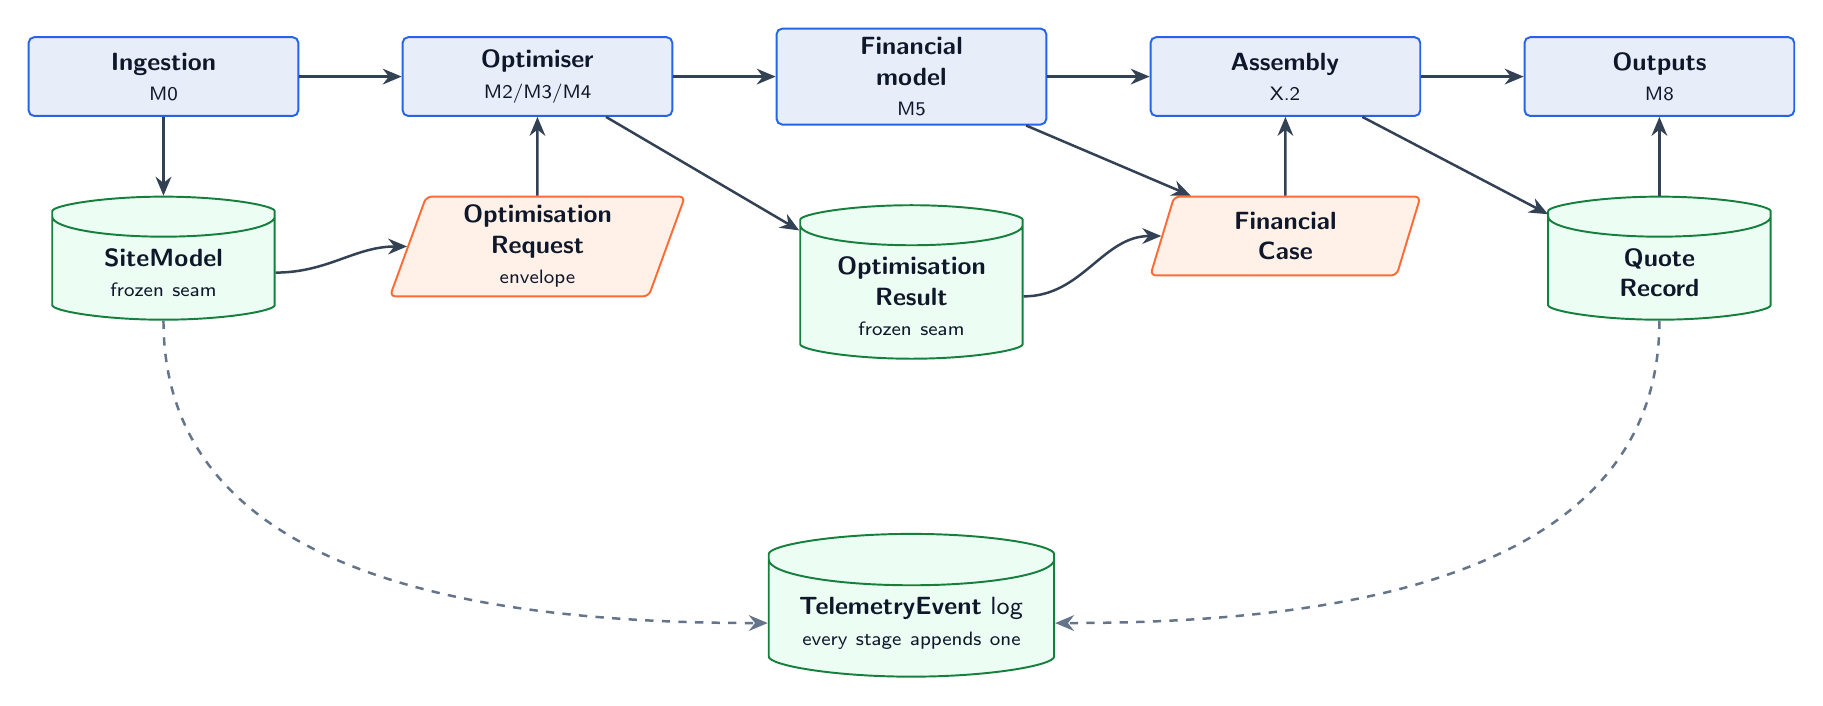
\begin{tikzpicture}[node distance=7mm and 13mm]
  % stages along the spine (processes)
  \node[proc] (ingest) {\textbf{Ingestion}\\\scriptsize M0};
  \node[proc, right=of ingest] (engine) {\textbf{Optimiser}\\\scriptsize M2/M3/M4};
  \node[proc, right=of engine] (finance) {\textbf{Financial}\\\textbf{model}\\\scriptsize M5};
  \node[proc, right=of finance] (assembly) {\textbf{Assembly}\\\scriptsize X.2};
  \node[proc, right=of assembly] (outputs) {\textbf{Outputs}\\\scriptsize M8};

  % the contracts flowing between them (data, on the spine)
  \node[store, below=10mm of ingest, draw=nodeStoreBd, fill=nodeStore, text width=26mm, minimum width=28mm] (site)
     {\textbf{SiteModel}\\\scriptsize frozen seam};
  \node[io, below=10mm of engine, text width=26mm, minimum width=28mm] (req)
     {\textbf{Optimisation}\\\textbf{Request}\\\scriptsize envelope};
  \node[store, below=10mm of finance, draw=nodeStoreBd, fill=nodeStore, text width=26mm, minimum width=28mm] (res)
     {\textbf{Optimisation}\\\textbf{Result}\\\scriptsize frozen seam};
  \node[io, below=10mm of assembly, text width=26mm, minimum width=28mm] (fin)
     {\textbf{Financial}\\\textbf{Case}};
  \node[store, below=10mm of outputs, text width=26mm, minimum width=28mm] (quote)
     {\textbf{Quote}\\\textbf{Record}};

  % spine flow between stages
  \draw[flow] (ingest) -- (engine);
  \draw[flow] (engine) -- (finance);
  \draw[flow] (finance) -- (assembly);
  \draw[flow] (assembly) -- (outputs);

  % stage produces / consumes contract (vertical seams)
  \draw[flow] (ingest) -- (site);
  \draw[flow] (site.east) to[out=0,in=180] (req.west);
  \draw[flow] (req) -- (engine);
  \draw[flow] (engine) -- (res);
  \draw[flow] (res.east) to[out=0,in=180] (fin.west);
  \draw[flow] (finance) -- (fin);
  \draw[flow] (fin) -- (assembly);
  \draw[flow] (assembly) -- (quote);
  \draw[flow] (quote) -- (outputs);

  % telemetry record, fed by all stages
  \node[store, below=22mm of res, fill=nodeStore, draw=nodeStoreBd, text width=34mm, minimum width=36mm] (tel)
     {\textbf{TelemetryEvent} log\\\scriptsize every stage appends one};
  \draw[flowback] (site.south) to[out=-90,in=180] (tel.west);
  \draw[flowback] (quote.south) to[out=-90,in=0] (tel.east);
\end{tikzpicture}}
\caption{The data-contract backbone. Each stage along the top produces a record (below it) that the next stage consumes; the two cylinders marked ``frozen seam'' (SiteModel and OptimisationResult) are the shared contracts between the two halves of the team. Every stage also appends to the append-only TelemetryEvent log.}
\label{fig:backbone}
\end{figure}

\subsection{OptimisationRequest and OptimisationResult}

The \textbf{OptimisationRequest} is the envelope handed to the engine: an embedded, already-validated SiteModel, the assumption version to price against, the list of value streams requested, an optional scenario reference, and a solve mode (baseline mock, or the real production engine). It carries nothing the engine does not need; the sizing search space and the objective live inside the engine, not in the envelope.

The \textbf{OptimisationResult} is what the engine returns and the second frozen seam. It carries the chosen battery as three flat numbers (power in kW, energy in kWh, duration in hours), a reference to the full half-hourly dispatch (the heavy schedule itself is dropped at the seam, only its content hash survives), the per-stream value results, the binding constraints, the gated-upside register, and the solver outcome and run metadata. It carries an \textbf{implementation level} (baseline / in progress / production) and a \textbf{bankable status}. Two rules are enforced: a baseline-level result can never be marked a bankable candidate, and the gated-upside register may only contain the three genuinely gated streams.

\begin{keyidea}[Firmness, gated upside, and the priced floor]
Each value stream carries a \emph{firmness}: firm, contracted, conditional, or excluded. The financial model's ``priced floor'' counts only firm and contracted income; conditional and gated streams are upside held out of the floor. Three streams -- wholesale/P415, the balancing mechanism, and ancillary services -- are \emph{gated upside}: they need a route-to-market partner that does not yet exist, so they live in a separate register and the contract forbids them ever being marked firm. This is how the platform keeps speculative income out of a bankable number by construction.
\end{keyidea}

\subsection{The dispatch power convention and the value accounting}

Two conventions in the result deserve to be stated plainly, because later chapters rely on them.

First, the \textbf{dispatch power convention}. When the optimiser's representative dispatch day is persisted for charting, each half-hour records the battery's power as \textbf{two separate non-negative series}: \code{charge\_kw}, the power the battery is drawing in, and \code{discharge\_kw}, the power it is pushing out to serve load or export. A reader of any dispatch series tells at a glance whether the battery is storing or earning by which series carries the power -- and because both fields are plain magnitudes, the contract's no-negatives rule applies to them unchanged, with no signed exception to remember. (A signed single series, positive for discharge, is a derived view a chart may compute; it is not what the contract stores.)

Second, the \textbf{value accounting}. The result reports value broken out per income stream, and the rule is that the per-stream figures must reconcile: the sum of value across the streams must equal the reported total value. There is no slack line and no rounding bucket. If a stream contributes income, it appears as a stream; the total is never larger than the parts add up to. This is what lets the underwriting pack show ``income by source'' and the customer proposal show ``total saving'' from the same record and have them agree.

\subsection{FinancialCase, QuoteRecord and TelemetryEvent}

The \textbf{FinancialCase} is the underwriting output built around a result. It insists on distributions, not point estimates: both a P50 (central) and a P90 (cautious) annual cashflow series are mandatory and must be the same length, and the debt cover ratio (DSCR, the multiple by which cash covers loan repayments, measured on the cautious P90 case) is a first-class summary. Cashflows may be negative -- year zero is the capital outlay -- which is the second documented exception to the no-negatives rule. It also carries the recommended price and structure, the debt assumptions, and the covenant check.

The \textbf{QuoteRecord} binds one run together: the site id, the embedded result and financial case, the data tier, the determinism hashes (a hash of the inputs, the assumption version, the code version), and an append-only history of lifecycle states. A handful of optional projections ride along for the web charts -- the full evaluated sizing grid and a representative dispatch day -- added without changing the quote's identity because they are excluded from the hash. One rule fires: an underwritten quote built from a coarse T0 site must carry an explicit warning, because T0 data is too thin to underwrite firmly.

The \textbf{TelemetryEvent} is one entry in the append-only log every stage writes to: the data tier at intake, the human minutes spent, the installer iterations, the outcome (won/lost with a reason), and the realised-versus-underwritten percentage once measurement supplies it. Time-to-quote is derived from the gap between events. This is the dataset that lets the platform prove it is faster than manual quoting rather than assert it (Chapter~\ref{ch:telemetry}).

\begin{rebuild}[How to rebuild the contract layer]
\begin{enumerate}
  \item \textbf{Define one base model} that forbids unknown fields and carries a single shared \code{schema\_version} string. Every contract inherits it. This single decision delivers the ``strict by construction'' guarantee.
  \item \textbf{Close every vocabulary as an enumeration} -- data tiers, market streams, firmness, consent states, lifecycle states, and so on -- so an unknown value is a validation error, never a pass-through.
  \item \textbf{Build the SiteModel as a composite:} identity fields, then the six required sub-records (load, tariff, connection, consents, physical gates, counterparty), then the optional bundles defaulting to all-unknown so additive fields never break old sites. Add \emph{no} archetype field.
  \item \textbf{Apply per-field rules:} non-negative on energy/power/money, with exactly two documented exceptions (connection headroom, and cashflows in the FinancialCase). Reject negative tariff rates and levies.
  \item \textbf{Apply record-level validators:} T2 requires half-hourly coverage metadata; T0 requires an annual total; an underwritten T0 quote requires a warning; a baseline result cannot be bankable; gated-upside may hold only the three gated streams.
  \item \textbf{Define the seam contracts} -- OptimisationRequest in, OptimisationResult out -- and treat SiteModel and OptimisationResult as frozen: a change bumps the shared version and re-runs a conformance test across both halves of the team.
  \item \textbf{Enforce the two conventions in tests:} dispatch power (two non-negative series, \code{charge\_kw} / \code{discharge\_kw}, never a signed single series) and value accounting (per-stream values sum exactly to the total).
  \item \textbf{Test:} round-trip every contract to JSON and back unchanged; assert each validator rejects its bad case and accepts its good case; assert an unknown field always raises; assert the example T0 and T2 sites validate.
\end{enumerate}
\end{rebuild}

\begin{plainnote}[Where the numbers are not]
Notice what this layer does \emph{not} contain: no prices, no rates, no thresholds, no formulas. The schema layer is pure shape. Every actual number lives in the versioned assumption library (Chapter~\ref{ch:assumptions}); every calculation lives in the engine and the financial model. A contract describes the box a number goes in, never the number. That separation is what makes the determinism and traceability guarantees possible.
\end{plainnote}

\chapter{Ingestion and data grading}
\label{ch:ingestion}
\modtag{M0}{Ingestion and data grading}{Agentic perimeter}

Every quote starts with whatever the customer and their installer can actually hand over. Sometimes that is a clean year of half-hourly meter readings; more often it is an annual energy total, a postcode, and a tariff sheet. This module is the front door. Its job is to take those raw inputs and turn them into one validated, honestly graded description of the site that the rest of the platform can compute on without ever second-guessing the data again.

The single rule that governs everything here is simple to state and absolute in practice: \textbf{ingestion never invents a number}. If a reading is missing, it is counted and reported, not filled in. If a whole input is absent, it becomes a written request for that data, not a guess. A site with thin data still gets a quote, but the quote is marked for what it is, and the platform tells the customer exactly which data would most improve it. This is what the manual calls \emph{honest degradation}: the platform always answers, and never pretends to know more than the data supports.

\begin{plainnote}
Think of ingestion as a careful clerk receiving a parcel. The clerk checks the contents against a packing list, notes anything damaged or missing on a slip, grades how complete the delivery is, and writes a short ``please also send'' note. The clerk never quietly slips a substitute item into the box to make the list look complete.
\end{plainnote}

\pipelinepos{Receives raw files from the customer/installer (a site description, optionally a real meter trace, optionally a price forecast). Hands a validated, graded \texttt{SiteModel} (Chapter~\ref{ch:contracts}) to the deterministic core.}

\begin{contract}
\textbf{In.} Up to three things, in any combination:
\begin{itemize}
  \item a \textbf{SiteModel JSON} file -- the structured description of the site (connection capacities, tariff, consents, counterparty);
  \item a \textbf{half-hourly meter CSV} -- the site's own real metered electricity, one row per 30-minute interval;
  \item an optional \textbf{wholesale price forecast} (CSV or JSON, e.g. a Modo export) -- used only as gated upside, never the priced floor (Chapters~\ref{ch:scenarios} and~\ref{ch:dispatch}).
\end{itemize}
\textbf{Out.} One validated \texttt{SiteModel} carrying: a graded data tier (T0, T1 or T2); measured load coverage folded into its \texttt{load\_data} block; a ranked list of the missing data that would most improve the quote; and a separate, structured validation report of every issue found. A confidential-data access log entry is written as a side effect of every meter read. Nothing that enters as missing leaves as a fabricated value.
\end{contract}

\section{Why a core artifact is born on the perimeter}

The \texttt{SiteModel} is the central artifact of the whole platform: everything downstream reads it, and it must be trustworthy. Yet ingestion lives on the \emph{agentic perimeter}, the AI-assisted, human-confirmed outer zone, not in the deterministic core. That looks like a contradiction, so it is worth resolving up front.

The reason is that the work ingestion does is exactly the messy, judgement-laden work the core is forbidden to touch. Real installer files arrive in inconsistent shapes, with odd column names, mislabelled units, gaps, and the occasional implausible reading. Cleaning that up, deciding that a column called \code{demand\_kw} means import power, asking the installer for the consent state, is perimeter work: assisted, schema-checked, and confirmed by a person.

The wall between the two zones is preserved by a strict division of labour. The perimeter is allowed to \emph{shape} data into the validated schema, but it is structurally unable to \emph{author a value}. A missing reading never becomes a plausible-looking guess; it becomes a typed warning or a ranked ask. By the time the \texttt{SiteModel} crosses into the core it is a pure, validated object with no fabricated content, so the determinism guarantee of the core is never compromised by the judgement that produced its input.

\begin{keyidea}
Ingestion produces a core artifact but does perimeter work. The contradiction dissolves once you see the boundary is not ``which artifact'' but ``which action'': shaping messy input into a strict schema is allowed; inventing a number to fill a gap is not. The output crossing into the core therefore contains only validated, measured, or explicitly-requested data, never a guess.
\end{keyidea}

\section{Loading a SiteModel JSON}

The structured path is the simplest. A single JSON object describing the site is read and validated against the versioned \texttt{SiteModel} schema (Chapter~\ref{ch:contracts}). Validation happens in two gates, and both must pass before the object is trusted.

\textbf{Gate one is the schema.} The schema is strict: it rejects unknown fields outright (a typo in a field name is an error, not a silent no-op), checks every type, and enforces the structural tier and coverage invariants (for instance, a site graded T2 must carry half-hourly coverage metadata; a T0 site must state an annual consumption figure). A failure here is reported with the exact field path and reason, never a generic ``invalid file''.

\textbf{Gate two is coherence.} A file can be schema-valid yet internally contradictory, and the schema alone cannot catch that. A second pass runs cross-field checks and records each finding as a typed issue with a stable code, a severity, and the field it concerns. The checks, and their severities, are listed in Table~\ref{tab:coherence}. An issue of severity \emph{error} causes the load to be rejected, distinctly from a schema failure, so the caller can tell ``wrong shape'' from ``shape fine, contents incoherent''. Warnings and informational findings never stop the load: they travel with the result so the pipeline can run and \emph{say} what is doubtful.

\begin{table}[H]
\centering
\caption{The cross-field coherence checks, run after the schema passes. Errors reject the load; warnings and info travel with the result.}
\label{tab:coherence}
\small\sffamily
\begin{tabularx}{\textwidth}{@{}L l L@{}}
\toprule
\textbf{Check} & \textbf{Severity} & \textbf{Why it matters} \\
\midrule
Exports but a generation consent reads ``not required'' & error & Physically incoherent: a site that exports must hold export consent. \\
Exports but no export MPAN recorded & warning & Export-side income cannot be firmed without the export meter point. \\
Import capacity (MIC) reads zero & warning & A connection that cannot import is implausible; confirm the figure. \\
Negative import headroom & info & Site is over-subscribed against its import limit at peak; noted, not blocked. \\
Graded T2 but no reference to the validated series & warning & The canonical meter trace should be pointed to before the quote is treated as firm. \\
Graded T0 yet carries half-hourly coverage & info & It may deserve a higher tier; re-grade from the meter summary. \\
Counterparty company number missing or malformed & warning & The credit mapping (Chapter~\ref{ch:finance}) keys off the registered entity. \\
Counterparty credit not yet assessed & warning & No credit band means no debt rate or tenor can be set; none is assumed. \\
\bottomrule
\end{tabularx}
\end{table}

A well-formed UK company number is checked only for shape (eight alphanumeric characters): a deterministic format sanity check, with no external lookup. Ingestion confirms the input looks right; it does not reach out to a registry and invent a fact.

\section{Folding in a real half-hourly meter trace}

The half-hourly (HH) trace is the most valuable input the platform takes: the site's own metered electricity, one row every 30 minutes. A full validated year of it is what separates a banded, indicative quote from a firm, underwritten one. Ingestion treats it as a first-class input with its own load, validate, summarise, fold sequence.

\subsection{Load: normalise without altering}

The CSV is read and its columns are matched case-insensitively against a set of known aliases, so a column headed \code{demand\_kw}, \code{kw\_import} or \code{settlement\_datetime} is recognised and renamed to the canonical name. Exactly one thing is required besides a timestamp: either import power (\code{import\_kw}) or import energy per interval (\code{import\_kwh}). Export, a site-load column, a meter id and a quality flag are optional. Three rules hold without exception during the load:

\begin{itemize}
  \item \textbf{Timestamps must parse, for every row.} A file with unparseable timestamps is rejected with an error naming the first offending values. Timestamps are never coerced and then guessed.
  \item \textbf{The row count is preserved exactly.} No row is added, dropped or re-timed. Blank or non-numeric load cells become null and are counted later; they are not filled.
  \item \textbf{Energy-to-power is a labelled transform, not a fabricated value.} When only energy per interval is given, average power is derived deterministically as energy times $60$ divided by the interval length in minutes (which is simply $\times 2$ for 30-minute periods), and the series is labelled as derived from energy rather than measured as power.
\end{itemize}

\begin{caution}[Timestamps, timezones and daylight saving]
Naive timestamps (no UTC offset) are taken as the site's local clock, labelling the start of each half hour, and are never re-timed. A uniform UTC offset is kept as a timezone-aware series, and a file that mixes offsets (the +00:00/+01:00 pattern of a UK export spanning a clock change) is converted to a single UTC axis without dropping a row; unparseable values still reject the file. Daylight saving follows from this: a timezone-aware trace is physically continuous across a clock change, so the dispatch engine (Chapter~\ref{ch:dispatch}) sees no false gap there, while a naive local trace jumps by one hour at the spring transition, which the engine treats as one conservative segment boundary rather than inventing the missing labels. Tariff banding always reads the GB local clock: timezone-aware timestamps are converted to Europe/London before banding.
\end{caution}

\subsection{Validate: count integrity, never repair it}

A coverage pass then measures the trace without touching it. Over the observed window (first timestamp to last) it works out how many intervals \emph{should} be present on the declared grid, compares that with how many distinct timestamps are actually present, and reports the difference as missing intervals. It also counts duplicate timestamps (surplus rows sharing a timestamp), infers the real median spacing of the grid to detect a file that is not actually half-hourly, and computes the calendar span, an approximate month count, and a completeness percentage. The defining property: every one of these is a \emph{count}, never a correction. The formulae are gathered in Table~\ref{tab:coverage}.

\begin{table}[H]
\centering
\caption{Coverage metrics computed from a loaded half-hourly trace. Every figure is measured; none alters the data.}
\label{tab:coverage}
\small\sffamily
\begin{tabularx}{\textwidth}{@{}l L@{}}
\toprule
\textbf{Metric} & \textbf{How it is computed} \\
\midrule
Present intervals & Count of distinct, parseable timestamps. \\
Duplicate timestamps & Total rows minus present intervals. \\
Expected intervals & $\mathrm{round}(\text{window seconds} \div \text{step seconds}) + 1$, on the declared grid. \\
Missing intervals & $\max(\text{expected} - \text{present},\, 0)$; counted, never back-filled. \\
Completeness \% & $\min(\text{present} \div \text{expected} \times 100,\ 100)$. \\
Inferred grid (minutes) & Median gap between consecutive distinct timestamps; flags a non-HH file. \\
Coverage days / months & Window length in days; months $\approx$ days $\div\ 30.44$. \\
\bottomrule
\end{tabularx}
\end{table}

\subsection{Summarise: load statistics plus a report}

A summary step layers the load statistics on top of the coverage (maximum, minimum and mean import power; maximum export; counts of null and of negative readings) and assembles the validation report. Each integrity concern becomes a typed warning: duplicate timestamps, missing intervals, null readings, negative import or export (negative import is physically unusual for a consuming site, so it is flagged unless the caller explicitly allows it), and an inferred grid that does not match the expected one. Crucially these are \emph{warnings, not failures}: a flawed trace is described in full and the run continues.

\subsection{Fold and re-grade}

Finally the measured coverage is folded into the \texttt{SiteModel}'s load block and the tier is re-graded from the real data. The fold preserves any prior figure the meter summary does not itself carry (a stated annual consumption, a known peak import or export), and it re-validates the whole site through the schema rather than patching fields in place, so an inconsistent fold (for example, a trace so sparse it grades back to T0 with no annual figure anywhere) raises a validation error rather than minting a silently invalid site. The annual energy figure is deliberately left unset by the fold unless it genuinely came from the series or a stated number: it is never inferred from a partial trace.

\section{Grading the data tier}

The tier is the platform's honest, one-word verdict on how much the data can support. It is graded by a pure function of the meter summary, so the same data always yields the same tier. The boundaries are exact and worth stating precisely, because they decide whether a quote can be underwritten.

\begin{table}[H]
\centering
\caption{The three data tiers and the exact rule that assigns each. T1 and T2 are distinguished by the validated-twelve-month bar.}
\label{tab:tiers-ingestion}
\small\sffamily
\begin{tabularx}{\textwidth}{@{}l L L@{}}
\toprule
\textbf{Tier} & \textbf{Plain meaning} & \textbf{Exact rule} \\
\midrule
\textbf{T0} & Coarse: annual energy, tariff, postcode; no usable meter trace. & No summary at all, or fewer than two present intervals (a single stray reading is not a series). \\
\textbf{T1} & Partial: genuine half-hourly data, but below the validated-twelve-month bar. & At least two present intervals, but the full T2 test below is not met. \\
\textbf{T2} & Full: at least twelve validated months of half-hourly data passing the checks. & \emph{All three} of: present intervals $\ge 17\,520 - 96$ (twelve months of 48 half-hours, less a $\pm 2$-day tolerance); calendar span $\ge 363$ days; completeness $\ge 90\%$. \\
\bottomrule
\end{tabularx}
\end{table}

Three details earn their place. First, the period floor of \textbf{17\,520} is simply $48 \times 365$: the number of half-hours in a year. The small tolerance of $\pm 96$ periods (about two days) lets a genuine year that is a handful of intervals short, through daylight-saving or a leap year, still grade T2. Second, the \emph{calendar-span} gate is separate from the interval count on purpose: a dense file recorded every few minutes over a short window could otherwise rack up 17\,520 intervals without spanning a year, and the span gate of at least 363 days rejects that. Third, the function never \emph{upgrades} a tier on the strength of data it does not have: in particular, the absence of a real trace lands at T0 regardless of any stated annual figure.

\begin{caution}[Tier boundaries are structure, not assumptions]
The tier numbers (48 half-hours a day, 17\,520 a year, the 90\% completeness floor) are \emph{structural calendar boundaries}, not pricing assumptions, and they carry no money. They therefore live, labelled, in the ingestion code rather than in the versioned assumption library (Chapter~\ref{ch:assumptions}), the same precedent the platform uses for other labelled structural constants. Whether the completeness floor should be versioned alongside the priced assumptions is an open question for the team; until resolved it is a documented default.
\end{caution}

\begin{figure}[H]
\centering
\resizebox{\textwidth}{!}{%
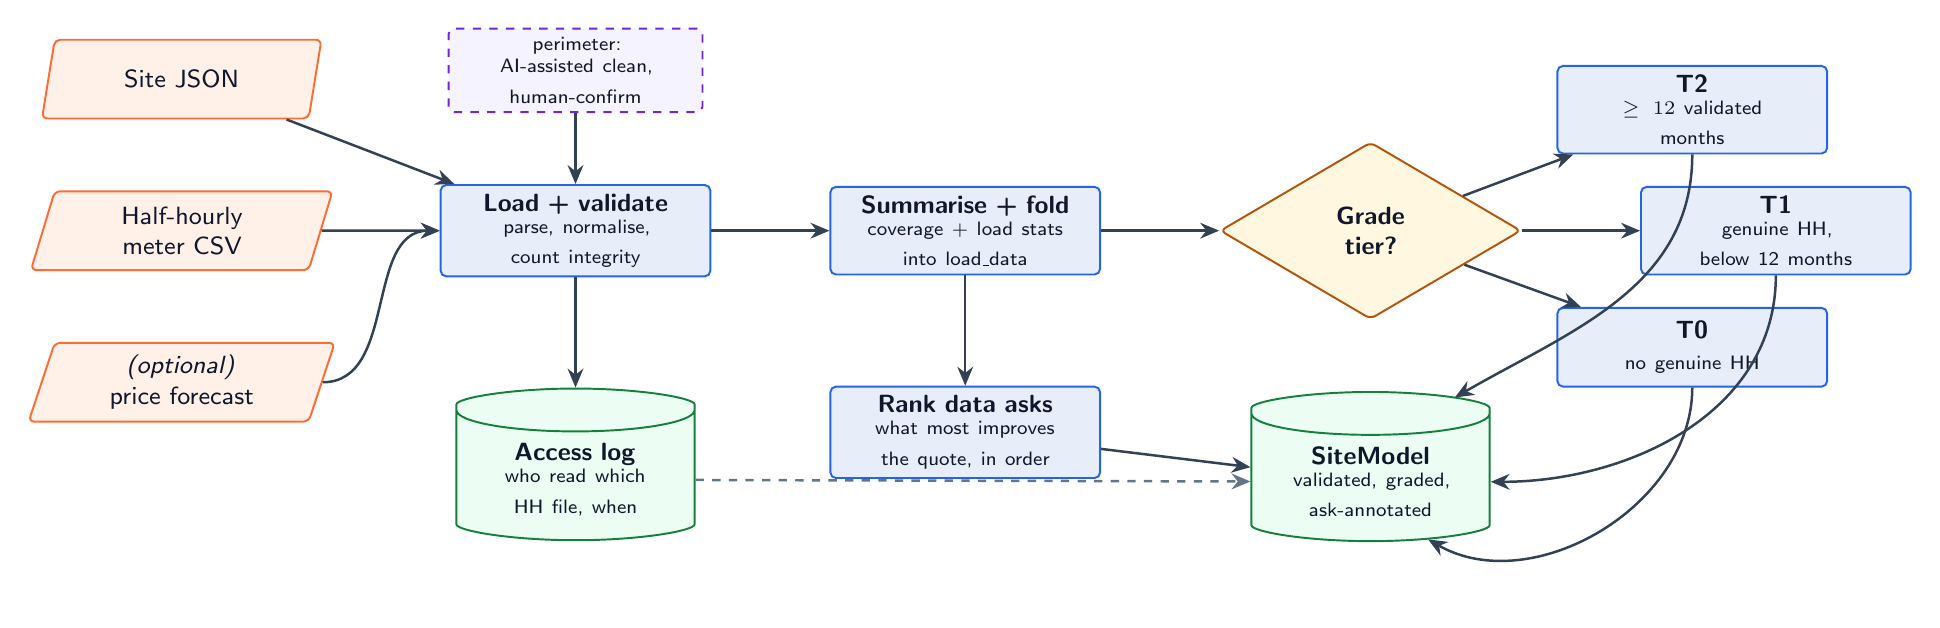
\begin{tikzpicture}[node distance=9mm and 15mm]
  % inputs
  \node[io] (sitejson) {Site JSON};
  \node[io, below=of sitejson] (hhcsv) {Half-hourly\\meter CSV};
  \node[io, below=of hhcsv] (fcast) {\textit{(optional)}\\price forecast};

  % validate stage
  \node[proc, right=of hhcsv] (validate) {\textbf{Load + validate}\\\scriptsize parse, normalise,\\\scriptsize count integrity};
  \node[ext, above=of validate] (clean) {\scriptsize perimeter:\\AI-assisted clean,\\human-confirm};

  % fold + summarise
  \node[proc, right=of validate] (fold) {\textbf{Summarise + fold}\\\scriptsize coverage + load stats\\\scriptsize into load\_data};

  % grade gate
  \node[decide, right=of fold] (grade) {\textbf{Grade}\\\textbf{tier?}};

  % tier outcomes
  \node[proc, above right=4mm and 14mm of grade] (t2) {\textbf{T2}\\\scriptsize $\ge 12$ validated\\\scriptsize months};
  \node[proc, right=of grade] (t1) {\textbf{T1}\\\scriptsize genuine HH,\\\scriptsize below 12 months};
  \node[proc, below right=4mm and 14mm of grade] (t0) {\textbf{T0}\\\scriptsize no genuine HH};

  % rank asks + sitemodel
  \node[proc, below=14mm of fold] (rank) {\textbf{Rank data asks}\\\scriptsize what most improves\\\scriptsize the quote, in order};
  \node[store, below=of grade] (sitemodel) {\textbf{SiteModel}\\\scriptsize validated, graded,\\\scriptsize ask-annotated};
  \node[store, below=14mm of validate] (alog) {\textbf{Access log}\\\scriptsize who read which\\\scriptsize HH file, when};

  % main flow
  \draw[flow] (sitejson) -- (validate);
  \draw[flow] (hhcsv) -- (validate);
  \draw[flow] (fcast) to[out=0,in=180] (validate);
  \draw[flow] (clean) -- (validate);
  \draw[flow] (validate) -- (fold);
  \draw[flow] (fold) -- (grade);
  \draw[flow] (grade) -- (t2);
  \draw[flow] (grade) -- (t1);
  \draw[flow] (grade) -- (t0);
  \draw[flow] (t1) to[out=-90,in=0] (sitemodel.east);
  \draw[flow] (t2) to[out=-90,in=30] (sitemodel.north east);
  \draw[flow] (t0) to[out=-90,in=-30] (sitemodel.south east);
  \draw[flow] (fold) -- (rank);
  \draw[flow] (rank) -- (sitemodel);
  \draw[flow] (validate) -- (alog);
  \draw[flowback] (alog) -- (sitemodel);
\end{tikzpicture}}
\caption{The ingestion flow. Raw inputs are loaded and validated (with optional AI-assisted cleaning on the perimeter), summarised and folded, then the tier is graded at a decision gate. The ranked data asks and a confidential-data access entry travel into the final, graded \texttt{SiteModel}.}
\label{fig:ingestion-flow}
\end{figure}

\section{The ranked missing-data asks}

Whatever the tier, ingestion inspects the assembled site and produces a \textbf{ranked data ask}: the prioritised list of the inputs that, if supplied, would most improve the quote. This turns a vague installer back-and-forth into a precise, ordered request. Each ask records what is missing, \emph{why it matters}, and \emph{what it blocks} downstream. The ranking is deterministic, ordered by a fixed impact priority and a stable tie-breaker, so the same site always yields the same ask order. The catalogue, in priority order, is in Table~\ref{tab:asks}.

\begin{table}[H]
\centering
\caption{The ranked data-ask catalogue, highest impact first. The wholesale forecast ask appears only when wholesale analysis has been requested.}
\label{tab:asks}
\small\sffamily
\begin{tabularx}{\textwidth}{@{}c L L@{}}
\toprule
\textbf{Rank} & \textbf{Ask} & \textbf{What it unlocks / blocks} \\
\midrule
1 & Twelve months of half-hourly meter data & Tier T2 and an underwritten (rather than indicative) quote. \\
2 & Full tariff: standing charge, unit rates, DUoS bands, levy lines & The import-side bankable floor cannot be priced without it. \\
3 & Connection capacities: MIC, MEC, ASC & Bounds the dispatch and prices headroom value where it binds. \\
4 & DNO region & The DUoS band structure and whether a local-flexibility tender is open. \\
5 & Export status: G99/G100 consent and export MPAN & Gates export-side and wholesale upside streams. \\
6 & Supplier consent & A listed condition before an underwritten quote becomes firm. \\
7 & Physical gates: footprint, fire separation, access & Listed pass/fail conditions on an underwritten quote. \\
8 & Counterparty legal entity and company number & The deterministic credit-to-rate/tenor mapping (Chapter~\ref{ch:finance}). \\
9 & Wholesale price forecast file & Only if wholesale analysis is requested; gated upside, never the floor. \\
\bottomrule
\end{tabularx}
\end{table}

The ordering encodes the platform's priorities: the data tier first (the single biggest fidelity lever), then the priced floor (tariff and connection), then the gates and consents, then counterparty credit, and finally the gated upside last of all. The counterparty asks are mutually exclusive by design: a site with no registered identity yields the identity ask alone, not both the identity ask and a separate credit-band ask, so the request stays clean. The same ranked list is rendered two ways: a short ordered set of strings written onto the \texttt{SiteModel} itself, and a fuller human-readable block (each ask with its reason, detail and blocked items) suitable for an installer email or the customer memo.

\begin{caution}[The forecast is upside, never the floor]
The wholesale price forecast is the only input whose ask is conditional, and it is ranked last for a reason. Wholesale and balancing income is treated as \emph{gated upside}: priced from a forecast the customer supplies, never generated, and never part of the bankable floor (Chapters~\ref{ch:scenarios} and~\ref{ch:dispatch}). A forecast that is loaded is pinned with a content hash and its source and version recorded, so a quote can cite exactly which curve it used; missing prices stay missing and are warned, and interpolation happens only when explicitly asked for, is labelled on every filled point, and never extrapolates beyond the known range.
\end{caution}

\section{The confidential-data access log}

A site's half-hourly trace is confidential commercial data, so the platform treats every read of it as an auditable event. Each successful meter-file load writes an append-only entry recording the file, the action, the site and the actor responsible, the row count, whether the data is personal, and a wall-clock timestamp. The log is written \emph{by construction} as a side effect of loading, so it cannot be bypassed by a caller who forgets to record it.

Two properties keep this clean. First, the log is \textbf{metadata about access, never an input to pricing}: it carries a wall-clock time and is deliberately kept out of every quote and run hash, so it can never perturb a deterministic result. Second, it is \textbf{fail-closed} when persistence is configured: if an audit destination is set but cannot be written, the read does not silently proceed unaudited. By default the sink is in-memory only, so library and test use have no side effects; pointing an environment variable at a file additionally appends each entry as one JSON line, following the platform's files-first convention.

\section{Honest degradation in practice}

The honest-degradation principle is not a slogan here; it is the observable behaviour of the module. A bad half-hourly file is the clearest illustration. Suppose an installer sends a meter CSV with a block of unparseable timestamps. The load rejects \emph{that file} with a precise error naming the offenders, the fold is simply not performed, and the run continues from the structured site description alone, landing at whatever tier the remaining data supports (often T0) with the twelve-months-of-half-hourly ask ranked first. The customer still gets a quote, it is marked for what it is, and the top of the data ask tells them exactly what to send to improve it. A merely flawed (but readable) trace behaves even more gently: its duplicates, gaps and odd readings become warnings that travel with the result, and the trace is still used. The platform reports the problem, skips only what it genuinely cannot use, and never stops.

\begin{rebuild}
To re-implement this module from scratch:
\begin{enumerate}
  \item \textbf{Define the typed vocabulary first.} An exception hierarchy with a distinct subclass per input kind (site / meter / forecast), and a validation report holding severity-tagged issues, each with a stable machine-readable code, a message, and the field it concerns. The report is advisory: it never raises by itself.
  \item \textbf{Build the SiteModel loader as two gates.} Gate one: strict schema validation (reject unknown fields; enforce tier/coverage invariants); report failures with the exact field path. Gate two: cross-field coherence checks (Table~\ref{tab:coherence}); an error-severity finding rejects the load, distinct from a schema failure; warnings and info travel on.
  \item \textbf{Build the half-hourly path as load, validate, summarise, fold.} On load: canonicalise columns by case-insensitive alias; require a timestamp plus one of import power or import energy; parse every timestamp strictly (raise, naming offenders, on failure); preserve the row count exactly; derive power from energy as a labelled transform ($\times\,60/\text{interval minutes}$). On validate: compute the coverage metrics of Table~\ref{tab:coverage} as counts, never corrections. On summarise: add load statistics and emit a warning per integrity concern (duplicates, gaps, nulls, negatives, irregular grid). On fold: rebuild the load block from measured coverage, preserve prior annual/peak figures the summary lacks, and re-validate the whole site through the schema rather than patching fields.
  \item \textbf{Grade the tier as a pure function of the summary} using the exact rule in Table~\ref{tab:tiers-ingestion}: under two intervals (or no summary) is T0; T2 requires the period floor ($\ge 17\,520 - 96$) \emph{and} a span of $\ge 363$ days \emph{and} completeness $\ge 90\%$, all three; everything else genuine is T1. Never upgrade on data you do not have.
  \item \textbf{Detect missing data, then rank it.} Inspect the assembled site for each category in Table~\ref{tab:asks}; emit a typed missing item carrying why-it-matters and what-it-blocks; sort by a fixed impact priority then a stable id tie-breaker; assign contiguous ranks. Keep the counterparty identity and credit-band asks mutually exclusive. List the wholesale forecast only when wholesale analysis is requested. Write the ranked list onto the SiteModel and offer a human-readable rendering.
  \item \textbf{Log every confidential meter read by construction} as an append-only entry (file, actor, site, rows, timestamp), written inside the loader so it cannot be skipped; keep it out of every hash; fail-closed when a persistent sink is configured.
\end{enumerate}
\textbf{What to test.} Identical input gives an identical tier and an identical ask order (determinism). A loaded frame has exactly the input row count. Missing intervals are counted, never filled. An unparseable timestamp raises and names offenders. The T1/T2 boundary flips precisely at the period, span and completeness thresholds. An incoherent-but-schema-valid site is rejected distinctly from a schema-invalid one. A bad meter file is reported and skipped while the run completes. A meter read always leaves an access-log entry, and that entry never changes a quote hash.
\end{rebuild}

This validated, graded, ask-annotated \texttt{SiteModel} is the object the rest of the platform computes on. Its precise shape, and the invariants the schema enforces, are the subject of Chapter~\ref{ch:contracts}; the assumption versions that turn it into priced numbers follow in Chapter~\ref{ch:assumptions}.

\chapter{The assumption library}
\label{ch:assumptions}
\modtag{X.1}{Assumption library}{Cross-cutting}

Every quote the platform produces is built from numbers: how much a battery costs to install, how quickly it degrades, what a unit of avoided peak charge is worth, the interest rate a lender charges a given customer, the return the price must clear. There are dozens of such numbers, and almost every stage of the pipeline needs some of them. The obvious way to supply them is to write each value where it is used. The platform forbids that absolutely. Instead every number lives in one place: a single, versioned \emph{assumption library}.

The rule is short and has no exceptions. \textbf{No pricing, finance, dispatch, sizing or output module may hold a number of its own.} If a stage needs the installed cost of a battery, it does not write \code{500000} into its code; it asks the library for \code{battery\_capex.installed\_cost} and uses whatever comes back. A value can therefore be found, reviewed, corrected and audited in exactly one location, and every quote can say which exact set of values it was built from.

\begin{plainnote}
Think of the library as the single master rate-card the whole business prices from. Nobody is allowed to keep a private copy of a rate scribbled in a drawer. When the card is reissued it gets a new edition number printed on it, and every quote staples on a note saying which edition it used. If the card later changes by more than a hair, quotes priced on the old edition are not quietly patched; they are re-quoted against the new one.
\end{plainnote}

\pipelinepos{Sits beside the whole deterministic core. Loaded once at the start of a run; read by ingestion's plausibility gates, the value stack, dispatch, sizing, the scenario engine, the financial model and credit. Its version tag is stamped onto the resulting quote record (Chapter~\ref{ch:provenance}).}

\begin{contract}
\textbf{In.} A version string naming a release, for example \code{gb\_v0\_1}. The loader resolves it to a single file on disk (\fpath{assumptions/<version>.yaml}; \code{.yml} and \code{.json} are also accepted).\\
\textbf{Out.} One validated, in-memory \emph{assumption library} object: a release header plus every section of numbers, each number wrapped in its full documentation (value, unit, source, review status, owner, confidence, review date, notes). The same object also answers the question ``does a quote priced on version A need repricing against version B?''. If the named version is missing, malformed, or omits any required section, loading fails loudly rather than returning a partial set.
\end{contract}

\section{Why one versioned source, and nothing else}

Two of the platform's five guarantees (Chapter~\ref{ch:overview}) depend directly on this module: \emph{traceability} -- every number can be tied back to what produced it -- and \emph{one versioned source for every assumption}. A private constant scattered in code breaks both at once. If a discount rate were written into the financial model and also, slightly differently, into a spreadsheet that generated a price curve, the two would drift apart, and no quote could honestly say which value it used. Worse, a lender auditing the pack could not reproduce a figure without reading the source code line by line.

Centralising every number removes that whole class of problem. Because the library is the only door to these values, three properties follow for free:

\begin{itemize}
  \item \textbf{Consistency.} Two stages that need the same number get the same number, by construction, because there is only one.
  \item \textbf{Auditability.} Every value carries its own provenance: where it came from, who owns confirming it, how confident the platform is in it, and when it was last looked at. No number is undocumented.
  \item \textbf{Reproducibility.} A quote records the library version it used. Anyone holding that version can recompute the quote and get the identical answer, because the inputs are fully pinned (Chapter~\ref{ch:provenance}).
\end{itemize}

\begin{keyidea}[No private constants, ever]
The single most important rule of this module is what it forbids elsewhere. If any module in the deterministic core ever contains a bare numeric literal that influences a priced figure, the abstraction has failed. Every such number must be fetched from the versioned library by section and name, so that changing it is a versioned event and every quote can name the version it trusted.
\end{keyidea}

\section{What one assumption looks like}

The library is not a flat list of numbers. Each value is a small, self-documenting record, and every one of its descriptive fields is \emph{required}: a number with a missing source or no review status is a loading error, not an accepted entry. This is how the platform enforces ``no number is undocumented''. The fields are listed in Table~\ref{tab:assumptionfields}.

\begin{table}[H]
\centering
\caption{The fields every assumption entry must carry. All are required; a missing field fails validation, so no number can enter the library undocumented.}
\label{tab:assumptionfields}
\small\sffamily
\begin{tabularx}{\textwidth}{@{}l L@{}}
\toprule
\textbf{Field} & \textbf{What it records} \\
\midrule
\code{value} & The number itself, or a small structured value (for example a rate-and-tenor pair per credit band, or a factor per battery duration). \\
\code{unit} & The unit the value is expressed in: \code{GBP/MW}, \code{ratio}, \code{percent}, \code{cycles/yr}, and so on. A redenomination is treated as a material change even at the same number. \\
\code{source} & Where the value came from: a named document, a data provider, or the honest word \code{placeholder}. \\
\code{status} & Its place on the review lifecycle: \emph{placeholder}, \emph{needs\_review}, or \emph{confirmed}. \\
\code{owner\_or\_reviewer} & Who is responsible for confirming it. \\
\code{confidence} & Low, medium or high confidence in the value as it stands. \\
\code{last\_reviewed} & The date the entry was last examined. \\
\code{notes} & Context, caveats, and what would raise the confidence. \\
\bottomrule
\end{tabularx}
\end{table}

\begin{plainnote}
The status field carries an honest health warning. A value marked \emph{placeholder} is a stand-in chosen so the pipeline can run end to end; it is usable but must never be dressed up as a confirmed, bankable number. Values move along the lifecycle \emph{placeholder} $\rightarrow$ \emph{needs\_review} $\rightarrow$ \emph{confirmed} as they are sourced and checked. The current GB release, \code{gb\_v0\_1}, is entirely placeholders, which is exactly why every quote it produces is deliberately marked \emph{not bankable}.
\end{plainnote}

\section{Loading and validating a release}

A release is a single file, named for its version, holding a release header plus a fixed set of named sections of assumptions. Loading it is a deliberately strict, single-door operation, so that a malformed or incomplete library is caught at the start of a run rather than producing a quietly wrong quote. The loader performs the steps in Figure~\ref{fig:assumload}.

\begin{figure}[H]
\centering
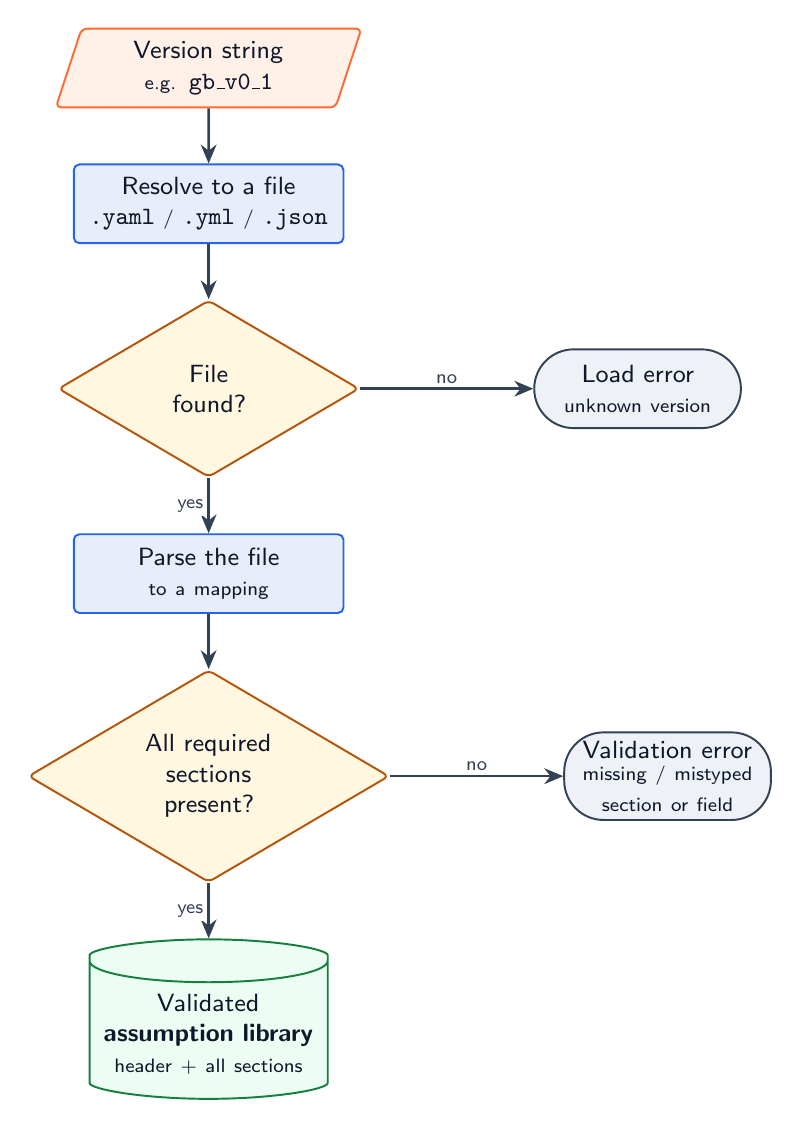
\begin{tikzpicture}[node distance=7mm and 14mm]
  \node[io] (ver) {Version string\\\scriptsize e.g. \code{gb\_v0\_1}};
  \node[proc, below=of ver] (resolve) {Resolve to a file\\\scriptsize \code{.yaml} / \code{.yml} / \code{.json}};
  \node[decide, below=of resolve] (exists) {File\\found?};
  \node[proc, below=of exists] (parse) {Parse the file\\\scriptsize to a mapping};
  \node[decide, below=of parse] (sections) {All required\\sections\\present?};
  \node[store, below=of sections] (lib) {Validated\\\textbf{assumption library}\\\scriptsize header + all sections};
  \node[term, right=22mm of exists] (fail1) {Load error\\\scriptsize unknown version};
  \node[term, right=22mm of sections] (fail2) {Validation error\\\scriptsize missing / mistyped\\section or field};

  \draw[flow] (ver) -- (resolve);
  \draw[flow] (resolve) -- (exists);
  \draw[flow] (exists) -- node[flowlabel,left]{yes} (parse);
  \draw[flow] (exists) -- node[flowlabel,above]{no} (fail1);
  \draw[flow] (parse) -- (sections);
  \draw[flow] (sections) -- node[flowlabel,left]{yes} (lib);
  \draw[flow] (sections) -- node[flowlabel,above]{no} (fail2);
\end{tikzpicture}
\caption{Loading a release is strict and fails loudly. A version that has no file, a file that will not parse, or a file missing any required section never yields a usable library; there is no partial load.}
\label{fig:assumload}
\end{figure}

The release header records the market (\code{GB}), the version string, the release date, and the currency. The sections that follow are not free-form: the library schema names every section that a valid GB release must carry, and each section is a labelled group of assumption entries. Because the sections are fixed and checked, a section that is missing, misspelt, or holding the wrong shape of data is a validation error. This is the mechanism behind ``all required sections must be present'': you cannot accidentally ship a release that forgot to state, say, the financing terms.

\begin{caution}[A new value means a new file, never an in-place edit]
A released library file is frozen. Correcting a value, confirming a placeholder, or adding an assumption is done by cutting a \emph{new versioned file} with a new version string, never by editing a file that has already produced quotes. This is what keeps old quotes honest: a quote pinned to \code{gb\_v0\_1} keeps reading exactly the numbers \code{gb\_v0\_1} held, no matter what later releases change. GB-specific values are \emph{content} in these files; the engine never branches on the market, so a new market is simply a new file, not new code.
\end{caution}

\section{The version tag travels onto every quote}

Loading happens once at the start of a run. The library is then read, but never altered, by every deterministic stage that needs a number. Figure~\ref{fig:assumfeed} shows the shape of that fan-out: one versioned store feeding the whole core, with its version string flowing through to the finished quote record.

\begin{figure}[H]
\centering
\resizebox{\textwidth}{!}{%
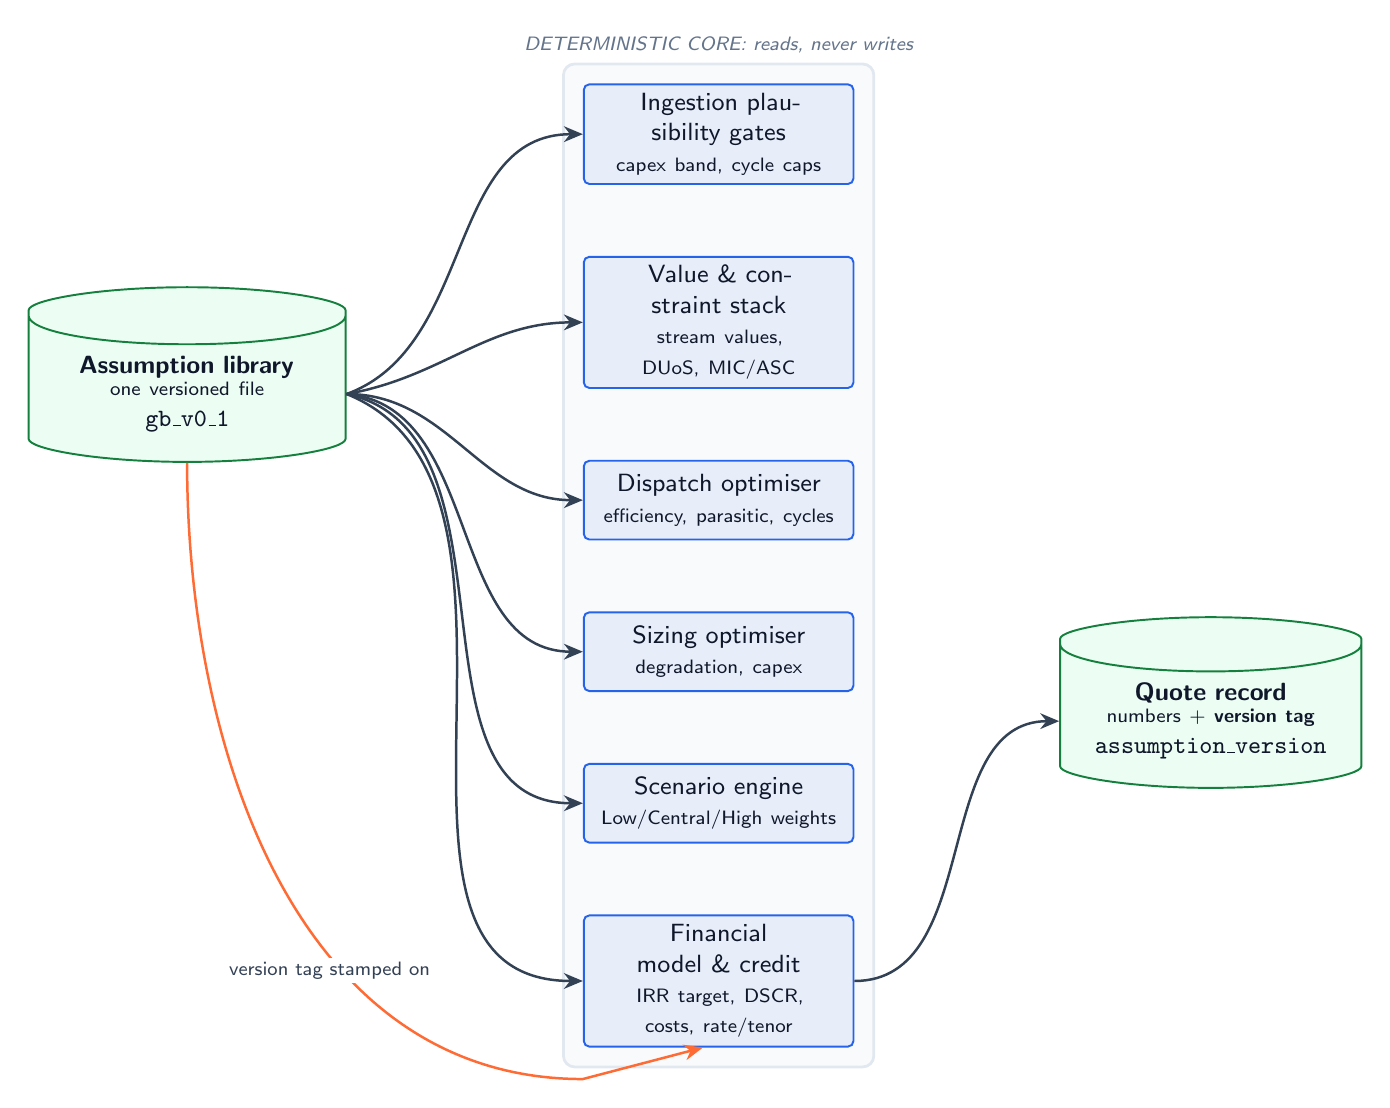
\begin{tikzpicture}[node distance=9mm and 16mm]
  % the store
  \node[store, fill=gridqGreenBg, draw=nodeStoreBd, minimum width=40mm, text width=38mm] (lib)
    {\textbf{Assumption library}\\\scriptsize one versioned file\\\scriptsize \code{gb\_v0\_1}};

  % consumer stages, stacked to the right
  \node[proc, right=30mm of lib, yshift=33mm] (gates) {Ingestion plausibility gates\\\scriptsize capex band, cycle caps};
  \node[proc, below=of gates] (value) {Value \& constraint stack\\\scriptsize stream values, DUoS, MIC/ASC};
  \node[proc, below=of value] (dispatch) {Dispatch optimiser\\\scriptsize efficiency, parasitic, cycles};
  \node[proc, below=of dispatch] (sizing) {Sizing optimiser\\\scriptsize degradation, capex};
  \node[proc, below=of sizing] (scen) {Scenario engine\\\scriptsize Low/Central/High weights};
  \node[proc, below=of scen] (fin) {Financial model \& credit\\\scriptsize IRR target, DSCR, costs, rate/tenor};

  % fan-out arrows
  \draw[flow] (lib.east) to[out=20,in=180] (gates.west);
  \draw[flow] (lib.east) to[out=10,in=180] (value.west);
  \draw[flow] (lib.east) to[out=0,in=180] (dispatch.west);
  \draw[flow] (lib.east) to[out=-5,in=180] (sizing.west);
  \draw[flow] (lib.east) to[out=-12,in=180] (scen.west);
  \draw[flow] (lib.east) to[out=-22,in=180] (fin.west);

  % quote record collecting the version tag
  \node[store, right=26mm of fin, yshift=33mm, fill=gridqGreenBg, draw=nodeStoreBd,
        minimum width=38mm, text width=36mm] (quote)
    {\textbf{Quote record}\\\scriptsize numbers + \textbf{version tag}\\\scriptsize \code{assumption\_version}};

  % version tag flows down the right onto the quote
  \draw[flow, draw=gridqOrange] (lib.south) to[out=-90,in=180]
    node[flowlabel, below, pos=0.62]{version tag stamped on}  ([yshift=-4mm]fin.south west) -- ([xshift=-2mm]fin.south);
  \draw[flow] (fin.east) to[out=0,in=180] (quote.west);

  % grouping box around the deterministic consumers
  \begin{scope}[on background layer]
    \node[groupbox, fit=(gates)(value)(dispatch)(sizing)(scen)(fin),
          inner sep=7pt, label={[note,anchor=south]north:DETERMINISTIC CORE: reads, never writes}] {};
  \end{scope}
\end{tikzpicture}}
\caption{One versioned store feeds every deterministic stage. Each stage reads the numbers it needs and writes none of its own. The version string the run loaded is stamped onto the quote record, so the quote always names the exact set of values that produced it.}
\label{fig:assumfeed}
\end{figure}

That stamped version is what makes a quote auditable. The quote record carries the library version alongside hashes of its inputs and a code version (Chapter~\ref{ch:provenance}); together these pin the computation so completely that anyone holding the same version can reproduce the quote exactly. A quote with no version recorded cannot be tied to the values that produced it, and ``bankable'' requires precisely that traceability, so such a quote can never be bankable.

\begin{keyidea}[A quote is valid only against the version that produced it]
The library version is not decoration on the quote; it is part of the quote's identity. The figures in an underwriting pack mean what they mean only in the context of one specific set of assumptions. Read against a different release they may no longer hold. That is why the next section never silently updates an old quote when the numbers move: it reprices.
\end{keyidea}

\section{The reprice trigger: when a moving number forces a re-quote}

Assumptions do not stand still. Battery prices fall, lenders revise rates, a placeholder is confirmed at a different value. When the library moves, a quote that was priced against the old version is, strictly, stale. The platform's response is governed by one rule from the System Brief: \textbf{a material change triggers a reprice, never a silent edit.} The hard part is deciding what counts as \emph{material}, and the module makes that decision falsifiable rather than a matter of judgement.

The check compares the library a quote was priced against, leaf by leaf, with the library currently in force. ``Leaf by leaf'' matters because some assumptions are structured: a per-duration de-rating factor, or a per-band rate-and-tenor map, is flattened to its individual numbers so each can be compared on its own. For every leaf the check asks a single question, against a tolerance that is itself read from the library (so the check carries no hidden constant of its own):

\begin{table}[H]
\centering
\caption{How the reprice check classifies each difference between the priced-against library and the current one. Any breach forces a reprice before the quote can be signed.}
\label{tab:reprice}
\small\sffamily
\begin{tabularx}{\textwidth}{@{}L l L@{}}
\toprule
\textbf{What changed} & \textbf{Verdict} & \textbf{Why} \\
\midrule
A numeric value moved by no more than the tolerance & within tolerance & An immaterial drift; the quote stands. \\
A numeric value moved by more than the tolerance & \textbf{breach} & A material move; the figures may no longer hold. \\
A numeric value moved away from exactly zero & \textbf{breach} & A relative move from zero is treated as effectively infinite, hence always material. \\
An assumption was added or removed & \textbf{breach} & A structural change; the pricing basis itself differs. \\
A value's unit changed & \textbf{breach} & A redenomination is material even at the same number. \\
A non-numeric value changed & \textbf{breach} & Cannot be compared by magnitude, so any change is treated as material. \\
\bottomrule
\end{tabularx}
\end{table}

The tolerance is a relative percentage: a leaf is within tolerance only if the size of its move, as a fraction of its old value, stays at or below that percentage. In the current release the tolerance is a placeholder five per cent. Where the old value was exactly zero, no relative move is small, so any change from zero is a breach by definition. The check tallies every differing leaf, marks which are breaches, and if any breach exists it returns a verdict of \emph{reprice required}, together with a plain-language summary naming each offending value and how far it moved.

\begin{plainnote}
The verdict deliberately reads only the assumptions' values and units. The release header (version string, release date, currency) is out of scope. A pure version bump that changes no actual number therefore never forces a reprice on its own: only a real movement in the figures, or a structural change to which figures exist, can do that.
\end{plainnote}

When the verdict is \emph{reprice required}, the correct action is to produce a fresh quote snapshot against the current library, not to patch the old one. The old snapshot stays frozen and pinned to its version; the new one is computed cleanly and carries the new version tag. The quote lifecycle that this drives -- and the rule that, for an underwritten quote, a move beyond tolerance before signature forces a reprice -- is covered in Chapter~\ref{ch:quotes}.

\section{The major assumption sections}

A release is organised into named sections, each governing one part of the calculation. Table~\ref{tab:sections} maps the major sections to what they drive in the pipeline. The full contents of the current GB release, value by value, are tabulated in Appendix~\ref{app:assumptions}; this table is the conceptual map.

\begin{table}[H]
\centering
\caption{The major sections of a GB release and what each governs. The full set of values for the current release is in Appendix~\ref{app:assumptions}.}
\label{tab:sections}
\small\sffamily
\begin{tabularx}{\textwidth}{@{}l L l@{}}
\toprule
\textbf{Section} & \textbf{What it governs} & \textbf{Read by} \\
\midrule
\code{battery\_capex} & Installed cost per MW, plus a plausibility band a modelled cost outside which is flagged. & Sizing, finance \\
\code{battery\_opex} & Fixed annual operations-and-maintenance cost per MW. & Finance \\
\code{degradation} & Annual capacity fade; sizing must hold end-of-life capability with no augmentation. & Sizing, dispatch \\
\code{round\_trip\_efficiency} & The AC round-trip efficiency; losses are bought at the price actually faced. & Dispatch \\
\code{parasitic\_load} & Standby draw (HVAC, battery management) billed at the host tariff. & Dispatch \\
\code{warranty\_cycle\_limits} & Hard throughput caps in cycles per year by duration; over-cycling is not available. & Dispatch \\
\code{financing} & Target equity return the price must clear, and the credit-band to rate-and-tenor map. & Finance, credit \\
\code{dscr\_covenants} & The minimum debt-cover ratio on the conservative (P90) case the optimiser cannot violate. & Finance, sizing \\
\code{p50\_p90\_haircuts} & The P50-to-P90 revenue haircut, and the perfect-foresight haircut that discounts ideal dispatch. & Scenarios, finance \\
\code{tariff\_arbitrage} & Indicative import-side arbitrage value; site-derived in practice. & Value stack \\
\code{duos} & Distribution-charge red-band avoidance value, part of the bankable import floor. & Value stack \\
\code{mic\_asc\_headroom} & Value released where the grid connection limit actually binds. & Value stack \\
\code{capacity\_market} & The Capacity Market clearing price and the de-rating factor by duration. & Value stack \\
\code{local\_flex\_piclo} & Local-flexibility utilisation price; priced only when a tender is open. & Value stack \\
\code{wholesale\_p415} & Gated wholesale upside; placeholder zero until a route-to-market partner is known. & Value stack (gated) \\
\code{balancing\_mechanism} & Gated balancing-mechanism upside; needs the partner and export consents. & Value stack (gated) \\
\code{ancillary\_services} & Gated frequency-response upside; needs a forecast source and portfolio scale. & Value stack (gated) \\
\code{business\_rates} & Annual business rates per MW; a cost line that silently flatters every quote if wrong. & Finance \\
\code{insurance} & Annual insurance as a percentage of installed capex. & Finance \\
\code{metering\_idno} & Annual metering and network standing cost per site. & Finance \\
\code{dno\_costs} & Annual distribution-operator operating cost per site. & Finance \\
\code{quote\_validity} & How long an indicative quote stays valid, and the reprice tolerance percentage. & Lifecycle, reprice \\
\code{scenario\_weights} & The probability weights of the Low, Central and High cases (they sum to one). & Scenarios \\
\bottomrule
\end{tabularx}
\end{table}

A few of these deserve a sentence in plain terms, because they are the levers a lender cares about most:

\begin{itemize}
  \item \textbf{The DSCR covenant} (debt service coverage ratio, see Appendix~\ref{app:glossary}) is the pass-or-fail line the lender sets: cash available to service debt divided by debt due, in the conservative P90 case, must stay at or above this ratio. The optimiser cannot select a system that would breach it.
  \item \textbf{The P50/P90 and perfect-foresight haircuts} turn an optimistic figure into a bankable one. The P90 haircut steps the median (P50) revenue down to the conservative (P90) level debt is sized on; the perfect-foresight haircut discounts the fact that a dispatch optimiser with hindsight always looks better than reality will be.
  \item \textbf{The credit rate-and-tenor map} is how a customer's credit standing becomes a loan: each credit band maps to an interest rate and a loan term, with a worse band always meaning a higher rate or a shorter tenor. Bands the platform cannot assess are deliberately absent from the map, so an unknown credit results in ``no rate available'' rather than an invented one.
  \item \textbf{The gated upside sections} (wholesale, balancing mechanism, ancillary services) are held at placeholder zero on purpose. They are conditional upside that depends on a route-to-market partner, and they are never allowed into the priced, bankable floor.
\end{itemize}

\begin{rebuild}[How to rebuild this module]
\begin{enumerate}
  \item \textbf{Define the assumption record.} A value plus eight required descriptive fields: \code{value} (scalar or a small structured value), \code{unit}, \code{source}, \code{status} (one of \emph{placeholder}, \emph{needs\_review}, \emph{confirmed}), \code{owner\_or\_reviewer}, \code{confidence}, \code{last\_reviewed}, \code{notes}. Make every field mandatory: a missing one is a validation error so no number is undocumented.
  \item \textbf{Define the release shape.} A header (market, version string, release date, currency) plus a \emph{fixed, named} list of sections, each a labelled group of assumption records. Name the sections explicitly in the schema so a missing or mistyped section is a validation error, not a silent gap. Reject unknown fields.
  \item \textbf{Write one strict loader.} Take a version string; resolve it to exactly one file (\code{.yaml}/\code{.yml}/\code{.json}); fail loudly if no file matches, if it will not parse, if its top level is not a mapping, or if validation finds a missing section or field. Return the validated library object; never return a partial one. Make this the only door to these numbers.
  \item \textbf{Forbid private constants downstream.} Every other module fetches values by section and name. Test that the core holds no bare numeric literal that influences a priced figure.
  \item \textbf{Carry the version onto the quote.} Stamp the loaded version string onto every quote record so each quote names the values that produced it.
  \item \textbf{Implement the reprice check.} Flatten each assumption's value to its leaves. Compare priced-against versus current leaf by leaf: a numeric leaf moving by more than a \emph{tolerance read from the library} is a breach; a move from exactly zero is a breach; an added, removed, unit-changed, or non-numeric-changed leaf is always a breach. Compare only values and units, never the header. Return ``reprice required'' if any breach exists, with a human-readable summary.
  \item \textbf{Test the invariants.} A release missing a section fails to load; an undocumented value fails to load; a five-per-cent move within tolerance does not reprice while a six-per-cent move does; a unit change at the same number reprices; a version bump that changes no value does not reprice; and every quote records a version.
\end{enumerate}
\end{rebuild}

\chapter{Provenance, determinism and run identity}
\label{ch:provenance}
\modtag{X.2}{Provenance and determinism}{Cross-cutting}

A lender about to lend against a battery project asks one blunt question of every number in the pack: where did this come from, and would I get the same figure if I ran it again? This module is the platform's answer. It is the machinery that makes every priced number \emph{reproducible} (run it again on the same inputs and you get the identical figure) and \emph{traceable} (you can name exactly which inputs, which assumptions and which version of the code produced it). Without that, ``consistent by construction'' and ``bankable'' are just claims; with it, they are properties you can re-derive and audit.

Provenance is a \emph{cross-cutting} concern, not a stage in the pipeline. It does not sit at one point between two boxes; it stamps the pricing path wherever a run begins and seals the record at the end. So this chapter is short on geography and long on guarantees: it explains the determinism rule the whole core obeys, the canonical hashing that turns any object into a stable fingerprint, and the deterministic run identity that ties a finished quote back to everything that made it.

\begin{plainnote}
Think of a laboratory notebook. A good scientist does not just write down the result; they write down the exact reagents, their batch numbers, the protocol version, and the settings on the instrument, so a colleague can repeat the experiment and get the same answer. Provenance is GridQ's lab notebook for numbers: every priced figure is stamped with the precise ingredients that produced it, and those ingredients alone determine the result.
\end{plainnote}

\pipelinepos{Wraps the deterministic core. At the start of a run it fingerprints the input and pins the versions in force; at the end its stamps are folded into the immutable \texttt{QuoteRecord} (Chapter~\ref{ch:quotes}). The assumption version it records is the release issued by the assumption library (Chapter~\ref{ch:assumptions}).}

\begin{contract}
\textbf{In.} The run's \textbf{input object} (the validated \texttt{SiteModel} plus the optimisation request that drives the run); the \textbf{assumption version} in force (Chapter~\ref{ch:assumptions}); the \textbf{schema version} the contracts were built against; and -- captured from the environment, not passed in -- the \textbf{code version} (the repository's git commit). The engine's own \textbf{model version} and the \textbf{seed} ride alongside in the optimisation request and result.\\
\textbf{Out.} A small \texttt{RunContext} stamp carrying a deterministic \textbf{run identity} (a \code{run\_id} derived from the pins, never from the clock), the \textbf{input hash}, and the pinned \textbf{assumption / code / schema versions}, plus any non-fatal warnings and a wall-clock timestamp held strictly as metadata. Downstream, the assembled record also carries an \textbf{output hash} that a re-run must reproduce. Two primitive utilities are exposed for everyone to use: canonical JSON serialisation, and a hash of any object or file.
\end{contract}

\section{The determinism rule}

Everything in this module exists to uphold one equation. The output of the pricing core is a pure function of five pinned inputs and nothing else:

\begin{center}\sffamily
output $= f($\,input,\; assumption version,\; code version,\; model version,\; seed\,$)$
\end{center}

Read literally, this says: if those five things are fixed, the answer is fixed. Anything that could vary the output but is \emph{not} on that list, the time of day, the order keys happen to sit in a dictionary, an unseeded random draw, a thread-scheduling accident, is a leak that would break reproducibility, and the platform is built to close every such leak. The five inputs are deliberately chosen and orthogonal:

\begin{table}[H]
\centering
\caption{The five pinned inputs that, together, fully determine a priced output.}
\label{tab:pins}
\small\sffamily
\begin{tabularx}{\textwidth}{@{}l L@{}}
\toprule
\textbf{Pinned input} & \textbf{What it captures} \\
\midrule
\textbf{Input} & The validated \texttt{SiteModel} and the optimisation request: the site's own data and what was asked of it. \\
\textbf{Assumption version} & The exact release of the assumption library (e.g. \code{gb\_v0\_1}): every price, rate, cost and threshold used (Chapter~\ref{ch:assumptions}). \\
\textbf{Code version} & The git commit of the software that ran: the algorithms, formulas and glue. \\
\textbf{Model version} & The optimisation engine's \emph{own} mathematical identity (e.g. \code{mock}, or a named solver-plus-formulation): changes when the maths or solver change. \\
\textbf{Seed} & The single explicit number that pins any randomised step, recorded with the run. \\
\bottomrule
\end{tabularx}
\end{table}

Three habits make the equation hold in practice, and they recur in every core module.

\textbf{No wall-clock in the maths.} A timestamp is recorded with each run, but only as a note of when it happened; it is never read back into a calculation. The moment a figure depended on ``now'', re-running it tomorrow would give a different answer, and the equation above would be a lie. Time is metadata, never an input.

\textbf{All randomness is seeded.} The core contains no unseeded random draws. Wherever a step could in principle make a random choice, it draws from a generator initialised with the explicit \emph{seed} carried by the run. Same seed, same draws, same answer. The seed is recorded alongside the result so the draw can be reproduced exactly.

\textbf{No private constants.} No number is hard-coded anywhere on the pricing path. Every figure comes from the versioned assumption library, so the \emph{assumption version} alone accounts for every domain number in play. Change a value and the version changes, which is what makes any shift in the answer attributable rather than mysterious (Chapter~\ref{ch:assumptions}).

\begin{keyidea}
Determinism here is a tested property, not a hope. The rule is exact: fix the five pins and the output is fixed. Everything else, the clock, dictionary ordering, unseeded randomness, is treated as a leak to be sealed. A golden ``repro'' test re-runs an identical request and asserts the output fingerprint is unchanged; if it ever differs, an unpinned influence has crept onto the pricing path and must be found and removed.
\end{keyidea}

\section{Canonical serialisation: a stable fingerprint for any object}

To say ``the same input gives the same answer'', you first need a way to ask whether two inputs are the same. Comparing rich objects directly is fragile: the same site can be represented by dictionaries whose keys sit in a different order, by a date written as an object or as text, by a number stored as a high-precision decimal or a plain float. None of those differences change the \emph{meaning}, but all of them change the raw bytes, and a naive hash would call two equal sites different.

Canonical serialisation removes that ambiguity. Any object is rendered to JSON under one fixed set of rules, so that two objects which are equal \emph{by value} always produce the identical string, regardless of how they were built. The rules are:

\begin{itemize}
  \item \textbf{Keys are sorted.} Every object's keys are written in a fixed (alphabetical) order, so dictionary insertion order cannot affect the output.
  \item \textbf{Whitespace is fixed.} The output is compact, with no incidental spaces or line breaks to vary between machines.
  \item \textbf{Rich values render one way.} Dates and times are written in one standard text form; enumerated choices render as their stable value; decimals render as their exact text; sets are sorted before they are written; nested schema objects are expanded the same way every time. Anything the rules cannot render is a hard error rather than a silent fudge, so an un-handled type is caught, not quietly skipped.
\end{itemize}

Two hashing primitives are built on top of this canonical form, and they are the only fingerprinting tools the rest of the platform uses:

\begin{table}[H]
\centering
\caption{The provenance utilities, used everywhere a fingerprint or version is needed.}
\label{tab:utils}
\small\sffamily
\begin{tabularx}{\textwidth}{@{}l L@{}}
\toprule
\textbf{Utility} & \textbf{What it does} \\
\midrule
Canonical JSON dump & Serialises any object to the one canonical string described above. Equal-by-value objects serialise identically. \\
Hash of an object & The canonical string put through SHA-256, returned as \code{sha256:<hex>}. This is the input-hash / output-hash primitive. \\
Hash of a file & SHA-256 of a file's raw bytes, streamed so large files cost no extra memory. Used to fingerprint an uploaded half-hourly meter file. \\
Code version & The current git commit, rendered \code{git:<short-sha>}; if the code is not a git checkout it falls back to \code{pkg:<package-version>}, and it never raises. \\
\bottomrule
\end{tabularx}
\end{table}

\subsection{Fixed reduction order for totals}

Hashing is not the only place ordering can leak. Floating-point addition is not perfectly associative: summing the same numbers in a different order can change the last bit of the total. So wherever the core reduces a collection of floats into one figure, the most visible case being the sum of value-by-income-stream into a single total value, it iterates the collection in canonical (sorted-key) order before accumulating. The total is then a function of the values alone, not of the order they happened to be stored in. Combined with sorted-key hashing, this is what keeps both the totals \emph{and} their fingerprints stable across runs.

\begin{caution}[Why a hash is brittle on purpose]
A fingerprint is meant to change whenever the meaning changes and never otherwise. That cuts both ways. The canonical rules above are what stop \emph{spurious} changes (reordering, formatting). But a hash is also unforgiving of \emph{real} ones: alter a single reading in the meter trace, or bump the assumption version, and the input hash changes completely, as it should, because the run is genuinely different and must be re-priced rather than silently reused. Treat any hash change as a real change until proven cosmetic.
\end{caution}

\section{Deriving the run identity from the pins, not the clock}

Each run on the pricing path is wrapped in a small provenance stamp: the \texttt{RunContext}. It records the run's identity and everything needed to reproduce and trace it. The fields are deliberately few:

\begin{table}[H]
\centering
\caption{The \texttt{RunContext} stamp attached to every engine, finance and quote run.}
\label{tab:runcontext}
\small\sffamily
\begin{tabularx}{\textwidth}{@{}l L@{}}
\toprule
\textbf{Field} & \textbf{Meaning} \\
\midrule
\code{run\_id} & The deterministic run identity, derived from the pins (below). Same pins, same id. \\
\code{input\_hash} & Canonical hash of the run's input object: the fingerprint of the site and request. \\
\code{assumption\_version} & The assumption-library release used (e.g. \code{gb\_v0\_1}). \\
\code{code\_version} & The git commit (or package fallback) of the code that ran. \\
\code{schema\_version} & The version of the data contracts the run was built against. \\
\code{created\_at} & Wall-clock time of assembly. Metadata only: it never feeds a calculation and never feeds the id. \\
\code{warnings} & Non-fatal notes carried with the run (e.g. a thin-data caveat). \\
\bottomrule
\end{tabularx}
\end{table}

The crucial design choice is how the \code{run\_id} is made. The obvious, and wrong, way would be to use a timestamp or a freshly minted random token: that would make every run unique, but it would also make two identical runs look like different events, which defeats the whole point. Instead the run identity is \emph{derived} from the very things that determine the answer.

Building a context is a short, fixed sequence. First the input object is hashed to give the input hash. Then the code version is read from the environment. Those, together with the assumption version and the schema version, are gathered into one small object and hashed in canonical form; the resulting digest is the run's seed value. The \code{run\_id} is simply a short, readable prefix of that digest (rendered \code{run\_}\,followed by the first part of the hex). The timestamp is attached afterwards, purely as a label.

The consequence is exactly what reproducibility demands: identical pins yield an identical \code{run\_id}. Re-submitting the same site, against the same assumption and schema versions, with the same code, lands on the same identity, so writing the run record is \emph{idempotent}: re-running overwrites identically rather than spawning a confusing duplicate. The same derivation gives the downstream \code{quote\_id} its stability too (Chapter~\ref{ch:quotes}).

\begin{figure}[H]
\centering
\resizebox{\textwidth}{!}{%
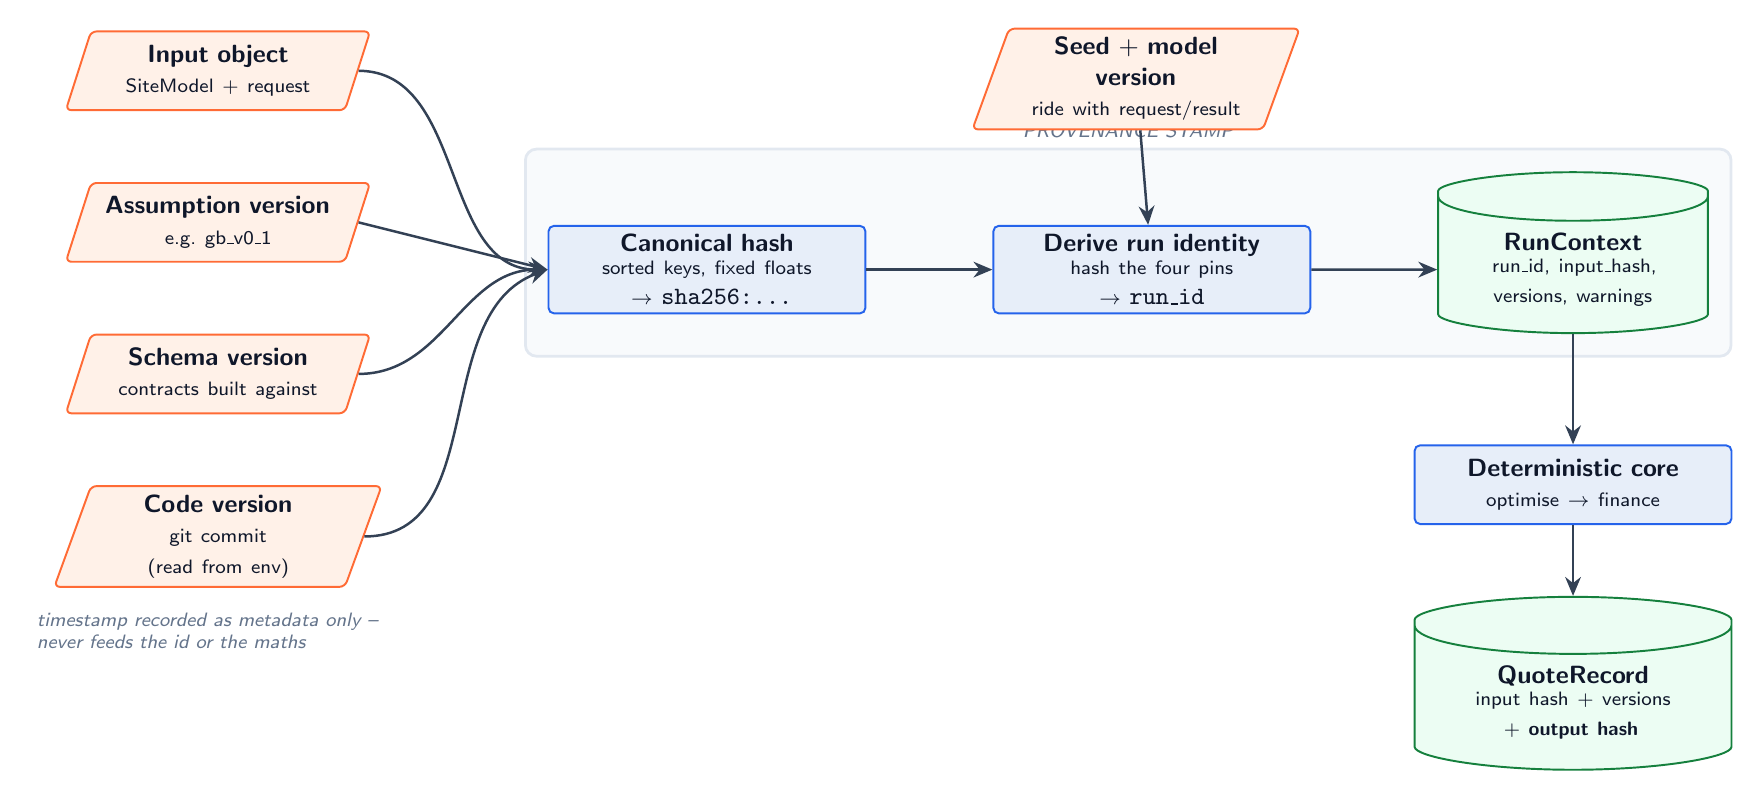
\begin{tikzpicture}[node distance=9mm and 16mm]
  % inputs feeding the hash
  \node[io] (input) {\textbf{Input object}\\\scriptsize SiteModel + request};
  \node[io, below=of input] (assum) {\textbf{Assumption version}\\\scriptsize e.g.\ gb\_v0\_1};
  \node[io, below=of assum] (schema) {\textbf{Schema version}\\\scriptsize contracts built against};
  \node[io, below=of schema] (code) {\textbf{Code version}\\\scriptsize git commit (read from env)};

  % canonical hashing stage
  \node[proc, right=24mm of assum, yshift=-6mm, minimum width=40mm, text width=38mm] (canon)
    {\textbf{Canonical hash}\\\scriptsize sorted keys, fixed floats\\\scriptsize $\rightarrow$ \code{sha256:\ldots}};

  \node[proc, right=of canon, minimum width=40mm, text width=38mm] (derive)
    {\textbf{Derive run identity}\\\scriptsize hash the four pins\\\scriptsize $\rightarrow$ \code{run\_id}};

  % seed + model side note
  \node[io, above=12mm of derive, xshift=-2mm] (seed) {\textbf{Seed} + \textbf{model version}\\\scriptsize ride with request/result};

  % run context store
  \node[store, right=of derive, minimum width=34mm, text width=32mm] (ctx)
    {\textbf{RunContext}\\\scriptsize run\_id, input\_hash,\\\scriptsize versions, warnings};

  % core run + quote record
  \node[proc, below=14mm of ctx, minimum width=40mm, text width=38mm] (core)
    {\textbf{Deterministic core}\\\scriptsize optimise $\rightarrow$ finance};
  \node[store, below=of core, minimum width=40mm, text width=38mm] (quote)
    {\textbf{QuoteRecord}\\\scriptsize input hash + versions\\\scriptsize + \textbf{output hash}};

  % arrows: inputs to canonical hash
  \draw[flow] (input.east) to[out=0,in=180] (canon.west);
  \draw[flow] (assum.east) -- (canon.west);
  \draw[flow] (schema.east) to[out=0,in=180] (canon.west);
  \draw[flow] (code.east) to[out=0,in=200] (canon.west);

  \draw[flow] (canon) -- (derive);
  \draw[flow] (seed) -- (derive);
  \draw[flow] (derive) -- (ctx);
  \draw[flow] (ctx) -- (core);
  \draw[flow] (core) -- (quote);

  % the timestamp is NOT an input
  \node[note, below=2mm of code, text width=46mm] {timestamp recorded as metadata only --\\ never feeds the id or the maths};

  % zone backdrop
  \begin{scope}[on background layer]
    \node[groupbox, fit=(canon)(derive)(ctx), inner sep=8pt,
          label={[note]north:PROVENANCE STAMP}] {};
  \end{scope}
\end{tikzpicture}}
\caption{How a run identity is made. The input is fingerprinted; the four pinned identifiers (input hash, assumption, code and schema versions) are hashed to derive a deterministic \code{run\_id}; the seed and engine model version ride alongside. The resulting \texttt{RunContext} stamps the deterministic core, whose output is sealed into the immutable \texttt{QuoteRecord} with an output hash. The wall-clock time is recorded but never feeds either the identity or the maths.}
\label{fig:provenance-identity}
\end{figure}

\section{Input hash and output hash: two fingerprints, two jobs}

A finished run carries two hashes, and it is worth being precise about which does which job, because they are easy to confuse.

The \textbf{input hash} is a fingerprint of everything fed in: the canonical hash of the site and request. It is a \emph{determinant}, one of the things that pins the answer. Change the input and this hash changes, and so, legitimately, may the result.

The \textbf{output hash} is a fingerprint of what came out: the canonical hash of the produced optimisation result and financial case. It is \emph{not} a determinant; nothing downstream is computed from it. Its job is to be a \emph{verifier}. The promise of determinism is that a re-run from the same pins reproduces the same output hash. So the output hash is the value a repro test checks: it is how you confirm, after the fact, that a re-run genuinely reproduced the original, rather than something that fed into producing it.

\begin{plainnote}
The input hash is the question's fingerprint; the output hash is the answer's fingerprint. The platform's guarantee is that the same question, asked the same way, always yields an answer with the same fingerprint. You verify a re-run by checking the answer's fingerprint, not by re-deriving it from the answer.
\end{plainnote}

Figure~\ref{fig:provenance-rerun} shows the verification in motion: the same five pins run a second time, on the same platform, and the output hash is compared against the one stored on the original record. A match is the determinism guarantee, demonstrated rather than asserted.

\begin{figure}[H]
\centering
\resizebox{0.92\textwidth}{!}{%
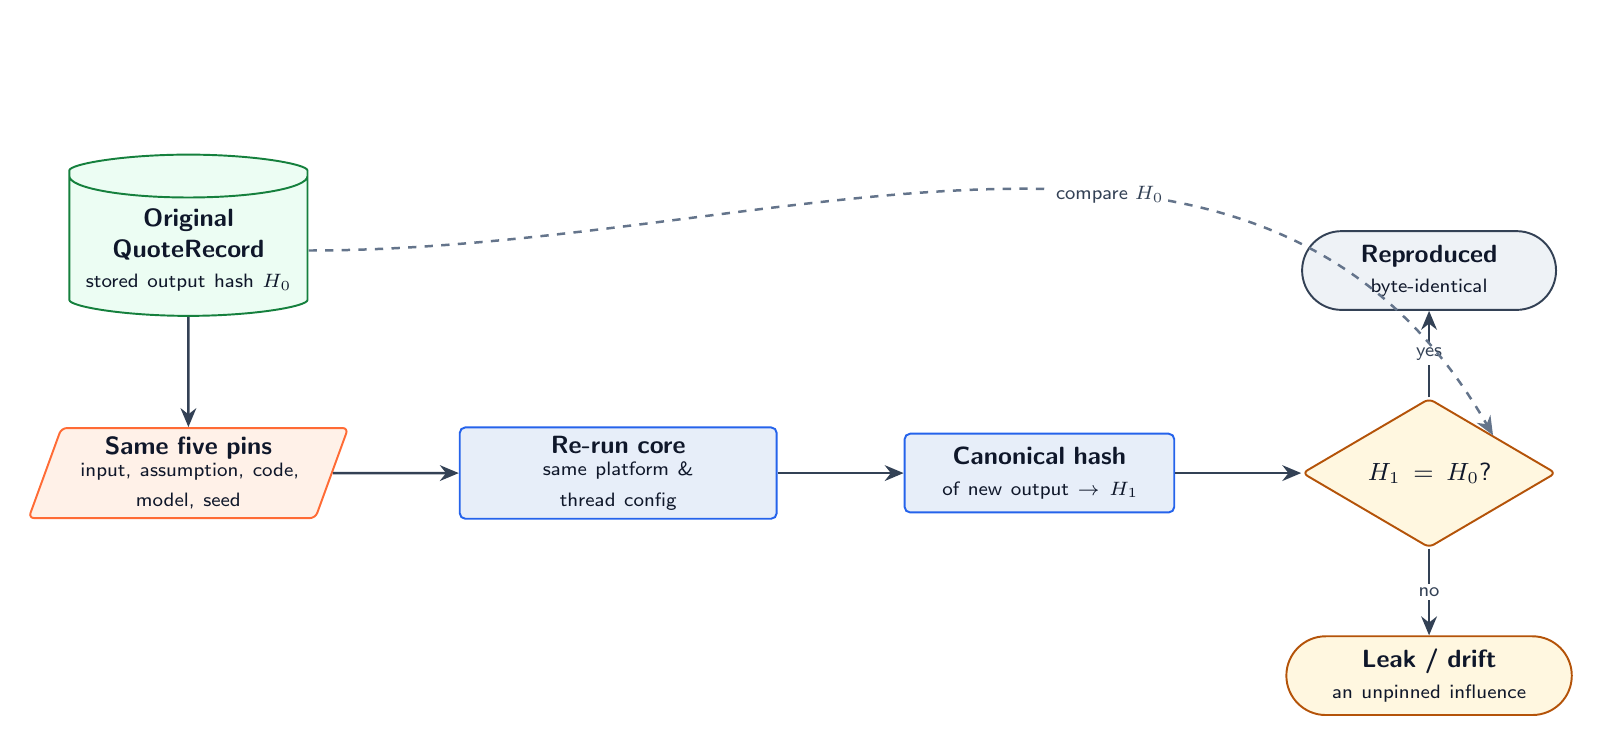
\begin{tikzpicture}[node distance=8mm and 16mm]
  \node[store] (orig) {\textbf{Original}\\\textbf{QuoteRecord}\\\scriptsize stored output hash $H_0$};
  \node[io, below=14mm of orig] (pins) {\textbf{Same five pins}\\\scriptsize input, assumption, code,\\\scriptsize model, seed};
  \node[proc, right=of pins, minimum width=40mm, text width=38mm] (rerun)
    {\textbf{Re-run core}\\\scriptsize same platform \&\\\scriptsize thread config};
  \node[proc, right=of rerun, minimum width=34mm, text width=32mm] (rehash)
    {\textbf{Canonical hash}\\\scriptsize of new output $\rightarrow H_1$};
  \node[decide, right=of rehash] (cmp) {$H_1 = H_0$?};
  \node[term, above=11mm of cmp, text width=30mm, minimum width=32mm] (ok)
    {\textbf{Reproduced}\\\scriptsize byte-identical};
  \node[term, below=11mm of cmp, draw=nodeDecisionBd, fill=nodeDecision, text width=34mm, minimum width=36mm] (bad)
    {\textbf{Leak / drift}\\\scriptsize an unpinned influence};

  \draw[flow] (orig) -- (pins);
  \draw[flow] (pins) -- (rerun);
  \draw[flow] (rerun) -- (rehash);
  \draw[flow] (rehash) -- (cmp);
  \draw[flow] (cmp) -- node[flowlabel]{yes} (ok);
  \draw[flow] (cmp) -- node[flowlabel]{no} (bad);
  \draw[flowback] (orig.east) to[out=0,in=120] node[flowlabel,pos=0.6]{compare $H_0$} (cmp.north east);
\end{tikzpicture}}
\caption{Reproduction as a test. The same five pins are re-run on the same platform; the new output is canonically hashed and compared with the hash stored on the original record. A match demonstrates determinism; a mismatch on the same platform means an unpinned influence (a leak) has reached the pricing path and must be removed.}
\label{fig:provenance-rerun}
\end{figure}

\section{Code version and model version stay orthogonal}

Two of the five pins both describe ``the software'', and keeping them separate is a deliberate and useful distinction.

\textbf{Code version} is the identity of the \emph{repository}: the git commit (or, failing a checkout, the package version) of everything that ran, the glue, the finance maths, the schema definitions. It moves whenever anyone commits a change.

\textbf{Model version} is the identity of the \emph{optimisation engine's own mathematics}: the name of the solver and the formulation it implements (for the integration-only baseline this is simply \code{mock}; a real engine would name its solver and formulation). It moves only when the engine's maths or solver actually change, even if a hundred unrelated commits land in between.

Holding the two on separate axes makes one question answerable that would otherwise be a guess: \emph{which change moved the number?} If a figure shifts and only the code version changed, the cause is somewhere in the surrounding software, not the optimiser; if only the model version changed, the optimiser's maths moved. Collapse the two into one ``version'' and you lose the ability to tell them apart, and with it the ability to attribute a change.

\begin{caution}[Same platform: byte-identical; across platforms: tolerance-equal]
Reproducibility has a sharp boundary that must be stated honestly. On the \emph{same} platform, the same five pins reproduce a \emph{byte-identical} output hash, and that is what the repro test asserts. \emph{Across} platforms the bar is weaker: floating-point results from BLAS-backed numerics and from the MILP solver can differ in their last bits with a different CPU architecture, thread count, or library build, so byte-identity is not promised across hosts. The guarantee there is numerical equality within a documented tolerance. To keep a cross-host mismatch diagnosable rather than alarming, each record also carries a \emph{reproduction-environment} tag (platform, architecture and solver mode), and the solver is pinned to deterministic, single-thread operation. The honest summary: byte-identical on the same platform, tolerance-equal across platforms.
\end{caution}

\section{Why the record must show the pins}

The reason every output, the underwriting memo, the proposal, and the quote record itself, must carry the assumption version and the input hash follows directly from the two guarantees:

\begin{itemize}
  \item \textbf{Reproducible.} With the input hash, the assumption version, the code and model versions and the seed, a lender's figure can be \emph{re-derived} on the same platform rather than taken on trust. A number that cannot be regenerated is not bankable.
  \item \textbf{Traceable.} The assumption version ties every figure to the exact values that produced it (and their recorded source, status and confidence, Chapter~\ref{ch:assumptions}); the input hash ties it to the exact site and request. Together they answer ``where did this come from'' precisely.
  \item \textbf{Valid only against its version.} A quote is valid only against the assumption version that produced it. If assumptions move beyond tolerance, the run reprices (a fresh, fully stamped snapshot) rather than drifting silently. This is the lifecycle rule made enforceable (Chapter~\ref{ch:quotes}).
\end{itemize}

\begin{rebuild}
To re-implement provenance from scratch, build the primitives first, then the stamp.
\begin{enumerate}
  \item \textbf{Canonical serialisation.} Write one function that renders any object to JSON deterministically: sort all keys, emit compact whitespace, and give every rich type one fixed rendering (dates and times to standard text; enumerated values to their stable value; decimals to exact text; sets sorted before writing; nested schema objects expanded the same way). Make an unhandled type a hard error, never a silent skip. \emph{Invariant:} two objects equal by value serialise to the identical string.
  \item \textbf{Hashing.} On top of that, expose an object hash (\code{sha256:} of the canonical string) and a file hash (\code{sha256:} of streamed bytes). Use these as the only fingerprinting tools anywhere.
  \item \textbf{Code version.} Read the git commit (short form, prefixed \code{git:}); fall back to the package version (\code{pkg:}) if there is no checkout. It must never raise.
  \item \textbf{Run context.} Given the input object, the assumption version and the schema version: hash the input; read the code version; hash the small object \{input hash, assumption version, code version, schema version\} in canonical form; take a short prefix of that digest as the \code{run\_id} (prefix it \code{run\_}). Attach the timestamp and warnings as metadata. \emph{Invariant:} the same pins always yield the same \code{run\_id}; the timestamp never feeds the id.
  \item \textbf{Fixed reduction order.} Anywhere floats are summed over a map (e.g. value-by-stream into a total), iterate in sorted-key order before accumulating, so the total is stable.
  \item \textbf{Output hash.} When the run completes, canonically hash the produced result and financial case; store it on the record as a verifier (never compute anything from it).
  \item \textbf{Keep code and model versions orthogonal.} Record both; let the engine name its own model version; never collapse them.
  \item \textbf{What to test.} A golden ``repro'' test: run an identical request twice on the same platform and assert the output hash is byte-identical. A canonical-form test: shuffle dictionary key order and confirm the hash is unchanged. A change-detection test: alter one input field and confirm the input hash changes. A clock-independence test: run at two different wall-clock times and confirm the \code{run\_id} and output hash are unchanged. Across platforms, assert numerical equality within the documented tolerance, not byte-identity.
\end{enumerate}
\end{rebuild}

\begin{keyidea}
Provenance turns trust into arithmetic. The output is a pure function of five pinned inputs; canonical serialisation and fixed reduction order make both hashes and totals stable; the run identity is derived from the pins, not the clock, so identical runs share an identity and re-runs are idempotent. The pins on the record let any number be re-derived and traced, which is precisely what makes it bankable.
\end{keyidea}

\chapter{The optimisation engine interface}
\label{ch:engine}

\modtag{Engine}{The optimisation engine interface}{Deterministic core, integration seam}

This chapter is about a boundary rather than a calculation. The platform's most expensive piece of mathematics is the optimiser that decides how big a battery a site should have and how it should charge and discharge through the year. That optimiser is genuinely hard to build. Everything that comes after it -- the financial model, the three documents, the web application -- is comparatively ordinary software. If the rest of the platform could only be built once the optimiser was finished, nothing would get built until everything got built, and the two would have to be tested together from day one.

The engine interface removes that dependency. It defines a thin, frozen contract: a precise description of what an optimiser is asked and what it must return, with no statement at all about how it computes the answer. Anything that honours the contract is, as far as the rest of the platform is concerned, ``the engine''. That lets the team build and test the entire pricing path against a deliberately fake optimiser -- a stand-in that returns the right \emph{shape} of answer with deliberately worthless \emph{numbers} -- and later swap in the real one without touching a single line of downstream code.

\begin{plainnote}
Think of a wall socket. An appliance does not know or care what is on the other side of the socket: a power station, a wind turbine, a diesel generator. It only relies on the shape of the plug and the voltage. The engine interface is that socket. Finance and the documents plug into it; behind it sits either a cheap mock or the real optimiser, and the appliance never notices the difference.
\end{plainnote}

\pipelinepos{receives the validated \textbf{SiteModel} (Ch.~\ref{ch:contracts}) and a versioned \textbf{assumption release} (Ch.~\ref{ch:assumptions}); hands an \textbf{OptimisationResult} to the financial model (Ch.~\ref{ch:finance})}

\section{Why the seam exists}

The platform is built by two people working in parallel. One owns the surrounding platform -- ingestion, schemas, assumptions, finance, the documents, the application. The other owns the optimiser proper: the value stack (Ch.~\ref{ch:valuestack}), the half-hourly dispatch solver (Ch.~\ref{ch:dispatch}), and the sizing search (Ch.~\ref{ch:sizing}). The engine interface is the single agreed line between those two bodies of work.

Because that line is frozen and small, the two halves do not need to meet constantly. They agree the shape of the request and the shape of the result once, and then each works independently against it. The platform half proves the whole pricing path runs end to end -- every document renders, every test passes -- while the optimiser half is still being written, because it runs against the mock. When the real optimiser is ready, the swap is the \emph{only} integration point, and it is guarded by an automated check (Section~\ref{sec:conformance}) rather than by a careful manual review.

\begin{keyidea}[One frozen line, two independent halves]
The seam is exactly two data shapes -- a request in, a result out -- plus the registry of value-stream names that travel inside them. Freeze those, and the optimiser and everything around it can be built, tested, and shipped on separate clocks. The mock-to-real swap becomes a single, automatically guarded event rather than a long, fragile merge.
\end{keyidea}

\begin{contract}
\textbf{Inputs} to the engine, per run:
\begin{itemize}
  \item a validated \textbf{SiteModel} -- the canonical site (load, connection, tariff, consents, counterparty);
  \item a loaded \textbf{assumption release} -- the single versioned source of every number, identified by its version tag;
  \item an optional \textbf{scenario-set identifier} -- which Low/Central/High case bundle to solve against (Ch.~\ref{ch:scenarios}).
\end{itemize}
\textbf{Outputs}:
\begin{itemize}
  \item an \textbf{OptimisationRequest} -- the assembled envelope the engine will solve (built from the three inputs above);
  \item an \textbf{OptimisationResult} -- the chosen battery size, the per-stream value, firmness flags, gated upside, solver status, and a provenance stamp. Its exact field list is the frozen contract in Ch.~\ref{ch:contracts}.
\end{itemize}
The engine \emph{never} writes a quote, never reads a file, never touches finance. It is a pure function from a request to a result.
\end{contract}

\section{The interface: two operations}

The contract is deliberately tiny. An engine is anything that offers two operations, in this order.

\begin{enumerate}
  \item \textbf{Build a request.} Given a SiteModel, an assumption release, and an optional scenario-set name, assemble the self-contained \emph{request envelope} the engine will then solve. The envelope bundles the site, the assumption version it is pinned to, the scenario set, the list of value streams to evaluate, and a flag naming which engine the request targets. Pinning the assumption version \emph{into} the request is what makes the run reproducible: the result can later be traced back to the exact numbers that produced it (Ch.~\ref{ch:provenance}).
  \item \textbf{Solve.} Given that request, return a schema-valid OptimisationResult.
\end{enumerate}

Two rules give the interface its strength and are worth stating plainly.

\begin{description}
  \item[An engine must not crash on thin data.] If a site is too sparse to size a system, the engine does not raise an error. It returns a perfectly valid result whose solver status says \code{insufficient\_data} and whose battery size is simply absent. This is the platform's ``degrade honestly'' principle (Ch.~\ref{ch:overview}) expressed at the engine boundary: the pipeline always gets an answer to consume, even when the answer is ``not enough information to size anything''.
  \item[An engine reports problems in the result, not by failing.] Warnings, binding constraints, and gate states all travel \emph{inside} the result as data. Downstream code reads them; it is never asked to catch an exception to learn that a stream could not be priced.
\end{description}

\begin{caution}[The interface is a Protocol, not a base class]
An engine does not inherit from anything. It simply \emph{has} the two operations with the right shapes. This is structural typing: the real optimiser, written in an entirely separate package, is an engine the moment it offers \code{build\_optimisation\_request} and \code{solve} with matching signatures. There is no shared parent to import, and therefore no hidden coupling between the platform and the optimiser beyond the two data shapes. It is implemented in the codebase as a runtime-checkable \fpath{Protocol} in \fpath{engine/interface.py}.
\end{caution}

\section{The integration-only baseline engine}

To build the platform before the optimiser exists, the team ships a fake engine that honours the interface and nothing more. It is called the \emph{baseline} engine, and its single job is to prove the plumbing: that a SiteModel can flow in, a result can flow out, finance can consume it, and the documents can render -- all end to end, with no real optimiser anywhere.

The baseline engine is built to be \emph{useless as economics and complete as plumbing}. Every result it returns carries two indelible flags: an implementation level of \code{baseline} and a bankable status of \code{not\_bankable}. It prices nothing: every value stream comes back at zero revenue and zero cost, marked excluded or, for the gated-upside streams, conditional. Its battery ``size'' is a crude placeholder -- a tenth of the site's peak import power, held for two hours -- computed by an in-code rule of thumb that is deliberately \emph{not} drawn from the assumption library, precisely so that no one can ever mistake it for a calibrated value.

\begin{caution}[Never read a baseline number as real]
The baseline figures are integration scaffolding, not advice. The ten-percent-of-peak sizing and the two-hour duration exist only to give the pipeline a non-empty shape to carry. The contract enforces the warning at the type level: a baseline-level result may never claim to be a bankable candidate, and the conformance suite (Section~\ref{sec:conformance}) has an explicit check that a baseline result is always \code{not\_bankable}. This is the ``never spoof a real engine'' guard.
\end{caution}

What the baseline engine does honestly is degrade. If a site has no usable peak-import figure, it cannot size even a placeholder, so it returns no size at all and sets its status to \code{insufficient\_data} with a plain warning saying why. That is the same honest-degradation behaviour the real engine must show, exercised here so the downstream code that handles ``no system'' is tested long before the real optimiser arrives.

\begin{table}[H]
\centering
\caption{What the baseline engine puts in every result, and why.}
\label{tab:baseline}
\small\sffamily
\begin{tabularx}{\textwidth}{@{}l L@{}}
\toprule
\textbf{Field} & \textbf{Baseline value and reason} \\
\midrule
Implementation level & \code{baseline} -- a permanent ``this is not a real engine'' marker. \\
Bankable status & \code{not\_bankable} -- enforced; a baseline result can never be a bankable candidate. \\
Selected size & A tenth of peak import power, held two hours; or absent when peak import is missing. \\
Value streams & Every requested non-gated stream at zero, marked \emph{excluded}, ``not priced yet''. \\
Gated upside & The three gated streams at zero, marked \emph{conditional}, each with a placeholder unlock condition. \\
Solver status & \code{baseline} when sized, \code{insufficient\_data} when peak import is missing. \\
Provenance stamp & Model version ``baseline'', plus the assumption and code versions of the run. \\
Warnings & Always state, in words, that this is plumbing only and not bankable. \\
\bottomrule
\end{tabularx}
\end{table}

\section{The seam at a glance}

Figure~\ref{fig:seam} is the whole boundary. The same request flows into one of two interchangeable engines -- the mock or the real optimiser -- and out comes a result whose \emph{shape} is identical either way. The conformance gate sits across the swap: it is the thing that lets the platform trust a freshly written real engine without re-testing everything downstream.

\begin{figure}[H]
\centering
\resizebox{\textwidth}{!}{%
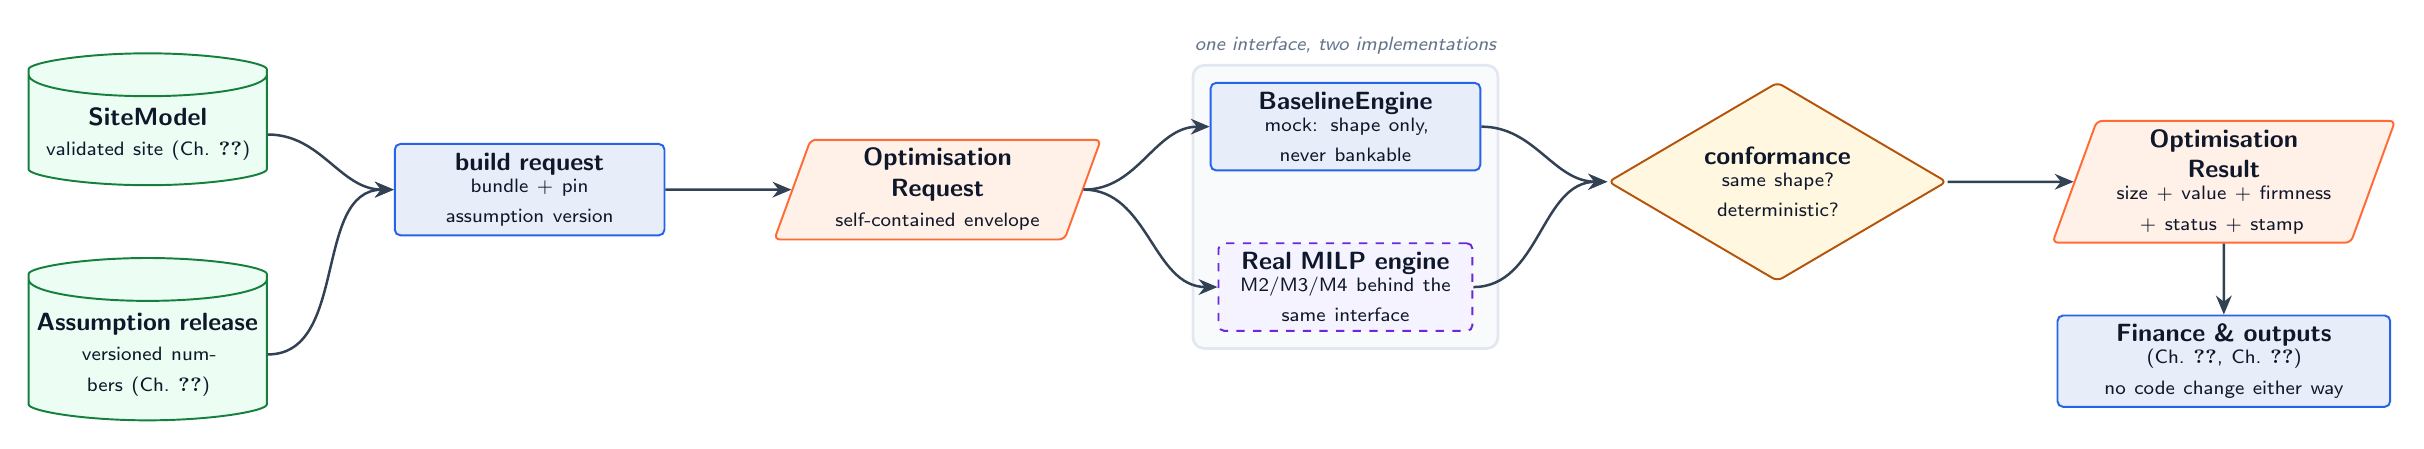
\begin{tikzpicture}[node distance=9mm and 16mm]
  % inputs
  \node[store] (site) {\textbf{SiteModel}\\\scriptsize validated site (Ch.~\ref{ch:contracts})};
  \node[store, below=of site] (assum) {\textbf{Assumption release}\\\scriptsize versioned numbers (Ch.~\ref{ch:assumptions})};

  % build request
  \node[proc, right=of site, yshift=-7mm] (build) {\textbf{build request}\\\scriptsize bundle + pin\\\scriptsize assumption version};
  \node[io, right=of build] (req) {\textbf{Optimisation\\Request}\\\scriptsize self-contained envelope};

  % the two interchangeable engines
  \node[proc, right=of req, yshift=8mm, draw=nodeProcessBd] (mock)
     {\textbf{BaselineEngine}\\\scriptsize mock: shape only,\\\scriptsize never bankable};
  \node[ext, below=of mock] (real)
     {\textbf{Real MILP engine}\\\scriptsize M2/M3/M4 behind the\\\scriptsize same interface};

  % conformance gate
  \node[decide, right=of mock, yshift=-7mm] (conf)
     {\textbf{conformance}\\\scriptsize same shape?\\\scriptsize deterministic?};

  % output + consumers
  \node[io, right=of conf] (res) {\textbf{Optimisation\\Result}\\\scriptsize size + value + firmness\\\scriptsize + status + stamp};
  \node[proc, below=of res, minimum width=42mm, text width=40mm] (fin)
     {\textbf{Finance \& outputs}\\\scriptsize (Ch.~\ref{ch:finance}, Ch.~\ref{ch:outputs})\\\scriptsize no code change either way};

  % arrows
  \draw[flow] (site.east) to[out=0,in=180] (build.west);
  \draw[flow] (assum.east) to[out=0,in=180] (build.west);
  \draw[flow] (build) -- (req);
  \draw[flow] (req.east) to[out=0,in=180] (mock.west);
  \draw[flow] (req.east) to[out=0,in=180] (real.west);
  \draw[flow] (mock.east) to[out=0,in=180] (conf.west);
  \draw[flow] (real.east) to[out=0,in=180] (conf.west);
  \draw[flow] (conf) -- (res);
  \draw[flow] (res) -- (fin);

  % grouping: the interchangeable engines sit behind one interface
  \begin{scope}[on background layer]
    \node[groupbox, fit=(mock)(real), inner sep=6pt,
          label={[note,anchor=south]north:one interface, two implementations}] {};
  \end{scope}
\end{tikzpicture}}
\caption{The engine seam. A request is built by pinning a SiteModel and an assumption release together, then solved by either the integration-only mock or the real MILP optimiser -- both behind one interface. The conformance gate guards the swap: it checks that the result has the same shape and is deterministic, not that the numbers match. Finance and the documents consume the result with no code change whichever engine produced it.}
\label{fig:seam}
\end{figure}

\section{Conformance: guarding the swap}
\label{sec:conformance}

The swap from mock to real engine is the platform's single riskiest moment. A subtly wrong real engine -- one that, say, returns a result on a slightly different schema, or labels a gated speculative stream as firm contracted income -- could poison every document downstream while every test still appeared green. The \emph{conformance suite} exists to make that impossible. It is an executable checklist that any engine, mock or real, must pass before it is trusted.

The single most important thing to understand about conformance is what it does \emph{not} check.

\begin{keyidea}[Conformance checks the contract, never the numbers]
The real optimiser will legitimately produce different battery sizes and different revenues than the mock -- that is the entire point of replacing the mock. So conformance never asserts that any number matches. It asserts that the result has the \emph{same schema}, uses the \emph{same stream vocabulary}, obeys the contract's invariants, and is \emph{deterministic}. Pass it, and the guarantee is: ``downstream needs no code change and stays reproducible'', not ``the answer is the same''.
\end{keyidea}

The suite runs in two layers. The first inspects a single result against the contract's invariants. The second drives a whole engine across a small set of representative sites and additionally checks determinism. Crucially, the suite depends only on the frozen contracts and the engine interface -- not on the platform or the test framework -- so the optimiser's author can run the \emph{exact same} checks against the real engine in its own package, with one line of code.

\begin{table}[H]
\centering
\caption{What the conformance suite actually checks. None of these is a numeric equality.}
\label{tab:conformance}
\small\sffamily
\begin{tabularx}{\textwidth}{@{}l L@{}}
\toprule
\textbf{Check} & \textbf{What it guarantees} \\
\midrule
Re-validates & The result survives a round trip through its own schema; no stray or mistyped fields. \\
Schema version pin & The result is on the frozen contract version, not a drifted one. \\
Run stamped & The result carries a non-empty engine, assumption, and code version -- it is traceable. \\
Request echo & The result names the request it answered, so finance can correlate the two by identity. \\
Registry membership & Every reported stream is a known name in the value-stream registry. \\
No duplicate streams & No stream is reported twice within a list, which would double-count in finance. \\
Gated-upside hygiene & Only the three gated streams appear in the gated list, and none is ever marked firm. \\
Gated never in the floor & A gated stream is never firm \emph{or} contracted, so it can never enter priced revenue. \\
Gated states its unlock & Each gated stream says, in words, what would let it be priced. \\
Baseline not bankable & A baseline-level result is always \code{not\_bankable} (the anti-spoof guard). \\
Sizing coherence & Power and energy travel together: both present, both zero, or both absent. \\
Status vs.\ spec & A no-solve status (infeasible or insufficient data) carries no battery size. \\
Determinism & Solving the same request twice gives the same result, ignoring wall-clock fields. \\
\bottomrule
\end{tabularx}
\end{table}

Several of these checks have ``teeth beyond the schema'' -- they catch drift the field-level validation alone would let through. The schema bars a gated stream from being \emph{firm}, but it would happily accept a gated stream labelled \emph{contracted}; conformance closes that gap, because a contracted gated stream would silently inflate the priced revenue floor. Likewise the schema only forbids a baseline result from claiming the strongest bankable label, while conformance forbids it from claiming \emph{any} bankable label. And the determinism check is something no single-result inspection could ever catch: it solves twice and compares.

\begin{plainnote}[Why determinism, not equality]
When comparing two solves of the same request, the suite ignores the fields that an honest engine is allowed to vary between runs without breaking reproducibility: the wall-clock timestamp, the measured solve time, the per-run identity tag, and the pointer to the off-contract dispatch schedule. Everything economic -- the size, the values, the firmness, the status, the versions -- must be byte-for-byte identical. That is the precise, testable meaning of ``the engine is deterministic''.
\end{plainnote}

The representative sites the suite drives an engine across are built from the schema itself, never hand-written, so they stay valid as the contract evolves. They cover three branches every engine must handle: a full validated site that should size cleanly, a partial site that should still size, and a coarse annual-only site with no peak-import figure that must trigger the insufficient-data path. An engine that raises an exception on any of these valid sites fails conformance: the suite records the exception as a failed check rather than letting it propagate, so a drifting engine shows \emph{all} its violations at once.

\section{The optional hooks a real engine may expose}

The frozen result deliberately carries only the headline economics: the chosen size and the per-stream value. The optimiser, however, computes far more along the way -- the full half-hourly dispatch, every sizing candidate it evaluated, the precise charge and discharge volumes. Some of that detail is useful downstream: finance needs the annual charge volume to apply levies, and the application wants to plot the sizing surface and a representative dispatch day. But none of it belongs \emph{on} the frozen result, because the mock cannot produce it and the contract must stay small.

The platform resolves this with \emph{optional hooks}. A real engine may expose three extra methods; the platform reads each one \emph{defensively}, so a mock that lacks them works exactly as before, with no downstream change. The pattern is uniform: ask the engine whether it offers the hook; if it does, use what it returns; if not, leave the corresponding detail absent and carry on honestly.

\begin{table}[H]
\centering
\caption{The three optional hooks, read defensively so a mock without them still works.}
\label{tab:hooks}
\small\sffamily
\begin{tabularx}{\textwidth}{@{}l L L@{}}
\toprule
\textbf{Hook} & \textbf{What it returns} & \textbf{What it feeds} \\
\midrule
Selected dispatch energy & The chosen system's annual charge and discharge volumes (kWh). & Finance's levies-on-charge and price-to-target lines (Ch.~\ref{ch:finance}); absent on the mock, so those lines stay honestly unavailable. \\
Full evaluated sizing grid & Every power-by-duration candidate the search evaluated, each with its return and covenant feasibility, plus the chosen optimum. & The 3D sizing surface in the application (Ch.~\ref{ch:sizing}, Ch.~\ref{ch:app}). \\
Representative dispatch day & One real solved day of half-hourly charge, discharge, state of energy, load, and price. & The dispatch chart in the application (Ch.~\ref{ch:dispatch}, Ch.~\ref{ch:app}). \\
\bottomrule
\end{tabularx}
\end{table}

\begin{caution}[Hooks are additive, never on the frozen seam]
The hooks live \emph{beside} the result, not inside it. Reading them defensively is what keeps the seam frozen: adding a hook to the real engine never changes the OptimisationResult shape, never trips conformance, and never forces a code change in any consumer that does not want the extra detail. The detail that the hooks expose carries no invented numbers either -- the sizing grid copies each candidate's real evaluated figures, and the representative day is one genuine solved day chosen deterministically, never an average or a synthesised shape.
\end{caution}

\begin{rebuild}[How to rebuild the engine seam]
\begin{enumerate}
  \item \textbf{Define the two data shapes first.} Freeze an \emph{OptimisationRequest} (site, pinned assumption version, scenario set, requested streams, target-engine flag) and an \emph{OptimisationResult} (chosen power/energy/duration, per-stream value with firmness, gated upside, binding constraints, solver status, a version stamp, warnings). Pin both to a schema version. Ship the value-stream name registry alongside them; an unknown stream name is a validation error, not a pass-through.
  \item \textbf{Declare the interface as a structural Protocol.} Two operations only: \emph{build a request} from (site, assumptions, optional scenario set), and \emph{solve} a request into a result. No base class. Require that solving never raises on a valid site; thin data is reported via the solver status and warnings.
  \item \textbf{Write the integration-only mock.} Have it build a request that asks for every stream, then return a result that is \emph{shape-complete and value-empty}: a placeholder size from an in-code rule of thumb (not from the assumption library), every stream at zero, implementation level \code{baseline}, bankable status \code{not\_bankable}, and a real provenance stamp. Make it degrade honestly: no peak-import figure means no size and an \code{insufficient\_data} status.
  \item \textbf{Write the conformance suite against the contracts only.} One layer of invariants on a single result (re-validates, schema-version pin, run stamped, request echo, registry membership, no duplicates, gated-upside hygiene, gated never in the priced floor, gated states its unlock, baseline-never-bankable, sizing coherence, status-vs-spec). One layer that drives an engine across schema-built representative sites (full, partial, annual-only) and solves twice to check determinism, ignoring only wall-clock and identity fields. Record raised exceptions as failures; never assert numbers.
  \item \textbf{Read the optional hooks defensively.} Where the platform wants engine detail beyond the result -- annual charge/discharge energy, the full sizing grid, a representative dispatch day -- ask the engine whether it offers the hook and use it only if present. A mock without the hook must leave the detail absent with no other change.
  \item \textbf{Test:} the mock passes conformance; a deliberately broken engine (drifted schema, a firm gated stream, a non-deterministic solve, a bankable baseline) fails the matching check; the full pipeline runs end to end on the mock; and switching to a real engine that passes conformance requires no edit to finance, outputs, or the application.
\end{enumerate}
\end{rebuild}

\begin{keyidea}[The one thing to remember]
The engine is reached only through a frozen request-in, result-out contract; the integration-only mock holds that contract today and is always \code{not\_bankable}; and a single, numbers-blind conformance suite lets the real optimiser drop in behind the same contract with no downstream change. The seam guarantees \emph{sameness of shape and reproducibility}, never sameness of answer.
\end{keyidea}

\chapter{The value and constraint stack}
\label{ch:valuestack}

\modtag{M2}{Value and constraint stack}{Deterministic core}

A battery on a commercial site does not earn money in one way. It can shave an expensive part of the electricity bill, it can be paid to stand ready in a national capacity scheme, it can deliver into a local network operator's flexibility tender, and -- once the right partner and permissions are in place -- it can trade in wholesale and balancing markets. Each of these is a separate \emph{income stream}, with its own rules about when it is allowed, how reliable it is, and how it is valued.

This module's job is to model all of those ways of earning as small, interchangeable pieces that the rest of the platform can treat identically. Every income stream is written behind one common shape: it can say what data it needs, decide whether it is available for this particular site, value itself against a proposed battery schedule, and declare the physical limits it places on that schedule. The core of the platform then handles a stream without ever knowing which market it belongs to.

\begin{plainnote}[The market is content, not code]
The single design rule of this module, taken verbatim from the platform brief, is that \emph{if the core ever has to ask ``is this Great Britain?'' the abstraction has failed}. Everything specific to the GB market -- which streams exist, which meter fields they read, which prices they use -- lives in one clearly-labelled content file and in the versioned assumption library (Chapter~\ref{ch:assumptions}). The generic machinery names no market at all. Adding a second country would mean writing a new content file, never editing the core.
\end{plainnote}

\pipelinepos{receives a validated \textbf{SiteModel} (Ch.~\ref{ch:contracts}) and the versioned \textbf{assumption library} (Ch.~\ref{ch:assumptions}); hands the dispatch optimiser (Ch.~\ref{ch:dispatch}) the value functions to maximise and the constraints to respect, and hands the finance model (Ch.~\ref{ch:finance}) a per-stream value-and-firmness breakdown.}

\begin{contract}
\textbf{In.} A validated \code{SiteModel} (tariff structure, connection limits, observed peak load, export consents, network region); the assumption library at a pinned version (the prices and factors each stream uses); a proposed battery \emph{dispatch schedule} to value (the charge/discharge plan from Ch.~\ref{ch:dispatch}); a \emph{scenario} carrying a price multiplier (Ch.~\ref{ch:scenarios}); and an optional, market-agnostic \emph{gate context} carrying three run-level facts the site data cannot hold.

\smallskip
\textbf{Out.} For each registered stream: a \code{GateResult} (is it available, and on what terms) and a per-stream \code{ValueStreamResult} carrying the annual revenue or cost, the stream's \emph{firmness}, its gate status, any unlock condition, the exact assumption keys used, and any not-bankable warnings. Plus a list of \emph{dispatch-constraint descriptors} naming the physical limits each stream imposes on the optimiser. Nothing here is a fabricated number: every figure is an assumption-library value multiplied by a quantity the dispatch schedule actually delivered.
\end{contract}

\section{The generic stream interface}

Every income stream, whatever it is, implements the same six-part interface. This is the contract the rest of the platform relies on, and it is the reason the core never special-cases a market.

\begin{table}[H]
\centering
\caption{The six things every value stream can do. The core calls these and nothing else.}
\label{tab:streamiface}
\small\sffamily
\begin{tabularx}{\textwidth}{@{}l L@{}}
\toprule
\textbf{Member} & \textbf{What it provides} \\
\midrule
\textbf{Identity} & A stable stream id from the frozen vocabulary, plus a human-readable display name for the documents. \\
\textbf{Required inputs} & The list of data items the stream needs to be assessed or priced. A missing item becomes a line on the site's ranked data ask, never a guess. \\
\textbf{Availability gate} & A deterministic check: given this site and these assumptions, is the stream open, conditional, closed, or undeterminable? (Section~\ref{sec:gates}.) \\
\textbf{Value function} & Given a battery dispatch schedule, the site, the assumptions and a scenario, the annual pounds the stream is worth. It values \emph{only} a schedule that is actually supplied. \\
\textbf{Constraints} & The physical limits the stream imposes on the optimiser, expressed as named descriptors that point at the field or assumption holding the binding number. \\
\textbf{Firmness and decay} & How reliable the stream's income is (Section~\ref{sec:firmness}), and, where relevant, how its capability erodes over the asset's life. \\
\bottomrule
\end{tabularx}
\end{table}

\subsection{Price and scenario inputs, kept at arm's length}

A value function is handed two objects whose internal shape it deliberately does not depend on: the dispatch schedule and the scenario. The dispatch schedule is the half-hourly charge-and-discharge plan produced by the optimiser (Chapter~\ref{ch:dispatch}); its full form is that module's to define. The scenario is the Low/Central/High price case from the scenario engine (Chapter~\ref{ch:scenarios}).

Rather than bind to either representation, a value function reads only the few \emph{aggregate quantities} it needs, by name. From the schedule it reads a small \emph{read model}: the sized battery's power (in megawatts) and storage duration (in hours), and a handful of optional delivered-energy figures (total annual discharge, discharge inside the network red-band windows, discharge inside an awarded local-flex tender's windows, and an engine-verified deliverable capacity). From the scenario it reads a single price multiplier, defaulting to one if the scenario does not supply it. This is the same loose coupling the finance model uses, and it lets the dispatch and scenario modules evolve their own data shapes without ever breaking the value stack.

\begin{keyidea}[One MWh is one decision, so double-counting is impossible]
The deepest invariant of the whole module: the battery follows \emph{one} dispatch schedule, and every stream is valued against that same schedule. A megawatt-hour discharged at 5pm is one decision the optimiser made once. The streams do not each get their own private battery to dispatch; they read the shared plan and price their slice of it. Because the schedule is singular, two streams cannot both claim the same energy. To make this watertight the customer-facing PPA/bill-savings stream -- the headline ``savings'' figure -- is deliberately priced at zero inside the stack, because its value is already itemised across the tariff-arbitrage, network-charge-avoidance and connection-headroom streams; counting it again would double-count the same avoided cost.
\end{keyidea}

\subsection{The versioned stream registry}

The streams a platform offers are held in a \emph{registry}: an ordered, id-keyed collection that the core consumes streams through. The registry is itself market-agnostic -- it simply holds whatever streams it was built with -- and it rejects duplicate ids so the set is unambiguous. A caller can ask for all streams, for a specific stream by id, or for the subset matching a requested list of ids (ids it does not know are simply skipped: the registry is the authority on what exists).

The current default registry is the GB value stack: nine streams, in the fixed order of the stream vocabulary. This ordered set is the ``versioned stream registry of valid stream ids'' the optimisation result contract refers to, and the same vocabulary that the contract tags (Ch.~\ref{ch:contracts}) and the contracted-versus-merchant split in finance (Ch.~\ref{ch:finance}) read against. A second market would supply its own builder function and wrap it in a registry of its own; the core would not change.

\section{Firm, contracted, conditional, excluded}
\label{sec:firmness}

Before any pounds are computed, each stream has a \emph{firmness}: how much a lender can rely on its income. Firmness is the property that decides whether a stream belongs in the \emph{priced floor} (the conservative income a deal is underwritten on) or is merely listed as upside. The four levels are summarised in Table~\ref{tab:firmness}.

\begin{table}[H]
\centering
\caption{The four firmness levels and how they map to a stream's gate.}
\label{tab:firmness}
\small\sffamily
\begin{tabularx}{\textwidth}{@{}l l L@{}}
\toprule
\textbf{Firmness} & \textbf{In the floor?} & \textbf{Meaning} \\
\midrule
\textbf{Firm} & Yes & Import-side savings that need no external partner: the gate is open and the data is present. \\
\textbf{Contracted} & Yes & Income that becomes contractual when its precondition holds (Capacity Market, local flexibility). In the floor only once that precondition is confirmed. \\
\textbf{Conditional} & No & Unlockable but a precondition is unmet. Listed as conditional upside with the exact condition that would unlock it. \\
\textbf{Excluded} & No & A required input is wholly absent; the stream cannot be assessed at all. \\
\bottomrule
\end{tabularx}
\end{table}

\begin{caution}[Firmness is not the same question as value]
``Will this stream be in the floor?'' (firmness) is kept strictly separate from ``what is it worth?'' (the pounds). The gate sets the firmness; the value function sets the number. A firm stream still reports zero pounds when no dispatch schedule is supplied (there is nothing to value yet). A conditional stream may carry a clearly-labelled upside figure -- for example a Capacity Market value computed before deliverability is confirmed -- but its conditional firmness keeps it out of the priced floor regardless. The finance floor counts only streams whose firmness is firm or contracted.
\end{caution}

The three categories of stream differ only in the firmness an \emph{open} gate implies. Floor streams open to firm; contracted streams open to contracted; gated-upside streams can never open at all (the best they reach is conditional). This is enforced structurally, in three independent places, so a speculative stream cannot slip into the bankable floor by accident: the gated-upside base class refuses to report an open gate, and both the gate-result and the per-stream-result validators reject any gated stream marked firm.

\section{How the availability gate works}
\label{sec:gates}

A stream's gate is a \emph{pure, deterministic} function of the site model and the assumption library: no randomness, no wall-clock time, no invented value. It returns one of four statuses, and a single shared builder turns that status into a consistent result so a stream can never report a contradictory (status, firmness) pair.

\begin{table}[H]
\centering
\caption{The four gate statuses and what each implies.}
\label{tab:gatestatus}
\small\sffamily
\begin{tabularx}{\textwidth}{@{}l l l L@{}}
\toprule
\textbf{Status} & \textbf{Priceable now?} & \textbf{Implied firmness} & \textbf{When it is reported} \\
\midrule
\textbf{Open} & Yes & firm or contracted & Every required input is present; the stream enters the priced floor. \\
\textbf{Conditional} & No & conditional & Unlockable, but a precondition is unmet; carries an unlock condition. \\
\textbf{Closed} & No & excluded & A required input is wholly absent; the stream cannot be assessed. \\
\textbf{Unknown} & No & excluded & The gate could not be determined; treated conservatively as excluded. \\
\bottomrule
\end{tabularx}
\end{table}

The builder enforces the mapping: a result is priceable \emph{if and only if} its status is open; a non-open gate can never be firm; an open gate can never be excluded; a conditional gate must always carry the condition that would unlock it. These checks live in exactly one place, so the rest of the code cannot get the pairing wrong.

\subsection{Gate predicates read only the site's own data}

The gates themselves are built from small market-agnostic predicates -- ``does the tariff have a usable price spread to arbitrage?'', ``is there network red-band rate data?'', ``is a connection limit recorded?'', ``is there an observed peak?'', ``are export consents approved and is export capability greater than zero?'' Each predicate reads the site's own fields and reports what is present or missing. Critically, a predicate that lacks its input returns \emph{false} -- producing a missing-requirement line -- never a guessed \emph{true}. The GB content file simply wires each predicate to the right meter field and assumption section.

\subsection{Three facts the site model cannot hold}

Three things a gate may need are not the site's own data, so they do not belong on the frozen site model: whether the battery's \emph{de-rated deliverability} holds to the final contract year at end-of-life capability (this is derived by the sized engine), whether a \emph{local-flexibility tender} is currently open in the site's network region (time-varying external market state), and the \emph{aggregated portfolio power} a fleet-level stream needs (a single-site run has none). These three flow in through a separate, generic \emph{gate context} object. Every field of it defaults to ``unknown'', so calling a gate with no context behaves identically to the data-only case: the affected streams stay conditional. This is generic run context the core threads through unread; it is not a market branch and not an assumption-library value.

\subsection{Pricing a stream out, and listing it as conditional upside}

When a gate's precondition fails -- a consent is not approved, metering is too thin to show a peak, or a portfolio is below the threshold for a fleet stream -- the stream is \emph{priced out of the floor}. It is not silently dropped. The gate reports a conditional (or closed) status, attaches the precise \code{missing\_requirements} that blocked it, and, for a conditional stream, an \code{unlock\_condition} stating exactly what would let it in: ``a route-to-market partner and approved export consents'', say, or ``a local-flex tender open in the site's network area plus a contracted award''. That list of unlock conditions is what the proposal and underwriting pack present as the deal's conditional upside, and it feeds the ranked data ask that tells the customer which missing item would most improve the quote.

\begin{figure}[H]
\centering
\resizebox{\textwidth}{!}{%
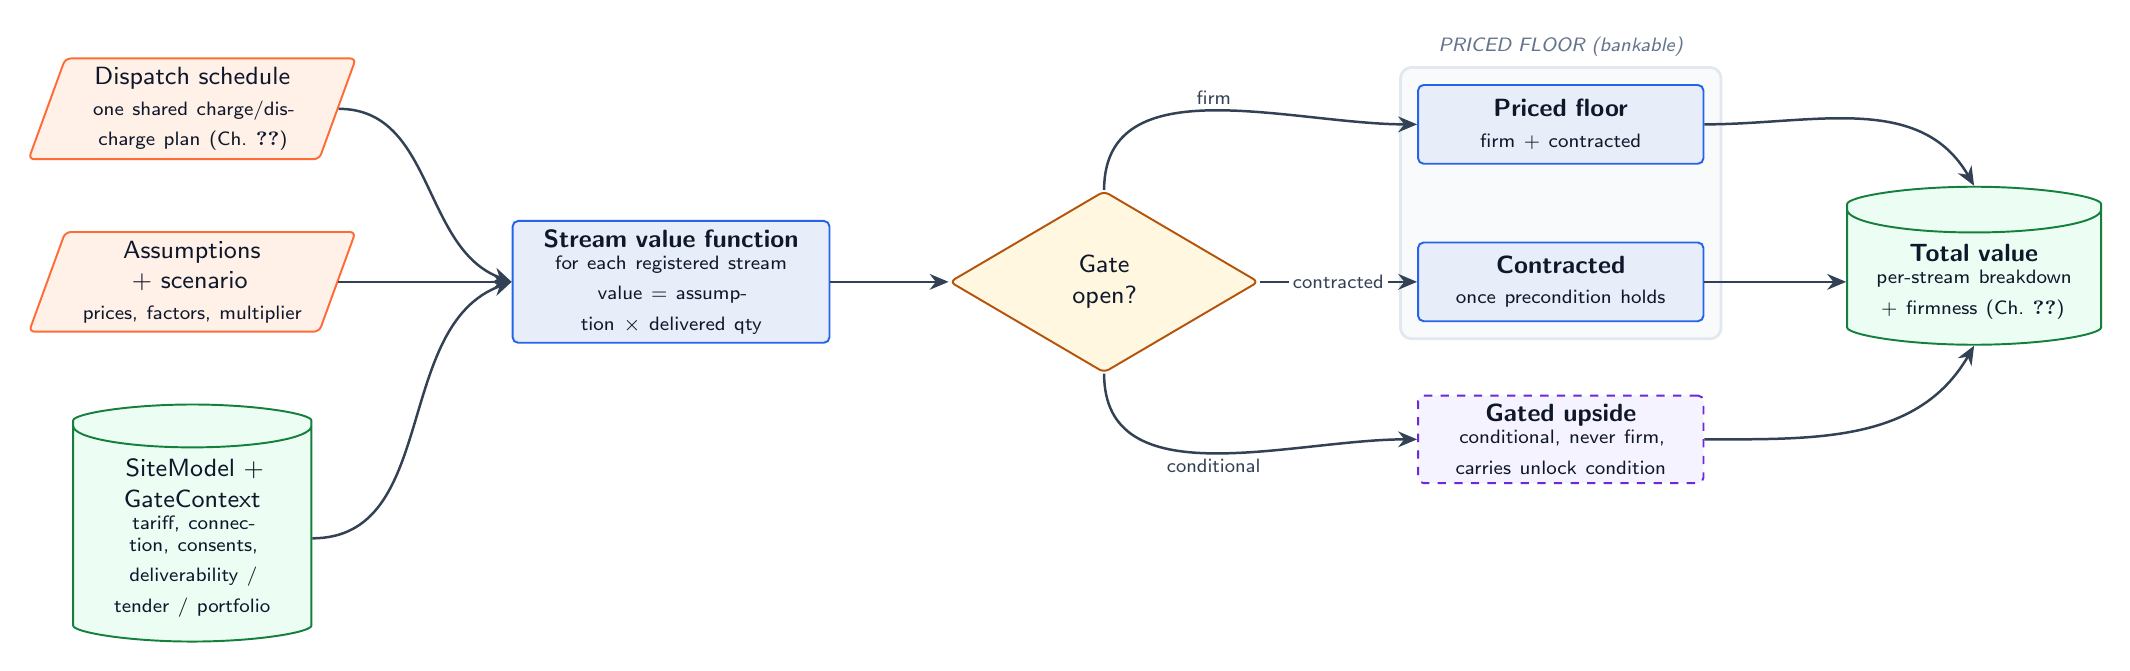
\begin{tikzpicture}[node distance=9mm and 15mm]
  % inputs
  \node[io] (sched) {Dispatch schedule\\\scriptsize one shared charge/discharge plan (Ch.~\ref*{ch:dispatch})};
  \node[io, below=of sched] (assum) {Assumptions + scenario\\\scriptsize prices, factors, multiplier};
  \node[store, below=of assum] (site) {SiteModel + GateContext\\\scriptsize tariff, connection, consents,\\\scriptsize deliverability / tender / portfolio};

  % the per-stream value function (one shown; applied to every registered stream)
  \node[proc, right=22mm of assum, minimum width=40mm, text width=38mm] (vf)
     {\textbf{Stream value function}\\\scriptsize for each registered stream\\\scriptsize value = assumption $\times$ delivered qty};

  % gate
  \node[decide, right=of vf] (gate) {Gate\\open?};

  % three buckets
  \node[proc, right=20mm of gate, yshift=20mm, text width=34mm] (floor)
     {\textbf{Priced floor}\\\scriptsize firm + contracted};
  \node[proc, right=20mm of gate, text width=34mm] (contracted)
     {\textbf{Contracted}\\\scriptsize once precondition holds};
  \node[proc, right=20mm of gate, yshift=-20mm, dashed, draw=nodeExtBd, fill=nodeExt, text width=34mm] (upside)
     {\textbf{Gated upside}\\\scriptsize conditional, never firm,\\\scriptsize carries unlock condition};

  % sum
  \node[store, right=18mm of contracted, text width=30mm] (total)
     {\textbf{Total value}\\\scriptsize per-stream breakdown\\\scriptsize + firmness (Ch.~\ref*{ch:finance})};

  % arrows in
  \draw[flow] (sched.east) to[out=0,in=160] (vf.west);
  \draw[flow] (assum.east) -- (vf.west);
  \draw[flow] (site.east) to[out=0,in=200] (vf.west);

  \draw[flow] (vf) -- (gate);

  % gate to buckets
  \draw[flow] (gate.north) to[out=90,in=180] node[flowlabel,above]{firm} (floor.west);
  \draw[flow] (gate.east) -- node[flowlabel]{contracted} (contracted.west);
  \draw[flow] (gate.south) to[out=-90,in=180] node[flowlabel,below]{conditional} (upside.west);

  % buckets to total
  \draw[flow] (floor.east) to[out=0,in=120] (total.north);
  \draw[flow] (contracted.east) -- (total.west);
  \draw[flow] (upside.east) to[out=0,in=240] (total.south);

  % grouping the priced floor
  \begin{scope}[on background layer]
    \node[groupbox, fit=(floor)(contracted), inner sep=6pt,
          label={[note,anchor=south]north:PRICED FLOOR (bankable)}] {};
  \end{scope}
\end{tikzpicture}}
\caption{One shared dispatch decision feeds every stream's value function. Each stream passes through its availability gate, which sorts it into the priced floor (firm or contracted), or lists it as gated upside with an unlock condition. The slices sum to a per-stream breakdown the finance model reads. Because all streams price the same single schedule, no megawatt-hour can be counted twice.}
\label{fig:valueflow}
\end{figure}

\section{The three buckets of streams}

The nine GB streams fall into three categories. Their gates and value formulas are the only GB-specific content; the categories themselves are generic.

\subsection{The bankable floor (priced, firm)}

These are the import-side savings the site captures without any external partner. Their gate opens to \emph{firm} the moment the necessary site data is present.

\begin{itemize}
  \item \textbf{Tariff arbitrage} -- buying cheaply and discharging when the supply rate is high. The gate needs a multi-rate import tariff (at least two distinct price points: a single flat rate has no spread to arbitrage) and load data. Valued, indicatively, as a per-megawatt-year figure times the sized power.
  \item \textbf{Network red-band avoidance} -- avoiding the most expensive distribution-use-of-system charges by not importing during the network's red-band windows. (This is the post-reform treatment; there is no Triad story.) The gate needs the red-band rate data and load.
  \item \textbf{Connection-headroom value (MIC/ASC)} -- the worth of staying within the site's agreed import and supply capacity, charged only where the connection actually binds the dispatch. The gate needs a recorded connection limit and an observed peak; an annual-only (coarse-tier) site has no peak, so the gate closes honestly.
  \item \textbf{PPA / bill savings} -- the customer-facing headline. Priced at \emph{zero} inside the stack on purpose, because its value is the sum of the three streams above; the customer price-per-unit is set later by the finance layer.
\end{itemize}

\begin{caution}[Avoiding the expensive red band and staying inside the connection]
Two of the floor streams are really about \emph{not} paying costs. Discharging across the network's red-band windows avoids the priciest distribution charges, and keeping import below the agreed maximum import and supply capacity (MIC/ASC) avoids penalties and reinforcement. Both are modelled as constraints on the optimiser (windows the battery must discharge into; a charge limit the battery must not breach) and as value the stream books only where the limit actually binds. The battery's own charging load counts against the import connection, so the optimiser is told the charge power is capped at the binding limit -- the lower of the import and supply capacities.
\end{caution}

\subsection{Contracted streams (priced once they hold)}

These become contractual revenue when a precondition is confirmed, and sit at conditional until then.

\begin{itemize}
  \item \textbf{Capacity Market} -- payment for standing ready to deliver in a national capacity scheme. The asset's contribution is \emph{de-rated} by its storage duration (a longer-duration battery counts for more), and it must hold that de-rated capacity in every contract year at end-of-life capability, sized day-one with no later augmentation. The deliverability fact arrives via the gate context; until it is confirmed the stream is conditional. Valued as a clearing price (pounds per kilowatt-year) times the de-rated capacity, where the de-rated figure is the engine-verified deliverable capacity if supplied, otherwise the sized power times the duration-based de-rating factor, with the annual capacity-fade percentage surfaced as the decay that erodes capability over life.
  \item \textbf{Local flexibility} -- delivering into a distribution network operator's flexibility tender (Piclo and similar). The gate needs the site's network region (to match a tender) and, via the gate context, an open tender plus a contracted award. Valued as a utilisation price (pounds per megawatt-hour) times the energy delivered inside the awarded tender windows.
\end{itemize}

\subsection{Gated upside (never in the floor)}

These three streams can be very valuable, but they can never be \emph{firm} and never enter the priced floor. They live in a separate ``gated upside'' list on the result, not among the priced streams.

\begin{itemize}
  \item \textbf{Wholesale and balancing via P415} -- trading energy and offering into the balancing mechanism through the P415 retail-energy-market arrangement. Unlocks only with a confirmed route-to-market partner and approved export consents (the export permissions G99/G100).
  \item \textbf{Balancing Mechanism} -- direct balancing-market participation. Unlocks with a route-to-market partner plus an aggregated portfolio above a minimum threshold (a single site is too small).
  \item \textbf{Ancillary services (DC/DM/DR)} -- the frequency-response products, whose value decays over the asset's life. Unlocks with a route-to-market partner and a portfolio above threshold.
\end{itemize}

\begin{caution}[Why the gated streams price to zero today]
The route-to-market partner is not yet known, so the assumption-library values for these three streams are deliberately a confirmed-status placeholder of \emph{zero}. The ``route-to-market available'' predicate returns true only when its assumption is both \emph{confirmed} and \emph{positive}, so on today's placeholders the streams stay conditional upside and price at exactly zero. The de-rating and decay machinery is fully wired and will activate unchanged the moment a real positive value lands -- by a version bump to the assumption library, not a code edit. This is how a placeholder can never masquerade as a bankable number.
\end{caution}

\section{Valuing a schedule without inventing revenue}

The value function never fabricates money. It prices a stream \emph{only} over a dispatch schedule that is actually supplied, and only ever as an assumption-library number multiplied by a quantity that schedule delivered. With no schedule, or with a closed or excluded gate, the stream reports zero pounds plus an explanatory note. Every priced figure carries a loud not-bankable warning naming the exact assumption key it used and that key's status, because on the current placeholder assumption set (\code{gb\_v0\_1}) every value is a stand-in. A scenario price multiplier other than one is applied and noted. The order of operations inside the value function is fixed:

\begin{enumerate}
  \item Run the gate to obtain the real firmness and status. This always happens, schedule or not.
  \item If there is no schedule, or the gate is closed or unknown, return a revenue-free result carrying the real firmness and a note. Stop.
  \item Otherwise read the schedule into the small aggregate read model. If it cannot be read, return revenue-free with a warning. Never invent the quantities.
  \item Compute the pounds: assumption value times the delivered quantity times the scenario multiplier. Attach the not-bankable warning naming the key, the assumption keys used, and any decay or conditional-upside note.
\end{enumerate}

\section{Constraints the streams impose on the optimiser}

A stream does not only earn value; it constrains how the battery may be dispatched. Each stream declares its limits as \emph{descriptors}: a stable id, a human description, a constraint family (connection limit, throughput cap, availability window, held state-of-energy, export limit, deliverability), and a pointer to the site field or assumption key that holds the binding number. The descriptors carry \emph{no} fabricated values: the actual numbers are read from the site model or assumptions at solve time. Examples include the connection charge limit (charge power capped at the lower of import and supply capacity), the warranty throughput cap (annual full-cycle-equivalents are hard-limited; the optimiser may not over-cycle), the red-band discharge window, the Capacity Market deliverability and held-energy-band constraints, the local-flex tender window, and the export limit. The dispatch optimiser (Chapter~\ref{ch:dispatch}) reads these descriptors and applies the global physics (round-trip losses, parasitic load, warranty caps) engine-wide.

\begin{rebuild}[How to rebuild this module]
\begin{enumerate}
  \item \textbf{Define the interface.} A value stream exposes: a stable id and display name; a list of required inputs (key, description, whether it blocks pricing); a deterministic \code{check\_gates(site, assumptions, context)} returning a gate result; a \code{value\_function(schedule, site, assumptions, scenario, context)} returning a per-stream result; and a \code{constraints(site, assumptions)} returning constraint descriptors.
  \item \textbf{Define the gate result and its invariants.} Fields: stream id, status (open/conditional/closed/unknown), priceable-now flag, firmness, missing-requirements list, optional unlock condition, warnings. Validate, in one builder: priceable iff open; non-open is never firm; open is never excluded; a gated-upside id is never firm; a conditional gate must carry an unlock condition.
  \item \textbf{Write the gate predicates market-agnostic.} Pure functions over the site model and assumption \emph{status} that return false (a missing requirement) when their input is absent -- never a guessed true. No market name appears.
  \item \textbf{Add the generic gate context.} A small object with three optional, default-unknown fields: deliverability confirmed, tender open, portfolio MW and its threshold. A \code{None} context must reproduce data-only behaviour exactly.
  \item \textbf{Build three category base classes.} Floor (open $\Rightarrow$ firm), contracted (open $\Rightarrow$ contracted), gated-upside (refuses an open gate; restricted to the gated ids). Each holds a revenue-free default value function that prices nothing.
  \item \textbf{Write the dispatch read model.} A structural shape exposing power, duration, and optional delivered-energy and deliverable-capacity figures, plus a normaliser that turns any duck-typed schedule into it or raises a read error (the caller then prices nothing).
  \item \textbf{Put the market content in one file.} The concrete streams: wire each gate predicate to the right field, override the value function with the formula (assumption value $\times$ delivered quantity $\times$ scenario multiplier), and attach a not-bankable warning naming the assumption key. No market branch anywhere else.
  \item \textbf{Register the streams.} An ordered, id-keyed registry rejecting duplicate ids, with a default-registry composition root assembling the market's stream set.
  \item \textbf{What to test.} Protocol conformance; the registry returns the expected streams; the gate-result invariants hold; gated streams can never be firm and price zero on placeholders; no schedule or a closed gate yields zero pounds; the gate context opens and prices Capacity Market and local flex and is additive; the same inputs always produce the same output (determinism); and no two streams can claim the same delivered energy.
\end{enumerate}
\end{rebuild}

\begin{keyidea}[What to remember]
Every way a battery earns money is one small object behind one generic interface, so the core never special-cases a market. A gate decides each stream's firmness and sorts it into the priced floor (firm or contracted), or lists it as conditional upside with an explicit unlock condition. Value is only ever an assumption-library number times a quantity the single shared dispatch schedule delivered, so no figure is invented and no megawatt-hour is counted twice.
\end{keyidea}

\chapter{The half-hourly dispatch optimiser}
\label{ch:dispatch}

\modtag{M3}{Half-hourly dispatch optimiser}{Deterministic core}

This is the calculation at the very centre of the platform. Everything before it prepares the ground -- a validated site, a versioned set of numbers, a list of income streams to consider -- and everything after it merely arranges the answer into documents. The dispatch optimiser is the part that actually decides what the battery \emph{does}: in each half hour of the year, does it charge, does it discharge, or does it sit still, and by how much? The sum of those decisions is the value the battery earns, and the value is the whole reason the project exists.

The decision is not obvious, because the battery is fighting on several fronts at once. Electricity is cheaper at some times of day than others, so the battery wants to fill up when power is cheap and empty out when it is dear. But charging draws power through the same grid connection the site already uses, and that connection has a hard ceiling; pushing past it is not allowed. The battery loses a little energy on every round trip, so a charge-and-discharge cycle only pays if the price gap more than covers the loss. The manufacturer's warranty caps how hard the battery may be cycled in a year. And the battery can only hold so much, and can never hold less than nothing. The optimiser must respect every one of these limits simultaneously and still find the single best pattern of charging and discharging.

\begin{plainnote}
Picture a tank of water with a pump that can fill it or drain it, a meter that charges you a different price each half hour for water you move, and a set of rules: the pipe is only so wide, a little water leaks out on every fill-drain cycle, and the pump's warranty allows only so many full cycles a year. Your job is to decide, for every half hour of the year, how much to pump in or out so that you save the most money on your water bill without breaking any rule. That is exactly the problem the dispatch optimiser solves -- only with electricity, and with the bill computed from the site's own tariff.
\end{plainnote}

\pipelinepos{receives the validated \textbf{SiteModel} (Ch.~\ref{ch:contracts}), a versioned \textbf{assumption release} (Ch.~\ref{ch:assumptions}), and the per-stream \textbf{gates and constraints} from the value stack (Ch.~\ref{ch:valuestack}); is called once per candidate size by the \textbf{sizing search} (Ch.~\ref{ch:sizing}); hands a \textbf{half-hourly schedule, per-stream value, and annual energy volumes} back through the engine seam (Ch.~\ref{ch:engine}) to finance (Ch.~\ref{ch:finance}).}

\section{What a mixed-integer linear program is}

The tool the optimiser uses is a \emph{mixed-integer linear program}, or MILP. The name unpacks into three plain ideas.

\begin{description}
  \item[Linear.] Every relationship in the model is a straight-line one: a quantity added to another quantity, or a quantity multiplied by a fixed number. The energy bought is the power drawn multiplied by the half-hour length; the bill is each half-hour's price multiplied by the energy moved, all summed up. There are no curves, no quantities multiplied by other unknown quantities. Linear models are valuable precisely because a solver can find their exact best answer reliably and fast.
  \item[Program.] An old word for ``optimisation problem'': a thing to be maximised or minimised, subject to a list of limits.
  \item[Mixed-integer.] Some of the decisions may be forced to whole numbers (on or off, one unit or two) rather than any fraction. Pure continuous dispatch -- how many kilowatts to charge -- needs no whole-number decisions, but the framework allows them, which is why the engine is described as a MILP and uses an integer-capable solver. In this engine the live decisions are continuous; the integer capability is held in reserve.
\end{description}

So a MILP is: \emph{choose values for a set of decision variables, some possibly whole numbers, to make a linear measure of value as large as possible, while never violating a list of linear limits.} The optimiser states the battery problem in exactly that form and hands it to a solver, which returns the provably best dispatch.

\begin{keyidea}[Maximise value, subject to physics]
The dispatch problem is one sentence: choose how much to charge and discharge in every half hour so the site's electricity bill falls as far as possible, subject to the grid connection, the battery's size, its round-trip losses, and its warranty cycle limit. The MILP is just a precise, solvable way of writing that sentence down. Because the maths is linear and the solver is deterministic, the same site and the same assumptions always yield the same schedule.
\end{keyidea}

\begin{contract}
\textbf{Inputs} to one dispatch solve:
\begin{itemize}
  \item a \textbf{fixed system spec} -- the battery's power (kW), energy (kWh), and duration (hours). The optimiser is \emph{told} the size; it does not choose it (that is the sizing search, Ch.~\ref{ch:sizing}).
  \item the \textbf{SiteModel} -- above all the half-hourly metered import series, the connection limits (MIC and ASC), and the tariff stack (time-of-use energy rates and DUoS band rates);
  \item the \textbf{assumption release} -- the round-trip efficiency and the warranty cycle table (no private constants live in the code);
  \item the \textbf{constraint descriptors} the value stack attaches to the requested streams (Ch.~\ref{ch:valuestack}) -- labels naming which limits apply, with no numbers baked in.
\end{itemize}
\textbf{Outputs}:
\begin{itemize}
  \item a \textbf{half-hourly schedule} -- charge, discharge, and state of energy for every metered half hour, plus the price signal optimised against;
  \item \textbf{value by stream} -- the annual revenue attributed to each income stream, with its firmness flag and gate state;
  \item \textbf{annual energy volumes} -- the year's total charge and discharge in kWh, and the equivalent full cycles, handed to finance;
  \item a \textbf{solver status} and a list of which constraints actually bound.
\end{itemize}
The solver \emph{never raises} on a valid site: thin data is reported through the status and warnings, never by crashing.
\end{contract}

\section{The decision variables: what the optimiser chooses}

For each half hour $t$ across the metered horizon, the optimiser controls three quantities. Let $\Delta t$ be the length of a half hour in hours (so $\Delta t = 0.5$ for half-hourly data; the engine derives it from the meter's interval rather than assuming it).

\begin{table}[H]
\centering
\caption{The three decision variables, defined for every half hour of the horizon.}
\label{tab:vars}
\small\sffamily
\begin{tabularx}{\textwidth}{@{}l l L@{}}
\toprule
\textbf{Variable} & \textbf{Unit} & \textbf{Meaning} \\
\midrule
charge$_t$ & kW & The power drawn from the grid into the battery during half hour $t$. \\
discharge$_t$ & kW & The power delivered from the battery to the site's load during half hour $t$. \\
soe$_t$ & kWh & The state of energy: how much usable energy sits in the battery at the end of half hour $t$. \\
\bottomrule
\end{tabularx}
\end{table}

These are powers (kW) on the AC side -- the side the grid meter sees -- not energies. The energy moved in a half hour is the power multiplied by $\Delta t$. Charge and discharge are kept as two separate non-negative variables rather than one signed quantity, which lets the model treat their limits and their efficiency loss cleanly and keeps the schedule free of any half hour that pretends to charge and discharge at once.

\section{The constraints: the limits the schedule must respect}

The constraints are what separate a real dispatch from a fantasy one. Each is a linear rule that must hold in every half hour (or, for the cycle cap, across the whole horizon).

\subsection{State-of-energy dynamics and round-trip losses}

The battery's stored energy is a running total. Whatever was in the battery at the end of the previous half hour, plus what charging added, minus what discharging removed, is what remains now:
\[
\text{soe}_t \;=\; \text{soe}_{t-1} \;+\; \text{charge}_t \cdot \text{RTE} \cdot \Delta t \;-\; \text{discharge}_t \cdot \Delta t .
\]
Here \textbf{RTE} is the round-trip efficiency, a number between 0 and 1 read from the assumption library (\code{\seqsplit{round\_trip\_efficiency.ac\_round\_trip}}). It captures the energy lost on a full charge-and-discharge cycle: charging adds only the RTE fraction of the grid energy to the store, while discharging removes energy at face value. The arithmetic consequence is exact and important: over the year, \emph{total grid charge equals total discharge divided by RTE}. That is the single round-trip number finance later uses to gross up volumes, so the convention is shared rather than reinvented.

The store is also made \emph{cyclic}: the energy at the end of the horizon must equal the energy at the start (soe$_0$ = soe$_T$). This stops the optimiser from cheating by draining a battery it never paid to fill, or by ending the year fuller than it began.

\begin{caution}[Gaps in the metered series are walls]
The running-total rule above holds only between half hours that are genuinely adjacent in time. Where the metered series has a discontinuity -- missing intervals, a duplicated stamp, or an irregular step -- the series is split into contiguous \emph{segments}, and each segment gets its own cyclic wrap (the energy at the end of a segment must equal the energy at its start). The state of energy is \textbf{never chained across a gap}: without this, the optimiser would charge cheaply just before a hole in the data and discharge dearly just after it, manufacturing value from intervals that were never metered. On a gapless series the segmented model reduces exactly to the single cyclic constraint above, so complete data is never penalised. The solver also warns when it segments, so a gappy input is visible in the run record.
\end{caution}

\subsection{The connection limit: charging counts against MIC and ASC}

This is the constraint that most often catches people out, and the one the platform is strictest about. A site has a contracted import capacity: the lower of its \emph{maximum import capacity} (MIC) and its \emph{available supply capacity} (ASC), both in kW. The site's own load already draws on that capacity. The battery, when charging, draws on it too -- and the two together must never exceed the ceiling:
\[
\text{charge}_t \;\le\; \min(\text{MIC},\,\text{ASC}) \;-\; \text{site\_load}_t .
\]
In words: the battery may only charge into the \emph{headroom} left after the site's own demand. On a half hour when the site is already near its connection limit, that headroom is small or zero, and the battery simply cannot charge then, however attractive the price. This is a hard physical and contractual limit, never a soft penalty.

\begin{caution}[Charging must never exceed the import connection]
The single most important invariant in this module is that battery charging plus site load never breaches $\min(\text{MIC}, \text{ASC})$ in any half hour. Breaching it would model a connection that does not exist and could blow a fuse or breach the connection agreement in reality. The constraint is built directly into the charge variable's upper bound, so the solver cannot violate it even by a rounding error, and the binding-constraint report flags every half hour where this headroom was the active limit.
\end{caution}

\subsection{Behind-the-meter discharge and the power rating}

On the priced floor the battery serves the site, not the grid: it may discharge only up to the site's own load in that half hour, never exporting surplus back over the meter.
\[
\text{discharge}_t \;\le\; \text{site\_load}_t .
\]
Export and wholesale arbitrage are deliberately excluded here; they are \emph{gated upside} (Ch.~\ref{ch:valuestack}), priced only once a route-to-market partner and export consents exist. Both charge and discharge are additionally capped by the battery's rated power, and the state of energy is capped at the battery's energy capacity and floored at zero:
\[
0 \le \text{charge}_t \le \text{power}, \qquad
0 \le \text{discharge}_t \le \text{power}, \qquad
0 \le \text{soe}_t \le \text{energy}.
\]

\subsection{The warranty throughput cap}

A battery's warranty limits how many full charge-discharge cycles it may perform per year, and that limit depends on its duration (a longer-duration battery is cycled more gently per unit of throughput). The assumption library holds a per-duration table (\code{\seqsplit{warranty\_cycle\_limits.max\_cycles\_per\_year\_by\_duration\_h}}); the engine looks up the cycle allowance for the battery's duration, conservatively using the largest tabulated duration not exceeding the actual one. The annual cycle allowance is converted into a kWh throughput budget for the metered horizon, and the total discharge over the horizon is held at or below it:
\[
\sum_t \text{discharge}_t \cdot \Delta t \;\le\; \text{throughput cap}_\text{horizon}.
\]
This is a \emph{hard} cap: over-cycling is simply not available to the optimiser, so the schedule it returns can never imply a warranty breach.

\begin{caution}[Throughput must stay within the warranty for the duration]
Annual discharge volume divided by the battery's energy capacity gives its equivalent full cycles. That figure must stay within the warranty allowance for the battery's duration -- never the allowance for a different duration. The per-duration lookup floors conservatively (it never reads off a higher-duration, more generous row by accident), and if the duration is below the smallest tabulated point the engine uses that point's value and warns rather than extrapolating.
\end{caution}

\subsection{Parasitic load and degradation as a marginal cost}

Two further effects belong in a complete dispatch model, and the manual is precise about how this version treats them.

\emph{Parasitic load} -- the small standing power a battery system draws to run its own electronics, cooling, and controls -- is a genuine drain that a fully calibrated model would subtract from the battery's net output. \emph{Degradation as a marginal cost} is the idea of putting a price on each unit of throughput inside the objective: every cycle wears the cells a little, so a perfectly tuned optimiser would only cycle when the price gap beats both the round-trip loss \emph{and} the marginal cost of the wear it causes. In this version of the engine, the degradation cost is carried by the hard warranty throughput cap rather than by a per-cycle price inside the objective, and parasitic load is omitted, because no calibrated lifetime-throughput or pound-per-cycle figure exists yet in the assumption library. The omission is deliberate and honest: the engine never invents a degradation price to make the maths look complete. When a calibrated figure lands, it enters the objective as a marginal cost term, with no change to the rest of the model.

\section{The objective: the site's own bill reduction}

The thing being maximised is the reduction in the site's electricity bill. For each half hour, the net energy the battery removes from the grid bill is discharge minus charge (discharging saves the site from buying; charging adds to what it buys). Multiply by that half hour's price and by $\Delta t$, and sum across the year:
\[
\text{maximise} \quad \sum_t \text{price}_t \cdot (\text{discharge}_t - \text{charge}_t) \cdot \Delta t .
\]
Two points make this honest. First, the round-trip loss is paid for automatically: because charging is bought at the price it faces (the $-\text{charge}_t$ term) and only the RTE fraction reaches the store, a cycle only improves the objective when the discharge price beats the charge price by more than the loss. Second, \textbf{price}$_t$ is built entirely from the \emph{site's own tariff}: its time-of-use energy rate plus its DUoS rate, never an external or invented number.

A negligible tie-break term is subtracted from the objective -- a tiny multiple of total throughput, orders of magnitude below any real price. It is not an economic cost; it exists only to make the optimum unique, so that when two schedules earn identical value the solver prefers the one that cycles the battery less. Without it, two equally-valuable schedules could be returned arbitrarily, breaking determinism.

\subsection{The tariff calendar: putting a price on every half hour}

The site's tariff records prices by \emph{band label} -- a day rate and a night rate, or red, amber, and green DUoS rates -- not by clock time. The optimiser needs a price for every specific half hour, so a small \emph{tariff calendar} maps each half hour of the week onto its band. It is the one piece of GB-specific \emph{content} this module adds, and it is a time-window table, never a price: every pound per kWh still comes from the site's own tariff. The calendar follows the common post-TCR pattern, labelling each half hour by its period-start clock time.

\begin{table}[H]
\centering
\caption{The indicative GB DUoS time-window calendar. A documented default a future assumption version can override; it places the site's own band rates in time, it does not set them.}
\label{tab:calendar}
\small\sffamily
\begin{tabularx}{\textwidth}{@{}l l L@{}}
\toprule
\textbf{Band} & \textbf{When} & \textbf{Role} \\
\midrule
Red & Weekdays 16:00--19:00 & The distribution peak; the most expensive window, the one discharge targets. \\
Amber & Weekdays 07:00--16:00 and 19:00--23:00 & The daytime and evening shoulders. \\
Green & Overnight 23:00--07:00 and all weekend & The cheapest window; the charging period. \\
\bottomrule
\end{tabularx}
\end{table}

The calendar recognises three labelling schemes: red/amber/green, day/night, and peak/off-peak. Labels it does not recognise, or a tariff that is a single flat rate, are \emph{not guessed}: the energy-arbitrage price degrades to ``no time-mapped spread'' with a warning, and that stream contributes zero rather than an invented number. DUoS red-band avoidance can still accrue even on a flat energy tariff.

\section{One solve, end to end}

Figure~\ref{fig:dispatch} traces a single dispatch solve from inputs to outputs. The sizing search (Ch.~\ref{ch:sizing}) drives this whole loop once for each candidate battery size it is testing.

\begin{figure}[H]
\centering
\resizebox{\textwidth}{!}{%
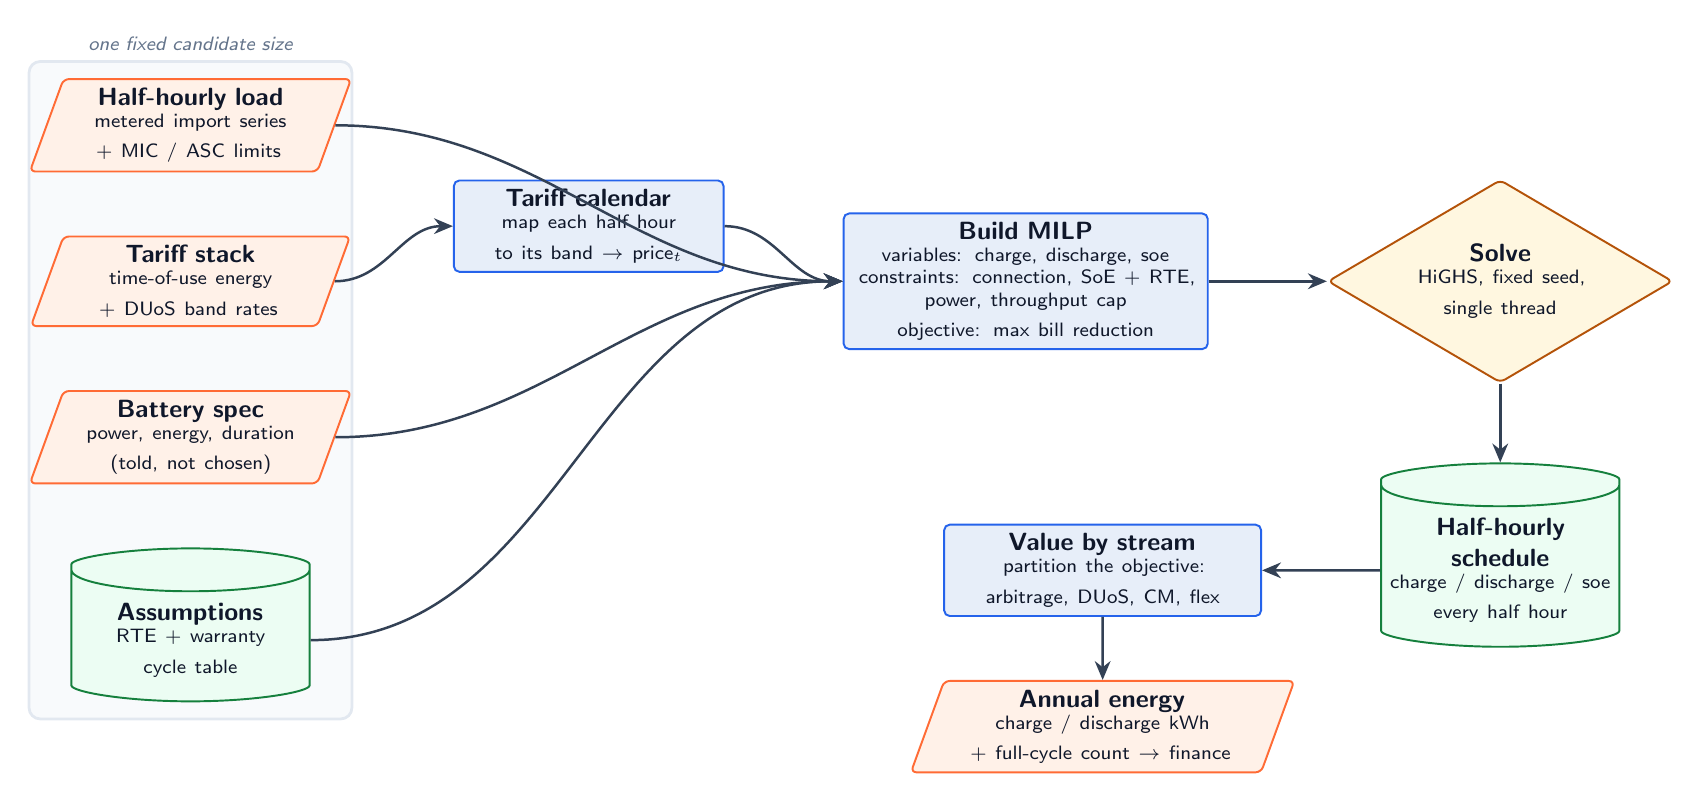
\begin{tikzpicture}[node distance=8mm and 15mm]
  % inputs (left column)
  \node[io] (load) {\textbf{Half-hourly load}\\\scriptsize metered import series\\\scriptsize + MIC / ASC limits};
  \node[io, below=of load] (tariff) {\textbf{Tariff stack}\\\scriptsize time-of-use energy\\\scriptsize + DUoS band rates};
  \node[io, below=of tariff] (spec) {\textbf{Battery spec}\\\scriptsize power, energy, duration\\\scriptsize (told, not chosen)};
  \node[store, below=of spec] (assum) {\textbf{Assumptions}\\\scriptsize RTE + warranty\\\scriptsize cycle table};

  % calendar
  \node[proc, right=of tariff, yshift=7mm] (cal) {\textbf{Tariff calendar}\\\scriptsize map each half hour\\\scriptsize to its band $\rightarrow$ price$_t$};

  % build MILP
  \node[procwide, right=of cal, yshift=-7mm] (build)
     {\textbf{Build MILP}\\\scriptsize variables: charge, discharge, soe\\\scriptsize constraints: connection, SoE + RTE,\\\scriptsize power, throughput cap\\\scriptsize objective: max bill reduction};

  % solve
  \node[decide, right=of build] (solve) {\textbf{Solve}\\\scriptsize HiGHS, fixed seed,\\\scriptsize single thread};

  % schedule
  \node[store, below=of solve, yshift=-2mm] (sched)
     {\textbf{Half-hourly schedule}\\\scriptsize charge / discharge / soe\\\scriptsize every half hour};

  % outputs
  \node[proc, left=of sched, minimum width=40mm, text width=38mm] (value)
     {\textbf{Value by stream}\\\scriptsize partition the objective:\\\scriptsize arbitrage, DUoS, CM, flex};
  \node[io, below=of value, minimum width=40mm, text width=38mm] (energy)
     {\textbf{Annual energy}\\\scriptsize charge / discharge kWh\\\scriptsize + full-cycle count $\rightarrow$ finance};

  % arrows in
  \draw[flow] (load.east) to[out=0,in=180] (build.west);
  \draw[flow] (tariff.east) to[out=0,in=180] (cal.west);
  \draw[flow] (cal.east) to[out=0,in=180] (build.west);
  \draw[flow] (spec.east) to[out=0,in=180] (build.west);
  \draw[flow] (assum.east) to[out=0,in=180] (build.west);
  \draw[flow] (build) -- (solve);
  \draw[flow] (solve) -- (sched);
  \draw[flow] (sched) -- (value);
  \draw[flow] (value) -- (energy);

  % grouping the priced floor inputs
  \begin{scope}[on background layer]
    \node[groupbox, fit=(load)(tariff)(spec)(assum), inner sep=6pt,
          label={[note,anchor=south]north:one fixed candidate size}] {};
  \end{scope}
\end{tikzpicture}}
\caption{One dispatch solve. The site's half-hourly load and connection limits, the tariff stack (priced in time by the calendar), the fixed battery spec, and the assumptions feed the construction of the MILP. The solver returns the half-hourly schedule, which is then valued by stream and reduced to the annual energy volumes finance consumes. The sizing search runs this loop once per candidate size.}
\label{fig:dispatch}
\end{figure}

\section{Valuing the schedule into value-by-stream}

A solved schedule is just numbers until it is attributed to the income streams a lender recognises. The dispatch engine computes the pounds itself, from the solved schedule and the site's tariff; the value stack (Ch.~\ref{ch:valuestack}) is consulted \emph{only} for each stream's gate -- its firmness, whether it is open, and what would unlock it. The attribution partitions the objective with no double-counting.

\begin{table}[H]
\centering
\caption{How the objective is partitioned into value by stream, with no MWh counted twice.}
\label{tab:streams}
\small\sffamily
\begin{tabularx}{\textwidth}{@{}l L@{}}
\toprule
\textbf{Stream} & \textbf{Value attributed} \\
\midrule
Tariff arbitrage & The energy-band part of the bill reduction, net of round-trip losses. A priced floor stream. \\
DUoS red-band avoidance & The DUoS part of the bill reduction, dominated by discharging across the red windows. A priced floor stream. \\
MIC/ASC headroom & \pounds0 by design: its value is already realised through the connection-bounded arbitrage; pricing it separately would double-count the same energy. \\
PPA / bill savings & \pounds0 aggregate: the import-side floor is itemised across arbitrage and DUoS; the PPA rate is set by finance, not here. \\
Capacity Market & Conditional upside: the clearing price times the duration-de-rated capability, held out of the priced floor until deliverability is verified. \\
Local flexibility & Conditional upside: a utilisation rate times the energy delivered in any awarded tender window. \\
Wholesale / BM / ancillary & Gated upside, \pounds0 until a route-to-market partner and export consents exist. \\
\bottomrule
\end{tabularx}
\end{table}

\begin{caution}[Value by stream must sum to the total]
The split above is a partition, not a set of overlapping estimates. Arbitrage and DUoS avoidance together account for the whole priced bill reduction; the headroom and PPA lines are deliberately zero so that the same saved energy is never counted under two headings. Every pound is an assumption-library or tariff number multiplied by a dispatched quantity. A placeholder or needs-review assumption flows through as a loud ``not bankable'' warning attached to its stream, never as a silent figure -- which is why, on the \code{gb\_v0\_1} placeholder library, every result is honestly marked not bankable.
\end{caution}

\section{Annual energy accounting for finance}

Finance needs two annual volumes the dispatch engine alone can produce: the total \textbf{charge} kWh (which carries levies and already includes round-trip losses) and the total \textbf{discharge} kWh (the delivered energy used in pricing to a target return). The schedule sums charge and discharge over the metered horizon and scales them to a full year.

The scaling matters because a metered horizon may be partial. Missing half hours are excluded rather than back-filled -- a load shape is never invented -- so the engine multiplies the horizon totals by an \emph{annual factor} equal to 8760 hours divided by the hours actually covered. From the annual discharge it also derives the equivalent full cycles (annual discharge divided by energy capacity), which is what the warranty check is expressed in. These volumes travel beside the result, not inside the frozen contract; finance reads them through a dedicated hook (Ch.~\ref{ch:engine}, Ch.~\ref{ch:finance}). On thin data, where no schedule solved, both volumes are reported as unavailable rather than zero, so finance stays honestly silent rather than pretending the battery moved no energy.

\section{A representative day}

Alongside the annual totals, the engine can project one real day of the schedule for the application's dispatch chart. It picks the highest-total-discharge full day in the horizon (the earliest such day on a tie), because that is the most legible illustration of the strategy, and copies its half-hourly values verbatim. It is not an average and invents no shape: every point is a genuine solved half hour of one real day. Figure~\ref{fig:day} sketches the pattern such a day typically shows.

\begin{figure}[H]
\centering
\resizebox{\textwidth}{!}{%
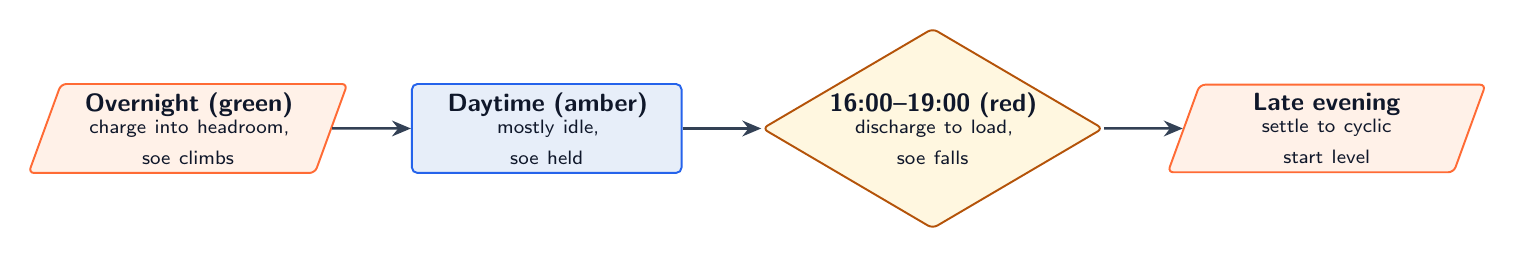
\begin{tikzpicture}[node distance=6mm and 10mm]
  \node[io] (night) {\textbf{Overnight (green)}\\\scriptsize charge into headroom,\\\scriptsize soe climbs};
  \node[proc, right=of night] (day) {\textbf{Daytime (amber)}\\\scriptsize mostly idle,\\\scriptsize soe held};
  \node[decide, right=of day] (peak) {\textbf{16:00--19:00 (red)}\\\scriptsize discharge to load,\\\scriptsize soe falls};
  \node[io, right=of peak] (eve) {\textbf{Late evening}\\\scriptsize settle to cyclic\\\scriptsize start level};
  \draw[flow] (night) -- (day);
  \draw[flow] (day) -- (peak);
  \draw[flow] (peak) -- (eve);
\end{tikzpicture}}
\caption{A representative day of dispatch. The state of energy rises overnight as the battery charges in the cheap green window (within the connection headroom left by the site's load), is held through the day, and falls during the red peak as the battery discharges against the site's load to avoid the most expensive energy and DUoS. The day closes near where it began, honouring the cyclic state-of-energy rule.}
\label{fig:day}
\end{figure}

\section{The real engine and the placeholder seam}

The platform separates \emph{what the optimiser is asked} from \emph{how it answers}, at a fine-grained inner seam: a dispatch solver is anything that takes one fixed system spec plus the site and assumptions and returns a valued, accounted dispatch. Two implementations sit behind that seam.

\begin{description}
  \item[The real MILP solver] is everything described in this chapter: it builds and solves the half-hourly program on an industrial solver (HiGHS, via the linopy modelling layer) and returns genuine site-derived value and genuine annual volumes. It is the default for real runs.
  \item[The placeholder solver] is integration-only scaffolding. It honours the same contract -- it returns the right \emph{shape} of result -- but runs no dispatch: it prices nothing, every stream comes back at zero, and the annual volumes are reported as unavailable, never invented. It exists so the surrounding pipeline could be built and tested before the real solver was written, exactly as the engine seam (Ch.~\ref{ch:engine}) describes at the outer boundary.
\end{description}

The real solver drops in behind the same contract with no downstream change. Both stay honest about being non-bankable until the assumptions behind them are calibrated and confirmed.

\begin{plainnote}[Determinism on the solver]
A linear program could in principle return any of several equally-good schedules, which would break the platform's reproducibility promise. The engine pins this down: the solver runs single-threaded with a fixed random seed and deterministic presolve, the tie-break term makes the optimum unique, and every extracted number is rounded to a fixed precision. The same site, assumptions, and seed therefore produce a byte-for-byte identical schedule every time.
\end{plainnote}

\begin{rebuild}[How to rebuild the dispatch optimiser]
\begin{enumerate}
  \item \textbf{Take one fixed spec as input.} The solver is told the battery's power, energy, and duration; it does not size. Read the half-hourly metered import series and timestamps, the connection limits (MIC, ASC), the tariff stack, the round-trip efficiency, and the warranty cycle table. Never invent a load shape: a missing half-hourly series means \code{insufficient\_data}, no schedule, and no volumes.
  \item \textbf{Build the price signal.} Map each half hour to its tariff band with a time-window calendar (red/amber/green, day/night, or peak/off-peak by period-start clock time), then place the site's own band rates in time. Unrecognised labels or a single flat rate degrade arbitrage to zero with a warning -- never an invented window or price.
  \item \textbf{Define the variables.} For every half hour: charge (kW $\ge 0$, capped at power and at connection headroom), discharge (kW $\ge 0$, capped at power and at site load), and state of energy (kWh, between 0 and energy capacity).
  \item \textbf{Add the constraints.} (a) State-of-energy balance with round-trip efficiency, made cyclic. (b) Charge plus site load never exceeds $\min(\text{MIC}, \text{ASC})$. (c) Discharge never exceeds site load (no export on the floor). (d) Total discharge over the horizon within the warranty throughput budget for the battery's duration (conservative per-duration lookup).
  \item \textbf{Set the objective.} Maximise $\sum_t \text{price}_t (\text{discharge}_t - \text{charge}_t)\,\Delta t$, so round-trip losses are paid at the price faced. Subtract a negligible throughput regulariser to make the optimum unique.
  \item \textbf{Solve deterministically.} Single thread, fixed seed, deterministic presolve, a method that yields a clean vertex solution; round every extracted quantity. Report a non-optimal termination as \code{infeasible} with no schedule.
  \item \textbf{Value and account.} Partition the objective into per-stream value (arbitrage and DUoS as the priced floor; headroom and PPA at zero to avoid double-counting; Capacity Market and local flex as conditional upside; wholesale and friends as gated upside, zero). Sum charge and discharge over the horizon, scale to a year by $8760 \div \text{covered hours}$, and derive equivalent full cycles.
  \item \textbf{Test the invariants:} charge plus load never exceeds the connection in any half hour; equivalent full cycles stay within the warranty for the duration; value by stream sums to the total bill reduction with nothing double-counted; total charge equals total discharge divided by RTE; the same inputs and seed give an identical schedule; and a site with no half-hourly series degrades to no spec without raising.
\end{enumerate}
\end{rebuild}

\begin{keyidea}[The one thing to remember]
The dispatch optimiser writes the battery problem as a mixed-integer linear program -- charge, discharge, and state of energy in every half hour -- and maximises the site's bill reduction subject to hard physics: charging never breaches the grid connection, round-trip losses are paid at the price faced, the warranty cycle cap is never exceeded, and the state of energy stays within bounds and returns to where it started. The solver is pinned to be deterministic; the resulting schedule is valued into a non-overlapping set of streams and reduced to the annual volumes finance underwrites.
\end{keyidea}

\chapter{The sizing optimiser}
\label{ch:sizing}
\modtag{M4}{Sizing optimiser}{Deterministic core}

The previous chapter showed how the platform decides what \emph{one} battery of a given size would earn and cost across a year of half-hourly operation. This chapter answers the question that sits on top of that: \emph{which} battery should the customer actually install? How big should it be?

The sizing optimiser is the layer that chooses the three headline numbers in the system specification: the battery's power (how fast it can charge or discharge, in kilowatts), its duration (how many hours it can sustain that power for), and the energy that the two together imply (power multiplied by duration, in kilowatt-hours). It does this not by guessing or by applying a rule of thumb, but by searching a wide space of candidate sizes (a coarse sweep followed by a seeded refinement, described later in this chapter), running each candidate through the full pricing path, and keeping the size that produces the best return a lender would actually accept.

\begin{plainnote}
A bigger battery earns more, but it also costs more to buy and finance. Somewhere in between is the size that gives the project owner the best return on the money they put in -- but only among the sizes a bank would lend against. The sizing optimiser finds that point by brute force: it prices every candidate and picks the winner. It never invents a system; it only ever chooses from sizes it has fully evaluated.
\end{plainnote}

\pipelinepos{receives a validated \textbf{SiteModel} (Ch.~\ref{ch:contracts}) and the versioned assumptions (Ch.~\ref{ch:assumptions}); hands the chosen specification and the full evaluated grid to the financial model (Ch.~\ref{ch:finance}) and the outputs (Ch.~\ref{ch:outputs}).}

\begin{contract}
\textbf{In:}
\begin{itemize}
  \item A validated \code{SiteModel} (the canonical site: load, connection limits, tariff).
  \item The versioned assumption library (covenant ratio, costs, degradation, durations).
  \item A \emph{search space}: the candidate power and duration values to try.
  \item An injected \emph{dispatch solver} (the half-hourly optimiser of Ch.~\ref{ch:dispatch}), an \emph{objective} (the bankable rule below), and optional \emph{debt terms}.
\end{itemize}
\textbf{Out:} a \code{SizingRun} holding, for every candidate evaluated, its dispatch-and-finance outcome; the chosen optimum (or an honest ``none feasible''); the list of candidates the covenant rejected; and a serialisable \code{SizingGrid} projection that feeds the 3D sizing surface in the outputs.
\end{contract}

\section{Two M4 components: the primitives and the engine that runs them}

It is worth separating two things up front, because the codebase does.

\begin{description}
  \item[The sizing primitives.] A small, self-contained package (\fpath{sizing/}) defines the building blocks: the \emph{search space} (the grid of sizes to try), the \emph{objective} (the rule for which size is best and which are allowed at all), and the \emph{outer loop} that drives a dispatch solver and the financial model over every candidate. These primitives know nothing about how dispatch is actually solved; they are handed a solver and call it.
  \item[The production engine.] A higher layer (\fpath{optimisation/engine.py}) wires the real half-hourly MILP solver into those primitives and exposes the result behind the engine interface that the rest of the platform talks to (the platform/engine seam of Ch.~\ref{ch:engine}). This is where the full evaluated grid is captured and surfaced for plotting.
\end{description}

This split is deliberate. The sizing logic is written once, against an abstract solver, and is ``MILP-ready'': swapping the placeholder solver for the real one changes the numbers but not a single line of the sizing loop.

\begin{keyidea}[One engine, called many times]
The platform does not have a separate ``sizing model'' that approximates returns. It has \emph{one} pricing engine -- dispatch then finance -- and the sizing optimiser simply calls that same engine once for every candidate size, then picks the best answer. Because sizing and the later underwriting re-price both reduce to the identical per-spec primitive, the size the optimiser chooses reprices to exactly the same numbers when underwritten. The specification and the underwriting pack therefore cannot disagree about the battery.
\end{keyidea}

\section{The search space: a grid of power by duration}

The search space is a deterministic, validated grid. It has two axes:

\begin{itemize}
  \item \textbf{Power candidates} (kW). These are always supplied by the caller, never invented inside the sizing code. The right scale for a battery is site-specific -- it is bounded by the site's load, by how much the grid connection can carry, and by physical footprint -- so fabricating an absolute kW figure here would breach the platform's ``no invented site data'' rule. The production engine derives them as fractions of the site's binding capacity (see below).
  \item \textbf{Duration candidates} (hours). These carry a labelled structural default of \code{(1, 2, 4)} hours. Durations are a small, structural set, and the assumption library is already keyed on exactly these values (for warranty cycle caps and Capacity Market de-rating factors). A caller may pass other durations, but values with no library key would have no assumptions to price against. This default injects no money or percentage into any output; it is a structural choice, not a hidden financial constant.
\end{itemize}

Each axis is validated on construction: every value must be a strictly positive number (a zero-kW or zero-hour battery is not a candidate, and negatives are rejected outright), and each axis is de-duplicated and sorted ascending. The grid itself is the Cartesian product of the two axes, enumerated in a fixed \code{(power, duration)} order so that two runs on the same inputs produce candidates in the same sequence.

\begin{table}[H]
\centering
\caption{The search space and each candidate. Energy is always derived, never an independent input.}
\label{tab:searchspace}
\small\sffamily
\begin{tabularx}{\textwidth}{@{}l l L@{}}
\toprule
\textbf{Quantity} & \textbf{Unit} & \textbf{Rule} \\
\midrule
Power axis & kW & Caller-supplied; strictly positive; de-duplicated; sorted ascending. \\
Duration axis & h & Default \code{(1, 2, 4)}; caller may override; same validation. \\
Candidate & -- & One \code{(power, duration)} pair from the Cartesian product. \\
Energy & kWh & \emph{Derived}: \code{energy\_kwh = power\_kw $\times$ duration\_hours}, rounded to 6 d.p. \\
Enumeration order & -- & By the \code{(power, duration)} tuple, ascending -- deterministic. \\
\bottomrule
\end{tabularx}
\end{table}

\begin{caution}[Energy is derived, and order is by power-then-duration]
A candidate stores only power and duration; its energy is computed from them on demand, so the three numbers can never drift apart. Enumeration is ordered by the \code{(power, duration)} pair, \emph{not} by derived energy: a 100\,kW $\times$ 4\,h system and a 200\,kW $\times$ 2\,h system both hold 400\,kWh, so ordering by energy would be ambiguous for such ties. An empty axis yields no candidates, and the loop treats that as ``nothing to evaluate'' rather than an error.
\end{caution}

\subsection{How the production engine searches: the two-stage continuous search}

When the real engine sizes a site it does not ask a human for power candidates. Its default search is the labelled three-by-three grid; the two-stage continuous search described here is built and verified but \textbf{opt-in}, because on the shipped assumption releases capital cost is keyed per megawatt only -- added duration earns revenue at zero marginal capital cost, so any wide-duration search pins its recommendation to the band edge. That is a placeholder artifact, not an optimum, and the engine refuses to present it as one until the capital-cost shape gains an energy component (the C025 gate). Either search scales to the site's \emph{binding capacity}: the observed peak import if the site has metered load, otherwise the contracted connection limit (the maximum import capacity, or MIC). If the site has neither, there is no honest basis to scale from, and the engine returns a no-specification result rather than guessing.

The search then runs in three stages, all deterministic:

\begin{enumerate}
  \item \textbf{Coarse sweep.} Ten labelled structural power fractions spanning 5 to 150 percent of the binding capacity are paired with eight durations from half an hour to eight hours. Every cell is priced through the full pricing path, but against a \emph{typical-period proxy}: one representative metered day per calendar stratum (each month, split weekday against weekend), chosen as the day closest to its peers (the medoid) and weighted by how many complete days it stands for. Only complete, gap-free days qualify; nothing is filled in or invented, and each proxy result is labelled as such.
  \item \textbf{Seeded refinement.} A small evolutionary loop (differential evolution, driven by a fixed seed, with every evaluation memoised) explores the same continuous box, starting from the best coarse cells, for a budget of roughly two hundred evaluations. It is free to land between the coarse cells: durations such as 2.7 hours are real candidates. Duration-keyed assumption tables keep the conservative-flooring lookup (the largest tabulated duration at or below the candidate's); interpolating between tabulated points is deferred until sourced warranty and de-rating content lands. One caution travels with that choice: the warranty cycle table \emph{decreases} with duration, so flooring an off-key duration inherits the shorter duration's higher cap -- a known generosity, flagged for the interpolation-policy decision rather than silently accepted.
  \item \textbf{Confirmation and polish.} A diverse set of top-ranked candidates (up to ten; near-clones are skipped so the set covers the optimum region, not one point) is re-solved on the \emph{full} metered series, followed by a bounded compass polish around the best confirmed candidate (a handful of exact solves, deterministic step schedule). The \emph{best} confirmed candidate that clears the covenant wins -- never merely the first to pass -- and only confirmed evaluations can be selected or reported.
\end{enumerate}

\begin{caution}[Proxy numbers guide, confirmed numbers report]
The typical-period proxy exists to make a few hundred candidate evaluations affordable; it is search guidance, not an answer. Every proxy evaluation is labelled (a \code{proxy} flag and a provenance warning on the result), the chosen size is always re-solved on the full metered year before anything downstream sees it, and the engine's indicative fallback never picks a proxy evaluation. No reported number ever comes from an approximation.
\end{caution}

Every candidate evaluated in any stage is kept and persisted (stage-labelled) as the sizing cloud, so the plotted surface is a genuinely continuous picture of the trade-off space rather than nine points. The legacy three-by-three grid is the engine default (pending the C025 gate above) and the honest fallback when no metered series is available, where each candidate degrades to an insufficient-data result exactly as before.

\section{The bankable objective: maximise return, subject to the covenant}

The rule for ``best'' is the heart of the module. Stated plainly:

\begin{quote}\sffamily
Search power, energy and duration to maximise the \emph{levered} (equity) return, subject to the hard constraint that the conservative P90 debt service cover ratio stays at or above its covenant.
\end{quote}

Two terms need unpacking for a non-specialist reader.

\begin{description}
  \item[Levered (equity) return.] The return on the cash the project's owners actually invest, after the loan is serviced. Because debt is cheaper than equity, borrowing amplifies (``levers'') the equity return. This is the finance model's equity internal rate of return (IRR) on the central P50 case, and it is the number sizing tries to make as large as possible.
  \item[P90 DSCR covenant.] DSCR is the debt service cover ratio: the cash a project generates in a year divided by the loan repayment due that year. A DSCR of 1.0 means the cash exactly covers the repayment; lenders demand a comfortable cushion above 1.0. The \emph{P90} DSCR is that ratio computed on a deliberately pessimistic (one-in-ten bad) cashflow. The \emph{covenant} is the minimum P90 DSCR the lender will accept. (See Ch.~\ref{ch:finance} and Appendix~\ref{app:glossary}.)
\end{description}

The crucial design choice is that the covenant is \emph{embedded inside the objective as a feasibility gate}, not bolted on as a check afterwards. A candidate the covenant would reject can never be selected, because the optimiser only ever ranks candidates that have already passed the gate.

\subsection{The feasibility gate, exactly}

A candidate is \emph{feasible} only if all of the following hold. If any fails, the candidate is not eligible to win, no matter how high its return:

\begin{table}[H]
\centering
\caption{The feasibility gate. A missing input never counts as a pass.}
\label{tab:gate}
\small\sffamily
\begin{tabularx}{\textwidth}{@{}l L@{}}
\toprule
\textbf{Condition} & \textbf{Why, and what a missing value means} \\
\midrule
Covenant known & The minimum P90 DSCR must be read from the assumption library. If it is unknown, \emph{no} candidate can be proven feasible. \\
P90 DSCR available & The candidate's P90 DSCR must have been computed. It is only available when real debt terms are injected, because the library carries no debt structure in v1. Unavailable means not feasible -- never an assumed pass. \\
P90 DSCR $\ge$ covenant & The conservative cover ratio must meet or beat the covenant. \\
Not known non-deliverable & The spec must not have an explicit ``cannot be delivered to end of life'' verdict (see below). \\
\bottomrule
\end{tabularx}
\end{table}

\begin{caution}[A missing number is never a silent pass]
The gate is built so that absence of evidence is treated as failure, not success. No covenant, no DSCR, or an explicit non-deliverable verdict all make a candidate infeasible. A \code{None} value is never compared as if it were a number. This is what lets the platform run honestly on placeholder data: when the inputs to prove bankability are absent, nothing is declared bankable.
\end{caution}

\subsection{Ranking the feasible candidates}

Among the candidates that pass the gate, the optimiser picks the maximum under a deterministic ranking key. The key prefers, in strict order: first a candidate that has a levered return at all, then the higher levered return; then (only as a labelled fallback when no debt is injected and there is no levered split) a candidate that has an unlevered project IRR, then the higher project IRR; then, as a tie-break, the \emph{smaller} system -- smaller power first, then smaller duration. Unavailable metrics sort last via an availability flag, so a missing number is never treated as a value. The smaller-system tie-break means that when two sizes earn the same return, the platform recommends the cheaper, less over-built one.

\begin{keyidea}[The levered return is the primary metric, and it is honest about itself]
The objective ranks first on the equity (levered) return, which exists only when real debt terms are supplied. Without debt there is no levered split, so the optimiser falls back to ranking on the unlevered project return and explicitly flags that a ranking on the fallback is \emph{not yet a bankable optimisation}. It never fabricates a levered figure to fill the gap.
\end{keyidea}

\section{Sizing day-one for end-of-life capability}

A battery degrades over its life: it holds less energy and earns less each year. The platform sizes the system \emph{day one for its end-of-life duty}, with no augmentation (no mid-life top-up of cells). The consequence is subtle and important: the year that decides whether the project clears its covenant -- the \emph{binding} year -- may be late in the asset's life, when degradation has eaten into the cashflow and the P90 DSCR is at its weakest.

This is handled cleanly by the division of labour. Degradation already flows through the financial model: revenue fades over the years, so the late-life P90 cashflow is lower, so the late-life P90 DSCR is lower. The sizing objective therefore does \emph{not} re-model degradation. The feasibility gate consumes the P90 DSCR that finance has already computed across the whole horizon, and the conservative (minimum across years) value is the one tested against the covenant. The only extra thing the gate does is reject a spec carrying an \emph{explicit} ``not deliverable to its final contract year'' verdict.

\begin{caution}[Unassessed deliverability is a data-ask, not a pass]
In the current placeholder world there is no signal that verifies late-life deliverability, so that verdict is recorded as \emph{unassessed} rather than fabricated to a pass. An unassessed verdict does not block a candidate (it is logged as a piece of data that would improve the quote); only an explicit \emph{false} verdict rejects it. A true verdict is only ever set by a real engine that has checked it. This follows the platform's honest-degradation principle: never invent a capability you have not verified.
\end{caution}

\section{The outer loop, step by step}

Figure~\ref{fig:sizingloop} shows the whole loop. For each candidate in the enumerated grid the optimiser runs the same three steps: solve the dispatch, evaluate the finance, and test the covenant. Feasible candidates are kept; the best of them is selected; and the chosen specification plus the full grid are returned.

\begin{figure}[H]
\centering
\resizebox{\textwidth}{!}{%
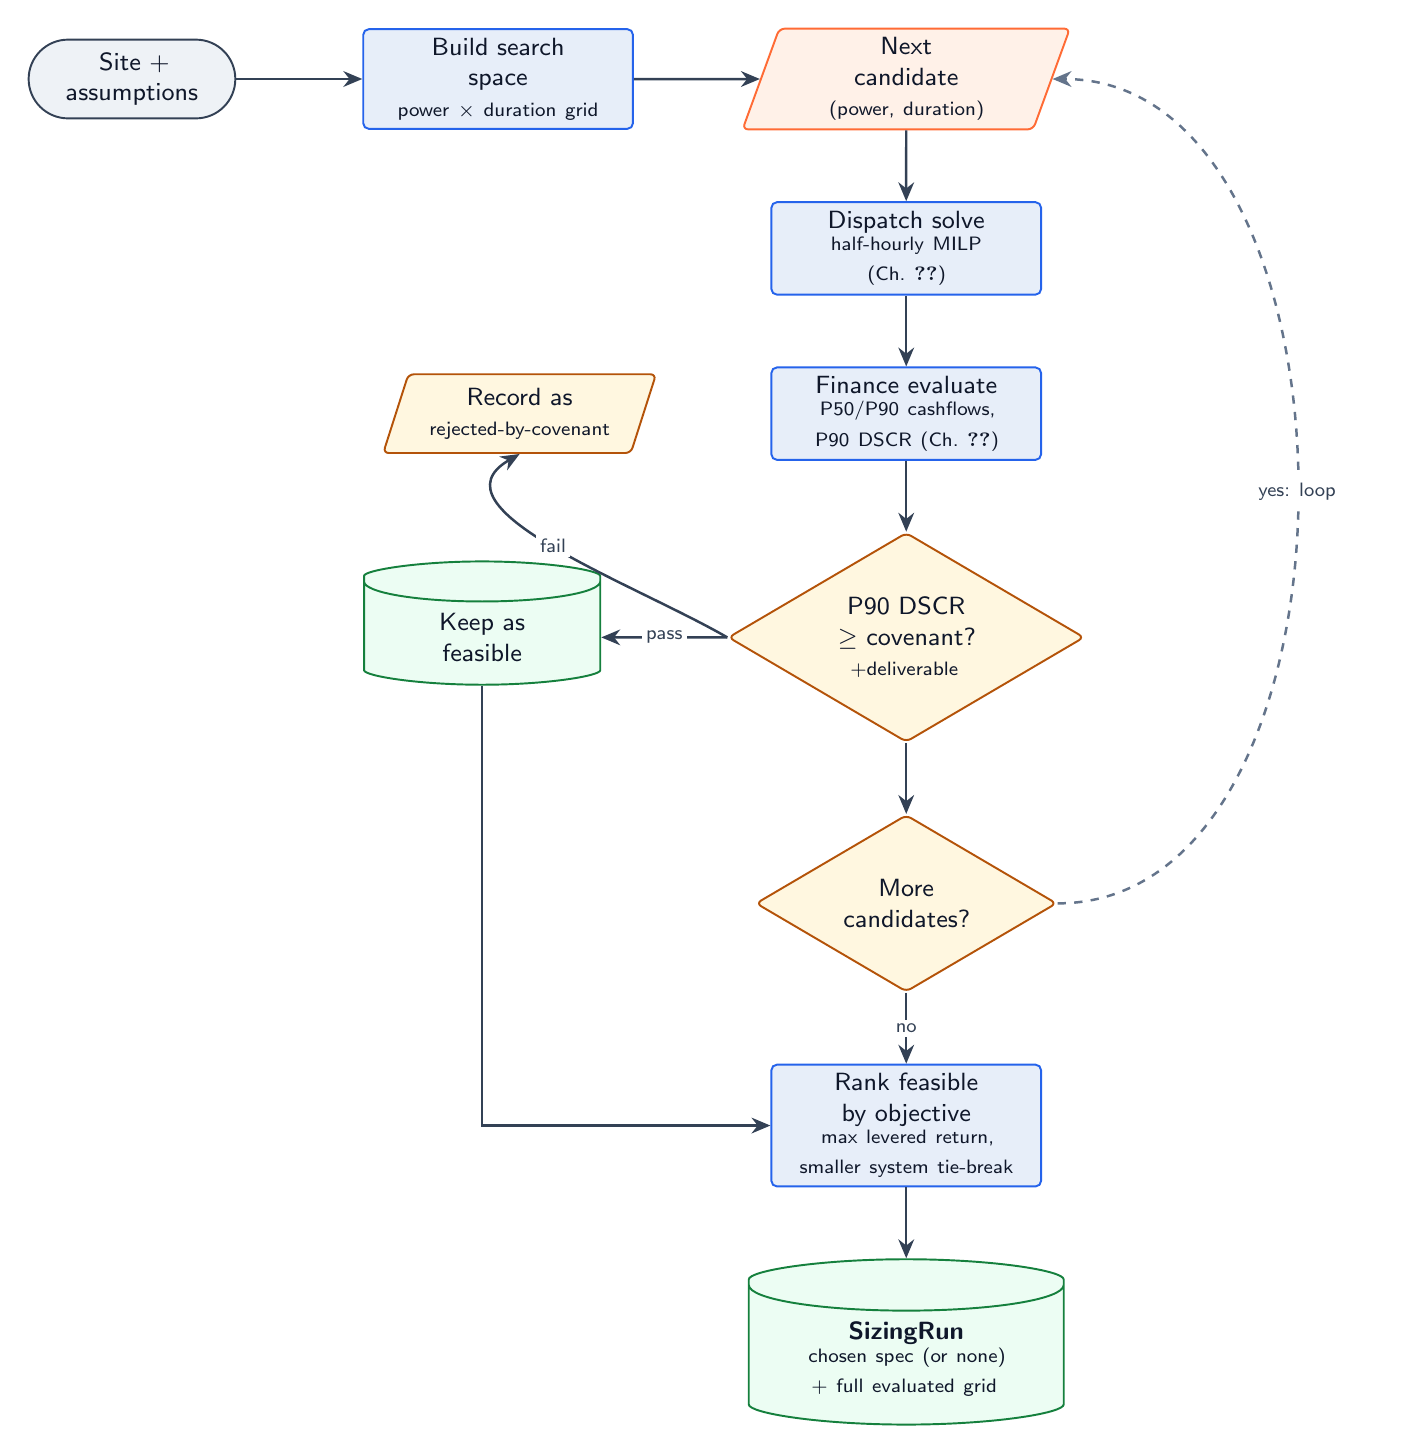
\begin{tikzpicture}[node distance=9mm and 16mm]
  \node[term] (start) {Site +\\assumptions};
  \node[proc, right=of start] (grid) {Build search\\space\\\scriptsize power $\times$ duration grid};
  \node[io, right=of grid] (cand) {Next\\candidate\\\scriptsize (power, duration)};

  % the per-candidate pipeline
  \node[proc, below=of cand] (dispatch) {Dispatch solve\\\scriptsize half-hourly MILP\\\scriptsize (Ch.~\ref{ch:dispatch})};
  \node[proc, below=of dispatch] (finance) {Finance evaluate\\\scriptsize P50/P90 cashflows,\\\scriptsize P90 DSCR (Ch.~\ref{ch:finance})};
  \node[decide, below=of finance] (gate) {P90 DSCR\\$\ge$ covenant?\\\scriptsize +deliverable};

  \node[store, left=of gate, text width=26mm] (keep) {Keep as\\feasible};
  \node[io, left=of finance, text width=26mm, fill=nodeDecision, draw=nodeDecisionBd] (reject)
       {Record as\\\scriptsize rejected-by-covenant};

  % after the loop
  \node[decide, below=of gate] (more) {More\\candidates?};
  \node[proc, below=of more] (rank) {Rank feasible\\by objective\\\scriptsize max levered return,\\\scriptsize smaller system tie-break};
  \node[store, below=of rank, text width=34mm, minimum width=40mm] (out)
       {\textbf{SizingRun}\\\scriptsize chosen spec (or none)\\\scriptsize + full evaluated grid};

  % flow
  \draw[flow] (start) -- (grid);
  \draw[flow] (grid) -- (cand);
  \draw[flow] (cand) -- (dispatch);
  \draw[flow] (dispatch) -- (finance);
  \draw[flow] (finance) -- (gate);
  \draw[flow] (gate) -- node[flowlabel]{pass} (keep);
  \draw[flow] (gate.west) to[out=150,in=-150] node[flowlabel]{fail} (reject.south);
  \draw[flow] (gate) -- (more);
  \draw[flowback] (more.east) to[out=0,in=0] node[flowlabel]{yes: loop} (cand.east);
  \draw[flow] (more) -- node[flowlabel]{no} (rank);
  \draw[flow] (keep) |- (rank.west);
  \draw[flow] (rank) -- (out);
\end{tikzpicture}}
\caption{The sizing outer loop. The search space is enumerated; each candidate is dispatch-solved, finance-evaluated, and tested against the P90 DSCR covenant gate; feasible candidates are kept and the loop repeats; the best feasible candidate is selected; the chosen specification and the full evaluated grid are returned. The dashed arrow is the loop over candidates; the amber diamond is the covenant gate.}
\label{fig:sizingloop}
\end{figure}

\subsection{What happens to one candidate}

The per-candidate work is a single shared primitive -- the same one the standalone underwriting re-price uses -- so that sizing and underwriting can never drift. For one fixed candidate it:

\begin{enumerate}
  \item Builds a dispatch problem (the site, the assumptions, this candidate's power, energy and duration, the requested income streams and their constraints) and calls the injected dispatch solver.
  \item Maps the solver's result onto the frozen \code{OptimisationResult} contract, carrying the implementation level and bankable status straight through (the placeholder is always BASELINE / not-bankable, which the schema enforces).
  \item Runs the deterministic financial model on that result, threading through the candidate's annual charge and discharge volumes so finance can compute charging levies and the price-to-target.
  \item Reads off the metrics the objective needs: the minimum P90 DSCR (if available), the covenant and whether the candidate passes it, the levered (equity) return, and the unlevered project IRR.
\end{enumerate}

\begin{caution}[An unpriceable candidate is recorded, not dropped]
If the financial model cannot build a cashflow for a candidate (for example a dispatch that produced no positive sizing), that candidate is recorded with \code{priceable = false} and carries on; it is never selected and never raises an error. Honest accounting keeps every candidate visible in the grid, including the ones that could not be priced.
\end{caution}

\subsection{Selection and the bankable flag}

After the loop, the feasible candidates are ranked and the maximum is selected. The run's overall \code{bankable} flag is set to true \emph{only} if the selected candidate is itself bankable \emph{and} its primary metric (the levered return) was actually computed. On the placeholder assumption set this can never be true, so every sizing run is honestly not bankable. The run also separately records the candidates the covenant \emph{explicitly} rejected (those whose DSCR was available but fell short), kept distinct from candidates whose DSCR was simply unavailable.

\begin{keyidea}[At least one grid point is rejected, so the gate demonstrably fires]
When real debt terms make the P90 DSCR computable, the grid is constructed so that at least one candidate fails the covenant and lands on the rejected-by-covenant list. This is not incidental: it is how the platform \emph{proves} the bankable gate is live rather than vacuous. A run where nothing was ever rejected could not demonstrate that the constraint is doing any work. The rejected list is the evidence that a sub-covenant size was offered up and turned away.
\end{keyidea}

\section{The full evaluated grid and the sizing surface}

The frozen \code{OptimisationResult} carries only the \emph{chosen} candidate's specification. But the platform also needs the full picture -- every candidate it tried and how each scored -- so the proposal can show the customer \emph{why} this size, on an interactive 3D ``sizing surface''. That surface plots power against duration against levered return, highlights the region that meets the P90 DSCR covenant, and marks the chosen optimum.

The sizing run therefore projects itself into a separate, serialisable \code{SizingGrid} record. This is an \emph{additive seam}: it copies each candidate's plottable scalars straight off its evaluation, inventing nothing, and is persisted alongside the quote without adding any field to the frozen result. The production engine captures the whole run on every solve -- even when no candidate produced a spec, so the surface can still show an honestly infeasible grid -- and exposes it for the quote pipeline to persist.

\begin{table}[H]
\centering
\caption{What each point of the persisted sizing grid carries. Every field is copied from the evaluation; an unavailable metric stays \code{None}, never coerced to a number.}
\label{tab:gridpoint}
\small\sffamily
\begin{tabularx}{\textwidth}{@{}l l L@{}}
\toprule
\textbf{Field} & \textbf{Unit} & \textbf{Meaning} \\
\midrule
power\_kw & kW & The candidate's power. \\
duration\_hours & h & The candidate's duration. \\
energy\_kwh & kWh & Derived: power $\times$ duration. \\
levered\_return\_pct & \% & Equity IRR (P50 basis); \code{None} without injected debt -- the surface's height axis. \\
project\_irr\_pct & \% & Unlevered project IRR (the labelled fallback). \\
min\_p90\_dscr & ratio & Conservative cover ratio; \code{None} when no debt structure. \\
passes\_covenant & true/false/none & Feasibility flag: \code{None} when DSCR is unavailable, never forced to false. \\
priceable & bool & Whether finance could build a cashflow at all. \\
bankable & bool & Whether this candidate cleared the bankable bar. \\
solver\_status & enum & The dispatch solver's status for this candidate. \\
end\_of\_life\_deliverable & true/false/none & Late-life capability verdict (\code{None} = unassessed data-ask). \\
\bottomrule
\end{tabularx}
\end{table}

The grid-level record wraps these points with the search-space size, the covenant the feasibility flags were measured against, the overall bankable flag, the human-readable selection reason, and the chosen optimum (or \code{None} when no candidate met the covenant -- honest, not an error).

\section{Why sizing and underwriting cannot disagree}

The platform makes a strong promise: the size in the customer proposal is the same size the lender underwrote, priced to the same numbers. The sizing module is where that promise is made structural. Sizing \emph{searches} specifications; underwriting \emph{prices} the chosen one. Both reduce to the identical per-spec primitive -- same dispatch solver, same value stack, same finance model. The underwriting re-price is deliberately handed only the raw inputs (site, assumptions, the chosen spec), not the sizer's pre-built result, and it reconstructs the dispatch-and-finance path independently. Because both paths run the same deterministic primitive on the same canonical inputs, the chosen spec reprices to byte-identical numbers. A timestamp-free \emph{financial fingerprint} (the load-bearing finance numbers, with the wall-clock metadata excluded) is compared between the two to prove it. The optimiser therefore cannot select a spec that underwriting would reject.

\begin{rebuild}
To re-implement the sizing optimiser from scratch:
\begin{enumerate}
  \item \textbf{Search space.} Define an immutable candidate as \code{(power\_kw, duration\_hours)} with energy \emph{derived} as their product (never stored independently). Validate both axes as strictly positive numbers; de-duplicate and sort each ascending. The grid is the Cartesian product, enumerated in \code{(power, duration)} order. Give duration a labelled structural default of \code{(1, 2, 4)} hours; require the caller to supply power candidates (or, in the production engine, scale them as fractions \code{(0.25, 0.5, 1.0)} of the site's observed peak, falling back to its connection limit).
  \item \textbf{Objective.} Hold the covenant ratio. Expose a \emph{feasibility} test that returns true only if: the covenant is known, the P90 DSCR is available, the P90 DSCR meets the covenant, and the deliverability verdict is not explicitly false. Treat every missing value as failure. Expose a deterministic \emph{rank key} that maximises the levered return first, falls back to the project IRR, and tie-breaks toward the smaller system; sort unavailable metrics last via an availability flag so \code{None} is never compared as a number.
  \item \textbf{Per-spec primitive.} Write one function that, for a fixed spec, builds a dispatch problem, calls an \emph{injected} solver, maps the result onto the frozen result contract, runs the financial model (threading dispatch volumes through), and returns the metrics the objective reads. Catch an unpriceable result and record it (\code{priceable = false}); never raise.
  \item \textbf{Outer loop.} Enumerate the grid; evaluate each candidate via the primitive; collect the covenant-rejected ones separately. Filter to the feasible set; take the maximum under the rank key. Set the run's \code{bankable} flag true only when the selected candidate is bankable \emph{and} its levered metric exists. Return all evaluations, the selection, the rejected list, and the reason.
  \item \textbf{Grid projection.} Project the run into a serialisable grid of plottable scalars (copy, no arithmetic), preserving enumeration order; carry the covenant and the chosen optimum (or none). Persist this additively, without adding fields to the frozen result.
  \item \textbf{Production engine.} Compose the loop with the real MILP solver behind the engine interface; degrade to a no-spec result when there is no sizing basis or no dispatch; expose the captured run and dispatch volumes as duck-typed hooks for the quote pipeline.
\end{enumerate}
\textbf{Invariants to test:} energy always equals power $\times$ duration; enumeration order is deterministic and stable across runs; a missing covenant or DSCR yields no feasible candidate; with real debt at least one candidate is rejected by the covenant; the chosen spec's underwriting re-price has an identical financial fingerprint; \code{bankable} is never true on the placeholder solver.
\end{rebuild}

\chapter{The scenario engine}
\label{ch:scenarios}
\modtag{M6}{Scenario engine}{Deterministic core}

A lender does not want a single number for what a battery will earn. The future is uncertain: power prices might be soft or strong, a grant might land or lapse, the project might switch on a year later than planned. The lender wants to know what the project earns in a normal year and what it earns in a bad year, so it can size a loan against the bad year and still be paid back. The scenario engine is the part of the platform that turns ``the future is uncertain'' into exactly those two numbers, in a way that can be audited line by line.

It does this without any guesswork dressed up as precision. Instead of simulating thousands of random futures, the engine evaluates a small, named handful of cases -- a Low one, a Central one, and a High one -- each carrying a stated probability, and reads two figures off the resulting spread: a central estimate (the ``P50'') and a conservative one (the ``P90''). Those two figures are what the financial model turns into cashflows and what the lender underwrites.

\begin{plainnote}
\textbf{P50 and P90 in plain words.} Imagine ranking every plausible outcome from worst to best. The \emph{P50} is the one in the middle: a coin-flip says the real outcome is higher or lower, so it is the honest ``expected'' figure. The \emph{P90} is a pessimistic one: the outcome should be at least this good about nine times out of ten. Lenders lend against the P90 because they are paid back out of the bad years, not the good ones. The scenario engine's job is to produce a defensible P50 and P90 rather than a single, falsely confident point estimate.
\end{plainnote}

\pipelinepos{receives a base case (the P50 and P90 cashflows of one priced battery, Ch.~\ref{ch:finance}), the versioned scenario weights and price bands (Ch.~\ref{ch:assumptions}), and any pinned external price forecast; hands a weighted P50/P90 distribution to the financial model (Ch.~\ref{ch:finance}) and a per-case price series to the dispatch optimiser (Ch.~\ref{ch:dispatch}).}

\begin{contract}
\textbf{In:}
\begin{itemize}
  \item A \emph{base case} exposing two cashflow series, \code{p50\_cashflows} and \code{p90\_cashflows} (one figure per modelled year, year~0 being the capex outflow). Any object with these two lists satisfies the engine; in practice it is a priced \code{FinancialCase}.
  \item A \emph{scenario set}: the Low / Central / High cases to evaluate together, each with a probability weight, a price multiplier, a cost multiplier, and a time-to-energisation delay. Weights are read from the versioned assumption library (Ch.~\ref{ch:assumptions}); price and cost bands are explicit, sourced input.
  \item Optionally, a hash-pinned \code{ForecastReference} to an external price curve (for example a Modo Energy wholesale forecast), carried as provenance only.
\end{itemize}
\textbf{Out:} a \code{ScenarioRunResult} holding one evaluated \code{ScenarioResult} per case and a \code{WeightedSummary} -- the probability-weighted P50 and P90 cashflow series and their undiscounted totals -- stamped with the assumption version, a machine-readable bankable status, and every warning the run accumulated. The engine never produces a valuation: no discounting, no internal rate of return, no debt cover. Those belong to the financial model.
\end{contract}

\section{Discrete cases, not a cloud of draws}

The engine's central design choice is to be \emph{honestly coarse}. Rather than draw a continuous probability distribution over the future and sample it, it evaluates a few named cases and reports the spread between them. Each case is one \emph{scenario}, and the cases evaluated together are a \emph{scenario set}.

A scenario is a small, self-contained description of one possible future, built from sourced parameters and nothing invented:

\begin{table}[H]
\centering
\caption{The fields of one scenario. Every value is either explicit, sourced input or read from the assumption library; none is fabricated inside the engine.}
\label{tab:scenariofields}
\small\sffamily
\begin{tabularx}{\textwidth}{@{}l l L@{}}
\toprule
\textbf{Field} & \textbf{Type} & \textbf{Meaning and rule} \\
\midrule
Name & label & One of \code{low}, \code{central}, \code{high}, or \code{custom}. \\
Probability weight & 0--1 & How likely this case is. Across a set the weights should sum to 1.0. \\
Price multiplier & $>0$ & Scales the operating-year (revenue-driven) cashflows. \code{1.0} means no change. \\
Cost multiplier & $>0$ & Scales the year-0 capex outflow. \code{1.0} means no change. \\
COD delay (months) & $\geq 0$ & Months the commercial operation date slips. Affects \emph{timing} only. \\
Policy branch & label & A descriptive policy-axis tag. In v1 it carries no numeric effect by itself. \\
Forecast reference & optional & A hash-pinned pointer to an external price curve, if one backs this case. \\
\bottomrule
\end{tabularx}
\end{table}

Central is special: it is the base case itself, with every multiplier set to \code{1.0} and no delay. So evaluating the Central scenario reproduces the input cashflows exactly. Low and High then express the downside and upside as multipliers relative to that anchor.

\begin{keyidea}[Honest coarseness beats false precision]
A lender reviews a handful of named, defensible cases far more readily than a fan chart of thousands of random draws. More importantly, while the platform runs on placeholder assumptions, simulating thousands of futures over un-calibrated inputs would manufacture confidence the inputs cannot support. A small set of weighted cases keeps the coarseness visible and the reasoning legible. That is a deliberate choice, not a missing feature.
\end{keyidea}

\section{How a case is applied to the base cashflows}

Given a scenario, the engine transforms the base case's two cashflow series (P50 and P90 alike) in a fixed order. The transformation is deliberately simple and first-order, because a coarse-but-honest adjustment is preferable to a precise-looking one the inputs cannot justify.

\begin{enumerate}
  \item \textbf{Scale by the multipliers.} The year-0 figure (the capex outflow) is multiplied by the \emph{cost} multiplier; every later year (the operating cashflows) is multiplied by the \emph{price} multiplier. This is a first-order revenue and cost sensitivity applied to the net series, not a split into income lines the engine cannot justify from a net figure.
  \item \textbf{Shift for the energisation delay.} If the commercial operation date (COD, the day the battery starts earning) slips by a whole number of years, the operating cashflows are pushed that many years later. The capex stays at year~0. Revenue that would fall beyond the modelled horizon is dropped, never created: a delay defers income, it does not invent it.
  \item \textbf{Total the result.} The engine sums each adjusted series into an undiscounted P50 total and P90 total for that case. These are coarse running totals for comparison, not present values.
\end{enumerate}

Several edge cases are handled explicitly rather than silently:

\begin{table}[H]
\centering
\caption{Edge cases in applying a scenario, and how the engine responds. The pattern is always to warn rather than to fake a number or to fail.}
\label{tab:scenarioedge}
\small\sffamily
\begin{tabularx}{\textwidth}{@{}L L@{}}
\toprule
\textbf{Situation} & \textbf{Response} \\
\midrule
Year-0 cashflow is non-negative (no capex outflow where one is expected) & Apply the cost multiplier anyway, and warn to confirm the cashflow sign convention. \\
A delay that is \emph{not} a whole number of years (a sub-annual slip) & Leave timing unchanged and warn: v1 models COD at annual granularity only, so a month-level shift would be false precision. \\
The base case has only a year-0 figure and no operating years & The price multiplier has no effect; warn so the caller is not misled. \\
Any cashflow is infinite or not-a-number & Warn loudly: the scenario totals will also be non-finite, and the base case must be fixed first. \\
\bottomrule
\end{tabularx}
\end{table}

\begin{caution}[The policy branch is a label, never a hidden number]
A scenario carries a \emph{policy branch} tag so a case can be described as, say, a particular subsidy regime. In v1 that label changes no figure on its own. Any policy effect must be carried by the explicit price and cost multipliers or the delay, all of which must themselves be sourced. A non-default branch is automatically flagged ``descriptive only'' so a tag can never smuggle uncalibrated precision into the numbers.
\end{caution}

\section{Weights, and reading P50 and P90 off the set}

Once each case has been evaluated, the engine combines them into the two figures the lender needs. The combining step is a probability-weighted average across the cases, performed element by element across the years.

The weights come from the assumption library, under a single versioned entry (\code{scenario\_weights.\allowbreak central\_low\_high}), so the relative likelihood of Low, Central, and High is content that can be versioned and audited, never a constant buried in code (Ch.~\ref{ch:assumptions}). Discrete weights such as 0.25 / 0.50 / 0.25 are meant to sum to 1.0. The engine enforces this honestly rather than silently:

\begin{itemize}
  \item If the weights already sum to 1.0 (within a tiny floating-point tolerance) they are used unchanged.
  \item If they do not, they are \emph{normalised} -- divided by their total so they sum to 1.0 -- and a warning records that this happened, so a mis-weighted set is never used silently.
  \item If the weights sum to zero or less (which cannot be normalised), the engine falls back to equal weights and warns, rather than dividing by zero or inventing a distribution.
\end{itemize}

The weighted P50 series is then the sum, year by year, of each case's P50 series multiplied by its normalised weight; the weighted P90 series is formed the same way from the cases' P90 series. Series of different lengths are zero-padded to the longest horizon before summing, so a delayed case with a shorter effective operating life still combines correctly.

\begin{plainnote}
\textbf{Why two series, not one.} The base case already carries its own P50 and P90 cashflows: the central and conservative views of \emph{one} battery's economics. The scenario engine layers the Low / Central / High price-and-policy spread on \emph{top} of that, applying each case's multipliers to both series. The result is a weighted P50 (the headline expected cashflow) and a weighted P90 (the conservative cashflow the loan is sized against). The two ideas -- the conservatism already inside a single case, and the spread across cases -- stack rather than compete.
\end{plainnote}

Figure~\ref{fig:scenflow} shows the whole flow: versioned cases and weights produce a weighted distribution, from which P50 and P90 are read and handed to the value stack and the financial model.

\begin{figure}[H]
\centering
\resizebox{\textwidth}{!}{%
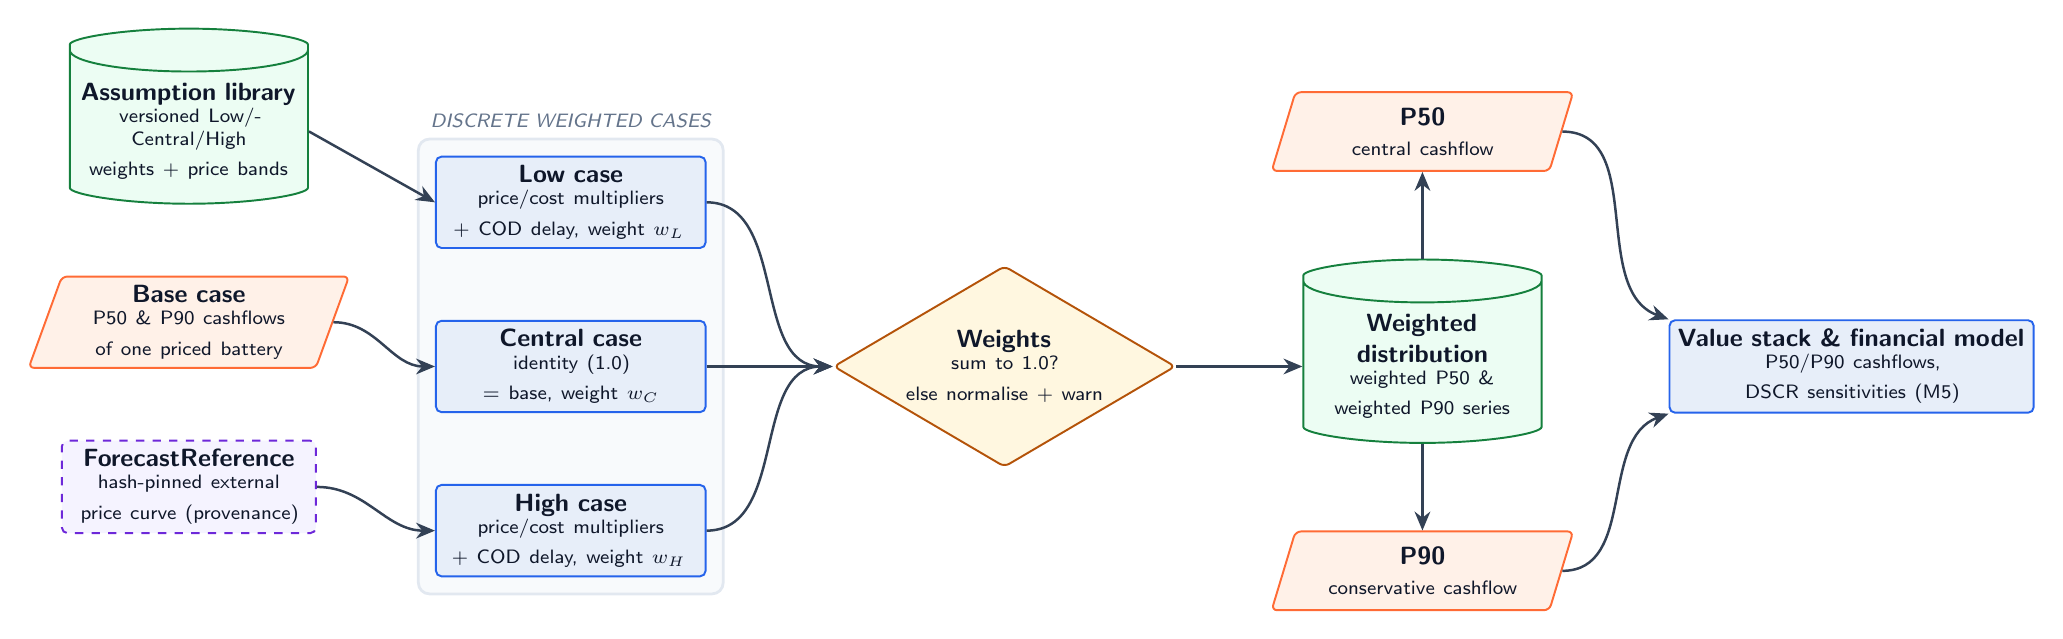
\begin{tikzpicture}[node distance=9mm and 16mm]
  % inputs on the left
  \node[store] (assum) {\textbf{Assumption library}\\\scriptsize versioned Low/Central/High\\\scriptsize weights + price bands};
  \node[io, below=of assum] (base) {\textbf{Base case}\\\scriptsize P50 \& P90 cashflows\\\scriptsize of one priced battery};
  \node[ext, below=of base] (forecast) {\textbf{ForecastReference}\\\scriptsize hash-pinned external\\\scriptsize price curve (provenance)};

  % the three cases
  \node[proc, right=of assum, yshift=-9mm] (low) {\textbf{Low case}\\\scriptsize price/cost multipliers\\\scriptsize + COD delay, weight $w_L$};
  \node[proc, below=of low] (central) {\textbf{Central case}\\\scriptsize identity (1.0)\\\scriptsize $=$ base, weight $w_C$};
  \node[proc, below=of central] (high) {\textbf{High case}\\\scriptsize price/cost multipliers\\\scriptsize + COD delay, weight $w_H$};

  % normalise + weight
  \node[decide, right=of central] (norm) {\textbf{Weights}\\\scriptsize sum to 1.0?\\\scriptsize else normalise + warn};
  \node[store, right=of norm] (dist) {\textbf{Weighted distribution}\\\scriptsize weighted P50 \&\\\scriptsize weighted P90 series};

  % outputs
  \node[io, above=of dist, yshift=2mm] (p50) {\textbf{P50}\\\scriptsize central cashflow};
  \node[io, below=of dist, yshift=-2mm] (p90) {\textbf{P90}\\\scriptsize conservative cashflow};
  \node[procwide, right=of dist] (down) {\textbf{Value stack \& financial model}\\\scriptsize P50/P90 cashflows,\\\scriptsize DSCR sensitivities (M5)};

  % arrows: inputs to cases
  \draw[flow] (assum.east) -- (low.west);
  \draw[flow] (base.east) to[out=0,in=180] (central.west);
  \draw[flow] (forecast.east) to[out=0,in=180] (high.west);

  % cases to weighting
  \draw[flow] (low.east) to[out=0,in=180] (norm.west);
  \draw[flow] (central.east) -- (norm.west);
  \draw[flow] (high.east) to[out=0,in=180] (norm.west);

  % weighting to distribution
  \draw[flow] (norm.east) -- (dist.west);
  \draw[flow] (dist.north) -- (p50.south);
  \draw[flow] (dist.south) -- (p90.north);

  % distribution to downstream
  \draw[flow] (p50.east) to[out=0,in=160] (down.north west);
  \draw[flow] (p90.east) to[out=0,in=200] (down.south west);

  % grouping box over the cases
  \begin{scope}[on background layer]
    \node[groupbox, fit=(low)(central)(high), inner sep=6pt,
          label={[note]above:DISCRETE WEIGHTED CASES}] {};
  \end{scope}
\end{tikzpicture}}
\caption{The scenario engine. Versioned weights and price bands (with the base case and any pinned forecast) define discrete Low / Central / High cases; their weights are normalised; a probability-weighted P50 and P90 distribution is read off and fed to the value stack and the financial model. The forecast reference travels as provenance only and never sets a multiplier.}
\label{fig:scenflow}
\end{figure}

\section{Time-to-energisation as a scenario axis}

How long a project takes to switch on is itself a source of uncertainty, and one a lender cares about: a battery that energises a year late earns a year less inside the financing horizon. The engine therefore treats the commercial operation date as a scenario axis through the COD delay, expressed in whole months.

The modelling is deliberately conservative. A whole-year delay shifts the operating cashflows later by that many years while leaving the capex at year~0; income that would have fallen in the years now past the modelled horizon is dropped, not carried forward. A sub-annual delay is not modelled at all in v1: the engine leaves the timing unchanged and attaches a warning that the slip is being treated as an approximation, because pretending to month-level timing precision would be exactly the kind of false confidence the platform forbids. This keeps a delay scenario honest: it can only ever defer value, never manufacture it, and it never claims a precision the annual model does not have.

\section{The external forecast: provenance, never a priced floor}

Some inputs are simply not GridQ's to assume. A wholesale price curve from a provider such as Modo Energy is third-party market data with its own source and vintage. The platform's foundational rule is that every number traces to an input, an assumption version, and a code version, and that nothing on the pricing path is invented. Copying a forecast value into an assumption file would launder external data into a GridQ ``assumption'' and lose its source, and would open the door to a plausible-but-fabricated curve filling a gap. The scenario engine therefore never holds forecast values; it holds a \emph{reference} to the file they came from.

That reference is a \code{ForecastReference}: the provider, a stable file locator, the provider's version label, and a content hash of the curve, plus its coverage window and price unit. The hash is the provenance identity, and it is always recomputed from the actual curve when a reference is built, never trusted from a supplied value. A \code{verified} flag records whether the reference was built or re-checked against a real file on disk; a directly constructed or in-memory reference is unverified.

\begin{table}[H]
\centering
\caption{The pinned forecast reference. The first three fields plus the content hash are required and non-empty; a malformed hash is rejected outright, not merely warned.}
\label{tab:forecastref}
\small\sffamily
\begin{tabularx}{\textwidth}{@{}l L@{}}
\toprule
\textbf{Field} & \textbf{Meaning} \\
\midrule
Source & The provider or origin, for example ``Modo Energy''. \\
File reference & A path or stable locator of the real forecast file (real curves live outside the repository). \\
Forecast version & The provider's vintage label, so a lender can ask which curve priced the quote. \\
Content hash & A canonical \code{sha256:} hash of the price curve, format-independent and recomputed from the data. \\
File hash & Optional literal source-file bytes hash, present when built from a real file. \\
Coverage start / end & The date window the forecast covers. \\
Verified & True only when built or re-checked against a real file; unverified references are treated as not backing a bankable number. \\
\bottomrule
\end{tabularx}
\end{table}

Two rules keep the forecast firmly on the provenance side of the wall:

\begin{itemize}
  \item \textbf{The forecast never sets a multiplier.} Even when a real curve backs every case, the Low and High \emph{price multipliers} remain explicit, sourced input. The engine does not read prices out of the file to derive a spread, and it does not invent one. The forecast's job is to make the price \emph{input} traceable and to feed the dispatch optimiser a per-case price series (Ch.~\ref{ch:dispatch}); it is not the source of the cashflow adjustment.
  \item \textbf{The forecast is carried only as gated upside.} Wholesale, balancing, and ancillary value stay outside the priced floor until a route-to-market partner is known. A pinned reference makes that upside \emph{traceable}; it does not move it into the floor and does not make a run bankable.
\end{itemize}

\begin{caution}[Unverified or absent forecast: warn, downgrade, never fabricate]
If a case carries a forecast reference whose hash was not confirmed against a real file, the engine warns and forces the whole run to \emph{not bankable}, so a fabricated-looking pointer cannot ride through as bankable backing. If no Low or High band is supplied at all, that case collapses to Central (identity multipliers) and the engine emits a \emph{ranked data ask} naming the missing band, rather than papering over the gap with an invented spread. When a forecast file later drifts from its recorded hash, the per-case price series resolves to empty with a loud ``re-pin and reprice'' warning, never a silently stale curve.
\end{caution}

\section{Monte Carlo, deferred behind the same interface}

The richer technique a portfolio eventually wants is Monte Carlo: sampling thousands of correlated futures across many sites rather than three named cases. The platform deliberately defers it, but designs for it. The engine sits behind a single small interface -- a \emph{scenario evaluator} that takes a base case and a scenario set and returns a run result. The v1 discrete engine is one implementation of that interface; a future portfolio Monte Carlo evaluator drops in by implementing the same one method and returning the same shape of result. Callers depend on the interface and the result, not on the concrete engine, so they need not change.

\begin{keyidea}[One seam, two evaluators]
Monte Carlo is a portfolio tool (it needs correlations across many sites) and it needs calibrated inputs to be worth running, neither of which the single-site v1 has. Deferring it is the honest choice. Reserving the interface for it now means the move from discrete cases to sampled draws is a versioned, deliberate swap behind an unchanged seam, not a rewrite of everything downstream. Whichever evaluator runs, the rest of the platform sees the same \code{ScenarioRunResult}.
\end{keyidea}

\section{Bankability of a scenario run}

A scenario run never asserts that a quote is bankable. The most it will report is ``review required'', and it downgrades to ``not bankable'' whenever the inputs do not support more. Specifically: if the weights come from a placeholder or needs-review assumption (as they do on the current \code{gb\_v0\_1} placeholder set), the run is marked not bankable; and if any case carries an unverified forecast reference, the run is forced not bankable regardless. This is the platform-wide rule that a placeholder number must never masquerade as a bankable one, enforced here at the scenario layer. The run also inherits and surfaces the base case's own caveats, and it always attaches a standing note that its outputs are undiscounted cashflows and weighted totals, not a valuation.

\begin{rebuild}
To re-implement the scenario engine from scratch:
\begin{enumerate}
  \item \textbf{Define the data shapes.} A \emph{scenario} carries a name, a probability weight in $[0,1]$, a strictly positive price multiplier and cost multiplier (defaulting to \code{1.0}), a non-negative COD delay in months, a descriptive policy branch label, and an optional forecast reference. A \emph{scenario set} carries an id, the assumption version it was built against, the list of scenarios (ids unique within the set), a bankable status, and any validation warnings. A \emph{run result} carries one evaluated result per scenario plus a weighted summary (the two weighted series and their totals).
  \item \textbf{Apply a scenario in a fixed order.} Multiply year~0 by the cost multiplier and every later year by the price multiplier; then, for a whole-year delay only, shift the operating years later and drop revenue past the horizon; then sum to undiscounted P50 and P90 totals. Warn, do not fail, on a non-negative year~0, a sub-annual delay, an operating-free base case, or non-finite cashflows.
  \item \textbf{Read weights from the assumption library}, never from a constant in code. Normalise them to sum to 1.0 if they do not, recording that it happened; fall back to equal weights (with a warning) if the total is non-positive.
  \item \textbf{Form the weighted distribution} as the element-wise probability-weighted sum of the per-case series, zero-padding ragged series to the longest horizon. The weighted P50 and P90 series, and their totals, are the deliverable.
  \item \textbf{Treat any external forecast as a hash-pinned reference only.} Recompute its content hash from the curve; never let it set a multiplier; force the run not bankable if a reference is present but unverified.
  \item \textbf{Hold the interface open for Monte Carlo.} Express the engine as one method (base case + set $\rightarrow$ run result) so a later sampling evaluator can replace it without touching callers.
  \item \textbf{Invariants to test.} Central with identity multipliers reproduces the base case exactly; equal-and-summing-to-one weights need no normalisation while off-sum weights are normalised and flagged; a whole-year delay defers but never increases total operating cashflow; an unverified or present-but-drifted forecast forces not bankable; identical inputs and assumption version reproduce identical output (full determinism, no randomness).
\end{enumerate}
\end{rebuild}

\chapter{The financial model and credit mapping}
\label{ch:finance}
\modtag{M5/M9}{Financial model and credit}{Deterministic core}

This is the chapter where a battery and its dispatch schedule turn into something a lender can read. Everything upstream answered ``what should we build and how should it run''; the financial model answers ``does it pay, who lends against it, and at what price''. It takes the chosen system, the value its dispatch earns, the scenario cases, and the customer's credit standing, and it produces the numbers that fill the underwriting pack: cashflows in a normal year and in a bad year, whether those cashflows cover the loan, how much of the income is contracted rather than speculative, and the price the project must charge to hit its target return.

Two design promises govern every line of it. First, \emph{no artificial intelligence touches any number here}: this module is pure arithmetic, the same inputs always give the same answer, and every figure is read either from the validated site or from the one versioned assumption library. Second, the module \emph{degrades honestly}. When an input is missing it produces an explicitly \emph{unavailable} field and a warning, never a guessed stand-in; and when there is no positive system to price at all, it refuses outright rather than inventing one.

\begin{plainnote}[A quick finance glossary]
A few terms recur throughout. \textbf{Cashflow}: the cash a project earns in a year after running costs, before any loan repayment. \textbf{P50 / P90}: two views of that cashflow -- P50 is the central, ``expected'' case; P90 is a deliberately cautious case (the level you would beat nine years in ten). Lenders underwrite to P90. \textbf{Capex}: the up-front cost of buying and installing the battery. \textbf{Debt service}: the annual loan repayment (interest plus principal). \textbf{DSCR} (debt service cover ratio): cashflow divided by debt service in a year; 1.0 means the cash exactly covers the repayment, higher is safer. \textbf{Gearing}: the share of capex funded by a loan rather than equity. \textbf{Tenor}: the length of the loan in years. \textbf{Sculpting}: shaping the repayment so the cover ratio stays at a chosen level rather than letting it drift. \textbf{IRR}: the annualised return a cashflow stream earns. These are all defined again in Appendix~\ref{app:glossary}.
\end{plainnote}

\pipelinepos{receives the chosen system + valued dispatch from the sizing optimiser (Ch.~\ref{ch:sizing}) and dispatch optimiser (Ch.~\ref{ch:dispatch}), the Low/Central/High cases from the scenario engine (Ch.~\ref{ch:scenarios}), and the versioned numbers from the assumption library (Ch.~\ref{ch:assumptions}); hands a \code{FinancialCase} to the quote assembler (Ch.~\ref{ch:quotes}).}

\begin{contract}
\textbf{In:} a validated \code{SiteModel} (its tariff levy rates are read directly); an \code{OptimisationResult} or any compatible result object carrying the chosen power, energy and duration plus the per-stream value and firmness; the versioned \code{AssumptionLibrary} (the only source of every cost, rate and ratio); optionally a scenario (price and cost multipliers), an annual dispatch energy accounting (charge / discharge kWh), an injected debt structure, and a choice of commercial structure.

\smallskip
\textbf{Out:} a \code{FinancialCase} record carrying the P50 and P90 cashflow series, the DSCR summary (minimum and by-year, measured on P90), project IRR and levered equity IRR, simple payback, the debt assumptions actually used (gearing, rate, tenor, sculpting basis), the price recommendation, the covenant verdict, and a deduplicated list of warnings. Alongside it the module returns the full cashflow detail, the DSCR detail and a \code{RunContext} provenance stamp, and a single \code{bankable} flag.

\smallskip
\textbf{Refuses:} when there is no positive system to price (no chosen power), it raises an ``insufficient inputs'' error so the caller produces a ranked data ask, not a priced fiction.
\end{contract}

\section{The shape of the calculation}

The model runs as a fixed, ordered pipeline. Each stage consumes the one before it, and nothing reaches back upstream, so the whole thing is one deterministic pass:

\begin{center}\sffamily\small
cashflows $\;\rightarrow\;$ P50/P90 series $\;\rightarrow\;$ debt and DSCR $\;\rightarrow\;$ payback and IRR $\;\rightarrow\;$ price $\;\rightarrow\;$ \code{FinancialCase}
\end{center}

Figure~\ref{fig:finance-flow} is the full map. Read it top to bottom: the four inputs on the left feed the cashflow builder, the cashflows split into the P50 and P90 views, debt is sized and measured on the cautious P90 view, returns are read off the central P50 view, a price is solved, and everything is assembled and stamped into the record.

\begin{figure}[H]
\centering
\resizebox{\textwidth}{!}{%
\begin{tikzpicture}[node distance=7mm and 15mm]
  % ---- inputs on the left ----
  \node[io] (optr) {\textbf{OptimisationResult}\\\scriptsize chosen size + per-stream\\\scriptsize value \& firmness};
  \node[io, below=of optr] (scen) {\textbf{Scenario}\\\scriptsize price \& cost multipliers\\\scriptsize (Low/Central/High)};
  \node[io, below=of scen] (assum) {\textbf{AssumptionLibrary}\\\scriptsize every \pounds/\%/ratio,\\\scriptsize versioned};
  \node[io, below=of assum] (credit) {\textbf{Credit status}\\\scriptsize from \code{SiteModel}\\\scriptsize counterparty band};

  % ---- spine ----
  \node[proc, right=24mm of scen, minimum width=40mm, text width=38mm] (cf)
     {\textbf{Build cashflows}\\\scriptsize revenue by firm stream,\\\scriptsize cost lines, capex};
  \node[decide, left=14mm of cf] (gate) {sized?};

  \node[proc, right=of cf, minimum width=38mm, text width=36mm] (pxx)
     {\textbf{P50 / P90 split}\\\scriptsize haircut + degradation\\\scriptsize decay per year};

  \node[proc, below=14mm of pxx, minimum width=38mm, text width=36mm] (debt)
     {\textbf{Size \& measure debt}\\\scriptsize on the P90 case\\\scriptsize $\rightarrow$ DSCR series + min};
  \node[ext, left=of debt, minimum width=34mm, text width=32mm] (map)
     {\textbf{Credit $\rightarrow$ rate/tenor}\\\scriptsize M9 deterministic map};

  \node[proc, below=10mm of cf, minimum width=38mm, text width=36mm] (ret)
     {\textbf{Returns}\\\scriptsize payback, project IRR\\\scriptsize (P50); equity IRR};
  \node[proc, below=10mm of ret, minimum width=38mm, text width=36mm] (split)
     {\textbf{Contracted vs merchant}\\\scriptsize firm/contracted floor\\\scriptsize vs conditional upside};
  \node[proc, right=of ret, minimum width=38mm, text width=36mm] (price)
     {\textbf{Price-to-target}\\\scriptsize \pounds/kWh that hits the\\\scriptsize required return};

  \node[store, below=12mm of price, minimum width=42mm, text width=40mm] (case)
     {\textbf{FinancialCase}\\\scriptsize cashflows, DSCR, IRR,\\\scriptsize price, covenant, warnings};
  \node[term, right=14mm of case] (out) {to quote\\record};

  % arrows in
  \draw[flow] (optr.east) to[out=0,in=180] (gate.west);
  \draw[flow] (scen.east) to[out=0,in=160] (gate.north west);
  \draw[flow] (assum.east) to[out=0,in=200] (gate.south west);
  \draw[flow] (gate) -- node[flowlabel,above]{yes} (cf);
  \draw[flow] (credit.east) to[out=0,in=180] (map.west);

  % spine
  \draw[flow] (cf) -- (pxx);
  \draw[flow] (pxx) -- (debt);
  \draw[flow] (map) -- (debt);
  \draw[flow] (cf) -- (ret);
  \draw[flow] (cf.south) to[out=-90,in=90] (split.north);
  \draw[flow] (ret) -- (price);
  \draw[flow] (pxx.south) to[out=-90,in=90] (price.north);
  \draw[flow] (debt) to[out=0,in=180] (price.west);
  \draw[flow] (price) -- (case);
  \draw[flow] (ret.south) to[out=-90,in=180] (case.west);
  \draw[flow] (split.east) to[out=0,in=200] (case.south west);
  \draw[flow] (case) -- (out);

  % gate fail
  \node[term, below=8mm of gate, fill=nodeIO, draw=nodeIOBd] (ask) {ranked\\data ask};
  \draw[flow] (gate.south) to[out=-90,in=90] node[flowlabel,right]{no} (ask.north);

  % zone backdrop
  \begin{scope}[on background layer]
    \node[groupbox, fit=(cf)(pxx)(debt)(ret)(split)(price)(case), inner sep=8pt,
          label={[note,rotate=90,anchor=south]west:DETERMINISTIC, NO AI}] {};
    \node[groupbox, draw=nodeExtBd, fill=gridqVioletBg, fit=(map), inner sep=4pt] {};
  \end{scope}
\end{tikzpicture}}
\caption{The financial model end to end. The whole spine is pure arithmetic; the only perimeter-flavoured box is the credit-to-rate mapping, and even that is a deterministic table lookup (the violet outline marks where the credit \emph{band} originated, not any AI in the maths). Debt is sized on the cautious P90 case; returns are read off the central P50 case.}
\label{fig:finance-flow}
\end{figure}

\section{Building the cashflows}

The first stage turns the chosen system into a year-by-year cash picture. Three things are assembled: how much the battery earns, what it costs to install, and what it costs to run.

\subsection{The gate: is there a system to price?}

Before anything else the model checks that the optimisation result actually chose a positive battery power. If it did not (an unsized or infeasible result), the model raises an ``insufficient inputs'' error. This is the honest-degradation rule in its starkest form: with nothing to size, the correct output is a \emph{ranked list of the data that would let us answer}, produced by the caller, not a fabricated system. The finance layer never invents a battery to have something to price.

\subsection{Revenue: only the firm streams count}

Revenue is read straight from the per-stream values the optimiser produced; the finance layer invents nothing, so a zero stays a zero. But not every stream is counted. Each value stream carries a \emph{firmness} label, and only the firm part forms the priced floor. The rule is: a stream counts toward priced revenue if and only if its firmness is \emph{firm} or \emph{contracted}. Conditional streams, and the separate ``gated upside'' streams the optimiser keeps in their own list (wholesale, balancing, ancillary services), are held out of the floor entirely. They are genuine potential income, but they are speculative, so the underwritten case never leans on them. Counting them would overstate both the revenue and its associated dispatch cost the moment a real engine starts pricing conditional streams.

If there is no priced revenue at all (every stream is zero or excluded, as is the case with the integration-only baseline engine), the model still proceeds, but it emits a warning and produces a \emph{cost-only}, not-bankable view. That is exactly the situation today: a real dispatch optimiser will fill in the revenue, and everything downstream follows with no code change.

\subsection{Capex from a versioned placeholder}

The installed capital cost is the chosen power, in megawatts, multiplied by an installed-cost rate in pounds per megawatt read from the library, and then by the scenario's cost multiplier. There is no hardcoded capex anywhere; the rate is one named, versioned assumption. The model rejects a negative installed-cost assumption, a negative power and a negative resulting capex, because capex can never be negative.

\begin{caution}[The capex sanity check never changes the number]
The brief requires installer capex to be checked against a benchmark. The model does exactly that: if the unit cost falls outside the library's plausibility band (a low / high in pounds per megawatt) it raises a warning telling the underwriter to review the quote. But it never alters the figure and never blocks the run. A benchmark band is a guard rail, not a price input. If no band is configured, the check is skipped rather than a band being guessed.
\end{caution}

\subsection{The cost lines}

Operating costs are built one line at a time, each from a single named assumption (or, for the levies, from the site's own tariff). The cost-line set is fixed and ordered so the result is deterministic. The crucial discipline is that a line whose driving input is missing is set to an explicit \emph{unavailable} value with a warning, never silently to zero and never invented.

\begin{table}[H]
\centering
\caption{The operating cost lines, each traceable to one source. ``Unavailable'' lines are omitted with a warning, never estimated.}
\label{tab:costlines}
\small\sffamily
\begin{tabularx}{\textwidth}{@{}l L L@{}}
\toprule
\textbf{Cost line} & \textbf{Source} & \textbf{How it is computed} \\
\midrule
Fixed opex & \fpath{battery\_opex.\seqsplit{annual\_fixed\_opex}} (\pounds/MW/yr) & rate $\times$ power (MW) \\
Insurance & \fpath{insurance.\seqsplit{annual\_pct\_of\_capex}} (\%) & percentage $\times$ capex \\
Metering / IDNO & \fpath{metering\_idno.\seqsplit{annual\_gbp\_per\_site}} & flat per site \\
DNO costs & \fpath{dno\_costs.\seqsplit{annual\_gbp\_per\_site}} & flat per site \\
Business rates & \fpath{business\_rates.\seqsplit{annual\_gbp\_per\_mw}} (\pounds/MW/yr) & rate $\times$ power (MW) \\
Levies on charge & site \fpath{tariff\_stack.levies} (\pounds/kWh) & levy rate $\times$ annual charge kWh \\
Degradation / warranty proxy & \fpath{degradation.\seqsplit{annual\_capacity\_fade\_pct}} (\%) & fade \% $\times$ capex \\
Degradation marginal cost & \fpath{battery\_opex.\seqsplit{degradation\_marginal\_cost\_gbp\_per\_mwh}} (\pounds/MWh) & rate $\times$ annual discharge MWh (release-gated) \\
\bottomrule
\end{tabularx}
\end{table}

Three lines deserve a closer look. The \textbf{levies on charge volume} line is the cost of the taxes and policy charges that apply to every unit of electricity the battery imports to charge, \emph{including the energy lost to round-trip inefficiency} (you pay the levy on what you draw from the grid, not on what you later discharge). The levy rate is the sum of the site's own tariff levy lines, which are site data, not an assumption. The annual charge volume, though, is a dispatch output that the current result schema does not yet carry, so this line stays unavailable until a dispatch energy accounting is supplied. When only the discharge volume is known, it is grossed up to a charge volume by dividing by the round-trip-efficiency assumption (and the model warns that it did so). The \textbf{degradation / warranty proxy} is a deliberate simplification: a single annual percentage of capex held as a replacement reserve, standing in for the proper ex-post battery-health and warranty model that lives in the calibration module. It is labelled as a proxy wherever it appears. The \textbf{degradation marginal cost} line prices battery wear per unit of throughput: a \pounds/MWh rate from the library multiplied by the annual discharge volume. It is \emph{release-gated}: the early releases carry no such rate (the cycling cost is carried entirely by the warranty throughput cap there, and the line stays unavailable, never zero), while from \code{gb\_v1\_1} the key exists as a labelled placeholder and the line is priced whenever a dispatch discharge volume is known (when only the charge volume is known, discharge is derived as charge $\times$ round-trip efficiency, with a warning). A negative wear rate is rejected outright, because a wear cost that pays the project would flatter the case.

\section{From cashflows to P50 and P90}

A lender does not underwrite the expected case; they underwrite a cautious one. So the model produces two parallel cashflow series from the same building blocks.

The transformation is a \emph{deterministic, assumption-driven haircut}, not a random simulation. There is no Monte Carlo here -- stochastic risk modelling belongs to the portfolio workstream, behind the same interface. For each operating year:

\begin{enumerate}
  \item the central (\textbf{P50}) revenue is the basis-year priced revenue, scaled by the scenario's price multiplier, then decayed by the capacity-fade percentage compounded over the years (a simple proxy for the battery delivering a little less each year);
  \item the cautious (\textbf{P90}) revenue is the P50 revenue multiplied by one minus a revenue-haircut percentage read from the library;
  \item costs are identical in both views (the haircut is a confidence haircut on \emph{revenue}, not on costs), so the EBITDA-like operating cashflow in each year is that year's revenue less the dispatch-level cost less the operating cost lines.
\end{enumerate}

Each series is then prefixed with year zero, which is the negative capex, to give the free cashflow before debt. The model applies no tax and no working-capital movement in this version (both documented simplifications), and applies no inflation indexation because the library carries no indexation assumption and the model never invents one. By construction the P90 series is always at or below the P50 series, and the two coincide only when revenue is zero. The model enforces that inequality structurally: a negative haircut assumption (which would lift the cautious case above the central one) is clamped to zero with a loud warning, never applied silently.

\begin{keyidea}[P90 is the underwriting case]
The split is the heart of bankability. Debt is sized and the cover ratio is measured on the \emph{P90} (cautious) cashflows, so the loan must survive a bad-but-plausible year. The headline equity return is reported on the \emph{P50} (central) cashflows, the expected outcome. This ``size to the downside, report the upside'' split is the standard discipline of project finance, and the model enforces it structurally.
\end{keyidea}

\section{Sizing the debt and the DSCR series}

With a P90 cashflow profile in hand, the model can ask the lender's question: is there cash to cover a loan, and by how much?

A debt structure has three numbers: \emph{gearing} (what fraction of capex is borrowed), the \emph{interest rate}, and the \emph{tenor} (the number of years over which it is repaid). The rate and tenor come from the credit mapping described in the next section. The gearing is portfolio-finance content: the early releases (\code{gb\_v0\_1}, \code{gb\_v1\_0}) carry none, so on them the model reports the DSCR as \emph{unavailable}, with a warning naming exactly what is missing -- it never guesses a gearing to manufacture a cover ratio. From \code{gb\_v1\_1} the library carries a gearing as a clearly labelled placeholder (illustrative, pending the portfolio-finance workstream), so the full debt structure assembles, the DSCR computes and the covenant verdict is genuinely produced end to end -- while any case priced on that placeholder stays firmly not bankable.

When a full debt structure \emph{is} present (injected by the caller or assembled from the library), the maths runs as follows:

\begin{enumerate}
  \item the loan \textbf{principal} is the capex times the gearing percentage;
  \item the annual \textbf{debt service} takes the shape named by the structure's \emph{sculpting basis}: an annuity by default (the same payment every year for the tenor, computed by the standard closed-form annuity formula, with the zero-interest case handled as a straight-line repayment), or a schedule sculpted to the P90 cashflow profile (described in the note below);
  \item the \textbf{DSCR for each year} is that year's P90 cashflow divided by that year's debt service; a year with no debt service is skipped so there is never a division by zero;
  \item the \textbf{minimum DSCR} across the debt years is the headline figure, the one the covenant tests.
\end{enumerate}

If the projection horizon is shorter than the loan tenor, the model measures the DSCR only over the overlapping years and warns that it did so, rather than padding the cashflow with invented years.

\begin{plainnote}[Sculpting, and how this version does it]
``Sculpting'' a loan means shaping the repayments year by year so the cover ratio stays pinned at a chosen level rather than drifting up and down as cashflows change; it lets a project borrow as much as the cashflows safely allow. The model supports two debt-service shapes, selected by the debt structure's \code{sculpting\_basis}. The default, \textbf{annuity}, is the level-payment schedule described above: the cover ratio is \emph{measured} and moves with the cashflow profile. The \textbf{P90-DSCR sculpt} shapes the service to the cautious cashflows directly: a flat target cover ratio $x$ is solved in closed form so that the present value, at the debt rate, of each year's P90 cashflow divided by $x$ over the tenor equals the principal; each year's service is then that year's P90 cashflow divided by $x$. By construction the discounted service repays exactly the principal and the cover ratio sits at $x$ in every debt year. The solve is deterministic and handles the zero-rate case with no special treatment. It degrades honestly: when any P90 cashflow year inside the tenor is zero or negative, or the horizon is shorter than the tenor, no positive sculpted service exists, so the model falls back to the annuity with a warning -- the service is never negative and never guessed. The record carries the basis that was \emph{actually applied}, so a requested sculpt that degraded to the annuity is recorded as the annuity, never as a sculpt that did not happen.
\end{plainnote}

The covenant itself is the minimum cover ratio a lender will accept. That value \emph{does} live in the library (unlike the gearing/rate/tenor), so the model reads it and produces a verdict: the covenant \emph{passes} when the minimum DSCR is at least the covenant. If either the measured DSCR or the covenant value is missing, the verdict is recorded as \emph{not evaluated} (neither pass nor fail), again with a warning, rather than a fabricated pass.

\section{Returns: payback and IRR}

Two return metrics are read off the central P50 cashflows, and both fail safe rather than mislead.

\textbf{Simple payback} is the year at which the running cumulative cashflow first turns positive, interpolated within the crossing year. If the project never recovers its outlay within the horizon, payback is reported as ``does not pay back'', not as a large but technically-positive number.

\textbf{Project IRR} is the discount rate at which the cashflow's net present value is zero, found by bisection. Crucially, it is computed \emph{only when a single, trustworthy answer exists}: the cashflow must have exactly one sign change (the conventional ``spend up front, earn thereafter'' shape), which guarantees a unique root. A cashflow with several sign changes can have several IRRs, none of them meaningful on its own, so the model declines to report one and points the reader to NPV and DSCR instead.

The model also reports a \textbf{levered (equity) IRR}: the return to the equity investor specifically, who funds only the capex not covered by the loan and receives each year's cashflow after debt service. It is computed on the P50 case, net of the very same debt service the P90 DSCR was measured against (the same numbers, never recomputed, so the two can never silently drift), and it shares the single-sign-change reliability gate. It is reported as unavailable when there is no debt (so there is no leverage to measure), the equity outlay is non-positive, or the series is non-conventional.

\section{Commercial structures as plug-ins}

How the customer pays is a separate choice from how the project earns. The model supports three commercial structures behind one interface, so a new structure is a new plug-in rather than a rewrite of the engine.

\begin{table}[H]
\centering
\caption{The three commercial structures. Only the fixed price is computed in this version; the other two are explicit, labelled placeholders.}
\label{tab:structures}
\small\sffamily
\begin{tabularx}{\textwidth}{@{}l L L@{}}
\toprule
\textbf{Structure} & \textbf{What the customer pays} & \textbf{Status} \\
\midrule
Fixed \pounds/kWh (default) & a fixed price per unit of energy the battery delivers them & computed (when delivered energy is known) \\
Savings share & a share of the bill savings the battery creates & labelled placeholder; needs a measurement-and-verification method first \\
Capacity fee & a fee per kW of battery capacity made available & labelled placeholder; needs a sourced \pounds/kW/yr basis \\
\bottomrule
\end{tabularx}
\end{table}

Each structure carries the commercial terms a contract needs: the \emph{term} (how many years the deal runs), \emph{indexation} (whether the price rises with inflation each year), and a \emph{buyout} (the option for the customer to buy the asset out). These terms live with the contract model (Chapter~\ref{ch:contracts}); the finance layer's job is to set the headline price. The savings-share and capacity-fee structures return their shape but no value, each with a warning saying plainly why no number is computed. This is the no-unlabelled-stand-in rule: a structure that cannot yet be priced says so, rather than emitting a placeholder figure that might be mistaken for a real one.

\subsection{The price-to-target-return solve}

For the default fixed-price structure, the model solves for the price that makes the project hit its required return. The logic is a levelised one:

\begin{enumerate}
  \item the \textbf{capital recovery factor} is the level annual payment per pound of capex needed to recover it at the target return over the horizon (the standard annuity factor, reducing to one-over-the-horizon at a zero rate);
  \item the \textbf{annual revenue requirement} is the capex times that factor, plus the annual operating cost: the cash the priced structure must collect each year;
  \item the \textbf{fixed price per kWh} is that requirement divided by the annual delivered-energy volume.
\end{enumerate}

The target return itself is a named, versioned assumption. The delivered-energy volume is a dispatch output the current schema does not yet carry, so in this version the price is returned without a value and a warning explains that it awaits dispatch. When the price \emph{is} computed it meets the target by construction, but the model only asserts ``hits target return'' when the target assumption is confirmed; on a placeholder target it computes the price but leaves the ``hits target'' flag unset, because a placeholder cannot certify a return.

\section{The contracted-versus-merchant split}

Lenders draw a hard line between income they can rely on and income they merely hope for. The model surfaces that line directly. The same firmness labels that decided which streams counted toward the priced floor also classify the income for the underwriting pack:

\begin{table}[H]
\centering
\caption{The firm-versus-conditional split of income streams. The contracted floor is what debt is sized against; conditional and gated streams are genuine upside but never underwritten.}
\label{tab:split}
\small\sffamily
\begin{tabularx}{\textwidth}{@{}l l L@{}}
\toprule
\textbf{Firmness} & \textbf{Bucket} & \textbf{Treatment} \\
\midrule
Firm & Contracted floor & counted in priced revenue; debt sized against it \\
Contracted & Contracted floor & counted in priced revenue; debt sized against it \\
Conditional & Merchant upside & held out of the floor; shown as upside only \\
Gated upside (wholesale, balancing, ancillary) & Merchant upside & kept in a separate list; never marked firm; never priced \\
Excluded & Not counted & explicitly priced out \\
\bottomrule
\end{tabularx}
\end{table}

The contracted floor is the bankable case. The merchant upside sits alongside it in the pack as clearly-labelled potential, so a reader sees both the income that supports the loan and the income that might improve the equity return, without the two being blended into one misleadingly rosy figure.

\section{Counterparty credit to rate and tenor (M9)}

The last input is the customer's credit standing. A stronger counterparty is a safer place to lend, so it earns a cheaper, longer loan; a weaker one earns a dearer, shorter loan. This module turns a coarse credit band into the debt rate and tenor the financial model uses, and it does so by a strict, versioned lookup.

The input is a credit \emph{band}, one of \emph{strong}, \emph{adequate} or \emph{weak}, that arrives on the site's counterparty record. (Where that band comes from -- a human assessment now, a credit-data feed later -- is upstream of this module and does not change it; the band is the boundary.) The mapping reads a per-band table from the library that gives each band a rate and a tenor, and emits the matching pair.

\begin{figure}[H]
\centering
\resizebox{\textwidth}{!}{%
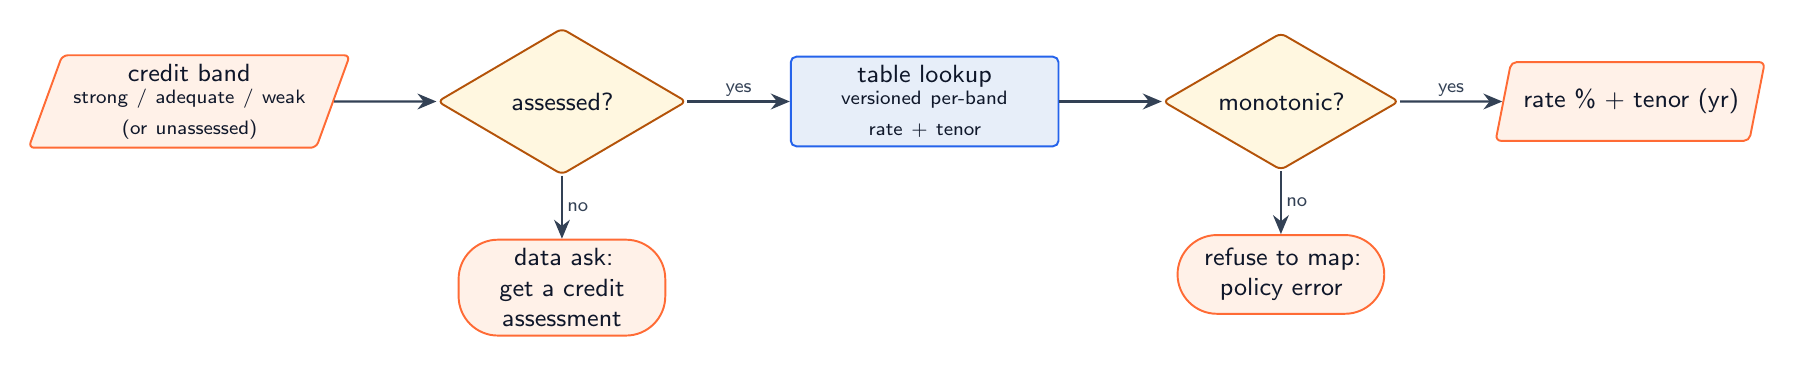
\begin{tikzpicture}[node distance=6mm and 13mm]
  \node[io] (band) {credit band\\\scriptsize strong / adequate / weak\\\scriptsize (or unassessed)};
  \node[decide, right=of band] (assessed) {assessed?};
  \node[proc, right=of assessed, text width=30mm] (lookup) {table lookup\\\scriptsize versioned per-band\\\scriptsize rate + tenor};
  \node[decide, right=of lookup, text width=24mm] (mono) {monotonic?};
  \node[io, right=of mono, text width=28mm] (rt) {rate \% + tenor (yr)};
  \node[term, below=8mm of assessed, fill=nodeIO, draw=nodeIOBd] (ask) {data ask:\\get a credit\\assessment};
  \node[term, below=8mm of mono, fill=nodeIO, draw=nodeIOBd] (refuse) {refuse to map:\\policy error};

  \draw[flow] (band) -- (assessed);
  \draw[flow] (assessed) -- node[flowlabel,above]{yes} (lookup);
  \draw[flow] (assessed.south) to[out=-90,in=90] node[flowlabel,right]{no} (ask.north);
  \draw[flow] (lookup) -- (mono);
  \draw[flow] (mono) -- node[flowlabel,above]{yes} (rt);
  \draw[flow] (mono.south) to[out=-90,in=90] node[flowlabel,right]{no} (refuse.north);
\end{tikzpicture}}
\caption{The deterministic credit mapping. An unassessed counterparty becomes a data ask, never the worst band by default; a non-monotonic policy table is refused outright rather than allowed to produce a flattering loan.}
\label{fig:credit}
\end{figure}

Three rules make this safe:

\begin{itemize}
  \item \textbf{No band is ever invented.} An \emph{unknown} or \emph{not-assessed} counterparty is not quietly defaulted to the worst band (that would fabricate an assessment) nor to a kind one. It produces no rate or tenor and becomes a ranked data ask: ``get a credit assessment''.
  \item \textbf{Monotonicity is enforced.} A worse credit band must never buy a cheaper or longer loan. The model checks that, as the band worsens from strong to weak, the rate never falls and the tenor never lengthens. A policy table that violates this is \emph{refused} -- the mapping returns nothing rather than emit, in the brief's words, ``a glowing return at a rate the covenant does not justify''.
  \item \textbf{The numbers are versioned credit policy.} The rate/tenor table lives in the library, not in code, and is placeholder policy until confirmed, so any credit-driven case is marked not bankable until those values are signed off. The mapping is a pure function of the band and the library: rounded at parse time, it reproduces identical debt terms and an identical provenance hash for identical inputs.
\end{itemize}

The mapping also notes, but does not silently fix, a debt tenor that runs longer than the counterparty's expected contract term, because a loan should not outlast the income that services it. That auto-capping is a financing-policy decision deferred until it can be sourced from the library.

\section{Assembling the case, and why it is never bankable today}

Finally the model packs everything into a \code{FinancialCase}: the two cashflow series, the DSCR summary, the two IRRs, payback, the debt assumptions actually used, the price recommendation, the covenant verdict and the deduplicated warnings. It stamps the run with a provenance context (a hash of the timestamp-free inputs plus the assumption, schema and code versions) so the same request reproduces the same case, and the case identifier is derived from that hash rather than from the clock.

The case is marked \textbf{bankable only if every one of four conditions holds}: the cashflows are bankable (a bankable-candidate result built on no unconfirmed assumption), the DSCR is actually available, the covenant passes, and the covenant assumption is itself confirmed. On the current placeholder assumption sets this is \emph{always false}, and the model says so explicitly: the early releases carry no gearing at all (so the DSCR is unavailable), and \code{gb\_v1\_1}, whose placeholder gearing lets the DSCR compute and the covenant gate genuinely fire, is built entirely of labelled placeholders, so the first condition can never hold on it. That is the platform's safety property at work, not a defect: placeholder numbers must never masquerade as bankable ones.

\begin{rebuild}
To re-implement the financial model and credit mapping from scratch:
\begin{enumerate}
  \item \textbf{Gate.} Read the chosen power from the result. If it is missing or non-positive, raise an ``insufficient inputs'' error; the caller turns that into a ranked data ask. Never invent a system.
  \item \textbf{Revenue.} Sum the per-stream annual revenue for streams whose firmness is firm or contracted only. Hold conditional streams and the separate gated-upside list out of the floor. Warn if the floor is empty (cost-only case).
  \item \textbf{Capex.} power (MW) $\times$ installed-cost rate (\pounds/MW, from the library) $\times$ scenario cost multiplier. Reject negatives. Warn (never block, never alter) if the unit cost is outside the library's benchmark band.
  \item \textbf{Cost lines.} Build each line in Table~\ref{tab:costlines} from its single named assumption (levies from the site tariff). A line with a missing driver is \emph{unavailable} with a warning, never zero, never guessed.
  \item \textbf{P50/P90.} Per operating year: P50 revenue $=$ basis revenue $\times$ price multiplier $\times$ $(1-\text{fade})^{\,year-1}$; P90 revenue $=$ P50 $\times$ $(1-\text{haircut})$. Costs identical in both. EBITDA $=$ revenue $-$ dispatch cost $-$ operating cost. Prefix year 0 $= -$capex. Invariant: P90 $\le$ P50 always.
  \item \textbf{Debt + DSCR.} Need gearing, rate, tenor. Principal $=$ capex $\times$ gearing. Debt service by the recorded sculpting basis: level-payment annuity (default), or a P90-DSCR sculpt -- solve the flat target $x$ with PV(P90 cashflow $\div$ $x$, debt rate, tenor) $=$ principal and set service$_y$ $=$ P90 cashflow$_y$ $\div$ $x$; fall back to the annuity with a warning when a P90 year within the tenor is non-positive or the horizon is shorter than the tenor, and record the basis actually applied. DSCR per year $=$ P90 cashflow $\div$ debt service (skip zero-service years). Minimum DSCR is the headline. Compare to the covenant for a pass/fail. If any of gearing/rate/tenor is missing, report DSCR \emph{unavailable} with a naming warning; never guess.
  \item \textbf{Returns.} Payback $=$ interpolated zero-crossing of cumulative P50 cashflow (``does not pay back'' if it never crosses). Project IRR by bisection \emph{only} for a single-sign-change series. Equity IRR on P50 net of the exact debt service from the DSCR step, same reliability gate.
  \item \textbf{Price.} For fixed \pounds/kWh: revenue requirement $=$ capex $\times$ capital-recovery-factor(target return, horizon) $+$ annual opex; price $=$ requirement $\div$ annual delivered energy. Compute only when target return, capex, opex, horizon and delivered energy are all present. Only assert ``hits target'' on a confirmed target. Savings-share and capacity-fee return shape but no value.
  \item \textbf{Credit map.} Map strong/adequate/weak to (rate, tenor) from the versioned per-band table. Unassessed $\rightarrow$ data ask, never a default band. Enforce monotonicity (worse band: rate non-decreasing, tenor non-increasing); refuse a non-monotonic table. Round at parse time for determinism.
  \item \textbf{Assemble + stamp.} Pack the \code{FinancialCase}; stamp a timestamp-free provenance hash with the assumption / schema / code versions. Mark bankable only if cashflows bankable AND DSCR available AND covenant passes AND covenant assumption confirmed -- otherwise not bankable, with a warning.
  \item \textbf{Test.} The case validates; both series present and P90 $\le$ P50; DSCR unavailable when debt inputs are missing; placeholder assumptions raise warnings; outputs scale when a library value changes (no hidden constants); identical inputs give an identical case (determinism); negative capex rejected; the credit map refuses a non-monotonic table and never defaults an unassessed band.
\end{enumerate}
\end{rebuild}

\begin{keyidea}[The one thing to remember]
This module is pure arithmetic with two firm reflexes. It \emph{underwrites to the downside}: debt is sized and covered on the P90 case while returns are reported on P50. And it \emph{degrades honestly}: a missing input becomes an explicit unavailable field and a warning, an unscored counterparty becomes a data ask, a policy that would flatter a weak borrower is refused, and a run built on placeholders is never marked bankable. No AI authors any number here, and no number is ever invented to fill a gap.
\end{keyidea}

\chapter{The quote lifecycle and run assembly}
\label{ch:quotes}

\modtag{X.2}{Quote lifecycle and assembly}{Deterministic core, traceability anchor}

Everything before this chapter computes a piece of the answer. The site model holds the validated site, the engine chooses a battery size and a half-hourly dispatch, the financial model turns that dispatch into cashflows and a debt-cover figure. This chapter is where those pieces are bound together into a single object and frozen: the \emph{quote record}. It is the artifact the whole pipeline converges on. The three documents the platform exists to produce -- the system specification, the underwriting pack, and the customer proposal -- are all rendered from one quote record, which is precisely why they cannot disagree.

A quote record is two things at once. It is an \textbf{immutable, traceable snapshot}: it carries a hash of the inputs that produced it and the versions of every assumption and every piece of code involved, so any number in it can be traced back to its origin. And it is a \textbf{lifecycle object}: the same deal is represented by a chain of these snapshots as it matures from a rough draft to an operating asset, and each step forward preserves the one before it rather than overwriting it.

\begin{plainnote}
Think of a quote record as a sealed envelope. Inside is the full calculation for one battery at one site, together with a label that says exactly which prices, rules, and software produced it. You never edit what is inside an envelope. If the world changes, you seal a fresh envelope and keep the old one. The platform calls sealing an envelope ``repricing'', and it is the only honest way to change a quote.
\end{plainnote}

\pipelinepos{receives a validated \code{SiteModel} (Ch.~\ref{ch:contracts}), runs it through the engine (Ch.~\ref{ch:engine}--\ref{ch:sizing}) and the financial model (Ch.~\ref{ch:finance}); hands a stamped \code{QuoteRecord} and a \code{TelemetryEvent} (Ch.~\ref{ch:telemetry}) to the outputs renderer (Ch.~\ref{ch:outputs}) and the CLI (Ch.~\ref{ch:cli}).}

\begin{contract}
\textbf{Inputs} (domain objects only -- no files, no clock-dependent state):
\begin{itemize}
  \item a validated, graded \code{SiteModel} (carries its data tier and its ranked list of missing-data asks);
  \item a versioned assumption library (every price, rate, and threshold, with a version string);
  \item an optimisation engine satisfying the standard interface (defaults to the integration-only baseline engine);
  \item optional run context: a scenario set, a forecast reference, an expiry date, a starting lifecycle state, and measured telemetry (contributor, human minutes, installer iterations).
\end{itemize}
\textbf{Outputs:}
\begin{itemize}
  \item one \code{QuoteRecord} -- immutable, hashed, version-stamped, carrying the optimisation result, the financial case (or \code{None} if it could not be priced), the additive output extras, the lifecycle state and history, and honest warnings;
  \item one \code{TelemetryEvent} describing how the quote was produced;
  \item a bundled run result tying the quote, its telemetry, and the underlying detail together for the caller.
\end{itemize}
\end{contract}

\section{One orchestrating run that degrades honestly}

A single function drives one quote from end to end. It takes a site and an assumption library (plus the optional run context above) and returns one bundled result. It exists so that the whole pricing path can be exercised with domain objects alone, with no file reading and no presentation logic: those live in the CLI (Ch.~\ref{ch:cli}). Keeping the orchestrator file-free is what makes the pricing path testable and deterministic.

The run chains four stages in a fixed order:

\begin{enumerate}
  \item \textbf{Engine.} Build an optimisation request from the site, the assumptions, and the chosen scenario set, then solve it. The result is the chosen battery size, its half-hourly dispatch, and the value attributed to each income stream. The engine is injected through the standard interface, so the real dispatch and sizing optimiser slots in behind it unchanged; by default an integration-only baseline engine holds the seam.
  \item \textbf{Finance.} Run the financial model over the site and the optimisation result to produce the financial case: P50/P90 cashflows (a normal year and a conservative bad year), the debt-cover ratio (DSCR, how comfortably cash covers loan repayments; see Appendix~\ref{app:glossary}), the cost lines, and the price that hits the target return.
  \item \textbf{Assemble.} Bind the site, the optimisation result, and the financial case into one \code{QuoteRecord} and stamp it with provenance (Ch.~\ref{ch:provenance}).
  \item \textbf{Telemetry.} Emit one \code{TelemetryEvent} recording how the quote was produced (Ch.~\ref{ch:telemetry}).
\end{enumerate}

The defining property of this run is that it \emph{always answers}. The platform never refuses to produce a quote just because the data is thin. The honest-degradation branch sits at the finance stage: if the financial model has no positive sizing to price, it raises an ``insufficient inputs'' error. The orchestrator catches that error, sets the financial case to \code{None}, marks the quote \emph{not bankable}, and appends an honest warning that names the missing inputs and points to the ranked data asks. The quote is still assembled and still stamped. It simply carries no priced case and says so plainly, rather than inventing a system to fill the gap.

\begin{keyidea}[Always answer, never pretend]
A run that cannot be priced still produces a complete, stamped quote record -- marked not bankable, carrying the financial case as absent, and listing the data that would most improve it. ``Degrade honestly'' is not a fallback bolted on at the edges; it is a branch inside the one orchestrating run, so a quote is never simply a failure.
\end{keyidea}

\subsection{The additive output extras}

Beyond the core binding (site, result, finance), the orchestrator gathers three optional extras for the documents downstream. These are \emph{additive}: they enrich the outputs but never feed the quote's identity hash, so a quote with them and a quote without them that share the same priced inputs share the same identity.

\begin{itemize}
  \item \textbf{The evaluated sizing grid} -- every power-by-duration candidate the sizing search evaluated plus the chosen optimum, for the three-dimensional sizing surface in the proposal.
  \item \textbf{A representative dispatch day} -- one day of half-hourly charge and discharge, for the dispatch chart.
  \item \textbf{The Low / Central / High sensitivities} -- the DSCR and return under each scenario.
\end{itemize}

The first two are read from the engine through optional hooks: a production engine exposes them, the baseline engine does not, and an engine without a hook simply leaves the extra absent with no downstream effect. The sensitivities are computed only when there is a priced base case, because a sensitivity is nothing more than the financial model re-run under a scenario. There is no new financial maths in this layer: each Low/Central/High row re-runs the same deterministic model against the same debt and the same dispatch, recording that scenario's minimum DSCR and its levered (equity) return, and carrying the scenario's months of delay to the commercial operations date so consenting-timeline shifts are reported, not silently applied. The central row reproduces the base case by construction. A figure a scenario cannot support (for example a DSCR when there is no debt) is left absent, never guessed.

\begin{caution}[Dispatch energy and debt are never invented]
Two inputs the financial model would like are never conjured from the library. The annual charge/discharge volumes that switch on levies-on-charge and the price-to-target line are read from the engine through an optional hook (or supplied explicitly); the placeholder engine has neither, so those lines stay honestly unavailable. Debt terms (rate, tenor, covenant) are likewise only ever supplied explicitly by a deliberate, labelled caller such as the opt-in demo, because the placeholder library carries no debt structure. The default omits both, which keeps the honest real-mode path unchanged.
\end{caution}

\begin{figure}[H]
\centering
\resizebox{\textwidth}{!}{%
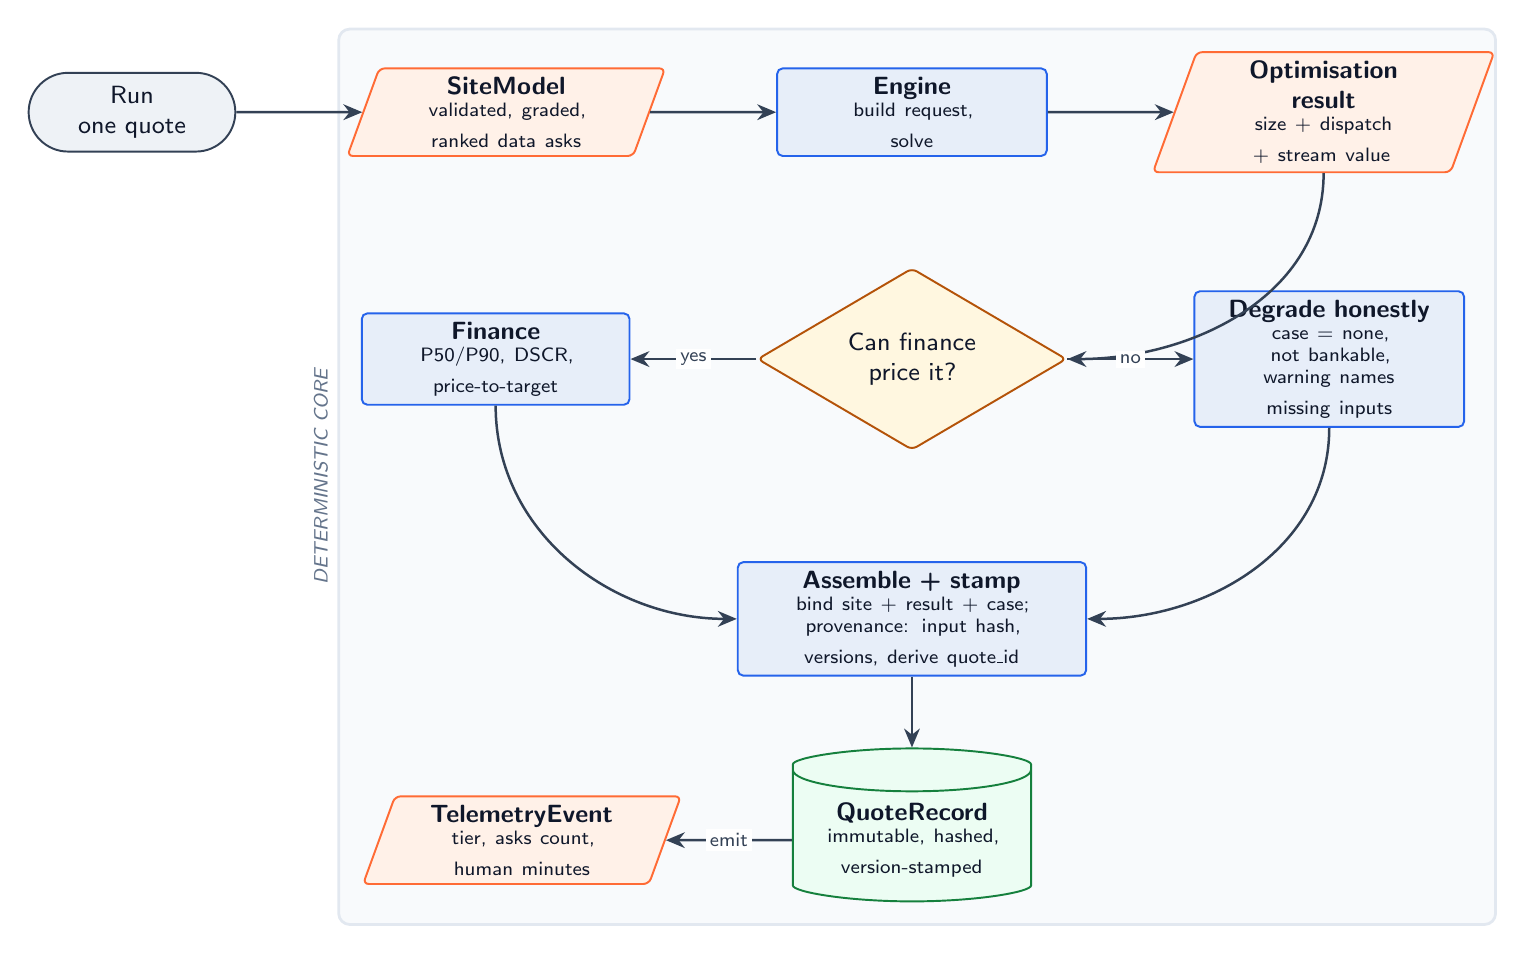
\begin{tikzpicture}[node distance=9mm and 16mm]
  \node[term] (start) {Run\\one quote};
  \node[io, right=of start] (site) {\textbf{SiteModel}\\\scriptsize validated, graded,\\\scriptsize ranked data asks};
  \node[proc, right=of site] (engine) {\textbf{Engine}\\\scriptsize build request,\\\scriptsize solve};
  \node[io, right=of engine] (optres) {\textbf{Optimisation\\result}\\\scriptsize size + dispatch\\\scriptsize + stream value};

  \node[decide, below=14mm of engine] (canprice) {Can finance\\price it?};
  \node[proc, left=of canprice, text width=30mm] (finance) {\textbf{Finance}\\\scriptsize P50/P90, DSCR,\\\scriptsize price-to-target};
  \node[proc, right=of canprice, text width=32mm] (degrade) {\textbf{Degrade honestly}\\\scriptsize case = none,\\\scriptsize not bankable,\\\scriptsize warning names\\\scriptsize missing inputs};

  \node[proc, below=14mm of canprice, minimum width=44mm, text width=42mm] (assemble)
     {\textbf{Assemble + stamp}\\\scriptsize bind site + result + case;\\\scriptsize provenance: input hash,\\\scriptsize versions, derive quote\_id};
  \node[store, below=of assemble] (quote) {\textbf{QuoteRecord}\\\scriptsize immutable, hashed,\\\scriptsize version-stamped};
  \node[io, left=of quote, text width=30mm] (telem) {\textbf{TelemetryEvent}\\\scriptsize tier, asks count,\\\scriptsize human minutes};

  \draw[flow] (start) -- (site);
  \draw[flow] (site) -- (engine);
  \draw[flow] (engine) -- (optres);
  \draw[flow] (optres) to[out=-90,in=0] (canprice.east);
  \draw[flow] (canprice) -- node[flowlabel]{yes} (finance);
  \draw[flow] (canprice) -- node[flowlabel]{no} (degrade);
  \draw[flow] (finance) to[out=-90,in=180] (assemble.west);
  \draw[flow] (degrade) to[out=-90,in=0] (assemble.east);
  \draw[flow] (assemble) -- (quote);
  \draw[flow] (quote) -- node[flowlabel]{emit} (telem);

  \begin{scope}[on background layer]
    \node[groupbox, fit=(site)(engine)(optres)(canprice)(finance)(degrade)(assemble)(quote),
          inner sep=8pt, label={[note,rotate=90,anchor=south]west:DETERMINISTIC CORE}] {};
  \end{scope}
\end{tikzpicture}}
\caption{The one orchestrating run. Engine then finance then assemble then telemetry, with the honest-degradation branch at the finance gate: when finance cannot price the run, the quote is still produced -- marked not bankable, with the financial case absent and a warning naming the missing inputs.}
\label{fig:quote-run}
\end{figure}

\section{What the quote record binds}

The assembly step is the join point of the pipeline. It is deliberately free of pricing or optimisation logic and of heavy data libraries: it only reflects what the run produced and stamps it. It builds a canonical, timestamp-free description of the run, asks the provenance layer (Ch.~\ref{ch:provenance}) to hash it and stamp the versions, derives the quote's identity from that, and writes the record.

Table~\ref{tab:quoterecord} lists what one record binds. The grouping matters: the first block is \emph{identity and traceability}, the second is the \emph{computed answer}, the third is the \emph{additive extras for the documents}, and the last is \emph{lifecycle and honesty}.

\begin{table}[H]
\centering
\caption{The fields a quote record binds, grouped by role.}
\label{tab:quoterecord}
\small\sffamily
\begin{tabularx}{\textwidth}{@{}l L L@{}}
\toprule
\textbf{Field} & \textbf{What it is} & \textbf{Why it is here} \\
\midrule
\multicolumn{3}{@{}l}{\textit{Identity and traceability}}\\
quote id & Deterministic id derived from the run context. & Identical priced inputs give an identical id. \\
input hash & Hash of the canonical, timestamp-free run input. & Pins the exact site, result, case, assumption version, and forecast content. \\
assumption version & The version string of the library used. & A quote is valid only against this version. \\
code / schema version & The software and contract versions. & Lets any answer be reproduced or attributed. \\
output hash & Hash of the record's own content. & Detects any later tampering with the saved record (Ch.~\ref{ch:provenance}). \\
created\_at & Timestamp. & Metadata only; deliberately excluded from every hash. \\
\midrule
\multicolumn{3}{@{}l}{\textit{The computed answer}}\\
site id & Which site this is for. & The link back to the validated input. \\
data tier & T0--T2, copied from the site. & Grades how much the answer can be trusted. \\
optimisation result & The chosen size, dispatch, and stream value. & The engine's frozen output. \\
financial case & Cashflows, DSCR, costs, price-to-target. & The finance output; \code{None} on a degraded run. \\
\midrule
\multicolumn{3}{@{}l}{\textit{Additive extras for the documents}}\\
sizing grid & Every evaluated size plus the optimum. & The three-dimensional sizing surface; absent if the engine has no hook. \\
dispatch profile & A representative half-hourly day. & The dispatch chart; absent if unavailable. \\
sensitivities & Low/Central/High DSCR and return rows. & The Output-2 sensitivity table; empty if not priced. \\
\midrule
\multicolumn{3}{@{}l}{\textit{Lifecycle and honesty}}\\
quote mode & The current lifecycle state. & Where the deal is on its path. \\
status history & The ordered prior states. & The trajectory, append-only. \\
expiry date & Optional validity date. & When the snapshot lapses. \\
warnings & Aggregated honest notes. & Gate, consent, credit, missing-data, and not-bankable asks. \\
\bottomrule
\end{tabularx}
\end{table}

\subsection{Identity is content, not the clock}

The quote's identity is computed from \emph{what the run says}, never from \emph{when it ran}. The canonical run input is built by serialising the site, the optimisation result, and the financial case to plain JSON (enumerations become their values, dates become ISO strings), then adding the assumption version and the forecast's content hash. Two things are deliberately left out. The top-level \code{created\_at} timestamp is excluded everywhere, because a timestamp is metadata and must never feed a computed identity; otherwise the same run on two different days would get two different ids. And the forecast is pinned by its content hash alone, never by the whole forecast reference object, whose ``verified'' flag and warnings change over time and would make the pin non-reproducible.

That canonical input is handed to the provenance layer, which returns the input hash, the stamped versions, and a deterministic run id. The quote id is that run id with a \code{quote\_} prefix. The consequence is the determinism guarantee made flesh: identical inputs, the same assumption version, and the same code produce an identical quote id, every time, on every machine.

\begin{keyidea}[The hash is over the run, not the record]
Assembly hashes the \emph{run inputs} (site, result, case, versions, forecast content), not the saved record. That is why the additive extras -- the sizing grid, the dispatch profile, the sensitivities -- can be attached without changing the input hash or the quote id. They are downstream conveniences, not part of what makes the answer what it is. Adding them is backward-compatible: an older quote saved without them validates unchanged.
\end{keyidea}

\subsection{Honest warnings, gathered from every layer}

The record's warnings are aggregated and de-duplicated from the whole run, preserving order. They collect the optimisation result's own warnings, the financial case's warnings (when there is one), a note when the site still has ranked data asks outstanding, any caller-supplied notes (for example an HH or forecast file that could not be used), and -- whenever the result is anything other than a bankable candidate -- the standard not-bankable disclaimer. That disclaimer states plainly that the quote is indicative only, uses placeholder assumptions and/or has no established debt case, and must not be presented to capital as bankable. On the current placeholder assumption set every quote carries it, which is the intended safety property: a placeholder must never masquerade as a bankable number.

\section{The lifecycle: matured by snapshots, never edits}

A quote is a long-lived object, not a one-off printout. The same deal advances through a fixed, strictly sequential chain of states as it matures:

\begin{center}\sffamily\small
draft $\;\rightarrow\;$ indicative $\;\rightarrow\;$ underwritten $\;\rightarrow\;$ contracted $\;\rightarrow\;$ operating
\end{center}

Each state means roughly: \emph{draft}, a first pass; \emph{indicative}, shareable with the customer; \emph{underwritten}, fit for a lender's review; \emph{contracted}, the deal is signed; \emph{operating}, the asset is live. From any live state a quote may also \emph{lapse}, which is terminal. The chain only moves forward one step at a time: there is no skipping ahead and no reversing in this version.

The rule that makes the lifecycle trustworthy is that \textbf{advancing never mutates}. Each transition produces a \emph{new} validated record. The outgoing state is appended to the status history and the mode is advanced to the new state; prior history entries are never touched. By convention the history holds only \emph{prior} states, and the current state lives in the mode field and is not duplicated in the history. So the full trajectory of a quote is always reconstructable from its history plus its current mode, and no earlier snapshot is ever changed under it.

A transition is rejected if it is not one of the legal moves from the current state. Each live state permits exactly its single forward step plus a lapse; a terminal state permits nothing. An illegal request (a skip or a reverse) raises an invalid-transition error that names what was allowed. Crucially, a transition rebuilds the record through full schema re-validation rather than a shallow copy, so the schema's invariants re-fire on every step. The most important of these guards an underwritten quote built from a coarse T0 site: it is only allowed if the record carries an explicit validation warning, because T0 data (annual energy, tariff, and postcode only) is too thin to underwrite firmly. A shallow copy would silently skip that check; re-validation does not.

\begin{figure}[H]
\centering
\resizebox{\textwidth}{!}{%
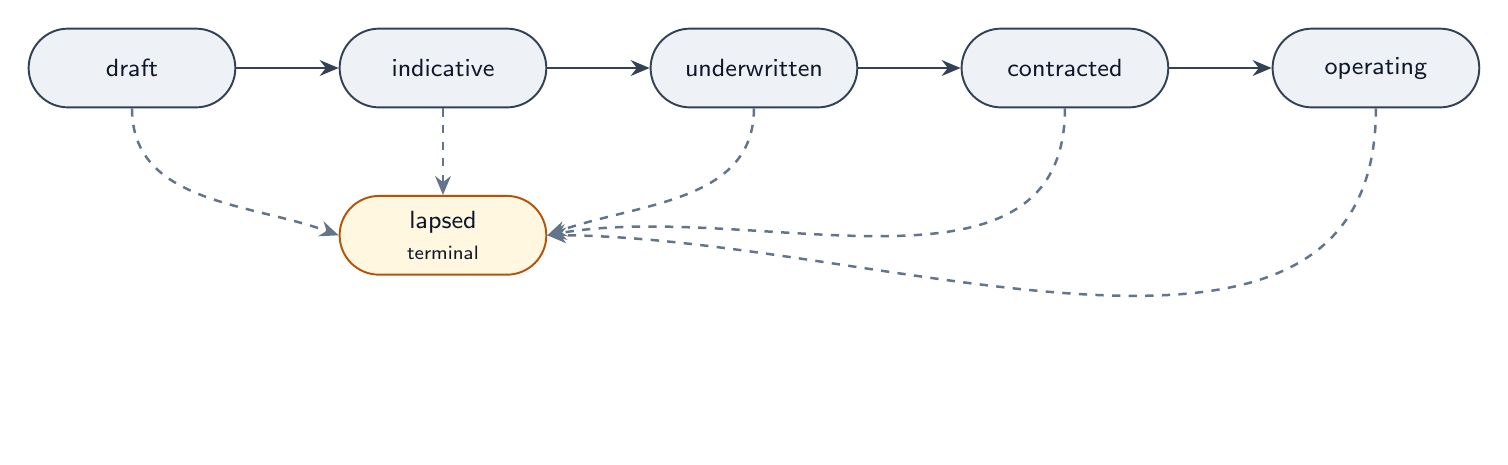
\begin{tikzpicture}[node distance=7mm and 13mm]
  \node[term] (draft) {draft};
  \node[term, right=of draft] (indic) {indicative};
  \node[term, right=of indic] (under) {underwritten};
  \node[term, right=of under] (contr) {contracted};
  \node[term, right=of contr] (oper) {operating};
  \node[term, below=11mm of indic, fill=nodeDecision, draw=nodeDecisionBd] (lapsed) {lapsed\\\scriptsize terminal};

  \draw[flow] (draft) -- (indic);
  \draw[flow] (indic) -- (under);
  \draw[flow] (under) -- (contr);
  \draw[flow] (contr) -- (oper);

  \draw[flowback] (draft.south) to[out=-90,in=160] (lapsed.west);
  \draw[flowback] (indic.south) -- (lapsed.north);
  \draw[flowback] (under.south) to[out=-90,in=20] (lapsed.east);
  \draw[flowback] (contr.south) to[out=-90,in=10] (lapsed.east);
  \draw[flowback] (oper.south) to[out=-90,in=0] (lapsed.east);
\end{tikzpicture}}
\caption{The quote lifecycle. The forward chain advances one strict step at a time (solid); from any live state the quote may lapse (dashed), which is terminal. Each forward step produces a new immutable snapshot and appends the outgoing state to the history.}
\label{fig:quote-lifecycle}
\end{figure}

\subsection{Valid only against the version that produced it}

A quote record pins the assumption version and the code version that produced it, and those versions do not float. The quote is valid \emph{only} against them. If a material assumption changes beyond tolerance -- a tariff updates, a cost line moves, a covenant tightens -- the correct response is to \textbf{reprice}: run the orchestrator again to produce a fresh snapshot, stamped with the new version, and keep the old one in the trail. The wrong response is to reach into an existing record and edit a number, because that would break the chain from the figure back to the inputs and versions that justify it. Reprice, never silently edit.

\begin{caution}[A material change triggers a reprice, not an edit]
Because identity is a pure function of the inputs and versions, a repriced quote that genuinely differs gets a new quote id automatically, and one that does not differ resolves to the same id. There is no supported path that changes a bound number in place. If you find yourself wanting to ``just tweak'' a figure on an issued quote, that is the signal to reprice.
\end{caution}

\section{Where this sits in the manual}

This chapter is the centre of traceability, and it leans on two siblings. The provenance layer (Ch.~\ref{ch:provenance}) owns the hashing and version stamping that assembly calls; this chapter only decides \emph{what} is hashed (the canonical run input) and \emph{how} the result is bound. The telemetry chapter (Ch.~\ref{ch:telemetry}) owns the event emitted per run; this chapter only triggers it. The financial case it binds comes from Ch.~\ref{ch:finance}, the additive extras feed the documents in Ch.~\ref{ch:outputs}, and the whole orchestrating run is what the command-line tool calls in Ch.~\ref{ch:cli}.

\begin{rebuild}[How to rebuild the quote layer]
\begin{enumerate}
  \item \textbf{Define the record shape.} A model that forbids unknown fields, carrying: \code{quote\_id}, \code{quote\_mode}; \code{site\_id}, \code{data\_tier}; \code{input\_hash}, \code{assumption\_version}, \code{code\_version} (all optional, populated at assembly); the optimisation result and the financial case (the case optional); the additive \code{sizing\_grid}, \code{dispatch\_profile}, and a list of scenario sensitivities (all defaulting to absent/empty); an optional \code{expiry\_date}; a \code{status\_history} list and a \code{warnings} list (both defaulting to empty); and a \code{created\_at} timestamp. Add one validator: an underwritten quote from a T0 site must carry at least one warning.
  \item \textbf{Write the canonical run input.} A function returning a dict: the site and the optimisation result each serialised to JSON with \code{created\_at} excluded; the financial case serialised to JSON or \code{None}; the assumption version; and the forecast's content hash or \code{None}. No timestamps, no whole forecast object.
  \item \textbf{Write assembly.} Build a run context over that canonical input (passing the assumption and schema versions), copy its input hash and versions onto the record, set \code{quote\_id} to the run id with a \code{quote\_} prefix, and aggregate de-duplicated warnings from the result, the case, the site's outstanding asks, any caller notes, and the not-bankable disclaimer whenever the result is not a bankable candidate. Default the lifecycle state to draft.
  \item \textbf{Write the orchestrator.} Take domain objects only. Build the request and solve via the injected engine (default the baseline). Read the optional dispatch-energy, sizing-grid, and dispatch-profile hooks if present. Run the financial model; on an insufficient-inputs error, set the case to \code{None}, mark not bankable, and append a warning naming the missing inputs. Compute sensitivities only when a case exists. Assemble, emit telemetry, and return the bundle.
  \item \textbf{Write the lifecycle.} A forward map (draft to indicative to underwritten to contracted to operating) plus a lapse from every live state and nothing from the terminal lapsed state. A transition appends the outgoing state to the history, advances the mode, and re-validates the whole record (not a shallow copy) so the T0 guard re-fires; reject any move not in the legal set.
  \item \textbf{What to test.} Identical inputs give an identical quote id; changing only \code{created\_at} does not change the id; a missing financial case yields a not-bankable quote with the data-asks warning; the additive extras do not change the input hash; legal transitions produce a new snapshot and preserve prior history; illegal skips/reverses are rejected; and an underwritten T0 quote without a warning is rejected.
\end{enumerate}
\end{rebuild}

\chapter{Telemetry and the cost-compression benchmark}
\label{ch:telemetry}
\modtag{X.3}{Telemetry and benchmark}{Cross-cutting}

The platform is built on a claim: that it produces a quote faster and cheaper than a person can build one by hand, without losing trust. A claim like that is worth nothing unless it can be checked with numbers. This module is the part of the system that makes the claim \emph{measurable rather than asserted}. Every run leaves a small, structured record of how it was produced -- the quality of the data it started from, the human time it cost, the back-and-forth it took, and how the deal eventually turned out. Those records accumulate into one dataset that can be summarised and, in principle, disproved.

There are two kinds of row in that dataset. The first is the ordinary one: a record emitted by the system every time it makes a quote. The second is the \emph{control group}: a small set of measurements of what a quote costs \emph{today}, built by hand, captured before the system makes hand-building a thing of the past. Without that ``before'' picture there is nothing to compress against. This chapter covers both, the analytics that compare them, and the reason the measurement has to ship with the very first quote rather than being added later.

\pipelinepos{reads the assembled \code{QuoteRecord} and the populated \code{SiteModel} produced by the lifecycle module (Ch.~\ref{ch:quotes}), which carries the data tier graded at intake (Ch.~\ref{ch:ingestion}); emits one telemetry event per run into an append-only store, alongside the manual benchmark, and feeds the whole store to the analytics summary.}

\begin{contract}[Inputs and outputs]
\textbf{In (per system run):} the assembled \code{QuoteRecord} (its quote identifier, its data tier, and -- by reference -- its version stamps); the populated \code{SiteModel} (whose outstanding data asks give the missing-data count); and optional \emph{measured} inputs supplied by the caller: the contributor, human minutes, installer iterations, the commercial outcome and its reason, and a realised-vs-underwritten percentage once known. \\[3pt]
\textbf{In (the benchmark, captured once per hand-built quote):} a manual benchmark record -- site, contributor, date, data tier, measured human minutes, iteration count, the categories of missing data chased, the artifact type, and the outcome. \\[3pt]
\textbf{Out:} one append-only \textbf{telemetry event} per run, and a converted event per benchmark, living in \emph{one} dataset; and a \textbf{telemetry summary} aggregating that dataset into the cost-compression metrics. No number here ever feeds a price.
\end{contract}

\section{The telemetry event: one row per run}

The unit of the dataset is a single \emph{telemetry event}: a flat, append-only record describing one moment in a quote's life. It is deliberately small and deliberately separate from the priced numbers. It records \emph{how} a quote was produced, never \emph{what} it priced. Table~\ref{tab:event} lists its fields.

\begin{table}[H]
\centering
\caption{The fields of a telemetry event. Every field except the identifiers and the event type is optional, because honest measurement means leaving a value blank until it is genuinely known rather than guessing it.}
\label{tab:event}
\small\sffamily
\begin{tabularx}{\textwidth}{@{}l l L@{}}
\toprule
\textbf{Field} & \textbf{Type} & \textbf{Meaning} \\
\midrule
event id & string & Stable identifier for this row, by default the quote id joined to the event type. \\
quote id & string & Which quote this event belongs to. For a system run it is the \code{QuoteRecord} id; for a benchmark it is the linked system quote if one exists, else a stable \code{manual:<id>}. \\
event type & string & The discriminator. \code{quote\_created} for a system run, \code{manual\_benchmark} for a hand-built baseline. \\
data tier & T0--T2 / none & The data quality at intake (Ch.~\ref{ch:ingestion}), copied off the quote. The axis the hit-rate is broken down by. \\
human minutes & number $\ge 0$ / none & Total wall-clock effort across all people. Left blank on a system run until measured; required and positive on a benchmark. \\
contributor & string / none & Who did the work. \\
installer iterations & integer $\ge 0$ / none & Rounds of back-and-forth with the installer or customer to get usable data. \\
missing data count & integer $\ge 0$ / none & How many ranked data asks were still outstanding at quote time, read off the populated site. \\
outcome & enum & The commercial result: pending, sent, won, lost, abandoned. Defaults to \emph{pending}, because a fresh quote has no result yet. \\
outcome reason & string / none & Free text explaining a win or a loss. Blank until known. \\
realised vs underwritten \% & number / none & Realised performance as a percentage of the underwritten figure. Blank until measurement and verification supplies a real number. \\
notes & string / none & Free-text context. \\
created at & timestamp & When the event was recorded. Metadata only; it never enters a computed number. \\
schema version & string & The shape version stamped on every record in the system. \\
\bottomrule
\end{tabularx}
\end{table}

A few fields carry the weight of the chapter and deserve explaining.

\textbf{Data tier} is the link to the quality of the inputs. It is graded at intake (T0 coarse, T1 partial, T2 a full validated year; see Ch.~\ref{ch:ingestion}) and simply copied onto the event. It is the axis the analytics slice the hit-rate by, so the platform can ask whether thin-data quotes win at a different rate than full-data ones.

\textbf{Human minutes} is the headline cost number. It is the \emph{total} wall-clock effort across everyone who touched the quote, not one person's time. On a system run it is optional, left blank until someone actually measures it, never invented. On a benchmark it is required and must be positive: a benchmark with no recorded effort is not a benchmark.

\textbf{Missing data count} is taken from the \emph{populated} site, after ingestion has attached its ranked list of the data that would most improve the quote (Ch.~\ref{ch:ingestion}). It records how many asks were still outstanding when the quote was made, so a thin quote and a complete one are distinguishable in the data.

\textbf{Outcome} and its \textbf{reason} are the hit-rate axis. A fresh quote is \emph{pending}; it becomes won or lost only when the deal resolves, at which point the reason explains why. \textbf{Realised vs underwritten} closes the loop much later: after the system is built and operating, measurement and verification reports what the battery actually earned, expressed as a percentage of what was underwritten. It stays blank -- never zero, never a guess -- until a real figure exists.

\paragraph{Version stamps live on the record, not the event.} The event itself carries only its own shape version. The full set of stamps that pin a run -- the assumption-set version, the code version, the engine version, the input hash -- lives on the \code{QuoteRecord} the event names by its quote id (Ch.~\ref{ch:quotes} and Ch.~\ref{ch:provenance}). The event references the record rather than copying those stamps, so every metric in the analytics can still be traced back to the exact versions that produced it, while the telemetry row stays small and append-only.

\begin{keyidea}[The event records how, never what]
A telemetry event is pure perimeter measurement. It carries the cost and the outcome of a run; it never carries, and never feeds, a priced number. This is the same hard wall that runs through the whole platform: prose is drafted, numbers are computed, and measurement sits to one side of both.
\end{keyidea}

\subsection{Where the event comes from}

When the lifecycle module finishes assembling a quote (Ch.~\ref{ch:quotes}), it emits exactly one telemetry event for the run. The emitter reads the data tier straight off the quote, counts the still-outstanding asks off the populated site, and copies through any measured inputs the caller passed (contributor, human minutes, iterations). It does not compute anything: it is a faithful snapshot of the run as it happened. The result is a \code{quote\_created} event, ready to append to the store.

\section{The manual benchmark: the control group}

Before the system existed, every quote was built by hand. The cost of \emph{that} -- the human hours, the rounds of chasing an installer for a meter file, the tariff stack rebuilt from a paper bill -- is the baseline the whole cost-compression thesis is measured against. The manual benchmark is the deliberate capture of that baseline.

A \emph{manual benchmark record} is one hand-built quote, measured. Its fields are listed in Table~\ref{tab:benchmark}. Crucially, it records only \emph{real} effort on a \emph{real} quote: over-counting the minutes is acceptable, guessing is not, and any illustrative example must be labelled as such and never treated as a real input.

\begin{table}[H]
\centering
\caption{The fields of a manual benchmark record. It is a strict schema: an unknown or mistyped field is a validation error, and the human-minutes value must be present and positive.}
\label{tab:benchmark}
\small\sffamily
\begin{tabularx}{\textwidth}{@{}l L@{}}
\toprule
\textbf{Field} & \textbf{Meaning} \\
\midrule
benchmark id & Stable identifier for this row. \\
site name & The site label, often with its postcode area. \\
contributor & Who built the quote; minutes are summed across everyone. \\
date & When the hand-built quote was produced. Required, so every row is placeable in time. \\
data tier & The data quality the quote was built from (T0--T2). Required, so every row is placeable by data quality. \\
human minutes & \textbf{Required, positive.} Total wall-clock effort across all people. \\
iterations & Rounds of back-and-forth with the installer or customer. \\
missing data categories & The kinds of data that had to be chased or assumed. \\
source & Provenance of the benchmark; defaults to ``manual quote''. \\
quote type & The artifact the hand-built quote produced (see the caution below). \\
quote outcome & The commercial outcome, drawn from the same vocabulary as a system quote. \\
notes & What explains the time: messy data, manual reconstruction, the tooling used. \\
linked quote id & The system quote this baseline pairs with, once one exists. \\
\bottomrule
\end{tabularx}
\end{table}

A benchmark does not live in its own separate world. It is \emph{converted} into the same telemetry-event shape as a system run, marked with the event type \code{manual\_benchmark}, so the manual baseline and the system quotes sit in one dataset and can be compared apples to apples. The conversion carries across the measured fields -- human minutes, the iteration count (as installer iterations), the count of missing-data categories, the data tier, the contributor, and the outcome -- and derives the event timestamp deterministically from the benchmark date, so the same record always yields the same event. The records can also be rendered as a Markdown table, which is how the running log is kept readable by hand alongside the validated objects.

\begin{caution}[Two words that look the same and are not]
The word \emph{indicative} (and likewise \emph{underwritten}) appears in two unrelated places, and confusing them corrupts the dataset.
\begin{itemize}
  \item A \textbf{quote lifecycle state} (\code{QuoteMode}: draft, indicative, underwritten, contracted, operating, lapsed) describes \emph{how mature a deal is}. It belongs to the \code{QuoteRecord} and travels through the lifecycle (Ch.~\ref{ch:quotes}).
  \item A \textbf{manual-benchmark artifact type} (\code{ManualQuoteType}: indicative, underwritten, proposal, other) describes \emph{what kind of document a single hand-built quote produced}. It belongs only to a benchmark row.
\end{itemize}
They share spellings but are different fields on different objects with different value sets. A benchmark's ``underwritten'' is the type of document a person produced by hand; a quote's ``underwritten'' is a stage in a live deal's life. Never map one onto the other, and never let a benchmark's artifact type be read as a lifecycle state.
\end{caution}

\section{The analytics: what the dataset must answer}

The whole point of collecting events is to summarise them. The summary aggregates a collection of events -- system quotes and benchmarks together -- into the cost-compression metrics. It is pure aggregation: no clock, no randomness, deterministic, so the same dataset always produces the same summary.

The platform is honest about which metrics it can compute today and which it cannot. Two of the four target metrics are computable from the data captured now; two require inputs that do not exist yet, and those are returned as named \emph{unavailable} notes rather than fabricated.

\begin{table}[H]
\centering
\caption{The four target metrics of the cost-compression dataset, and whether they can be computed from what is captured today.}
\label{tab:metrics}
\small\sffamily
\begin{tabularx}{\textwidth}{@{}l c L@{}}
\toprule
\textbf{Metric} & \textbf{Today} & \textbf{How / why not} \\
\midrule
Time-to-quote vs the manual benchmark & yes & The mean human minutes of system runs against the mean of the benchmarks, expressed as a ratio. \\
Hit-rate by data tier & yes & Wins divided by resolved deals, broken down by the data tier at intake. \\
Marginal cost per quote & no & Needs a per-quote cost input that is not captured yet. Returned as an honest unavailable note. \\
Underwriting error by stream & no & Needs realised-vs-underwritten broken down \emph{by income stream}; only a whole-quote realised figure exists, populated after the operation date. \\
\bottomrule
\end{tabularx}
\end{table}

\subsection{Time-to-quote and the compression ratio}

The headline figure is how much faster the system is than a person. The summary takes the mean human minutes across all system runs that have a measured value, and the mean across all benchmarks that have one. The \textbf{compression ratio} is the benchmark mean divided by the system mean:
\[
\text{compression ratio} \;=\; \frac{\text{mean benchmark human minutes}}{\text{mean system human minutes}}.
\]
A ratio above one means the system is faster; a ratio of, say, ten means a system quote costs a tenth of the human time of a hand-built one. The ratio is reported only when both means exist and the system mean is positive; otherwise it is left undefined rather than divided by a missing or zero value.

\begin{plainnote}
The ratio is deliberately a \emph{proxy} for time-to-quote, built from measured human minutes rather than from wall-clock duration. The event shape can also support a true time-to-quote, the gap between an intake event and the quote-created event for the same quote, once both events are routinely logged. Until then the human-minutes proxy is the honest, available measure, and it is labelled as such.
\end{plainnote}

\subsection{Hit-rate by data tier}

The second computable metric asks whether the quality of the input data changes how often a quote is won. The summary looks only at events whose deal has \emph{resolved} -- that is, whose outcome is won or lost; pending, sent and abandoned rows are still in flight and are excluded. For each data tier it counts the wins and the resolved total, and reports
\[
\text{hit-rate}(\text{tier}) \;=\; \frac{\text{wins in tier}}{\text{resolved deals in tier}}.
\]
This is what turns the data-tier label into evidence: it lets the platform see whether T2 (full-data) quotes convert better than T0 (coarse) ones, which is exactly the kind of question the honest-degradation design (Ch.~\ref{ch:ingestion}) needs answered over time.

\subsection{Realised vs underwritten, after the operation date}

The slowest loop to close is the most important one for a lender's trust: did the battery actually earn what was underwritten? That figure cannot exist at quote time. It arrives only after the system is built and running, once measurement and verification reports real performance after the commercial operation date. The event reserves a field for it -- realised performance as a percentage of the underwritten figure -- and leaves it blank until a real number is supplied. The platform is explicit that the finer-grained version of this metric, error broken down \emph{by income stream}, is not yet computable, because only a whole-quote realised figure is captured; it is named as unavailable rather than approximated.

\section{The flow: from each run to the cost-compression metrics}

Figure~\ref{fig:telemetry} draws the whole module. Each system run emits one event; each hand-built quote is captured as a benchmark and converted into the same shape; both land in one append-only store; and the analytics read the store to produce the cost-compression and hit-rate-by-tier figures.

\begin{figure}[H]
\centering
\resizebox{\textwidth}{!}{%
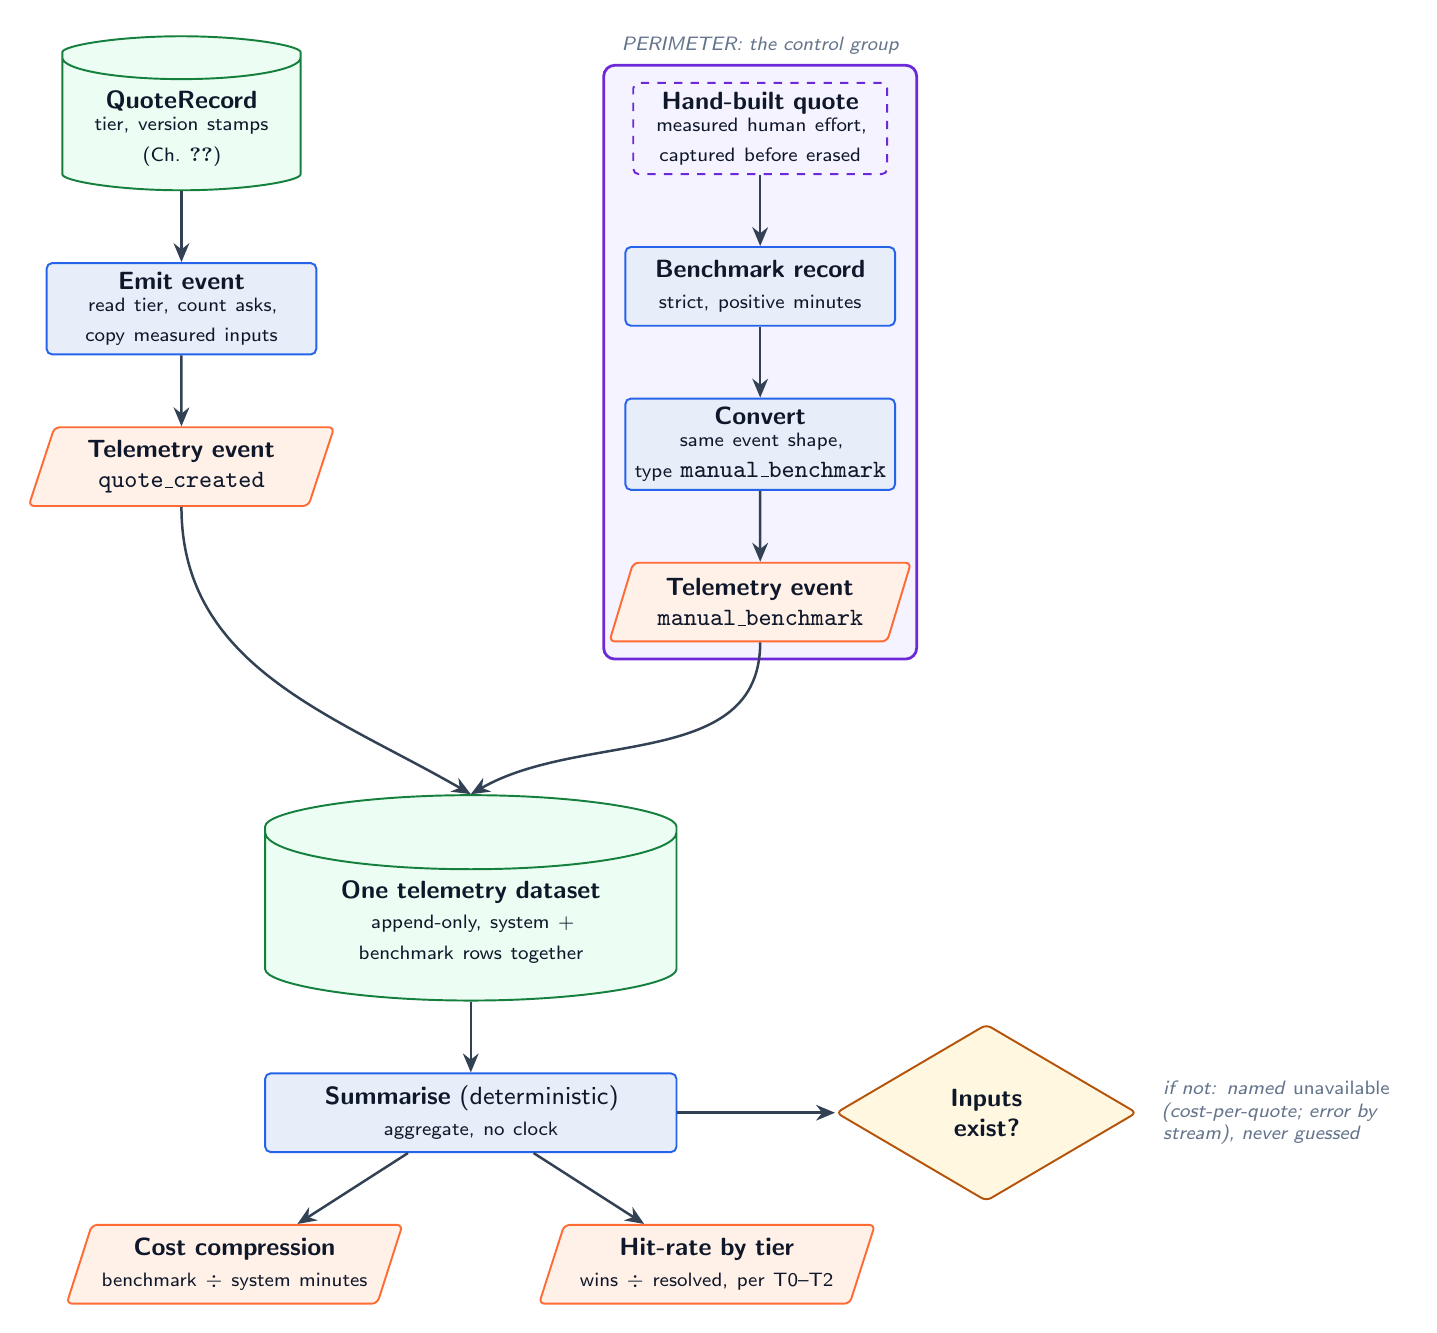
\begin{tikzpicture}[node distance=9mm and 18mm]
  % system side
  \node[store] (quote) {\textbf{QuoteRecord}\\\scriptsize tier, version stamps\\\scriptsize (Ch.~\ref{ch:quotes})};
  \node[proc, below=of quote] (emit) {\textbf{Emit event}\\\scriptsize read tier, count asks,\\\scriptsize copy measured inputs};
  \node[io, below=of emit] (sysev) {\textbf{Telemetry event}\\\scriptsize \code{quote\_created}};

  % benchmark side
  \node[ext, right=42mm of quote] (manual) {\textbf{Hand-built quote}\\\scriptsize measured human effort,\\\scriptsize captured before erased};
  \node[proc, below=of manual] (bench) {\textbf{Benchmark record}\\\scriptsize strict, positive minutes};
  \node[proc, below=of bench] (conv) {\textbf{Convert}\\\scriptsize same event shape,\\\scriptsize type \code{manual\_benchmark}};
  \node[io, below=of conv] (benev) {\textbf{Telemetry event}\\\scriptsize \code{manual\_benchmark}};

  % store
  \node[store, below=33mm of $(sysev)!0.5!(benev)$, minimum width=52mm, text width=50mm] (storeev)
     {\textbf{One telemetry dataset}\\\scriptsize append-only, system + benchmark rows together};

  % analytics
  \node[proc, below=of storeev, minimum width=52mm, text width=50mm] (agg)
     {\textbf{Summarise} (deterministic)\\\scriptsize aggregate, no clock};
  \node[io, below=of agg, xshift=-30mm, text width=34mm] (cc)
     {\textbf{Cost compression}\\\scriptsize benchmark $\div$ system minutes};
  \node[io, below=of agg, xshift=30mm, text width=34mm] (hr)
     {\textbf{Hit-rate by tier}\\\scriptsize wins $\div$ resolved, per T0--T2};
  \node[decide, right=20mm of agg] (un) {\textbf{Inputs\\exist?}};
  \node[note, right=2mm of un, text width=30mm] (note)
     {if not: named \emph{unavailable} (cost-per-quote; error by stream), never guessed};

  % arrows
  \draw[flow] (quote) -- (emit);
  \draw[flow] (emit) -- (sysev);
  \draw[flow] (manual) -- (bench);
  \draw[flow] (bench) -- (conv);
  \draw[flow] (conv) -- (benev);
  \draw[flow] (sysev) to[out=-90,in=150] (storeev.north);
  \draw[flow] (benev) to[out=-90,in=30] (storeev.north);
  \draw[flow] (storeev) -- (agg);
  \draw[flow] (agg) -- (cc);
  \draw[flow] (agg) -- (hr);
  \draw[flow] (agg) -- (un);

  % backdrops
  \begin{scope}[on background layer]
    \node[groupbox, draw=nodeExtBd, fill=gridqVioletBg, fit=(manual)(bench)(conv)(benev), inner sep=6pt,
          label={[note,anchor=south]north:PERIMETER: the control group}] {};
  \end{scope}
\end{tikzpicture}}
\caption{The telemetry module. System runs (left) and hand-built quotes (right, the perimeter control group) become events of one shape in one append-only store. The deterministic summary turns the store into the cost-compression ratio and the hit-rate by data tier; metrics whose inputs do not yet exist are returned as honest unavailable notes rather than guessed.}
\label{fig:telemetry}
\end{figure}

\section{Why telemetry must ship with the first quote}

The single most important property of this module is timing. The benchmark is a \emph{before} picture, and there is exactly one chance to take it: before the system is in use. Retrofitted, the data is worthless as evidence. Nobody can reliably remember, a year on, how many hours a particular hand-built quote took or how many times they chased the installer; and once the system is doing the work, there are no more hand-built quotes to measure. The first hand-built quotes are the control group for the whole thesis, and a control group cannot be reconstructed after the experiment has begun.

The same logic applies, more softly, to the system events. If telemetry is bolted on after the platform has been running for months, the earliest and most informative runs -- the ones that show the system finding its feet -- are simply missing from the dataset, and the win/loss outcomes that resolve slowly can never be tied back to quotes that were never logged. This is why ``telemetry from the first quote'' is one of the platform's five standing guarantees (Ch.~\ref{ch:overview}): not a feature to add when convenient, but a precondition for the central claim being checkable at all.

\begin{keyidea}[Measure the baseline before the system erases it]
The manual benchmark is a primary fundraising artifact, not housekeeping. The cost-compression claim is falsifiable only against a real ``before'', and that ``before'' can be captured only once, at the start, honestly. Capture it late and it is gone.
\end{keyidea}

\begin{rebuild}[How to rebuild this module]
\begin{enumerate}
  \item \textbf{Define the event shape.} A flat, append-only record with: an event id, a quote id, an event type, the data tier, optional human minutes (non-negative), optional contributor, optional installer iterations (non-negative), optional missing-data count (non-negative), a commercial outcome (defaulting to pending), an optional outcome reason, an optional realised-vs-underwritten percentage, free-text notes, a timestamp, and a schema version. Forbid unknown fields so a typo is an error. The event records how a run was produced, never a priced number.
  \item \textbf{Write the system emitter.} Given an assembled quote record and the populated site, build one event: copy the data tier off the quote, set the missing-data count to the number of outstanding ranked asks on the site, copy through any measured caller inputs (contributor, human minutes, iterations), set the outcome to pending and the realised field to blank, and mark the event type \code{quote\_created}. Compute nothing; it is a snapshot.
  \item \textbf{Define the benchmark record.} A strict schema with required site, contributor, date and data tier; a required, positive human-minutes; an iteration count; a list of missing-data categories; an artifact type (indicative, underwritten, proposal, other) distinct from the lifecycle state; a commercial outcome from the shared vocabulary; and an optional link to a system quote. Reject a record with missing, zero or negative minutes.
  \item \textbf{Convert a benchmark to an event.} Map it onto the event shape with event type \code{manual\_benchmark}; carry across minutes, iterations (as installer iterations), the count of missing-data categories, the tier, the contributor and the outcome; set the quote id to the linked quote if present else a stable \code{manual:<id>}; and derive the timestamp deterministically from the benchmark date.
  \item \textbf{Write the deterministic summary.} Over a collection of events: split by event type; compute the mean human minutes for system runs and for benchmarks; report the compression ratio as benchmark mean over system mean, only when both exist and the system mean is positive; and compute hit-rate by data tier as wins over resolved (won plus lost) deals per tier, ignoring unresolved rows. Use no clock and no randomness.
  \item \textbf{Be honest about gaps.} For metrics whose inputs do not yet exist -- marginal cost per quote, and underwriting error broken down by income stream -- return named unavailable notes, never a guessed value.
  \item \textbf{Test.} Assert: a benchmark with non-positive minutes is rejected; conversion preserves the measured fields and the deterministic timestamp; the compression ratio is undefined when a mean is missing or the system mean is zero, and correct otherwise; hit-rate counts only resolved deals and groups correctly by tier; the summary is identical on re-run over the same dataset; and no priced number ever leaks into an event.
\end{enumerate}
\end{rebuild}

This module is the conscience of the platform. Everything upstream produces a quote; this module records what that quote cost to produce and how it fared, and keeps the one ``before'' picture against which the whole cost-compression promise stands or falls.

\chapter{Outputs: memo, proposal and report}
\label{ch:outputs}
\modtag{M8}{Outputs}{Agentic perimeter}

This is the stage where the platform finally speaks. Everything before it has been numbers in a frozen record: a chosen battery size, a set of cashflows, a debt-cover ratio, a recommended price. This module turns that one record into three documents a person actually reads: an underwriting pack for a lender, a proposal for the site owner, and a single self-contained web page that shows both. The documents are written in ordinary language, but the figures in them are not written at all -- they are lifted, unchanged, from the record.

The defining promise of the platform is that these three documents \emph{cannot disagree}. The battery size the lender underwrites is, by construction, the same battery size the customer is offered, because both are printed from the same frozen calculation. This chapter explains exactly how that guarantee is built, and why the outputs sit on the agentic perimeter: the prose around the numbers may be drafted by an AI, but no figure ever originates in language-model text.

\begin{plainnote}
Think of the record as a spreadsheet that has been locked and signed. This module is the mail-merge that drops its cells into three letter templates. The wording of the letters can be edited; the cells cannot. If two letters quote different savings, that is impossible here -- they read the same cell.
\end{plainnote}

\pipelinepos{Receives the immutable \emph{QuoteRecord} from the quote assembly stage (Chapter~\ref{ch:quotes}), built on the financial numbers (Chapter~\ref{ch:finance}); hands the rendered HTML report to the web application (Chapter~\ref{ch:app}) and writes all three documents to disk via the CLI (Chapter~\ref{ch:cli}).}

\begin{contract}[Inputs and outputs]
\textbf{Inputs}
\begin{itemize}
  \item A stamped \textbf{QuoteRecord}: the single source of every figure (system size, cashflows, DSCR, price, returns, value streams, provenance hashes and versions, warnings, lifecycle mode, data tier, bankable status).
  \item Optionally the \textbf{SiteModel} for that site (the record stores only a \code{site\_id}). It supplies counterparty identity and credit, consent states and physical-gate status. Without it those sections render as \emph{site context not supplied}, never invented.
  \item Optionally a set of \textbf{scenario sensitivity rows} (Low / Central / High), and optionally an alternative \textbf{prose drafter}. Both default safely: no rows means a labelled-pending slot; no drafter means the built-in number-free one.
\end{itemize}
\textbf{Outputs} -- three documents from one record:
\begin{itemize}
  \item \textbf{Underwriting memo} (Markdown, capital-facing).
  \item \textbf{Customer proposal} (Markdown, plain language).
  \item \textbf{HTML report} (one self-contained page combining both).
\end{itemize}
\textbf{Invariant:} every number in all three appears in the record; nothing is computed here except turning a stored value into its display string.
\end{contract}

\section{The one rule everything serves}

The whole module exists to enforce a single rule, stated in the overview as the third of the five guarantees (Chapter~\ref{ch:overview}): \emph{numbers are never authored by an AI, and never invented anywhere}. A lender reading the pack must be able to trust that no figure was hallucinated by a language model or quietly filled in to make a page look complete.

The module makes this true not by careful discipline but by structure. There are four moving parts, and they are deliberately separated so that no single part can both produce a number and produce prose:

\begin{enumerate}
  \item \textbf{The view model} reads the record once, classifies and aggregates the values already on it, and exposes them as typed, render-ready fields. It is the \emph{only} part that touches the raw record.
  \item \textbf{The formatting helpers} are the only place a number becomes a string. A value like a debt ratio of \code{1.32} becomes the text \code{1.32\(\times\)} here, and nowhere else.
  \item \textbf{The prose drafter} writes the connective narrative -- the framing sentences, the plain-language explanations, the next steps. It is handed \emph{categorical facts only} (true/false flags and short labels), never a pound figure, so it is structurally incapable of carrying a number.
  \item \textbf{The three renderers} (memo, proposal, report) place formatted values and drafted prose side by side. They contain no arithmetic and read no record fields directly.
\end{enumerate}

\begin{keyidea}[Prose is drafted, numbers are injected, and the two never cross]
The separation is the guarantee. Numbers flow record \(\rightarrow\) view model \(\rightarrow\) formatter \(\rightarrow\) renderer. Prose flows drafter \(\rightarrow\) renderer. The drafter never sees a number; the renderer never computes one. Because these are different code paths that meet only at the final string join, a figure cannot leak out of language-model prose, and prose cannot alter a figure. Tests assert both directions (Section~\ref{sec:outputs-tests}).
\end{keyidea}

\section{Extract once: the view model}

The record is rich and slightly awkward to read directly: some pieces may be absent (a quote with no priced system has no cashflows), some need light classification (which income is firm enough to bank), and a few totals are sums of fields that already exist. Doing this work inline inside each of three renderers would invite drift -- one document rounding differently from another, or one classifying a stream that another excludes. So it is done exactly once, into a single typed structure all three documents share.

This extraction step is the only code in the module that reads the record. It does two honest things and refuses a third:

\begin{itemize}
  \item \textbf{Classify} what the record already states. Each income stream's \emph{firmness} (how reliable the revenue is) decides where it sits: firm and contracted streams form the \emph{priced floor}; conditional and gated-upside streams (wholesale, balancing mechanism, ancillary services) are \emph{merchant upside}; explicitly priced-out streams are \emph{excluded}. The optimisation result's bankable flag decides which banner the documents wear.
  \item \textbf{Aggregate values that already exist.} The floor total is the sum of the firm and contracted streams' own annual revenues; the upside total is the sum of the merchant streams' own revenues. These are sums of record values, not new figures, and tests pin them to that.
  \item \textbf{Never author.} A figure the record does not carry becomes \emph{absent} (an empty value), which downstream renders as an explicit \emph{unavailable} label naming the reason. It is never replaced by a zero or a guess.
\end{itemize}

\begin{caution}[A claimed-bankable record with a missing deliverable is downgraded]
A document may never present as bankable unless the three mandatory deliverables are all present: the P50 and P90 cashflows and a measured minimum DSCR. If a record \emph{claims} bankable but one of these is absent, the view model does not fabricate the missing figure to keep the badge -- it downgrades the document to an honest \emph{not bankable} and adds a warning saying so. Point estimates alone are not deliverables.
\end{caution}

Table~\ref{tab:vm-fields} lists the main groups the view model exposes. Each group carries an \emph{availability} flag so the renderers can branch on ``do we have this?'' without ever inspecting the raw record.

\begin{table}[H]
\centering
\caption{The render-ready groups the view model exposes from one record.}
\label{tab:vm-fields}
\small\sffamily
\begin{tabularx}{\textwidth}{@{}l L@{}}
\toprule
\textbf{Group} & \textbf{What it holds (all values lifted or summed from the record)} \\
\midrule
System spec & Chosen power (kW), energy (kWh), duration (h); the engine implementation level and solver status. \\
Cashflows & The P50 and P90 free-cashflow series passed through verbatim; year~0 is capex; operating-year count. \\
DSCR & Minimum debt-cover ratio, the by-year trajectory, basis (P90), covenant value and pass/fail verdict. \\
Contracted vs merchant split & Floor streams, upside streams, excluded streams, and the two summed totals. \\
Price \& returns & Commercial structure, price to target (\(\pounds\)/kWh), whether it hits the target return, project IRR, payback. \\
Debt & Per-site gearing, interest rate, tenor, sculpting basis (all absent in v1 -- see below). \\
Counterparty & Legal name, company number, sector, credit standing, expected tenure (needs the SiteModel). \\
Consents \& gates & Connection-consent states (G98/G99/G100, DNO, supplier) and physical-gate readings (needs the SiteModel). \\
Bill savings & Bill before/after and annual saving (a labelled-pending seam in v1 -- no bill model yet). \\
Provenance & Quote id, lifecycle mode, site id, data tier, input hash, assumption/code/schema versions, expiry, the record's stamp time. \\
Warnings & Every recorded warning, surfaced verbatim. \\
\bottomrule
\end{tabularx}
\end{table}

\begin{plainnote}[Why so many ``unavailable'' fields are normal]
On the current placeholder assumption set, and with the integration-only engine, most rich figures genuinely do not exist yet. The honest answer is to say so by name. Debt terms are absent because the per-site gearing, rate and tenor come from a counterparty-credit mapping that is still unresolved; price-to-target is absent without a dispatch energy volume from the optimiser; the before/after bill is absent because v1 has no customer-bill model. Each is shown as a labelled seam with the reason and, where useful, the data that would fill it -- never an estimate.
\end{plainnote}

\section{Format once: turning values into strings}

A second small module is the \emph{only} place a number becomes text. Keeping all numeric-to-string conversion in one file is what lets the platform prove the renderers do no arithmetic: if the only way to print a figure is to call a formatter, and the formatters are the only functions allowed to scale or round, then a renderer that prints a number must have called one.

The formatters are deliberately dull. Each takes a value that already exists on the record and returns its display string, in a fixed house style, or an explicit \emph{unavailable} label when the value is absent. Table~\ref{tab:fmt} shows the conventions.

\begin{table}[H]
\centering
\caption{The display conventions, all applied in the single formatting module.}
\label{tab:fmt}
\small\sffamily
\begin{tabularx}{\textwidth}{@{}l l L@{}}
\toprule
\textbf{Quantity} & \textbf{Style} & \textbf{Notes} \\
\midrule
Sterling & \code{\(\pounds\)1,234.56} & Thousands separator, two decimals; a minus sign sits outside the \(\pounds\). \\
Compact sterling & \code{\(\pounds\)1.2m / \(\pounds\)21.0k} & For headlines; the scaling by 1000 is a formatting operation, not a new figure. \\
Price & \code{\(\pounds\)0.1234/kWh} & The unit the price recommendation is stated in (four decimals). \\
Percentage & \code{12.5\%} & Value is already a percentage, shown to one decimal. \\
Coverage ratio & \code{1.32\(\times\)} & DSCR-style ratio to two decimals. \\
Power / energy & \code{500.0 kW / 1000.0 kWh} & One decimal. \\
Duration / years & \code{2.0 h / 15.0 yr} & One decimal. \\
Verdict & \code{PASS / FAIL} & A covenant verdict; an unevaluated verdict is shown as \emph{not evaluated}, never silently a pass. \\
Unavailable & \code{-- unavailable (reason)} & The sentinel for an absent value, always paired with a reason. \\
Placeholder & \code{value [placeholder -- not bankable]} & Tags a value that comes from a stand-in assumption. \\
\bottomrule
\end{tabularx}
\end{table}

The formatters also hold the readable labels for the closed enumerations -- so a stream code prints as ``DUoS red-band avoidance'' and a price structure as ``Fixed \(\pounds\)/kWh'', keeping the market acronyms intact rather than mangling them. These mappings carry no logic and no number; an unrecognised value falls back to a simple title-case so nothing ever breaks.

\begin{keyidea}[Formatting may scale; it may not compute]
A formatter is allowed to divide by 1000 to print ``\(\pounds\)21.0k'' because that is presentation of an existing value. It is \emph{not} allowed to add two cashflows, subtract a bill, or sum a list -- those would be new figures. New figures are only ever produced upstream, in the deterministic finance core (Chapter~\ref{ch:finance}), and arrive on the record. This line is what the no-arithmetic test polices.
\end{keyidea}

\section{Draft the words: the prose seam}

Every document needs connective tissue: an opening that frames what the reader is looking at, a plain-language explanation of the contracted-versus-merchant split, a short ``next steps'' note. This is the one place where, in a future version, a language model could help -- richer phrasing tuned to the reader. It is therefore the agentic perimeter of this module, and it is fenced so the model can never touch a figure.

The fence is the \emph{shape} of the drafter's interface. Every method accepts only \emph{categorical} inputs: booleans such as ``is this bankable?'', and short enum-ish strings such as the lifecycle mode (\code{indicative}, \code{underwritten}) or the data tier (\code{T0}--\code{T2}). No method accepts a cashflow, a DSCR, a price, or any \(\pounds\)/\%/ratio. Because a drafter is never \emph{given} a number, its output cannot \emph{contain} a record number; the renderers inject every figure separately. The methods are: the bankability banner caption, the memo's opening framing, the firm-versus-conditional explainer, the proposal's plain-language opening, and the next-steps note.

Version~1 ships a fixed, deterministic drafter: audited copy keyed off those categorical facts, with no language model anywhere on the path. This keeps the entire pipeline reproducible and AI-free by default. The interface is the seam: a perimeter language-model drafter -- schema-checked and human-signed -- can be substituted later for warmer wording \emph{without ever being handed a number}.

\begin{plainnote}
The banner is a good example. The drafter is asked only ``bankable: yes or no?'' and returns either ``BANKABLE CANDIDATE -- fit for a lender's review'' or ``NOT BANKABLE -- do not present to capital as bankable''. It is never told the DSCR, so it cannot accidentally quote one. The actual ratio, if present, is placed next to the banner by the renderer, from the formatter.
\end{plainnote}

\section{The number/prose separation, in one picture}

Figure~\ref{fig:outputs-flow} shows the two flows that never cross. The record fans out through the single view model and the single formatter on the number path (solid), while the prose drafter feeds the same three renderers on the words path (dashed, from the perimeter). They meet only inside each renderer, at the point where a formatted string is dropped next to a drafted sentence.

\begin{figure}[H]
\centering
\resizebox{\textwidth}{!}{%
\begin{tikzpicture}[node distance=9mm and 18mm]
  % source record
  \node[store] (rec) {\textbf{QuoteRecord}\\\scriptsize immutable, hashed, version-stamped\\\scriptsize(+ optional SiteModel)};

  % number path
  \node[proc, below=of rec] (vm) {\textbf{View model}\\\scriptsize the only reader of the record:\\\scriptsize classify + aggregate existing values};
  \node[proc, below=of vm] (fmt) {\textbf{Formatting}\\\scriptsize the only place a number\\\scriptsize becomes a string};

  % prose path (perimeter, to the side)
  \node[ext, right=34mm of vm] (prose) {\textbf{Prose drafter}\\\scriptsize categorical facts only\\\scriptsize (never a figure) \textperiodcentered{} LLM-free in v1};

  % renderers
  \node[proc, below=14mm of fmt] (memo) {\textbf{Underwriting memo}\\\scriptsize Markdown, capital-facing};
  \node[proc, right=of memo] (prop) {\textbf{Customer proposal}\\\scriptsize Markdown, plain language};
  \node[proc, right=of prop] (html) {\textbf{HTML report}\\\scriptsize one self-contained page};

  % outputs
  \node[io, below=of memo] (omemo) {memo.md};
  \node[io, below=of prop] (oprop) {proposal.md};
  \node[io, below=of html] (ohtml) {report.html};

  % number flow (solid)
  \draw[flow] (rec) -- (vm);
  \draw[flow] (vm) -- (fmt);
  \draw[flow] (fmt) -- (memo);
  \draw[flow] (fmt.south) to[out=-90,in=120] (prop.north);
  \draw[flow] (fmt.south) to[out=-90,in=120] (html.north);

  % prose flow (dashed, from perimeter)
  \draw[flowback] (prose.south) to[out=-90,in=0] (memo.east);
  \draw[flowback] (prose.south) to[out=-90,in=90] (prop.north);
  \draw[flowback] (prose.east) to[out=0,in=60] (html.north);

  % renderers to outputs
  \draw[flow] (memo) -- (omemo);
  \draw[flow] (prop) -- (oprop);
  \draw[flow] (html) -- (ohtml);

  % labels
  \node[note, left=2mm of fmt] {numbers};

  % zone backdrops
  \begin{scope}[on background layer]
    \node[groupbox, fit=(vm)(fmt), inner sep=6pt,
          label={[note,rotate=90,anchor=south]west:NUMBER PATH (deterministic)}] {};
    \node[groupbox, draw=nodeExtBd, fill=gridqVioletBg, fit=(prose), inner sep=5pt] {};
  \end{scope}
\end{tikzpicture}}
\caption{From one record to three documents. The solid path carries numbers (record $\rightarrow$ view model $\rightarrow$ formatter $\rightarrow$ renderer); the dashed path carries drafted prose from the agentic perimeter. They meet only inside each renderer. The drafter is never handed a figure, so no number can originate in prose.}
\label{fig:outputs-flow}
\end{figure}

\section{The underwriting memo: capital-facing}

The memo is the document a lender reads, and it is assembled section by section, each placing values from the view model and turning them into strings via the formatters. The order is deliberate: a reader can stop after the banner and summary and know whether to keep going.

\begin{itemize}
  \item \textbf{Banner and summary.} A bankable / not-bankable banner (with the status as recorded), then the drafter's framing paragraph that states, in words, that every figure is injected from the stamped record and tied to the noted versions.
  \item \textbf{System specification.} Power, energy, duration; the engine level and solver status. Each prints its value or an \emph{unavailable (no sizing on the result)} label.
  \item \textbf{P50/P90 cashflows.} A year-by-year table of free cashflow in a normal year (P50) and a downside year (P90), with year~0 as installed capex. A note explains that P90 is the bankable basis -- the cautious figure a lender leans on.
  \item \textbf{DSCR and covenant.} The minimum debt-cover ratio (how comfortably cash covers loan repayments), its by-year trajectory, the covenant threshold and a pass/fail verdict. If DSCR is unmeasured the section says why; a placeholder covenant value is shown honestly and flagged not bankable.
  \item \textbf{Contracted vs merchant split.} The firmness explainer, then a firm/contracted floor table with a total, a merchant-upside table with a total (each row carrying its firmness, gate status and unlock condition), and any excluded streams named. The upside is never folded into the floor.
  \item \textbf{Price to target and returns.} The commercial structure, the price needed to hit the target return, whether it does, the project IRR and the simple payback.
  \item \textbf{Debt assumptions, counterparty credit, consents and gates.} Per-site debt terms (absent in v1, with the reason); counterparty identity and credit standing and consent/gate status (from the SiteModel, or marked not-supplied).
  \item \textbf{Provenance and warnings.} The full traceability spine -- quote id, hashes, assumption/code/schema versions, expiry, stamp time -- with the line that an identical record regenerates identical figures, then every warning verbatim.
\end{itemize}

Crucially, the firm-versus-conditional stream table is what lets a lender separate income they can rely on from income that is merely possible. Gated-upside streams (wholesale and similar) are only ever cited on the firm lifecycle stages (underwritten and later); the fast indicative path never lists them, matching the rule that an indicative quote never cites gated streams.

\section{The customer proposal: plain language}

The proposal is the document the site owner reads, sold through the installer channel. It carries the same figures as the memo -- because it reads the same view model -- but frames them for a non-specialist: your system, your offer, your bill before and after, what is secured versus what is upside, and next steps.

Two honesty rules shape it. First, if the quote is not yet bankable, the proposal opens with an explicit ``indicative -- not yet a firm offer'' note. Second, the before/after bill has no model in v1, so rather than estimate it the proposal surfaces a labelled seam: ``not yet computed'', the reason, and a clear statement of the data the customer would need to supply for it to be computed. Contractual terms that are only fixed at signature -- indexation, the buyout schedule -- are named as ``set with the commercial terms at signature'', never invented. The modelled term is labelled as a modelling horizon, not a contracted length. And conditional upside is always shown separately and kept out of the headline saving, so the customer is never sold possibility as certainty.

\section{The HTML report: the visual layer}

The HTML report is one self-contained page -- inline styling, no external assets -- that shows the memo and the proposal essentials together under a colour-coded bankability banner. It is what the web application embeds (Chapter~\ref{ch:app}) and what the command-line tool writes alongside the saved record (Chapter~\ref{ch:cli}). Because all of its styling is inline, it renders identically offline, under a strict content-security policy, and when printed.

The report is held to the strictest version of the rule: \textbf{the HTML generator does no arithmetic at all}. It only reads already-extracted view-model values and turns them into strings via the formatters, assembling markup with string templates and joins -- never a numeric add, subtract, multiply or divide, and never a sum or a round. Every figure was computed upstream in the deterministic core and is merely placed here. All free text is escaped before it is written, so a stray character in, say, a counterparty name cannot break the page.

\begin{caution}[The no-arithmetic rule on the report is machine-checked]
A test parses the HTML generator's source and walks its syntax tree, failing the build if it finds any arithmetic operator or any aggregation call. Even the harmless-looking ``\(\pounds\)k'' scaling is forbidden here -- it must live in the formatter. This is what makes ``the report contains no figure of its own'' a property the compiler can see, not a convention a reviewer must remember.
\end{caution}

\section{One record in, identical documents out}

Because nothing in this module reads a wall clock and nothing computes, regenerating the documents from the same record reproduces them byte for byte. The only time-like value that appears -- when the record was stamped -- comes from the record itself, not from the moment of rendering. This is what lets the platform store just the record and re-derive the documents on demand, confident the re-derived pack matches the one a lender first saw.

\subsection{What the tests assert}
\label{sec:outputs-tests}

The guarantees are not aspirations; they are enforced by automated tests that read across the chapter's modules:

\begin{itemize}
  \item \textbf{Document numbers equal record numbers.} Every figure rendered into a document is checked to also appear on the record. No figure may exist in a document that is not in the record.
  \item \textbf{No record figure leaks into prose.} The drafter's output is checked to contain none of the record's figures, confirming the categorical-only fence holds.
  \item \textbf{The HTML contains no arithmetic.} The syntax-tree scan described above forbids any computation in the report generator.
  \item \textbf{Regeneration is byte-identical.} Rendering twice from one record yields identical bytes.
  \item \textbf{No invented values; placeholders are labelled.} A missing figure renders as a reasoned \emph{unavailable} label; a placeholder-driven figure is tagged not bankable; baseline runs carry the not-bankable banner.
  \item \textbf{Provenance is present.} Input hash and the assumption, code and schema versions appear in every artifact.
\end{itemize}

These run against three cases: a real baseline pipeline quote, a deliberately minimal record (no optimisation result, no finance -- the renderers must degrade rather than crash), and a clearly-labelled synthetic illustrative quote whose populated financial case lets the full pack be checked field by field against record-derived numbers.

\begin{keyidea}[Why outputs are the agentic perimeter, not the core]
Generating documents is the one stage where AI assistance is welcome -- but only over the words. The numbers are already frozen, hashed and version-stamped by the deterministic core. So this module sits on the perimeter: it may draft prose with a model in future, yet by construction it cannot write or change a figure. The wall between the two zones (Chapter~\ref{ch:overview}) runs straight through this module, between the prose drafter and everything else.
\end{keyidea}

\begin{rebuild}[How to rebuild this step]
To re-implement the outputs module from scratch:
\begin{enumerate}
  \item \textbf{Build the view model first.} Write one extractor that takes the record (and an optional SiteModel) and returns a typed, render-ready structure. It is the only code that reads the record. It must: pass cashflow series through verbatim; classify each income stream by firmness into priced floor, merchant upside or excluded; compute the floor and upside totals as plain sums of the rows' own revenues (and nothing else); set every group's value to \emph{absent} when the record lacks it; and downgrade a claimed-bankable record to not-bankable (with a warning) if any of the P50, P90 or minimum DSCR is missing.
  \item \textbf{Build the formatter second.} One module, the only place a value becomes a string. House styles for sterling, price, percentage, ratio, power, energy, duration, years, dates, pass/fail. An \emph{unavailable(reason)} sentinel and a \emph{placeholder} tag. Readable labels for the stream and structure enumerations. It may scale for presentation (\(\pounds\)k); it may never compute a new figure.
  \item \textbf{Build the prose drafter third.} An interface whose every method takes \emph{only} categorical inputs (booleans, short enum strings) and returns prose. Ship a fixed deterministic implementation (no LLM). The shape is the guarantee: a method must not be able to receive a figure.
  \item \textbf{Build the three renderers.} Each places formatted values next to drafted prose; none reads the record directly and none does arithmetic. The HTML renderer must escape all free text and assemble markup by string templating only.
  \item \textbf{Add a one-call generator.} Build the view model once, then render all three documents from it, so they are consistent by construction. Accept an optional drafter and optional sensitivity rows.
  \item \textbf{Hold the invariants.} Numbers come only from the record; absent figures render as reasoned \emph{unavailable} labels, never zeros or guesses; the report generator does no arithmetic; the drafter never carries a number; regeneration from one record is byte-identical (no wall clock).
  \item \textbf{Test all of it.} Assert: every document number is on the record; no record figure appears in prose; the report's syntax tree contains no arithmetic; double-render is byte-identical; missing values are labelled and placeholders flagged; provenance appears in every artifact. Exercise a real baseline quote, a minimal record, and a synthetic fully-populated one.
\end{enumerate}
\end{rebuild}

\chapter{The web application and demo shell}
\label{ch:app}

\modtag{App}{Web application and demo}{Perimeter, presentation}

Everything earlier in this manual happens out of sight: a meter file becomes a validated site, a site becomes a priced quote record, and a quote record becomes three documents. The web application is the one place a human can drive that machine and watch it work. It is a small website that lets someone type a site in, press a button, and see a battery recommendation, a set of cashflows, the dispatch the optimiser chose, and the customer-facing proposal appear -- live, from a real run, not from a screenshot prepared earlier.

The single most important fact about this application is what it does \emph{not} do. It does not price anything. It contains no second copy of the optimiser, no shadow financial model, no quietly different way of computing a saving. It calls exactly the same package functions the command-line tool calls (Ch.~\ref{ch:cli}), gets back the same frozen quote record, and only \emph{renders} it. There is no separate pricing path. The website is a window onto the deterministic core, never a second author of numbers.

\begin{plainnote}
Picture a calculator with a glass front. You can press the keys and read the display, and the display is genuinely lit by the circuitry inside; the glass adds nothing to the sum. This application is the glass front. The arithmetic all happens in the modules behind it, and the screen only shows you what they returned.
\end{plainnote}

\pipelinepos{wraps the whole pipeline -- it builds a \textbf{SiteModel} (Ch.~\ref{ch:ingestion}) from a guided form, calls \textbf{generate\_quote} exactly as the CLI does (Ch.~\ref{ch:cli}), and renders the resulting \textbf{QuoteRecord} and its \textbf{documents} (Ch.~\ref{ch:outputs})}

\begin{contract}
\textbf{Inputs} the application receives:
\begin{itemize}
  \item a person at a browser, filling in a guided form: site identity, connection size, consumption, an optional half-hourly meter file, tariff, and equipment preferences;
  \item alternatively, a single click choosing the \textbf{demo}, which loads a committed illustrative site instead of a typed one.
\end{itemize}
\textbf{Outputs} the application produces:
\begin{itemize}
  \item a persisted \textbf{run} -- the stamped quote record, its site context, and its telemetry event, saved under the run's deterministic identifier;
  \item a set of rendered \textbf{screens} -- a results dashboard, a system specification, the memo, proposal and report, and the telemetry view -- every figure read verbatim off the record;
  \item \textbf{honest signals} -- the data tier, the ranked data-asks, the not-bankable status, and a clear demo or estimate badge wherever the inputs are not a real, metered, bankable site.
\end{itemize}
The application never computes a financial figure. The only arithmetic it performs is chart geometry: where to place a point on an axis, never what the point is worth.
\end{contract}

\section{Two run modes, chosen on purpose}

The application offers two ways to produce a quote, and it never picks between them silently. The choice is the visitor's, made up front, and it is visible on every screen that follows.

\begin{description}
  \item[Real-site mode (the primary path).] The visitor enters their own site and, ideally, attaches their own half-hourly meter file. The application builds a real \code{SiteModel}, runs the live pipeline -- ingestion, grading, the real dispatch and sizing optimiser, finance, and the three documents -- and shows the genuine result. Where inputs are missing, it degrades honestly: it still answers, marks the quote not bankable, and surfaces the ranked list of data that would most improve it. It invents nothing.
  \item[Demo mode (opt-in).] A clearly labelled illustrative dataset, committed to the repository, is run through the \emph{same} real engine, with one addition: a set of illustrative debt terms is injected so that the full picture -- the three-dimensional sizing surface, the firm-versus-gated income split, the customer proposal -- has something to show. Every number is still produced by the deterministic engine from labelled inputs; the run still comes back honestly not bankable; and the illustrative nature is stamped on the run as a warning and badged across the interface.
\end{description}

\begin{keyidea}[The demo is the real engine on labelled data, not a fake]
The demo is not a mock-up. It runs the actual dispatch optimiser and the actual sizing search over a synthetic-but-committed twelve-month load, with debt terms that are labelled ``illustrative, not underwritten''. Nothing is fabricated: every figure is the engine's own output from inputs that are honestly disclosed as illustrative. The demo exists so a viewer can see the whole flow light up, while the not-bankable status and the demo badge keep it from ever being mistaken for a real, financeable site.
\end{keyidea}

\section{The demo user journey}

Both modes share one guided journey. The visitor moves through a five-stage wizard, the pipeline runs in the background while a live progress bar advances, and the run then opens onto a set of navigable screens. Figure~\ref{fig:app-journey} traces the whole path and, crucially, shows that the box marked ``run the pipeline'' is the very same deterministic core the command-line tool drives.

\begin{figure}[H]
\centering
\resizebox{\textwidth}{!}{%
\begin{tikzpicture}[node distance=7mm and 14mm]
  % entry
  \node[term] (start) {Visitor\\arrives};
  \node[decide, right=of start] (mode) {Real or\\demo?};

  % wizard column
  \node[ext, below=18mm of mode, text width=34mm, minimum width=36mm] (wizard)
     {\textbf{5-stage wizard}\\\scriptsize site \textperiodcentered{} consumption \textperiodcentered{} load\\\scriptsize profile \textperiodcentered{} equipment \textperiodcentered{} review};
  \node[io, left=16mm of wizard, text width=30mm] (demoset)
     {Demo dataset\\\scriptsize committed, labelled\\\scriptsize illustrative site};
  \node[io, below=of wizard] (site) {\textbf{SiteModel}\\\scriptsize validated, graded T0--T2};

  % the shared core (one box, two callers)
  \node[procwide, below=of site, minimum width=58mm, text width=56mm] (core)
     {\textbf{Deterministic core}\\\scriptsize generate\_quote: ingestion grade \textperiodcentered{} engine\\\scriptsize \textperiodcentered{} finance \textperiodcentered{} quote record \textperiodcentered{} documents};
  \node[ext, right=20mm of core, text width=26mm, minimum width=28mm] (cli)
     {CLI\\\scriptsize same call,\\\scriptsize same answer};

  \node[store, below=of core] (run) {\textbf{Run saved}\\\scriptsize quote + site + telemetry,\\\scriptsize keyed by quote id};

  % results fan-out
  \node[proc, below=18mm of run, text width=30mm] (dash)
     {\textbf{Results dashboard}\\\scriptsize surface, dispatch,\\\scriptsize value stack, finance};
  \node[proc, left=14mm of dash, text width=26mm] (spec)
     {System spec\\\scriptsize power, energy,\\\scriptsize duration};
  \node[decide, right=14mm of dash, text width=24mm] (gate)
     {Bankable?\\\scriptsize gate};
  \node[ext, below=of gate, text width=28mm, minimum width=30mm] (proposal)
     {Memo \& proposal\\\scriptsize prose drafted,\\\scriptsize numbers injected};
  \node[store, below=18mm of dash] (telem)
     {Telemetry\\\scriptsize how the run\\\scriptsize was produced};

  % arrows
  \draw[flow] (start) -- (mode);
  \draw[flow] (mode.south) -- node[flowlabel,pos=0.6]{real} (wizard.north);
  \draw[flow] (demoset.east) -- node[flowlabel]{demo} (wizard.west);
  \draw[flow] (wizard) -- (site);
  \draw[flow] (site) -- (core);
  \draw[flow] (core) -- (run);
  \draw[flow] (run) -- (dash);
  \draw[flow] (dash) -- (spec);
  \draw[flow] (dash) -- (gate);
  \draw[flow] (gate.south) -- node[flowlabel,pos=0.45]{gated} (proposal.north);
  \draw[flow] (dash) -- (telem);
  % shared-core link to the CLI
  \draw[flowback] (cli.west) -- node[flowlabel]{shared}(core.east);

  \begin{scope}[on background layer]
    \node[groupbox, fit=(site)(core)(run), inner sep=7pt,
          label={[note,rotate=90,anchor=south]west:DETERMINISTIC CORE}] {};
    \node[groupbox, draw=nodeExtBd, fill=gridqVioletBg, fit=(wizard), inner sep=4pt] {};
    \node[groupbox, draw=nodeExtBd, fill=gridqVioletBg, fit=(proposal), inner sep=4pt] {};
  \end{scope}
\end{tikzpicture}}
\caption{The demo user journey. A visitor chooses real-site or demo mode, completes the five-stage wizard (the demo pre-fills it from a committed illustrative dataset), and the application calls the deterministic core -- the same \code{generate\_quote} the CLI uses -- as a background job. The saved run fans out to a results dashboard, a system specification, the gated memo and proposal, and the telemetry view. The violet dashed boxes are the AI-assisted perimeter; the central box authors every number and is shared with the command line.}
\label{fig:app-journey}
\end{figure}

\section{What the screens look like}

The figures in this section are captured from a live run of the deployed application, not mock-ups. They show the entry page and the result screens a real run produces. Every figure on these screens is read verbatim from the stamped quote record.

\begin{figure}[H]
\centering
\screenshot{0.99}{figures/app-landing.png}
\caption{The landing page. A visitor starts a new quote here or opens the labelled demo. The interface is self-contained and makes no outbound network calls at run time.}
\label{fig:app-landing}
\end{figure}

\begin{figure}[H]
\centering
\screenshot{0.82}{figures/app-dashboard-top.png}
\caption{The top of the results dashboard. The chosen system (power, energy, duration) sits above a diagram of how the battery connects behind the meter, and the three-dimensional sizing surface shows every power and duration candidate the optimiser evaluated, with the covenant-feasible region and the chosen optimum marked (Ch.~\ref{ch:sizing}).}
\label{fig:app-dashboard-top}
\end{figure}

\begin{figure}[H]
\centering
\screenshot{0.8}{figures/app-dashboard-finance.png}
\caption{The value stack and finance panels of the same run. The priced floor lists each firm income stream with its annual figure and gate state; the gated upside is shown separately at a labelled zero. The finance panel reports the returns, the minimum conservative (P90) debt cover ratio against its covenant, and the price that hits the target return (chapters~\ref{ch:valuestack} and~\ref{ch:finance}).}
\label{fig:app-dashboard-finance}
\end{figure}

\begin{figure}[H]
\centering
\screenshot{0.86}{figures/app-artifacts.png}
\caption{The artifacts view. The three documents generated from the record -- the underwriting memo, the customer proposal, and the report -- are listed for download, each one regenerable identically from the saved quote (Ch.~\ref{ch:outputs}).}
\label{fig:app-artifacts}
\end{figure}

\section{The five-stage wizard}

The wizard is the application's version of ingestion (Ch.~\ref{ch:ingestion}). A non-expert visitor rarely has a clean \code{SiteModel} JSON file to hand, so the wizard collects the same information through a guided, validated form and assembles the site object behind the scenes. It walks five stages in order.

\begin{table}[H]
\centering
\caption{The five wizard stages and what each contributes to the SiteModel.}
\label{tab:wizard}
\small\sffamily
\begin{tabularx}{\textwidth}{@{}l L L@{}}
\toprule
\textbf{Stage} & \textbf{What the visitor gives} & \textbf{What it sets on the site} \\
\midrule
\textbf{1. Site} & Name, postcode, connection size (in kVA), and the grid region. & Site identity, postcode, and the maximum import capacity that bounds the battery. \\
\textbf{2. Consumption} & Annual electricity use, peak demand, and business type. & The annual energy total and a peak figure, plus context for the load shape. \\
\textbf{3. Load profile} & Either an uploaded half-hourly meter file, or nothing (use the annual figure). & The half-hourly trace that lets the optimiser dispatch, or a flag that one must be modelled. \\
\textbf{4. Equipment} & An optional preference from the equipment catalogue. & Display context only -- it never reaches the optimiser. \\
\textbf{5. Review} & A last look, then the run button. & Triggers the background pipeline job. \\
\bottomrule
\end{tabularx}
\end{table}

Three points about the wizard matter for understanding what the resulting quote means.

\textbf{Field mapping is the wizard's only liberty.} The form speaks the visitor's language and the schema speaks its own. The grid connection is entered in kVA and read by the site builder as the import-capacity figure that caps battery power; business type, tariff type, map coordinates, and the chosen equipment are interface context the deterministic engine never consumes. This is presentation translation, not computation: no value is invented, blanks stay blank, and an incoherent entry becomes a field-level message rather than a server crash.

\textbf{Reference tariff rates fill likely gaps, and say so.} A visitor who does not know their exact unit rates can still get a floor estimated. When they leave the tariff blank, the application fills in standard published-style reference rates for the tariff type they picked -- time-of-use bands the engine can actually arbitrage against -- and attaches a warning saying these are reference rates, not the customer's confirmed tariff. It never overwrites a value the visitor gave. The run stays not bankable until the real tariff is confirmed.

\textbf{A missing meter file is modelled honestly, never faked.} The optimiser can only dispatch against a half-hourly trace. If the visitor gives an annual figure but no meter file, the application generates a synthetic profile (Section~\ref{sec:synthetic}) so the run can solve and produce an estimate instead of giving up. The site is then graded only to the partial tier, never the validated one, and the run carries a clear ``synthetic, not bankable'' label.

\begin{figure}[H]
\centering
\screenshot{0.99}{figures/app-wizard.png}
\caption{The first wizard stage. The guided form collects the same information a \code{SiteModel} JSON would carry, validates each field as it is entered, and assembles the site object behind the scenes.}
\label{fig:app-wizard}
\end{figure}

\begin{caution}[The run only completes if it actually solved a system]
Producing a quote object is not the same as producing a result. A very thin site may enumerate candidate sizes yet never solve a real dispatch. The application checks for genuine completion -- a real dispatch profile, or at least one candidate that priced or returned a figure -- before it shows a run as finished. A site too thin to size anything yields a plain message asking for annual usage or a meter file, never a blank or misleading screen.
\end{caution}

\subsection{Running as a background job}

Pressing run does not freeze the browser. The application starts the pipeline on a background worker, hands the browser a job identifier, and the page polls that job until it reports done (with the new quote's identifier), still running, or errored. The progress bar only reaches ``done'' when the deterministic pipeline has genuinely returned a quote identifier; the completion signal is real, not a timed animation. When the job completes, the browser navigates to the saved run. Both the wizard and the demo use this same background-job mechanism, so the demo, too, walks the wizard, shows the progress animation, and lands on the rich result.

\begin{figure}[H]
\centering
\screenshot{0.99}{figures/app-run.png}
\caption{The run in progress. A live progress bar advances as the background worker carries the site through the pipeline; it only reports done once the deterministic core has genuinely returned a quote identifier.}
\label{fig:app-run}
\end{figure}

\section{The synthetic-data helper}
\label{sec:synthetic}

The synthetic helper turns the three things a non-expert reliably knows -- annual consumption, building type, and often peak demand -- into a full year of half-hourly load, so a manual entry can be dispatched. It is the reason the manual path produces an estimate rather than a refusal.

The method is deliberately simple and fully deterministic. A reference daily shape for the chosen business type (an office peaks midday, a hotel peaks evening, a warehouse runs flat through the working day) is repeated across a fixed reference year, modulated by a weekday-versus-weekend factor and a mild seasonal factor that lifts winter a little. The resulting curve is then scaled so its total energy equals exactly the annual figure entered. If a peak demand was given and the modelled peak falls short, the profile is stretched about its mean -- peaks up, troughs down -- to approach that peak, and then re-scaled so the annual total is still met exactly. There is no wall-clock time and no randomness anywhere, so the same entry always yields the same profile and therefore the same reproducible quote identifier.

\begin{keyidea}[Modelled, not metered -- and labelled as such]
The synthetic profile is an estimate of a shape, not a record of one. The platform marks it by grading the site only to the partial half-hourly tier, never the validated tier, and by stamping a synthetic warning on the run. A synthetic shape can never carry a bankable result. This is the ``degrade honestly'' principle (Ch.~\ref{ch:overview}) made concrete: the platform always answers, but it never dresses a modelled shape up as metered fact.
\end{keyidea}

\section{The equipment view}

The application carries a small, curated catalogue of real, currently-shipping commercial products: solar modules priced per watt-peak, battery systems priced per kilowatt-hour, and inverters priced per watt. It powers a browsable equipment page and the wizard's equipment stage.

The catalogue is display-only. It informs the picker a visitor sees; it does not feed the optimiser and carries no underwriting numbers. Sizing and dispatch remain entirely the optimiser's job (chapters~\ref{ch:dispatch} and~\ref{ch:sizing}), untouched by whatever a visitor browses or selects. The listed prices are indicative list ballparks for the interface, not quotes. Stating the price basis explicitly per category -- per watt-peak, per kilowatt-hour, per watt -- keeps the unit honest for each kind of kit.

\section{Showing the upside without banking it}

A real engine run prices a firm floor: the income streams the platform is willing to stand behind, such as bill savings, network-charge avoidance, and the de-rated Capacity Market. The speculative, route-to-market streams -- wholesale and the balancing mechanism, fast-acting ancillary services, and local flexibility -- are gated upside (Ch.~\ref{ch:valuestack}). The engine cannot price them here, because their availability flows through gates the application does not control.

For one clearly named view -- a ``theoretical upside'' project -- the application overlays an explicit illustrative value on those gated streams: a ballpark annual rate per megawatt multiplied by the engine-sized power, shown against each stream and aggregated into a portfolio picture. These figures are honest about their nature. They are labelled illustrative ceilings, they are never written into the deterministic quote record, and they are never bankable. The dispatch, the priced floor, and the Capacity Market figures shown alongside them remain the genuine engine output. The upside is shown so the commercial ambition is visible, but it is walled off from anything a lender would rely on.

\begin{caution}[Two different illustrative overlays, both walled off]
The demo's illustrative \emph{debt terms} and the upside view's illustrative \emph{route-to-market revenues} are separate devices, and neither is ever applied to a real-mode run. Both exist only to let a viewer see a fuller picture; both are badged; and both leave the underlying run honestly not bankable. The deterministic record never absorbs either of them.
\end{caution}

\section{Real-mode gating: never show a placeholder as bankable}

The discipline that runs through the whole platform -- numbers are computed, prose is drafted, and a placeholder never masquerades as a bankable figure (Ch.~\ref{ch:overview}) -- is enforced at the surface, not just inside the core. The application has a single number-to-string path: every figure shown on screen is read off the stamped quote record's view model and turned into text by one shared formatting layer. Templates interpolate finished strings; they never add, subtract, sum, or divide a financial value. The only computation the presentation layer does is chart geometry -- where to draw an axis tick or interpolate a surface mesh for display -- and even that fills a genuine gap in the evaluated grid with the worst observed value rather than an invented one, and discloses how many cells were floored.

On the current placeholder assumption release every quote is deliberately not bankable, because the assumption values are stand-ins rather than market-calibrated figures. The interface honours that without exception. Not bankable is treated as the honest normal state, shown in a neutral colour; the alarming red is reserved for true validation errors. A demo run wears a demo badge; a synthetic-load run wears an estimate label; a reference-tariff run says so. A viewer is never left thinking a placeholder, a modelled shape, or an illustrative ceiling is a financeable fact.

\begin{keyidea}[The surface cannot author a number]
Because the application reads every figure from the frozen record and formats it through one shared layer, and because automated checks forbid arithmetic on financial fields inside the templates, ``the interface never authors a number'' is a structural property rather than a matter of care. The window can only show what the core computed. This is what lets the same demo be shown to a lender without fear that the screen invented something the record does not contain.
\end{keyidea}

\section{How it is served and deployed}

The application is a thin server-rendered website: a small web server that builds each page from the record on the server side and sends finished HTML to the browser. It was chosen deliberately over a heavier single-page approach because it keeps the whole stack in one language, needs no separate build step, and -- most importantly -- makes ``no pricing in the browser'' easy to hold, since the browser receives finished pages rather than raw figures to manipulate.

It is self-contained by design. Its styling, its charting code, and its interactive surface are all served from the application itself; it makes no outbound network calls at run time and pulls nothing from a content-delivery network. That keeps it reproducible and lets it run in a locked-down environment. Each run is persisted to a gitignored store keyed by the deterministic quote identifier, so re-submitting an identical site overwrites identically and a visitor can revisit a run by its link.

For hosting, the application ships with a container image and a fully pinned dependency lock, so the same image runs locally and on any of several standard hosts, each of which terminates encryption for it. A cheap unauthenticated health probe lets a host's load balancer check the application is alive. Because the real-site mode accepts third-party data on what may be a public address, an optional password gate can be switched on by setting one environment variable; it guards every page except the health probe and the static assets, and it stays dormant -- every route open -- when that variable is unset, so the default posture and the test suite are unchanged. No credential ever lives in the repository.

\begin{caution}[Privacy: real submissions are the visitor's own]
A visitor's real-mode submission, including the sensitive counterparty and consent details on their site, is processed only for their own run and saved only so they can revisit it. The run store is gitignored and never publicly indexed, no real third-party data is shipped in the image (only the labelled synthetic demo dataset is), and a deletion path exists to remove a run. If durable storage is enabled for real users, the password gate should be switched on and a retention sweep added.
\end{caution}

\begin{rebuild}[How to rebuild this module]
\begin{enumerate}
  \item \textbf{Stand up a thin server-rendered web app} with a template engine, confined to a single application package. It contains orchestration and presentation only: no domain logic, no pricing, no figure authoring.
  \item \textbf{Offer two explicit modes.} Real-site mode builds a \code{SiteModel} from a guided form and runs the real engine; demo mode loads a committed, labelled illustrative site and runs the same engine with illustrative debt injected. Never auto-select between them.
  \item \textbf{Build the five-stage wizard} (site, consumption, load profile, equipment, review) as the application's ingestion front end. Map form fields to the schema with translation only (kVA to import capacity, business type as context); turn incoherent input into field-level messages, never a crash; leave unknown fields blank as data-asks.
  \item \textbf{Fill likely gaps honestly.} When the tariff is blank, apply reference rates for the chosen tariff type and warn that they are reference, not confirmed; never overwrite a supplied value. When no meter file is given but annual usage is, generate a deterministic synthetic half-hourly profile (business-type shape, weekday/weekend and seasonal factors, scaled to the annual total, optionally stretched toward a stated peak), grade the site to the partial tier only, and label the run synthetic.
  \item \textbf{Run the pipeline as a background job} and poll it: the progress bar reaches done only when \code{generate\_quote} actually returns a quote identifier and the run truly solved a system (a real dispatch, or a candidate that priced or returned). Persist the run -- quote, site, telemetry -- under its deterministic quote identifier.
  \item \textbf{Render every figure from the stamped record} through one shared number-to-string layer. Templates format finished strings only; forbid arithmetic on financial fields with an automated check. Permit only chart geometry, and fill display gaps with the worst observed value, disclosed, never an invented one.
  \item \textbf{Gate honestly.} Treat not-bankable as the neutral normal state; reserve red for real errors. Badge demo runs, estimate (synthetic) runs, reference-tariff runs, and the illustrative upside overlay. Keep both illustrative overlays (demo debt, route-to-market upside) out of the deterministic record and out of every real-mode run.
  \item \textbf{Serve it self-contained} (no outbound network, assets bundled), with a health probe, an optional dormant password gate driven by one environment variable, a gitignored per-run store, and a deletion path. Ship a pinned container image so local and hosted runs are identical.
  \item \textbf{Test that:} the app boots and routes respond; an identical submission yields an identical quote identifier; no template performs arithmetic on a financial field; every figure shown equals the corresponding record field; a thin site degrades to a clear data-ask rather than a blank or a crash; and the password gate is off by default and guards everything but the probe and assets when on.
\end{enumerate}
\end{rebuild}

\chapter{The command-line interface and end-to-end run}
\label{ch:cli}
\modtag{Run}{CLI and end-to-end run}{Operational}

This is the capstone chapter. Every earlier chapter has explained one box of the master diagram in Chapter~\ref{ch:overview}; this one drives a real site through all of them, in order, from a single command. It is the guided tour of one run: what an operator types, what each stage does to the data as it passes through, what files land on disk at the end, and how the platform behaves when the data is too thin to underwrite.

The command-line tool is the thinnest possible operator-facing skin over the pipeline. It does almost no thinking of its own. Its job is to read files from disk, hand domain objects to the orchestrator, take domain objects back, write them out, and present a readable summary. All of the judgement -- grading, optimising, pricing, stamping, drafting -- happens inside the modules this manual has already described. The CLI is where they are wired together into one call.

\begin{plainnote}
If the rest of the manual is an anatomy of the platform, this chapter is a single heartbeat. One operator, one site file, one command, and the three documents come out the other end a few seconds later. Read it last: it will only make full sense once you have met each stage it passes through.
\end{plainnote}

\pipelinepos{This stage sits across the whole pipeline. It consumes the operator's raw input files (a site JSON, optionally a meter CSV and a price forecast) and the assumption version, drives ingestion (Chapter~\ref{ch:ingestion}) through outputs (Chapter~\ref{ch:outputs}), and emits the persisted run folder.}

\begin{contract}[Inputs and outputs]
\textbf{Inputs to the \code{run} command}
\begin{itemize}
  \item A \textbf{SiteModel JSON} file (required positional argument): the structured site -- tariff, connection capacities, consents, physical gates, counterparty (Chapter~\ref{ch:contracts}).
  \item Optionally a \textbf{half-hourly meter CSV} (\code{-{}-hh}): the site's real metered load series, which is folded in and triggers a re-grade of the data tier.
  \item Optionally a \textbf{wholesale price forecast} file (\code{-{}-forecast}, CSV or JSON) plus its source and version labels: pinned as gated-upside provenance only, never priced into the floor.
  \item An \textbf{assumption library version} (\code{-{}-assumptions}, default \code{gb\_v0\_1}): the versioned number library to price against (Chapter~\ref{ch:assumptions}).
  \item Optional run metadata: a \code{-{}-contributor} name for the telemetry event, a \code{-{}-wholesale} flag declaring that wholesale upside is wanted, an \code{-{}-out} directory, and a \code{-{}-json} switch.
\end{itemize}
\textbf{Outputs} -- a per-run folder containing five files:
\begin{itemize}
  \item \fpath{quote.json} -- the stamped, immutable QuoteRecord (the single source of truth).
  \item \fpath{telemetry.json} -- one TelemetryEvent describing how the run was produced.
  \item \fpath{memo.md} -- the underwriting pack (capital-facing).
  \item \fpath{proposal.md} -- the customer proposal (plain language).
  \item \fpath{report.html} -- a self-contained web report combining both.
\end{itemize}
\textbf{Plus} a readable terminal summary (or the raw QuoteRecord JSON under \code{-{}-json}). \textbf{Exit codes:} \code{0} on success; \code{2} on a fatal input error (a site that will not load, or an unknown assumption version).
\end{contract}

\section{The shape of the tool}

The tool exposes a small set of sub-commands. Two are trivial and exist for orientation: \code{version} prints the package version, and \code{info} lists every module and the responsibility it owns (the same map as Table~\ref{tab:map} in Chapter~\ref{ch:overview}). The two that matter are \code{run}, which takes a site end to end, and \code{render}, which regenerates the three documents from a quote that was saved earlier. The rest of this chapter is about those two.

One design choice is worth stating up front, because it explains why the command file is so thin. The heavy, numerically-loaded code -- the optimiser, the financial model, the data-frame loaders -- is imported only inside \code{run} itself, not at the top of the file. This keeps \code{version} and \code{info} instant: an operator can ask the tool what it is without waiting for a solver stack to load. The principle is general: the CLI pays for a capability only at the moment it uses it.

\begin{keyidea}[The CLI computes nothing; it wires modules together]
Every figure in every artifact is produced inside the deterministic core and rendered by the outputs module. The command-line tool reads files, calls one orchestration function, writes files, and prints a summary. It contains no arithmetic and no business rules. That is deliberate: the command an operator types is auditable precisely because it delegates rather than decides.
\end{keyidea}

\section{The run command, stage by stage}

The \code{run} command is a single straight-line sequence. Each step corresponds to a chapter of this manual, and the data object handed from one step to the next is exactly the contract that chapter describes. Walking the sequence is therefore walking the whole pipeline once, concretely.

\subsection{Step 1: load and validate the site}

The operator names a SiteModel JSON file. The tool loads and validates it against the strict schema of Chapter~\ref{ch:contracts}: unknown fields are rejected, required fields must be present, and types must match. If the file cannot be parsed or fails validation, the tool stops immediately with a clear message and exit code \code{2}. Nothing downstream runs against a site that does not satisfy its own contract. This is the first place the platform refuses to guess: a malformed site is an error, not something to be repaired silently.

\subsection{Step 2: fold in a real meter file and re-grade}

If the operator supplied a half-hourly meter CSV with \code{-{}-hh}, the tool now reads it. The read is attributed to the site for the access log described in Chapter~\ref{ch:ingestion}: a real third-party meter trace is confidential data, and the act of opening it is recorded against the site. The loader counts missing intervals (it never back-fills them), flags negative readings, and summarises the series.

The summary then feeds the assembly step that re-grades the site's \textbf{data tier} (T0--T2, Chapter~\ref{ch:ingestion}). A site that arrived carrying only annual totals (tier T0) can be promoted to T2 by a validated twelve-month series; the meter reference on the site is pointed at the supplied file so that the dispatch optimiser (Chapter~\ref{ch:dispatch}) can later read the actual load. Crucially, this fold can fail safely: if the meter file would make the site invalid (for example, it contradicts a declared figure), the tool does not abort. It records a note that the file was not folded, keeps the originally supplied site, and carries on. Honest degradation begins here.

\begin{caution}[A meter file can be rejected without failing the run]
Folding in a half-hourly file is allowed to fail. If the assembled site would violate its own schema, the tool catches that, writes a warning naming the reason, and proceeds on the site as originally supplied. The operator still gets a quote; it is simply graded on the data that validated. A rejected meter file never silently corrupts the site, and never stops the run.
\end{caution}

\subsection{Step 3: assemble the site and rank the data asks}

With or without a folded meter file, the tool now produces the final SiteModel it will price. This is also where the platform builds its \emph{ranked list of data asks}: the prioritised set of things the operator could supply to most improve the quote, ordered by impact (Chapter~\ref{ch:ingestion}). A thin T0 site will carry a long list headed by ``twelve months of half-hourly meter data''; a fully-evidenced T2 site may carry none. If the operator passed \code{-{}-wholesale} but no forecast file, that absence is itself added to the asks: the platform records that wholesale upside was wanted but cannot be evidenced yet. The asks live on the site and travel all the way to the terminal summary and the documents.

\subsection{Step 4: pin the forecast as gated-upside provenance}

If a wholesale price forecast was supplied, the tool loads it and pins it as a \emph{forecast reference}: a record of the forecast's source, version, and a content hash, so a quote can cite the exact price curve it was shown. It is pinned for provenance only. A forecast is \textbf{gated upside} (Chapter~\ref{ch:valuestack}) and is never priced into the firm floor. If the file cannot be read, or lacks the metadata needed to pin it honestly (a source, a version, a production date -- none of which the platform will invent), the run continues without it and says so in a note. The operator can supply the missing labels with \code{-{}-forecast-source} and \code{-{}-forecast-version}.

\subsection{Step 5: load the versioned assumption library}

The tool loads the assumption library at the requested version (default \code{gb\_v0\_1}). This is the single versioned source of every number the pipeline will use (Chapter~\ref{ch:assumptions}). An unknown version is a fatal error with exit code \code{2}: the platform will not silently substitute a different release. The chosen version is stamped onto the quote later, so any figure can be traced back to the exact number library that produced it.

\subsection{Step 6: engine, finance, quote and telemetry}

This single call is the deterministic core (Chapters~\ref{ch:engine}--\ref{ch:telemetry}). The tool hands the assembled site, the loaded assumptions, the forecast reference and the operator's notes to the one orchestration function that runs the pricing path. Inside that call, in order:

\begin{enumerate}
  \item the \textbf{optimisation engine} (the real half-hourly dispatch optimiser by default, Chapters~\ref{ch:engine}, \ref{ch:dispatch}) builds an optimisation request and solves it. The value stack (Chapter~\ref{ch:valuestack}) decides which revenue streams are open; the sizing search (Chapter~\ref{ch:sizing}) chooses the battery; the dispatch optimiser runs the chosen battery half-hour by half-hour;
  \item the \textbf{financial model} (Chapter~\ref{ch:finance}) turns the chosen system and its dispatch into P50/P90 cashflows, debt-cover (DSCR), costs, credit mapping, and a price-to-target. If there is no positive sizing to price, it raises an ``insufficient inputs'' condition that the orchestrator catches: the quote is still produced, with no financial case and an honest warning naming what was missing;
  \item where a priced base case exists, the \textbf{scenario engine} (Chapter~\ref{ch:scenarios}) is run to produce Low/Central/High sensitivities;
  \item the \textbf{quote assembly} (Chapter~\ref{ch:quotes}) binds everything into one immutable, hashed, version-stamped QuoteRecord, carrying the operator's notes verbatim as warnings;
  \item the \textbf{telemetry} step (Chapter~\ref{ch:telemetry}) emits a single event recording the data tier, the count of outstanding data asks, the outcome, and the contributor.
\end{enumerate}

The function returns one bundle: the stamped quote, its telemetry event, the assembled site, the optimisation result, and the financial case (which may be absent). Note what the CLI did here: it supplied inputs and received outputs. It did not price anything.

\subsection{Step 7: persist the artifacts}

The tool now writes the run to disk. By default the folder is \fpath{runs/<quote\_id>/}, named for the quote's identifier; \code{-{}-out} overrides the location. Into it the tool writes the QuoteRecord as \fpath{quote.json} and the telemetry event as \fpath{telemetry.json}. Then it calls the outputs module (Chapter~\ref{ch:outputs}) to render the three documents from the run, and writes \fpath{memo.md}, \fpath{proposal.md} and \fpath{report.html} alongside. Five files, one folder, one run. Because all three documents are rendered from the one record, they agree by construction.

\subsection{Step 8: present}

Finally the tool prints. Under \code{-{}-json} it emits the raw QuoteRecord as JSON, for piping into other tools. Otherwise it renders a readable terminal summary: the quote identifier and mode, the data tier, the bankable status (shown in red when \emph{not bankable}), the solver status, the provenance stamps (input hash, assumption version, code version), the forecast reference if one was pinned, and the artifact location. Below that it prints the ranked data asks as a numbered table, then every warning by name, then a one-line telemetry footer. The operator sees, in one screen, both the answer and an honest account of what is missing from it.

\begin{figure}[H]
\centering
\resizebox{\textwidth}{!}{%
\begin{tikzpicture}[node distance=7mm and 14mm]
  % ---- operator inputs (top row) ----
  \node[io] (sitejson) {\textbf{SiteModel}\\\textbf{JSON}\\\scriptsize required};
  \node[io, right=of sitejson] (hh) {\textbf{Meter CSV}\\\scriptsize -{}-hh (optional)};
  \node[io, right=of hh] (fc) {\textbf{Forecast}\\\scriptsize -{}-forecast (optional)};
  \node[io, right=of fc] (av) {\textbf{Assumptions}\\\scriptsize -{}-assumptions};

  % ---- spine ----
  \node[proc, below=of sitejson] (load) {\textbf{1. Load \& validate}\\\scriptsize strict schema (ch.\,\ref{ch:contracts})};
  \node[proc, below=of load] (fold) {\textbf{2--3. Fold HH \& re-grade}\\\scriptsize tier T0--T2, rank data asks\\\scriptsize (ch.\,\ref{ch:ingestion})};
  \node[proc, below=of fold] (pin) {\textbf{4. Pin forecast}\\\scriptsize gated upside, provenance only\\\scriptsize (ch.\,\ref{ch:valuestack})};
  \node[proc, below=of pin] (assum) {\textbf{5. Load assumptions}\\\scriptsize versioned library (ch.\,\ref{ch:assumptions})};

  \node[procwide, below=of assum] (engine) {\textbf{6a. Engine}\\\scriptsize value stack \textperiodcentered{} dispatch MILP \textperiodcentered{} sizing\\\scriptsize (ch.\,\ref{ch:engine},\,\ref{ch:dispatch},\,\ref{ch:sizing})};
  \node[procwide, below=of engine] (fin) {\textbf{6b. Finance}\\\scriptsize P50/P90 \textperiodcentered{} DSCR \textperiodcentered{} price-to-target\\\scriptsize scenarios (ch.\,\ref{ch:finance},\,\ref{ch:scenarios})};
  \node[store, below=of fin] (quote) {\textbf{6c. QuoteRecord}\\\scriptsize hashed, stamped (ch.\,\ref{ch:quotes})};
  \node[proc, below=of quote] (outputs) {\textbf{7. Render outputs}\\\scriptsize numbers injected (ch.\,\ref{ch:outputs})};

  % ---- artifact stores (bottom row) ----
  \node[store, below=of outputs, xshift=-44mm, fill=gridqGreenBg] (qj) {\fpath{quote.json}};
  \node[store, right=of qj, fill=gridqGreenBg] (tj) {\fpath{telemetry.json}};
  \node[store, right=of tj, fill=gridqGreenBg] (memo) {\fpath{memo.md}};
  \node[store, right=of memo, fill=gridqGreenBg] (prop) {\fpath{proposal.md}};
  \node[store, right=of prop, fill=gridqGreenBg] (rep) {\fpath{report.html}};

  % spine arrows
  \draw[flow] (sitejson) -- (load);
  \draw[flow] (load) -- (fold);
  \draw[flow] (fold) -- (pin);
  \draw[flow] (pin) -- (assum);
  \draw[flow] (assum) -- (engine);
  \draw[flow] (engine) -- (fin);
  \draw[flow] (fin) -- (quote);
  \draw[flow] (quote) -- (outputs);

  % side feeds
  \draw[flow] (hh.south) to[out=-90,in=20] (fold.east);
  \draw[flow] (fc.south) to[out=-90,in=20] (pin.east);
  \draw[flow] (av.south) to[out=-90,in=20] (assum.east);

  % telemetry tap
  \node[proc, left=of quote, text width=24mm, minimum width=26mm] (tele) {\textbf{6d. Telemetry}\\\scriptsize (ch.\,\ref{ch:telemetry})};
  \draw[flow] (quote.west) -- (tele.east);

  % outputs to stores
  \draw[flow] (quote.west) to[out=180,in=90] (qj.north);
  \draw[flow] (tele.south) to[out=-90,in=90] (tj.north);
  \draw[flow] (outputs.south) -- (memo.north);
  \draw[flow] (outputs.south) to[out=-90,in=90] (prop.north);
  \draw[flow] (outputs.south) to[out=-90,in=90] (rep.north);

  % degrade feedback
  \draw[flowback] (fin.west) to[out=180,in=180] node[flowlabel,pos=0.5] {no sizing $\rightarrow$ \emph{not bankable}} (quote.west);

  % zone backdrop
  \begin{scope}[on background layer]
    \node[groupbox, fit=(engine)(fin)(quote)(tele),
          inner sep=7pt, label={[note,rotate=90,anchor=south]west:DETERMINISTIC CORE}] {};
  \end{scope}
\end{tikzpicture}}
\caption{The \code{run} command end to end. Operator input files enter at the top; the data passes down the spine through every pipeline stage (each labelled with its chapter); the deterministic core is one orchestration call; and five artifacts are persisted to the run folder at the bottom. The dashed feedback path is honest degradation: when finance has no positive sizing to price, the quote is still produced and stamped \emph{not bankable}.}
\label{fig:cli-run}
\end{figure}

\section{A worked run}

Concretely, suppose an operator runs a twelve-month site and supplies a real meter file. They might type a command of the form ``run the T2 example site, fold in this meter CSV, and write the result to \fpath{runs/acme}''. The tool loads and validates the site, reads and summarises the meter CSV, re-grades the site to T2 and points its meter reference at the file, finds no forecast to pin, loads the default \code{gb\_v0\_1} assumptions, runs the dispatch optimiser over the real load and tariff, prices the chosen battery, stamps the quote, emits telemetry, and writes five files to \fpath{runs/acme}. The summary shows a real firm-revenue floor and a chosen system size -- and still, on the placeholder library, a red \emph{not bankable} status (the next section explains why).

If instead the operator runs the same site with \emph{no} meter file, the dispatch optimiser has no load series to read. The platform does not invent one. The run honestly degrades to an ``insufficient data'' result: no system is recommended, the financial model is skipped, the quote is produced with no financial case, and the summary leads with the ranked data asks (rank one: a twelve-month meter file). The run still succeeds and still writes five files. The documents wear the \emph{not bankable} banner and label every figure they cannot compute as \emph{unavailable} rather than guessing it.

\section{Honest degradation, as the operator sees it}

The platform's promise is that it always answers, but never pretends. The operator sees three concrete signals of this, and they are worth naming because they are what a person actually reads off the screen.

\begin{table}[H]
\centering
\caption{The three honest-degradation signals visible in the run summary.}
\label{tab:cli-degrade}
\small\sffamily
\begin{tabularx}{\textwidth}{@{}l L L@{}}
\toprule
\textbf{Signal} & \textbf{What it means} & \textbf{When it appears} \\
\midrule
\textbf{Validation warnings} & Notes naming anything the run could not use cleanly: a meter file that would not fold, a forecast that could not be pinned, an assumption that is a placeholder. Each is carried onto the quote by name. & Whenever a supplied input is partially usable or unusable. \\
\textbf{Ranked data asks} & A numbered, prioritised list of the data that would most improve the quote, ordered by impact. & Whenever the site is short of a fully-evidenced T2; longest for a thin T0 site. \\
\textbf{Not-bankable status} & The quote's bankable flag, shown in red. The figures rest on values that are not yet market-confirmed, so the platform refuses to call them bankable. & On the current placeholder library, \emph{always} -- by design. \\
\bottomrule
\end{tabularx}
\end{table}

\begin{keyidea}[Every quote on the placeholder library is not bankable, on purpose]
On the current \code{gb\_v0\_1} assumption set, every quote the \code{run} command produces is deliberately stamped \emph{not bankable}, even when the dispatch optimiser has run over real metered load and produced genuine numbers. A real dispatch on placeholder assumptions is still not bankable: the assumptions are stand-ins, not market-calibrated values, and the platform will not let a placeholder masquerade as a bankable figure. This is the same safety property stated in Chapter~\ref{ch:overview}, now visible on the operator's screen.
\end{keyidea}

\section{The render command}

The second command, \code{render}, exists because the QuoteRecord is the single source of truth and the three documents are pure functions of it. Given a saved \fpath{quote.json}, \code{render} reloads it, runs the outputs module (Chapter~\ref{ch:outputs}), and regenerates \fpath{memo.md}, \fpath{proposal.md} and \fpath{report.html} -- byte-for-byte identical to the originals, because no number is recomputed and nothing in the maths depends on the wall clock. This is the determinism guarantee made operationally visible: re-rendering a saved quote can never produce a different document.

The command optionally takes the SiteModel too, with \code{-{}-site}. The record stores only a site identifier, not the whole site, so the counterparty, consents and physical-gate sections of the documents need the site to fill them. Without it, those sections render as \emph{site context not supplied} -- never assumed, never invented. If the supplied site file fails to load, \code{render} warns and proceeds without it rather than aborting: the documents are still produced, just with the site-dependent sections labelled as missing.

\begin{plainnote}
Think of \code{run} as ``compute and write'', and \code{render} as ``re-print''. \code{run} drives the whole pricing path and saves a record. \code{render} takes that saved record and produces the documents again, with no pricing of any kind. You re-render when you want fresh documents from an old quote -- for instance after improving the prose templates -- with an absolute guarantee that the numbers are unchanged.
\end{plainnote}

\section{What this chapter ties together}

Reading down the \code{run} sequence is reading the whole manual in order. Table~\ref{tab:cli-trace} maps each step of the command to the chapter that explains the work it triggers. The command is the spine; every chapter is one vertebra.

\begin{table}[H]
\centering
\caption{Each step of \code{gridq run} traced to the chapter that explains it.}
\label{tab:cli-trace}
\small\sffamily
\begin{tabularx}{\textwidth}{@{}c L l@{}}
\toprule
\textbf{Step} & \textbf{What happens} & \textbf{Chapter} \\
\midrule
1 & Load and validate the SiteModel against its strict schema & \ref{ch:contracts} \\
2--3 & Fold in the meter file, re-grade the data tier, rank the data asks & \ref{ch:ingestion} \\
4 & Pin the wholesale forecast as gated-upside provenance & \ref{ch:valuestack} \\
5 & Load the versioned assumption library & \ref{ch:assumptions} \\
6a & Build and solve the optimisation request (value stack, dispatch, sizing) & \ref{ch:engine}, \ref{ch:dispatch}, \ref{ch:sizing} \\
6b & Run the financial model; add Low/Central/High sensitivities & \ref{ch:finance}, \ref{ch:scenarios} \\
6c & Assemble the immutable, hashed, stamped QuoteRecord & \ref{ch:quotes} \\
6d & Emit the telemetry event & \ref{ch:telemetry} \\
7 & Render and persist the three documents from the record & \ref{ch:outputs} \\
\bottomrule
\end{tabularx}
\end{table}

\begin{rebuild}[How to rebuild this step]
To re-implement the command-line layer from scratch:
\begin{enumerate}
  \item \textbf{Keep it thin.} The CLI reads files, calls one orchestration function, writes files, and prints. It performs no arithmetic and holds no business rules. Defer all heavy imports (solver, finance, data frames) into the \code{run} body so \code{version}/\code{info} stay instant.
  \item \textbf{Implement \code{run} as a straight sequence:} (1) load and strictly validate the site, exiting \code{2} on failure; (2) if a meter CSV is given, load it attributed to the site, summarise it, and fold it in, catching a fold failure as a warning and keeping the original site; (3) assemble the final site and populate the ranked data asks, adding the forecast file as an ask if wholesale was requested but none was supplied; (4) if a forecast is given, pin it as a source/version/hash reference for provenance only, never the floor, warning if it cannot be pinned honestly; (5) load the assumption library at the requested version, exiting \code{2} on an unknown version; (6) call the single orchestrator that runs engine $\rightarrow$ finance $\rightarrow$ quote assembly $\rightarrow$ telemetry, catching ``no sizing to price'' as a \emph{not-bankable} quote with no financial case; (7) make the output folder (default \fpath{runs/<quote\_id>/}), write \fpath{quote.json} and \fpath{telemetry.json}, then render and write \fpath{memo.md}, \fpath{proposal.md}, \fpath{report.html}; (8) print a summary table plus the ranked asks and warnings, or the raw JSON under a flag.
  \item \textbf{Implement \code{render}} as: reload the QuoteRecord, optionally load a SiteModel (warn and continue without it on failure), run the outputs module, and write the three documents to a folder defaulting to alongside the quote.
  \item \textbf{Invariants to hold:} the CLI never computes a figure; a fatal input error exits \code{2} and a degraded run exits \code{0} with warnings; every supplied input that could not be used cleanly produces a named warning; the run always writes all five artifacts; re-rendering a saved quote is byte-for-byte identical.
  \item \textbf{What to test:} a valid T2 site with a meter file writes five artifacts and a non-empty firm floor; the same site with no meter file degrades to an insufficient-data, not-bankable quote that still writes five artifacts and leads with the data asks; an unknown assumption version and an unloadable site each exit \code{2}; a forecast lacking source/version is not pinned and emits a warning; \code{render} on a saved quote reproduces the original documents byte-for-byte; \code{render} without a site labels the site-dependent sections as not supplied.
\end{enumerate}
\end{rebuild}

\begin{caution}[Exit code 0 does not mean bankable]
A run that exits \code{0} has succeeded as a run: it produced a stamped quote and five artifacts. It says nothing about whether the quote is bankable. On the placeholder library it never is. Treat the bankable status and the warnings, not the exit code, as the signal of whether an output is a real commercial offer.
\end{caution}


\appendix
\chapter{Glossary of terms}
\label{app:glossary}

This glossary collects the specialist vocabulary used across the manual. The context throughout is the Great Britain electricity market. Terms are defined here the first time they matter; this appendix is the single place to look them up.

\renewcommand{\arraystretch}{1.35}
\small\sffamily
\begin{longtable}{@{}>{\bfseries}p{2.4cm} p{12.3cm}@{}}
\toprule
\textbf{\normalfont Term} & \textbf{\normalfont Meaning} \\
\midrule
\endfirsthead
\toprule
\textbf{\normalfont Term} & \textbf{\normalfont Meaning} \\
\midrule
\endhead
\bottomrule
\endfoot
BESS & Battery Energy Storage System. The asset the platform sizes and underwrites. \\
BTM & Behind-the-Meter. Sited on the customer's side of the supply meter, as opposed to grid-scale (front-of-meter). This platform is behind-the-meter. \\
PPA & Power Purchase Agreement. The customer contract for the energy or service. The default structure here is a fixed price per kilowatt-hour; alternatives are a savings share and a capacity fee. \\
CM & Capacity Market. A GB mechanism that pays assets for being available, de-rated by how long they can sustain output. A contracted revenue stream whose deliverability must be proven to the final contract year at the battery's degraded capability. \\
Piclo & Piclo Flex, a marketplace through which network operators buy local flexibility services. A contracted stream, priceable when a tender is open in the site's network area. \\
P415 & An industry modification that lets a flexibility provider reach the wholesale market independently of the site's energy supplier. It unlocks the wholesale upside, treated as a placeholder until a route-to-market partner's terms are known. \\
BM & Balancing Mechanism. The system operator's near-real-time mechanism for balancing supply and demand. Part of the gated wholesale upside that needs a route-to-market partner. \\
DNO & Distribution Network Operator. Owns and runs the regional distribution grid; the counterparty for connection, consents, and local flexibility. \\
MIC & Maximum Import Capacity. The agreed ceiling on power drawn from the grid at the connection. Battery charging counts against it. \\
MEC & Maximum Export Capacity. The agreed ceiling on power exported to the grid at the connection. \\
ASC & Available (or Authorised) Supply Capacity. The capacity reserved and billed at the connection; a binding limit where it applies. \\
G98 / G99 & Engineering standards for connecting generation or storage to the network. G98 covers small-scale; G99 covers larger installations. An export-side consent. \\
G100 & An export-limitation scheme that caps export to within the agreed limit. \\
ANM & Active Network Management. A scheme under which the network operator can curtail an asset to manage local constraints. \\
DSCR & Debt Service Coverage Ratio. Cash available for debt service divided by the debt service due. The bankable constraint is that the conservative (P90) DSCR stays at or above a covenant; debt is sized and shaped on the P90 case. \\
P50 & The median estimate: equal chance of the outcome being higher or lower. The central case. \\
P90 & The conservative estimate met or beaten ninety per cent of the time. Lenders underwrite on it; single point estimates are not a deliverable. \\
COD & Commercial Operation Date. When the asset starts operating; the point after which realised performance is compared against what was underwritten. \\
RTM & Route To Market. The aggregator or optimiser partner that provides access to the wholesale, balancing, and ancillary markets. Its terms replace the placeholder values for those streams. \\
SoC & State of Charge. The battery's current stored energy as a fraction of its usable capacity. \\
SoH & State of Health. The battery's degradation over its life; an end-of-life model informs the capability the system is sized for. \\
DUoS & Distribution Use of System. Charges for using the distribution network, banded red, amber, and green by time of day. Avoiding the expensive red band is part of the bankable import-side income floor. \\
TCR & Targeted Charging Review. A reform of network charging that changed how some charges are levied. \\
IDNO & Independent Distribution Network Operator. A network operator other than the regional incumbent. \\
MPAN & Meter Point Administration Number. The unique identifier of an electricity supply or export point. \\
EMS / M\&V & Energy Management System and Measurement \& Verification. The operating system that runs the battery and the method used to prove delivered savings. \\
MILP & Mixed-Integer Linear Program. The mathematical form of the dispatch problem: a set of linear relationships, some variables required to be whole numbers, solved to maximise value subject to physical limits. \\
\end{longtable}

\vspace{6pt}
\begin{caution}[Two look-alike labels that mean different things]
The lifecycle state of a quote (\emph{draft, indicative, underwritten, contracted, operating}) answers ``where is this quote in its life?''. A separate label on a hand-built benchmark quote (\emph{indicative, underwritten, proposal, other}) answers ``what kind of thing did a human produce?''. They share the words \emph{indicative} and \emph{underwritten} but are not the same field. Chapter~\ref{ch:telemetry} keeps them apart.
\end{caution}

\chapter{Reference: the assumption library contents}
\label{app:assumptions}

This appendix lists, section by section, the full contents of the current Great Britain assumption release, \code{gb\_v0\_1}. It is the companion to Chapter~\ref{ch:assumptions}, which explains how the library is loaded, validated, version-stamped and repriced; here we simply tabulate the values.

Two caveats apply to everything below. First, \textbf{every value in this release is a placeholder}: a stand-in chosen so the pipeline can run end to end, never a market-calibrated figure. That is why every quote built on \code{gb\_v0\_1} is deliberately marked \emph{not bankable}. Second, the release is \emph{frozen}: correcting any value here is done by cutting a new versioned file, never by editing this one. The \emph{status} column below uses \emph{ph} for \emph{placeholder} and \emph{nr} for \emph{needs\_review}; no value in this release is \emph{confirmed}.

\begin{table}[H]
\centering
\caption{Release header for \code{gb\_v0\_1}.}
\label{tab:b-header}
\small\sffamily
\begin{tabularx}{\textwidth}{@{}l L@{}}
\toprule
\textbf{Field} & \textbf{Value} \\
\midrule
Market & GB \\
Version & \code{gb\_v0\_1} \\
Released & 2026-06-17 \\
Currency & GBP \\
Notes & First placeholder GB assumption set; nothing confirmed; do not present as bankable. \\
\bottomrule
\end{tabularx}
\end{table}

\section{Battery technology and physics}

These sections describe the asset itself: what it costs, how it ages, how efficiently it cycles, and the throughput limits the optimiser must respect. The physics inputs are owned by the optimisation side (Olly); the cost inputs by the underwriting side (Oli).

\begin{table}[H]
\centering
\caption{Capital and operating cost of the battery, degradation, efficiency, parasitic load and warranty caps.}
\label{tab:b-battery}
\small\sffamily
\begin{tabularx}{\textwidth}{@{}>{\raggedright\arraybackslash}p{3.6cm} L l c L@{}}
\toprule
\textbf{Section \textperiodcentered{} key} & \textbf{Value} & \textbf{Unit} & \textbf{St.} & \textbf{Governs} \\
\midrule
\code{battery\_capex} \newline {\ttfamily\small\color{gridqInk}\seqsplit{installed\_cost}} & 500{,}000 & GBP/MW & ph & All-in installed cost; the single biggest lever on capex, IRR and DSCR. \\
\code{battery\_capex} \newline {\ttfamily\small\color{gridqInk}\seqsplit{installed\_cost\_benchmark\_band}} & low 300{,}000, high 900{,}000 & GBP/MW & ph & Plausibility band; a modelled unit cost outside it is flagged, never blocked. \\
\code{battery\_opex} \newline {\ttfamily\small\color{gridqInk}\seqsplit{annual\_fixed\_opex}} & 12{,}000 & GBP/MW/yr & ph & Fixed operations-and-maintenance floor; excludes energy and levy costs. \\
\code{degradation} \newline {\ttfamily\small\color{gridqInk}\seqsplit{annual\_capacity\_fade\_pct}} & 2.5 & \%/yr & ph & Capacity fade; day-one sizing must hold end-of-life capability (no augmentation). \\
\code{round\_trip\_efficiency} \newline {\ttfamily\small\color{gridqInk}\seqsplit{ac\_round\_trip}} & 0.88 & ratio & ph & AC-coupled round-trip efficiency; losses bought at the price faced. \\
\code{parasitic\_load} \newline {\ttfamily\small\color{gridqInk}\seqsplit{standby\_kw\_per\_mw}} & 5.0 & kW/MW & ph & Standby (HVAC, battery management) draw, billed at the host tariff. \\
\code{warranty\_cycle\_limits} \newline {\ttfamily\small\color{gridqInk}\seqsplit{max\_cycles\_per\_year\_by\_duration\_h}} & 1h: 548, 2h: 365, 4h: 250 & cycles/yr & ph & Hard throughput caps by duration; over-cycling is unavailable to the optimiser. \\
\bottomrule
\end{tabularx}
\end{table}

\section{Financing, debt cover and risk haircuts}

These sections turn the modelled performance into a financeable proposition: the return the price must clear, how a customer's credit becomes a loan, the debt-cover line that may not be breached, and the haircuts that step an optimistic figure down to a conservative one.

\begin{table}[H]
\centering
\caption{Financing terms, the credit-band map, the DSCR covenant and the two revenue haircuts.}
\label{tab:b-finance}
\small\sffamily
\begin{tabularx}{\textwidth}{@{}>{\raggedright\arraybackslash}p{3.6cm} L l c L@{}}
\toprule
\textbf{Section \textperiodcentered{} key} & \textbf{Value} & \textbf{Unit} & \textbf{St.} & \textbf{Governs} \\
\midrule
\code{financing} \newline {\ttfamily\small\color{gridqInk}\seqsplit{target\_equity\_irr\_pct}} & 12.0 & \% & ph & Target equity return the price recommendation must hit. \\
\code{financing} \newline {\ttfamily\small\color{gridqInk}\seqsplit{credit\_rate\_tenor\_policy}} & strong: 6.0\%\,/\,12yr; \newline adequate: 7.5\%\,/\,10yr; \newline weak: 9.5\%\,/\,7yr & per band: \% and years & ph & Deterministic credit-band to (rate, tenor) map; worse band means higher rate or shorter tenor. Unknown bands are absent by design. \\
\code{dscr\_covenants} \newline {\ttfamily\small\color{gridqInk}\seqsplit{min\_p90\_dscr}} & 1.30 & ratio & ph & Minimum debt-cover ratio on the P90 case; the optimiser cannot select what this would reject. \\
\code{p50\_p90\_haircuts} \newline {\ttfamily\small\color{gridqInk}\seqsplit{p90\_revenue\_haircut\_pct}} & 15.0 & \% & ph & The P50-to-P90 revenue step-down the conservative case uses. \\
\code{p50\_p90\_haircuts} \newline {\ttfamily\small\color{gridqInk}\seqsplit{perfect\_foresight\_haircut\_pct}} & 20.0 & \% & nr & Discounts the optimiser's hindsight advantage; must be calibrated. \\
\bottomrule
\end{tabularx}
\end{table}

\section{Value streams: the bankable import floor}

These sections value the income the battery earns behind the meter without leaving the site. They form the bankable floor: each is conservative, site-derived in practice, and priced only where it genuinely applies.

\begin{table}[H]
\centering
\caption{Import-side and connection-side value streams that make up the bankable floor.}
\label{tab:b-floor}
\small\sffamily
\begin{tabularx}{\textwidth}{@{}>{\raggedright\arraybackslash}p{3.6cm} l l c L@{}}
\toprule
\textbf{Section \textperiodcentered{} key} & \textbf{Value} & \textbf{Unit} & \textbf{St.} & \textbf{Governs} \\
\midrule
\code{tariff\_arbitrage} \newline {\ttfamily\small\color{gridqInk}\seqsplit{indicative\_value\_gbp\_per\_mw\_yr}} & 30{,}000 & GBP/MW/yr & ph & Import-side arbitrage; actual value site-derived from half-hourly load and tariff. \\
\code{duos} \newline {\ttfamily\small\color{gridqInk}\seqsplit{red\_band\_avoidance\_gbp\_per\_mw\_yr}} & 18{,}000 & GBP/MW/yr & ph & Distribution-charge red-band avoidance (post-TCR; no Triad). Site-derived in practice. \\
\code{mic\_asc\_headroom} \newline {\ttfamily\small\color{gridqInk}\seqsplit{value\_gbp\_per\_mw\_yr}} & 12{,}000 & GBP/MW/yr & ph & Value released where the connection limit (MIC/ASC) actually binds. \\
\bottomrule
\end{tabularx}
\end{table}

\section{Value streams: contracted upside}

These streams are real income but conditional: they are de-rated and deliverability-gated, and priced only when the contract is actually available. They are upside above the floor, not part of it.

\begin{table}[H]
\centering
\caption{Contracted upside streams: de-rated and deliverability-gated, never the priced floor.}
\label{tab:b-upside}
\small\sffamily
\begin{tabularx}{\textwidth}{@{}>{\raggedright\arraybackslash}p{3.6cm} L l c L@{}}
\toprule
\textbf{Section \textperiodcentered{} key} & \textbf{Value} & \textbf{Unit} & \textbf{St.} & \textbf{Governs} \\
\midrule
\code{capacity\_market} \newline {\ttfamily\small\color{gridqInk}\seqsplit{clearing\_price\_gbp\_per\_kw\_yr}} & 30.0 & GBP/kW/yr & nr & Indicative Capacity Market clearing price; needs a real auction or forecast series. \\
\code{capacity\_market} \newline {\ttfamily\small\color{gridqInk}\seqsplit{de\_rating\_factor\_by\_duration\_h}} & 1h: 0.40, 2h: 0.65, 4h: 0.95 & ratio & nr & De-rates the Capacity Market contribution by duration; deliverability verified to the final contract year. \\
\code{local\_flex\_piclo} \newline {\ttfamily\small\color{gridqInk}\seqsplit{utilisation\_price\_gbp\_per\_mwh}} & 150.0 & GBP/MWh & nr & Local-flexibility utilisation price; priced only when a tender is open in the site's network area. \\
\bottomrule
\end{tabularx}
\end{table}

\section{Value streams: gated upside}

These three streams need a route-to-market partner (and, for export, the relevant consents) before they can be valued at all. They are held at placeholder \emph{zero} and never enter the priced floor.

\begin{table}[H]
\centering
\caption{Gated upside streams, held at zero until a route-to-market partner's terms are known.}
\label{tab:b-gated}
\small\sffamily
\begin{tabularx}{\textwidth}{@{}>{\raggedright\arraybackslash}p{3.6cm} l l c L@{}}
\toprule
\textbf{Section \textperiodcentered{} key} & \textbf{Value} & \textbf{Unit} & \textbf{St.} & \textbf{Governs} \\
\midrule
\code{wholesale\_p415} \newline {\ttfamily\small\color{gridqInk}\seqsplit{gated\_upside\_value\_gbp\_per\_mw\_yr}} & 0 & GBP/MW/yr & nr & Wholesale upside; zero until the route-to-market partner or API assumptions are known. \\
\code{balancing\_mechanism} \newline {\ttfamily\small\color{gridqInk}\seqsplit{gated\_upside\_value\_gbp\_per\_mw\_yr}} & 0 & GBP/MW/yr & nr & Balancing-mechanism upside; needs the partner plus export consents (G99/G100). \\
\code{ancillary\_services} \newline {\ttfamily\small\color{gridqInk}\seqsplit{dc\_dm\_dr\_value\_gbp\_per\_mw\_yr}} & 0 & GBP/MW/yr & nr & Frequency response (DC/DM/DR) with decay; needs a forecast source and minimum portfolio scale. \\
\bottomrule
\end{tabularx}
\end{table}

\section{Cost lines and operating standing charges}

These recurring costs sit between gross income and the cash available to service debt. They are modest individually, but, as the notes in the release stress, a wrong cost line silently flatters every quote, so each must be confirmed before reliance.

\begin{table}[H]
\centering
\caption{Recurring operating cost lines.}
\label{tab:b-costs}
\small\sffamily
\begin{tabularx}{\textwidth}{@{}>{\raggedright\arraybackslash}p{3.6cm} l l c L@{}}
\toprule
\textbf{Section \textperiodcentered{} key} & \textbf{Value} & \textbf{Unit} & \textbf{St.} & \textbf{Governs} \\
\midrule
\code{business\_rates} \newline {\ttfamily\small\color{gridqInk}\seqsplit{annual\_gbp\_per\_mw}} & 8{,}000 & GBP/MW/yr & nr & Business-rates treatment of behind-the-meter storage; confirm before it flatters quotes. \\
\code{insurance} \newline {\ttfamily\small\color{gridqInk}\seqsplit{annual\_pct\_of\_capex}} & 0.5 & \% of capex/yr & ph & Annual insurance as a percentage of installed capex. \\
\code{metering\_idno} \newline {\ttfamily\small\color{gridqInk}\seqsplit{annual\_gbp\_per\_site}} & 1{,}200 & GBP/site/yr & ph & Metering and independent-network standing cost per site. \\
\code{dno\_costs} \newline {\ttfamily\small\color{gridqInk}\seqsplit{annual\_gbp\_per\_site}} & 1{,}500 & GBP/site/yr & ph & Distribution-operator operating cost; excludes one-off connection capex. \\
\bottomrule
\end{tabularx}
\end{table}

\section{Quote validity and scenario weights}

These two sections are commercial-policy and modelling defaults rather than market figures: how long a quote stands, the tolerance beyond which a moving assumption forces a reprice, and the probabilities of the three price scenarios.

\begin{table}[H]
\centering
\caption{Quote-validity policy and the scenario probability weights.}
\label{tab:b-policy}
\small\sffamily
\begin{tabularx}{\textwidth}{@{}>{\raggedright\arraybackslash}p{3.6cm} L l c L@{}}
\toprule
\textbf{Section \textperiodcentered{} key} & \textbf{Value} & \textbf{Unit} & \textbf{St.} & \textbf{Governs} \\
\midrule
\code{quote\_validity} \newline {\ttfamily\small\color{gridqInk}\seqsplit{indicative\_validity\_days}} & 30 & days & ph & How long an indicative quote stays valid before it lapses or must reprice. \\
\code{quote\_validity} \newline {\ttfamily\small\color{gridqInk}\seqsplit{reprice\_tolerance\_pct}} & 5.0 & \% & ph & Relative tolerance beyond which a material assumption move forces a reprice. \\
\code{scenario\_weights} \newline {\ttfamily\small\color{gridqInk}\seqsplit{central\_low\_high}} & low 0.25, central 0.50, high 0.25 & probability weights & ph & Discrete probabilities of the Low, Central and High price cases; sum to 1.0. \\
\bottomrule
\end{tabularx}
\end{table}


\end{document}
